\documentclass[a4paper,11pt]{refrep}

\usepackage[utf8]{inputenc}
\usepackage[portuguese]{babel}

% Set the title
\title{Manual do Usuário}

% Font selection
\usepackage{helvet}
\renewcommand{\familydefault}{\sfdefault}
\fontfamily{phv}\selectfont

% Set the page title
\newcommand{\mycontent}[0]{
\begin{tabular}{l}
\hspace*{-6cm} \em XCSoar User Manual \vspace*{2pt}
\end{tabular}}

% Define some xc doc styles
\usepackage{color}
\usepackage{booktabs}
\usepackage{longtable}
\usepackage{tabularx}
\usepackage{rotating}
\usepackage{multicol}
\usepackage[disable]{todonotes}
\usepackage[colorlinks=true]{hyperref}
\usepackage{gensymb}
\makeatletter
\def\trdvvs{Vega}
\usepackage{fancyhdr}
\pagestyle{fancy}

% Reference colors
\hypersetup{linkcolor=blue,     % internal links
linktocpage=true,               % only page numbers
urlcolor=blue,                  % external links 
bookmarks=true,
bookmarksnumbered=true,
breaklinks=true                 % wrap links is Ok
}

% Some shortcuts
\newcommand\xc{\textsf{XCSoar }}   
\newcommand\fl{\textsf{Flarm }}
\newcommand\al{\textsf{Altair }}

% Define command to insert XCSoar website
\newcommand{\xcsoarwebsite}[1]{\url{http://www.xcsoar.org#1}}

\newcommand{\tip}[0]{\marginlabel{\parbox{1.1cm}{
\includegraphics[width=0.7cm]{figures/reminder.pdf}}}}

% Define command to insert gesture image
\newcommand{\gesture}[1]{\marginlabel{{\it#1
}\parbox{1.3cm}{\includegraphics[width=0.7cm]{figures/gesture.pdf}}}}

% Define command to insert warning image
\newcommand{\warning}[0]{\marginlabel{\parbox{1.3cm}{\includegraphics[width=0.9cm]{figures/warning.pdf}}}}

% Define command to reference a configuration item
\newcommand{\config}[1]{\marginlabel{\ref{conf:#1}
\parbox{1.3cm}{\includegraphics[width=0.8cm]{figures/config.pdf}}}}

% Potentially overdue ``InfoBox'' style macro 
\newcommand{\InfoBox}[0]{{InfoBox}}

% Enumerated todo's for the todonotes package
\newcounter{todocounter}
\newcommand{\todonum}[2][]{\stepcounter{todocounter}\todo[#1]{\thetodocounter: #2}}

\maxipagerulefalse

% Include XCSoar header and footer settings
\input{xcsoar-headers.sty}
% Colors
\definecolor{buttongray}{rgb}{0.831,0.816,0.784}


% A set of boxes, buttons etc.
%
% Simple gray button
\newcommand{\blink}[0]{$\triangleright$}
\newcommand{\bmenug}[1]{
	\fcolorbox {black}{buttongray}{{\footnotesize\sf{#1}}}
}
\newcommand{\button}{\bmenug}
\newcommand{\bmenu}{\bmenug}
\newcommand{\bmenuw}[1]{
    \fcolorbox {black}{white}{{\footnotesize\sf{#1}}}
}
\newcounter{mboxwidth}
\setcounter{mboxwidth}{14}
\newcommand{\setbuttonwidth}[1]{\setcounter{mboxwidth}{#1}}
\newcommand{\bmenut}[2]{    % Menu button (two lined)
    \fcolorbox {black}{buttongray}{
    \makebox[\value{mboxwidth}mm][c]{
        \begin{tabular}{c}
        {\footnotesize\sf{#1}}\\
        {\footnotesize\sf{#2}}
        \end{tabular}
    }
  }
}
\newcommand{\bmenuth}[3]{    % Menu button (three lined)
    \fcolorbox {black}{buttongray}{
    \makebox[\value{mboxwidth}mm][c]{
        \begin{tabular}{c}
        {\footnotesize\sf{#1}}\\
        {\footnotesize\sf{#2}}\\
        {\footnotesize\sf{#3}}
        \end{tabular}
    }
  }
}
\newcommand{\bmenus}[1]{    % Menu button (single line)
    \fcolorbox {black}{buttongray}{
    \makebox[\value{mboxwidth}mm][c]{
      \begin{tabular}{c}
        {\footnotesize\sf{#1}}\\
          \\
      \end{tabular}
      }
    }
}
\newcommand{\infobox}[1]{    % Normal Info box in text
    \fcolorbox {black}{white}{\makebox[1.7cm][c]{\sf\strut #1}}
}

% Some more convenience
%
\newenvironment{jspecs}{    % Description spacing
\itemsep=2pt\topsep=3pt\partopsep=3pt\parskip=0pt
\begin{description}
\itemsep=2pt\topsep=3pt\partopsep=3pt\parskip=0pt
}
{\end{description}}

\newcommand{\jindent}[2]{   % Extra list spacing
  \noindent\makebox[0pt][r]{{#1}\hspace*{\marginparsep}}
  \parbox[t]{0.95\linewidth}{#2}\par
}

\widowpenalty=1000
\clubpenalty=1000

% the command \version prints the XCSoar version number
\newcommand{\version}{\begingroup\catcode`\_=\active\input{VERSION.txt}\endgroup}

% Define command to draw a sketch on the margin
\newcommand{\sketch}[1]{\marginpar{\parbox{4.0cm}{\includegraphics[angle=0,width=1.0\linewidth,keepaspectratio='true']{#1}}}}
\newcommand{\smallsketch}[1]{\marginpar{\includegraphics[angle=0,keepaspectratio='true']{#1}}}

% Define command to put a menu label on the margin
\newcommand{\menulabel}[1]{\marginpar{\parbox{5.0cm}{\raggedright #1}}}

% Define some colors
\definecolor{AirspaceYellow}{rgb}{.99,.99,.19}
\definecolor{AirspaceRed}{rgb}{.99,.19,.19}




\def\maketitle{%
  \null
  \thispagestyle{empty}%
  \begin{maxipage}
    \begin{center}
    
\includegraphics[angle=0,width=0.5\textwidth,keepaspectratio='true']{graphics/logo.png}
    \vskip 0.5cm
    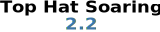
\includegraphics[angle=0,width=0.66\textwidth,keepaspectratio='true']{graphics/title.pdf}
    \end{center}
    \begin{center}
      \normalfont\huge\textsf{\textbf{der} Quelloffene-Segelflugrechner für fast jede Hardware}\par
    \end{center}
    \vskip 1cm
    \begin{center}
      \normalfont\huge\textsf{\@title}\par
    \end{center}
    \vskip 1cm
  \end{maxipage}

  \vfill
%  \todo[nolist,size=\large,inline]{es gibt immer was zu tun}

  \begin{flushright}
    \large \strut {
      \sf
      \today \\
      Für \xc Version \version \\
      \xcsoarwebsite{} \\
    }
    \par
  \end{flushright}
  \par
  \vfil
  \vfil
  \null
  \cleardoublepage
}

\DeclareUnicodeCharacter{00B0}{$^{\circ}$}

\begin{document}

%%%%%%%%%%%%%%%%%%%%%%
% Front page
\maketitle

 
%%%%%%%%%%%%%%%%%%%%%%
% Table of contents
\begingroup
\fontfamily{ptm}
\normalsize
\fontseries{c}\selectfont
\setlength{\parskip}{0.05\baselineskip}
\tableofcontents
\endgroup


%%%%%%%%%%%%%%%%%%%%%%
\chapter*{Preface}

\section*{Cuidado e Precauções}

\warning É DE RESPONSABILIDADE DO USUÁRIO QUE FAÇA A
UTILI\-ZAÇÃO DESTE SOFTWARE COM PRUDÊNCIA. ESTE
SOFTWARE TEM O OBJETIVO DE SER UTILIZADO SOMENTE
COMO AUXÍLIO À NAVEGAÇÃO E NÃO DEVE SER UTILIZADO
PARA NENHUM PROPÓSITO QUE NECESSITE MEDIÇÕES
PRECISAS DE DIREÇÃO, DISTÂNCIA, LOCALIZAÇÃO OU
TOPOGRAFIA. ESTE SOFTWARE NÃO DEVE SER UTILIZADO
COMO AUXÍLIO PARA DETERMINAR A PROXIMIDADE COM O
SOLO PARA NAVE\-GAÇÃO AÉREA. ESTE SOFTWARE NÃO DEVE
SER UTILIZADO COMO UM SISTEMA ANTI-COLISÃO AÉREA.



%%%%%%%%%%%%%%%%%%%%%%
\section*{Notas Legais}

\subsection*{Acordo de licença de Software}

Este software é lançado de acordo com a GNU - General Public License
Versão~2. Veja Anexo~\ref{cha:gnu-general-public} para o texto completo do acordo e notas de
garantia.

\subsection*{Responsabilidade Limitada}

Em nenhuma circunstância o XCSoar, ou seus responsáveis, acionistas,
diretores, empregados, afiliados, contratados, subsidiários ou
organizações proprietárias, serão imputados por qualquer incidente,
danos punitivos ou qualquer outro dano relativo ao uso deste produto.

\subsection*{Reivindicações}
Este produto e todos os arquivos que o acompanham, dados e materiais,
são distribuídos “no estado” em que se encontram, sem qualquer
garantia alguma, exceto o que está impresso ou escrito. Este produto
deve ser utilizado sob risco total do usuário. Todavia, foi tomado os
devidos cuidados durante seu desenvolvimento para eliminar defeitos
para ser um produto sem falhas. Nenhuma reivindicação pode ser legal
a respeito da confiabilidade ou aptidão do produto por nenhum
propósito particular. Os projetistas do XCSoar e seus contribuidores não
devem ser responsabilizados por erros internos ou danos, perda de dados
ou injúria pessoal com a conexão com o dispositivo, desempenho ou uso
deste material.


%%%%%%%%%%%%%%%%%%%%%%
\chapter{Einführung}\label{cha:introduction}\index{Einführung@\hypertarget{Einführung}{Einführung}}
Dies ist das \textsf{XCSoar} - Handbuch, geschrieben für \textsf{XCSoar} - Anwender. 

 

\textsf{XCSoar} ist ein Segelflugrechner-Programm, welches ursprünglich einmal für den Segelflugrechner \al der Firma Triadis geschrieben wurde.  
Anschließend waren die vor ca. 10 Jahren aufgekommenen PocketPC das Ziel, in der Zwischenzeit läuft \textsf{XCSoar} jedoch auf fast allen Plattformen und ist derzeit auf Android mit der derzeit 
sehr performanten Hardware zum Laufen gebracht worden. 

Diese Hardware eignet sich ideal, da die allermeisten der Geräte zwischenzeitlich über GPS- und Lagesensoren und einen 
meist recht fixen Prozessor mit entsprechend RAM verfügen, von denen die PDA damals nur zu träumen wagten - und dennoch 
läuft das Program auch dort hervorragend. 


Es wird hier vorausgesetzt, daß der Leser über Grundbegriffe des Fliegens insbesondere des Überlandfluges 
und über die MC-Theorie verfügt, denn ein Lehrbuch für das Fliegen an sich ist das hier nicht.


Es werden regelmäßig Updates herausgebracht, dem Benutzer ist empfohlen, hin und wieder auf der offiziellen Homepage nach zuschauen. 

Man sollte sich die ''release notes'', also die Veröffentlichungen zu den jeweiligen Versionen ansehen, um  auf evtl.\ Änderungen innerhalb des Programmes gefasst zu sein. 
Die komplette Dokumentation ist erhältlich auf  
\begin{center}
\url{http://www.xcsoar.org}
\end{center}
Da \textsf{XCSoar} ein internationales, offenes Projekt ist (an dem jeder mitmachen kann), sind sogut wie alle Vorgänge und Hinweise auf der Homepage auf Englisch. 
Es ist jedoch inzwischen auch ein deutsches Forum gegründet worden, auf dem man sich Informationen holen kann und mit anderen Anwendern über das ein oder anderen auch über Hardware diskutieren kann.
\begin{center}
\url{http://forum.xcsoar.org/viewforum.php?f=14}
\end{center}
oder aber unten auf $<$deutsch$>$ klicken

\section{Einteilung diese Handbuches}
Das Handbuch ist geschrieben, um den Piloten die bestmögliche Unterstützung bzw.\ Einleitung in das Programm zu geben. 
Wir haben uns bemüht, dies vor allem aus Pilotensicht darzustellen (und hoffen, daß das gelungen ist) 

Dies Kapitel beschäftigt sich vor allem mit dem Herunterladen und Installieren des Programmes. 
In Kapitel~\ref{cha:interface} wird auf das Bedienungskonzept eingegangen und soll einen Überblick über das Aussehen des Programmes geben.

Das Kapitel~\ref{cha:navigation} beschreibt die Kartendarstellung ''Moving Map'' im einzelnen  und zeigt, wie das Programm allgemein 
zur groben Unterstützung der benutzt werden kann. Kapitel~\ref{cha:tasks} zeigt auf, wie Überlandflüge geplant, eingegeben, geflogen und gespeichert werden, und bietet eine Übersicht
der Werkzeuge zur Analyse des aktuellen Fluges, um dem Piloten zu helfen,  seine Performance zu steigern.
Im Kapitel~\ref{cha:glide} geht es weiter ins Detail des Segelflugrechners. 
Es ist wichtig, sich mit diesen Details vertraut zu machen, da hier bestimmte Routinen des Programmes erläutert werden.
Externe Sensoren angeschlossener Geräte, Wetter und Atmosphäre werden in Kapitel\ref{cha:atmosph} behandelt, um zu zeigen, wie das Programm 
sich Konvektionsvorhersage, Wind und Thermik in eine \textsf{XCSoar}-interne Wettervorhersage und Flugplanung einbinden läßt.  
Im Kapitel~\ref{cha:airspace} wird beschrieben, wie \textsf{XCSoar} mit Lufträumen umgeht, davor warnt und diese darstellt. 
Weiterhin werden Kollisionswarnungen, welche durch das \fl-System ermittelt werden können behandelt.
Unter dem Abschnitt~\ref{cha:avionics-airframe} wird aufgezeigt, wie sich \textsf{XCSoar} mit diversen anderen Geräten und Systemen 
verbinden läßt z.B.\ auch der Steuerung über externe Schalter wie z.B.\ Wölbklappenschaltern. 

Der Rest des Handbuches beschäftigt sich hauptsächlich mit Referenzmaterial:

Kap.~\ref{cha:infobox} beschreibt die Funktion und den Inhalt der vorhandenen Infoboxen, die auf dem Bildschirm von \textsf{XCSoar} ausgewählt und angezeigt werden können.
Die Konfiguration des Programmes wird in Kap.~\ref{cha:configuration} ausführlich beschrieben. 
Die Formate der einzelnen Files und Daten, welche von \textsf{XCSoar} benutzt, im- und exportiert werden und wo diese zu finden sind, 
wird in Kap.~\ref{cha:data-files} aufgeführt. 

Zum Schluß soll eine kurzer Überblick über die Historie und den Entwicklungsgang von \textsf{XCSoar} zeigen, wie das Programm zu dem wurde, was 
es derzeit ist\dots Bei Interesse: Kap.~\ref{cha:history-development}.

\section{Notes}


\subsection*{Terminologie}
Im Handbuch werden einige Abkürzungen benutzt, welche evtl.\ --aber hoffentlich nicht--  erklärungsbedürftig sind.

So  steht z.B.\  PDA oder ''Organizer'' für eine Reihe von Geräten, welche es mittlerweile schon kaum noch 
gibt, da die Android-Geräte den Markt unglaublich schnell überschwemmen\dots  
{\small Lediglich eine Clique von Segelfliegern deckt sich mit den alten Ipaq ein, da diese für derzeit 15-25Euro in der Bucht 
zu ersteigern und absolut geeignet sind, um mit \textsf{XCSoar} zu funktionieren}

PDA steht für ''Portable Digital Assistant'' (mobiler digitaler Assistent auf rau-Deutsch). 
Ein PNA ist ein ''personal navigation assistant'' also ein ''privater Navigations Assistent ein NAVI!!

Naja\dots Auch die ''organizer'' gehören dazu - also ''Aufräumer'' oder ''Organisierer'' 
 
Egal, und wie auch immer, innerhalb diese Handbuches sollen diese Bezeichnungen lediglich dafür stehen, 
auf welchen Plattformen und Betriebssystemen \textsf{XCSoar} läuft und eine Gruppe von Anzeigeinstrumenten bezeichnen. 

\textsf{XCSoar} gibt es auch für den Triadis \al - Segelflugrechner. 
Für diesen Rechner wurde \textsf{XCSoar} ursprünglich einmal programmiert. Alles, was in diesem Dokument beschrieben wird, wird also auch 
mit dem \al funktionieren (die andere Bedienweise ausgenommen, da der \al kein Touchscreen ist - ebenso wie PC.)

\subsection*{Bildschirmphotos (Screenshots)}

Im Handbuch werden einige Screenshots dargestellt, um die Bedienung/Funktionalität eindrucksvoller und einfacher darstellen zu können.
Natürlich werden sich diese Screenshots von Gerät zu Gerät unterscheiden, wir gehen aber davon aus, daß es nicht sooo 
schwierig sein wird, eine quer-Darstellung  von der Hochkant-Darstellung zu unterscheiden und hoffen, daß im Zweifelsfalle der geschriebene
Text zur Klärung  beitragen wird. 

Es wird daher mitunter Verwirrung geben, da viele der hier aufgenommenen Bilder in der Hochkant-Ansicht aufgenommen wurden 
--wir können nicht für jedes einzelne Gerät entsprechende Screenshots aufnehmen, das würde dies Handbuch auf 400 Seiten aufblähen! 

Wie gesagt, wir versuchen, diese Photos up2date zu halten, es kann aber auch sein, daß mal ein altes bilde auftaucht.

Im Zweifel gilt der geschriebene Text!!!

\section{Plattformen}
\begin{description}
\item[Windows PC]
\textsf{XCSoar} läuft problemlos auf Windows.

Wenn ein GPS angeschlossen und für die Ausgabe der GPS-Daten konfiguriert wurde, kann vollkommen problemlos mit \textsf{XCSoar} gearbeitet 
werden.  (z.B.\ unterwegs auf einem Notebook o.ä.)

Der Simulator läuft ebenfalls vollkommen problemlos, falls keine GPS-Quelle angeschlossen ist!

Jeder, der mit Windows arbeitet und Segelflieger ist (und \textsf{XCSoar} benutzt oder es beabsichtigt), sollte unbedingt die 
PC-Version installieren und am Simulator trainieren!!! 
\item[Windows Mobile PDA/PNA]
PDA und PNA mit Windows mit Microsoft Pocket PC 2000 bis hinzu Windows Mobile 6 laufen mit \textsf{XCSoar} - der Autor hat einen Ipaq3850 seit Jahren 
auch auf Wettbewerben im Einsatz. Es geht!!

Windows Mobile 7 ist nicht unterstützt, da Microsoft entschieden hat, keine Unterstützung für Entwickler dieses 
Betriebssystemes zu geben.
\item[Unix/Linux PC]
\textsf{XCSoar} kann problemlos am WINE-Emulator laufen, es läuft aber auch (seit V6.0x) nativ für die Debian/UBUNTU) Versionen.
\item[Android Devices] \textsf{XCSoar} läuft auf Android 1.6 oder neuer 
\item[\al] Der \al ist ein Segelflugrechner welcher fabrikmäßig mit \textsf{XCSoar} als Software ausgestattet ist. 
Die \al-PRO-Version enthält ein integriertes GPS.
\end{description}


\section{Technische Unterstützung / Support}

\subsection*{Troubleshooting}
Ein kleines Team von freiwilligen, nicht bezahlten Leuten entwickelt und programmiert \textsf{XCSoar}. 

Obwohl wir gerne helfen, können wir nicht jede Frage beantworten, welche sich z.B. mit einem 
Hardware Fehler ''Mein  Galaxy SII bootet nicht mehr'' beschäftigt. Wir denken, das ist unmittelbar einleuchtend.

Es gilt, Software von Hardware zu trennen. 

Wenn Du Fragen zu \textsf{XCSoar} hast, sende eine --konkrete-- mail an: 

\begin{quote}
\url{xcsoar-user@lists.sourceforge.net}
\end{quote}
oder stelle deine Frage auf dem User Forum:
\begin{quote}
\url{http://forum.xcsoar.org/}
\end{quote}

Alle häufig auftretenden Fragen werden gesammelt und zur Website weitergeleitet, wo sie behandelt werden.
Du kannst an die die mailing list schreiben, um aktiv informiert zu werden, sowie Neuigkeiten stattfinden: 

Mehr dazu auf der \textsf{XCSoar}-Homepage. 
\begin{quote}
\xcsoarwebsite{}
\end{quote}

Das beim Start von \textsf{XCSoar} erzeugte log-file \verb|xcsoar-startup.log| ist hilfreich für die Analyse von Fehlern und kann  
mit einem kleinen Bericht zu den Entwicklern gesendet werden, um Fehlern auf die Spur zu kommen 
und \textsf{XCSoar} permanent zu verbessern. 

Für \al Benutzer: dies Files wird vom \al auf das ''FromAltair'' Verzeichnis geschrieben, von wo es aus kopiert 
und eingesendet werden kann. 

\subsection*{Updates}
Du solltest periodisch nachschauen, ob Neuerungen/neue Versionen  bzgl.\ \textsf{XCSoar} auf der HP zu finden sind. 
Die Installation ist immer die gleiche; alle vom Bediener erstellten Files wie Konfiguratiobnsfiles 
bleiben beim Update bestehen und können später wieder benutzt werden. Die Updates auf der Android Plattform können -- je nach Einstellungen auf Deiner Hardware  (automatische updates erlaubt\dots)-- vollkommen automatisch erfolgen! 

Nach wichtigen Files wie Karten, Lufträumen und Wegpunkten zu schauen ist wohl selbstverständlich!


Wie jede komplexe Software kann auch \textsf{XCSoar} Fehler enthalten und ist \textsf{XCSoar} darauf angewiesen, daß diese dem Entwicklerteam zur  Kontrolle/Korrektur zugehen. Keine Rückmeldung--keine Verbesserung!

Hierzu gibt es extra ein Bug-tracking-System, also ein Fehler-Verfolgungssystem, in dem Ihr explizit Fehler melden könnt.

Bitte seht vorher nach, ob nicht ein solcher Fehler bereits gemeldet wurde. 
Doubletten machen unglaublich viel Arbeit und behindern den zügigen Fortgang der Entwicklung --logischerweise.  


Hierzu siehe:  
\begin{quote}
\url{http://www.xcsoar.org/trac/}
\end{quote}
oder einfach eine mail an 
\begin{quote}
\url{xcsoar-devel@lists.sourceforge.net}
\end{quote} 

\subsection*{Updaten von \textsf{XCSoar} auf dem \al}

Ein Update von \textsf{XCSoar} auf dem \al  benötigt als erstes das aktuelle  File {\tt XCSoarAltair-YYY-CRCXX.exe}, 
heruntergeladen z.b.\ auf einen USB-Stick. 

Anschließend wird der Sticke eingeschoben, der \al gestartet und es öffnet sich \al-eigene Bootsoftware, 
innerhalb welcher ein Update angewählt werden kann.

Für Details, schaut bitzte im \al-Handbuch, dem {\em Altair Owner's Manual} nach.
Andere Dateien wie Lufträume, Karten etc. werden auf die gleiche Weise auf den \al kopiert. 

\section{Training}
Es ist grundsätzlich allen Piloten,  insbesondere jedoch denen, die einen Segelflugrechner,  egal welcher Art, an Bord haben, 
dringenst angeraten, aus dem, Fenster zu schauen, anstatt sich ''{\it mit dere olle Gnöbbsche zu befasse\dots}''
\achtung 
Das gilt auch und selbstverständlich für diejenigen, welche \textsf{XCSoar} benutzen. \textsf{XCSoar} fliegt {\sl nicht} allein und hält {\sl nicht} 
die Fahrt und weicht {\sl keinem}  anderen Flugzeug oder Berg aus! 

Aus diesem Grunde ist die Beschäftigung bzw.\ Training mit \textsf{XCSoar} dringend angeraten, {\sl bevor} man es benutzt. 


\subsection*{\textsf{XCSoar} auf dem PC benutzen}
Die PC-Version sollte benutzt werden, um es den meisten (Windows)-Usern es zu erlauben, sich mit \textsf{XCSoar} ein 
bißchen auseinanderzusetzen. 

Da die Konfiguration exakt gleich ist, wie auf den mobilen Geräten, sollte es anschließend keine Schwierigkeit geben,
auch mit dem Handy oder PDA mit \textsf{XCSoar} 'abzuheben''.


Die PC-Version kann ebenfalls an externe GPS-Quellen angeschlossen werden und zu einem 
vollwertigen Navigationssystem ''verwandelt'' werden. 


\begin{itemize}
\item Schließe z.B.\ ein \fl an den PC an und benutze diesen als Bodenstation für \fl-Verkehr
\item Schließe den PC an ein intelligentes Variometer an und teste die die Konfiguration damit  (z.B. Vega)
\end{itemize}

\subsection*{\textsf{XCSoar} zusammen mit einem Flugsimulator benutzen und erlernen}
Es ist eine wirklich außerordentlich gute Idee und bringt echt was, \textsf{XCSoar} zusammen mit einem Flugsimulator zu benutzen, bzw.\ zu erlernen.
Dazu muß der Simulator/der PC die Daten mittels des Standard-NMEA-Protokolles ausgeben können, sodaß  \textsf{XCSoar} diese über den seriellen Port auslesen und interpretieren kann.
{\sc Condor} und {\sc X-Plane} bieten derzeit solche Möglichkeiten.  

Der große Nutzen des Trainings am Boden ist der, daß Du in der Luft die Griffe, Interpretationen der Anzeige und Möglichkeiten, 
die Dir \textsf{XCSoar} bietet ''im Schlafe'' beherrscht. Fliegst Du Wettbewerb, so ist das zumindest im Einsitzer absolut unumgänglich.
Auch ein LX8000 ist nicht innerhalb einer halben Stunde (auch nicht innerhalb einer ganzen) zu beherrschen -- und ich weiß wovon ich spreche\dots


\section{\textsf{XCSoar} sicher und verantwortungsbewußt benutzen}
Die Anwendung eines interaktiven Systemes wie  \textsf{XCSoar}, welches sogar Luftverkehrserkennung bietet, läßt den Benutzer dazu neigen, die Luftraumbeobachtung evtl.\ zu vernächlässigen. 
Es ist nicht unsere Intention, Piloten von der Beobachtung des Luftraumes um sie herum abzulenken,  sondern Ihnen  ein Hilfsmittel an die Hand zu geben,
mit dem u.a.\ die Navigation  und die Berechnung  des Endanfluges vereinfacht wird.

Die Philosophie, die hinter der Entwicklung dieser Software steht, ist die, die Ablenkung des Piloten von der Beobachtung wirklich wichtiger Dinge
wie z.B.\ (und vor allem) des in unmittelbarer Nähe befindlichen Luftraumes so gering wie möglich zu halten.

Hierzu ist vor allem Wert darauf gelegt worden, die Bedienereingaben auf ein Minimum --und wenn, dann so einfach und 
schnell wie möglich-- zu beschränken. 
 
Piloten, die  \textsf{XCSoar} benutzen, sollten sich der Verantwortung durch die evtl.\ Ablenkung durch ein solches Programm/System stets bewußt sein!

Es sollte selbstverständlich sein, folgende Dinge zu beachten:
\begin{itemize}
\item Werdet vertraut mit \textsf{XCSoar}, z.B.\ und insbesondere durch die Bedienung des Programmes z.B.\ mit Hilfe des Simulators
\item Benutze und ''fummele'' an Deinem Gerät erst dann herum, wenn Du {\sl sicher bist, daß der Luftraum {\bf frei} ist}!! 
Mache keine Kurven oder Turns, während Du mit der Bedienung der Software beschäftigt bist!An \textsf{XCSoar} herumspielen kannst Du am Boden. 
Du solltest mit der Bedienung wirklich fit sein, gerade auch im Wettbewerb, oder als ''Beginner''.
\item Konfiguriere Dein System so (es ist möglich und Du kannst es\dots), daß Du die interaktiven Eingaben auf ein Minimum beschränkst und 
jederzeit im Griff hast. (Es werden von \textsf{XCSoar} viele automatische Funktionen angeboten - nutze diese oder --falls nicht vorhanden-- 
frage z.B. das Entwicklerteam,  solche Funktionen zu entwickeln/ implementieren).   
\end{itemize}


%%%%%%%%%%%%%%%%%%%%%%
\chapter{Installation}\label{cha:installation}

To run XCSoar, you need to obtain the following:

\begin{itemize}
\item a device to run XCSoar on
\item XCSoar
\item a GPS receiver
\item a waypoint file
\item an airspace file (optional)
\item a map file (optional)
\end{itemize}

\section{Compatibility}

\subsection*{Devices for running XCSoar}

XCSoar runs on the following platforms:

\begin{itemize}
\item mobile phones and tablets with Android 1.6 or newer \\
  Example: Dell Streak, Samsung Galaxy S II, HTC Desire HD,
  Motorola Xoom
\item Kobo Mini
\item PDAs with Pocket PC 2000, 2002, 2003 \\
  Example: iPaq 3800, iPaq 3900
\item PDAs with Windows Mobile \\
  Example: iPaq hx4700, Dell Axim x51v
\item PNAs with Windows CE 3.0 or newer \\
  Example: HP314, Mio400
\item Triadis Altair
\item LX MiniMap
\item Windows 2000 or newer
\item Linux
\item Mac OS X
\end{itemize}

\subsection*{GPS, Logger, Vario}

XCSoar is compatible with any GPS emitting NMEA data.  Most modern
Android devices have a built-in GPS, but sometimes it is favorable to
connect to an external device:

\begin{itemize}
\item an airspeed indicator allows quick and exact wind estimates
  without circling
\item a vario improves the thermal assistant
\item a task can be declared to an IGC logger, and after landing, the
  flight log can be downloaded
\item some varios allow synchronising the MacCready setting with
  XCSoar
\end{itemize}

\subsection*{Supported external devices and features}
\label{sec:supported-varios}

\newcommand{\y}[0]{{ $\surd$ }}
%{0.8\textwidth}
\noindent\makebox[\textwidth]{%
\begin{tabular}{l|ccc|cc|cc|c}
       \multicolumn{1}{r}{Supported:} & \multicolumn{3}{c|}{-Features} & \multicolumn{5}{c}{-Stream Data} \\
NMEA Device & 
  \begin{sideways} Declaration\end{sideways} & 
  \begin{sideways} Remote ctrl.\end{sideways} & 
  \begin{sideways} Download\end{sideways} &
  \begin{sideways} Airspeed\end{sideways} & 
  \begin{sideways} Vario\end{sideways} & 
  \begin{sideways} Baro. altitude\end{sideways} & 
  \begin{sideways} Wind\end{sideways} &
  \begin{sideways} G-Sensor\end{sideways} \\
\hline
%                    _Decl_Remo_Down_Airs_Vari_Baro_Wind_Gsen_
Borgelt B50          &    & \y &    & \y & \y & \y &    &    \\
CAI 302              & \y & \y & \y & \y & \y & \y & \y & \y \\
CAI GPS Nav          &    &    &    &    &    &    &    &    \\
Condor               &    &    &    & \y & \y & \y & \y &    \\
\hline
Digifly Leonardo     &    &    &    & \y & \y & \y & \y &    \\
EW Logger            & \y &    &    &    &    & \y &    &    \\
EW microRecorder     & \y &    &    &    &    & \y &    &    \\
FLARM                & \y &   & \y  &    &    & \y &    &    \\
\hline
%                    _Decl_Remo_Down_Airs_Vari_Baro_Wind_Gsen_
Flymaster F1         &    &    &    &    & \y & \y &    &    \\
Flytec 5030          &    &    &    & \y & \y &    &    &    \\
GTAltimeter          &    &    &    &    &(\y)& \y &    &    \\
ILEC SN10            &    &    &    &    & \y & \y & \y &    \\
\hline
IMI ERIXX            & \y &    & \y &    &    &    &    &    \\
LX20, Colibri        & \y &    & \y &    &    & \y &    &    \\
LX Vario \footnotemark
                     & \y & \y & \y & \y & \y & \y & \y & \y \\

LXNAV Nano           & \y &    & \y &    &    &    &    &    \\
\hline
%                    _Decl_Remo_Down_Airs_Vari_Baro_Wind_Gsen_
LXNAV V7             &    & \y &    & \y & \y &    &    &    \\
PosiGraph            & \y &    &    &    &    & \y &    &    \\
Triadis Altair (pro) & \y &    &    &    &    & \y &    &    \\
Triadis Vega         &    & \y &    & \y & \y & \y &    & \y \\
\hline
Volkslogger          & \y &    & \y &    &    & \y &    &    \\
Westerboer VW1150    &    & \y &    & \y & \y & \y &    &    \\
Westerboer VW921, 922
                     &    & \y &    & \y & \y & \y &    &    \\
Zander / SDI         &    & \y &    & \y & \y & \y & \y &    \\

\end{tabular}}
\footnotetext{LX Navigation offers a variety of intelligent vario 
  devices such as LX1600, LX5000, LX7000. They all share their NMEA functionality. 
  The offered functionality in connection to XCSoar depends on 
  last not least e.g. the vario's firmware revision. }

While most Windows CE based devices have a serial port, such legacy
hardware is not present in modern Android devices.  Those can either
use Bluetooth or the Android IOIO board.  To use Bluetooth, you need
to connect the external device to a Bluetooth-to-Serial adapter, such
as the K6-Bt or the Glidertools VFBT-1.


\section{Software installation}

The software is available as a free download from the XCSoar website
~\xcsoarwebsite{}.  This section describes which file should be
downloaded, and how to install it.

\subsection*{On Android}

Obtain XCSoar from Google's Android market, or install the \verb|apk|
file manually.  Copy the data files on the SD card in the directory
\verb|XCSoarData|.

\subsection*{On a Kobo Mini}

The Kobo Mini is a cheap e-book reader.  It has a black and white
e-paper screen with excellent sunlight readability.

Before you begin: back up the internal SD card.  The XCSoar installer
may break the Kobo, though unlikely.  You can always recover the Kobo
from a software failure, but only if you have access to a backup.

To install XCSoar, connect the Kobo to your PC via USB.  The Kobo
exposes a mass storage device to your PC; open it and create a
directory called \texttt{.kobo} (note the leading dot).  Download the
file \texttt{KoboRoot.tgz} from the XCSoar website into that
directory (\url{http://www.xcsoar.org/hardware/}). Unplug the Kobo and reboot it (switch it off completely,
and switch it on again).  You will see the message ``Updating'', and
after a few minutes, the Kobo shows a menu that allows you to launch
XCSoar or the Kobo e-book reader software.

To copy data files (maps, waypoints, ...) to the Kobo, launch the
original Kobo software (``Nickel'') and connect the Kobo to your PC
again.  Copy the files into a directory called \texttt{XCSoarData} at
the top level.

\subsubsection{Hacking the Kobo}

After installing XCSoar on the Kobo, the new boot script checks for a
script called \texttt{XCSoarData/kobo/init.sh} and executes it.  If
you know what you're doing, you can use this script to do things at
boot time, for example launch \texttt{inetd} (for \texttt{telnet}
access).

\subsection*{On a PDA (Windows Mobile, PocketPC)}

Choose one of the targets:

\begin{description}
\item[\texttt{PPC2000}] Pocket PC 2000/2002, Windows CE 3.0
\item[\texttt{PPC2003}] Pocket PC 2003, Windows CE 4.0
\item[\texttt{WM5}] Windows Mobile 5 or newer
\item[\texttt{WM5X}] Windows Mobile 5 or newer with XScale CPU or
  better (e.g. hx4700)
\end{description}

Download the program file \verb|XCSoar.exe| to a SD card.  You can
launch it with the File Explorer.
\sketch{figures/XCS_Today.png}
Another method to install XCSoar on a PDA is the CAB file.  Download
it to the SD card.  Use the File Explorer to install it.  After the
installation, the XCSoar `FLY' and `SIM' launcher icons will be
visible on the Today screen.


\subsection*{On a PNA (Windows CE)}

Download the program file \verb|XCSoar.exe| (target ``WM5'') to a SD
card.  You can launch it with the File Explorer.

\subsection*{On a Windows PC}

Download the program file \verb|XCSoar.exe| (target ``PC'') to your
hard disk.

\subsection*{On Unix/Linux}

The file downloaded is \verb|xcsoar_XXX.deb|, where \verb|XXX| includes
the version number and platform, e.g. \verb|xcsoar_6.0.4_i386.deb|.
The is a Debian package and can be installed using 
\begin{center}
\verb|sudo dpkg -i xcsoar_XXX.deb|.
\end{center}
Use \verb|dpkg-query -L xcsoar| to see where the executable and 
other files are installed,
Additional data files must be placed in the directory
\verb|~/.xcsoar|.
If \verb|~/.xcsoar| does not exist, it will be created the first time
that \verb|xcsoar| is run.


\section{Data files}

To be able to use XCSoar's advanced features, additional data files, such as
terrain, topography, special use airspace, waypoints etc.\ are needed. The files
that can be used with XCSoar are described in Chapter~\ref{cha:data-files}.

All data files should be copied into the directory
\texttt{XCSoarData}.  This directory must be in a specific place
so that XCSoar knows where to look for data files:

\begin{description}
\item[Windows PC]
\texttt{XCSoarData} is in your personal folder (``\texttt{My
Documents}'')
\item[Windows Mobile PDA/PNA]
If there is a directory named \texttt{XCSoarData} in the same
directory as \texttt{XCSoar.exe}, then this one will be used.
\texttt{XCSoarData} is on the SD card.  If there is no SD card, then
XCSoar looks for it in \texttt{My Documents}.
\item[Unix/Linux]
The directory is called \verb|.xcsoar| in the user's home directory.
\item[Android Devices]
\texttt{XCSoarData} is on the SD card.
\item[Altair]
If XCSoarData exists on an USB drive, that one is used, otherwise the
internal storage is used.
\end{description}


XCSoar will generate a number of additional files at run time.  These
will be placed in the  \texttt{XCSoarData} directory (Windows PC and 
Windows Mobile devices), or the \texttt{.xcsoar} directory (Unix/Linux
PC).  At first run, XCSoar will create the files 
\texttt{Default.tsk} (Default Task),  \texttt{default.prf} 
(configuration settings), \newline
\texttt{xcsoar.log} (log of the startup progress), 
plus three directories: \texttt{cache},
\texttt{config} and \texttt{logs}.  Additional files may be
created/modified while XCSoar is running, such as task files
(\texttt{*.tsk}) and flight logs.


\section{Running XCSoar}
%\subsection*{Fly and simulator modes}

Two modes are available inside the XCSoar application: 
\begin{description}
\item[FLY] This mode is used when actually flying.  The simulator is 
  disabled and serial communications are active. 
\item[SIM] This starts XCSoar in simulator mode, no serial communications
  are attempted.
\end{description}

\subsection*{Altair version}
XCSoar starts up automatically when Altair is powered on.
The PWR/ESC button (top left) has multiple functions:
\begin{description}
\item[Powering on]  Press and hold the PWR/ESC button for one second.
  The LED in the button will light up, and XCSoar will start after
  Altair has booted.
\item[Powering off]  Press and hold the PWR/ESC button for 3 seconds.
  Altair will switch off.
\item[Escape] Pressing the PWR/ESC button quickly acts as an
Escape key, typically used to close dialog pages or as a cancel function.
\end{description}

The Altair version of XCSoar does not include a simulator mode.

\subsection*{XCSoar PC version}
The program can be run by opening the explorer window, finding the directory
that has the XCSoar.exe executable, and double clicking on that program file.

The program command line options allows the screen orientation of
the display to be defined:
\begin{description}
\item[-portrait] The screen is 480 pixels wide, 640 pixels high.
\item[-square] The screen is 480 pixels wide, 480 pixels high.
\item[-landscape] The screen is 640 pixels wide, 480 pixels high. This is the
usual setting. If you don't specify this parameter the landscape version will be
loaded automatically.
\item[-small] Draws the screen at half size.  This is useful for using XCSoar in
 conjunction with flight simulators e.g.\ Condor.
\end{description}
To change the screen orientation, it is convenient to create a shortcut to the
program, then right click on the shortcut icon and click on ``Shortcut''. 
In the field ``Target'' add one of the desired options listed above.

\subsection*{XCSoar Unix/Linux PC version}
Run \verb|xcsoar| from a command line, or create a shortcut on the
desktop.  The location of the executable file may be found using
\verb|which xcsoar|.  Only landscape mode is  supported for now.

\subsection*{Loading data files}
The first time that XCSoar is run, it does not automatically load the 
data files that you placed in the \verb|XCSoarData| directory.  
To tell XCSoar which files to load, double click/tap the map (the large,
blank white part with the glider symbol in the center),
choose the menu \bmenu{Config 2} (click/tap it twice), then select the item 
\bmenu{System}.  The Configuration screen should be displayed:
\sketch{figures/config-basic.png}
The first page allows you to choose the map, 
waypoint and airspace files, by clicking/tapping on the text boxes.
Many other features of XCSoar may be configured here. These are described in detail in Chapter
\ref{cha:configuration}.
Once completed, XCSoar reloads those files; from now on, the data files
will be loaded automatically at run time.

\subsection*{Start-up and user profiles}
When XCSoar starts up, it will check for existing profiles. If multiple
profiles are detected it will displays a small window asking you which profile
to load. To proceed, choose the desired profile and press Enter. If no
profile is chosen the settings from the last session are loaded again. Profiles
can be useful for example in the following cases:
\begin{itemize}
\item Different pilots
\item Competition versus casual flying
\item Flying in different locations
\end{itemize}


\subsection*{SIM mode}
The simulator contains a simple interface allowing the user to fly
the glider about.  On the map screen, clicking/touching the glider symbol
(with touchscreen or mouse) and dragging 
causes the glider to move in the direction of the drag, the
speed being proportional to the length of the drag.  

In the PC version and for embedded devices with buttons, the aircraft
speed, altitude and direction may be changed using the \InfoBox es.
These features are not available for touchscreen devices.
The aircraft altitude can be adjusted by selecting the GPS altitude
{\InfoBox} (marked \infobox{Alt GPS}), and pressing the up or down key.
The airspeed  can be adjusted by selecting the ground speed
{\InfoBox} (marked \infobox{V Gnd}), and pressing the up or down key.
The glider's track  can be adjusted by selecting the track
{\InfoBox} (marked \infobox{Track}), and pressing the up or down key.
With either of the \InfoBox es \infobox{Alt GPS} or \infobox{V Gnd})
selected, the glider's direction may be changed using the left/right keys.

Other controls, buttons and menus work the same as in FLY mode.


\subsection*{Splash screen}
When XCSoar starts up, shuts down, or loads large files, such as airspace,
waypoints, terrain, etc., a progress screen is presented while the data is being
loaded. This screen has a progress bar which indicates the data loading
activity, and a short line of text describing the action that is being performed.

This screen also displays the software version information.

\subsection*{Exiting the program}
For PDA and PC versions, XCSoar is shut down from the menu. The menu can be
opened by double-clicking on the map or the \InfoBox es.
\begin{quote}
\bmenu{QUIT}
\end{quote}

For PC versions, XCSoar can also be shut down by clicking the close icon
on the XCSoar window.

For Altair, XCSoar is shut down by holding the PWR button for two seconds or
more.


%%%%%%%%%%%%%%%%%%%%%%
\chapter{Benutzeroberfläche}\label{cha:interface}

Dies Kapitel beschreibt das grundlegende  Konzept der Benutzeroberfläche, wie sie von \textsf{XCSoar} benutzt wird und ist als erste Übersicht zu verstehen. Mehr Details werden in den folgenden Kapiteln erörtert.

\begin{center}
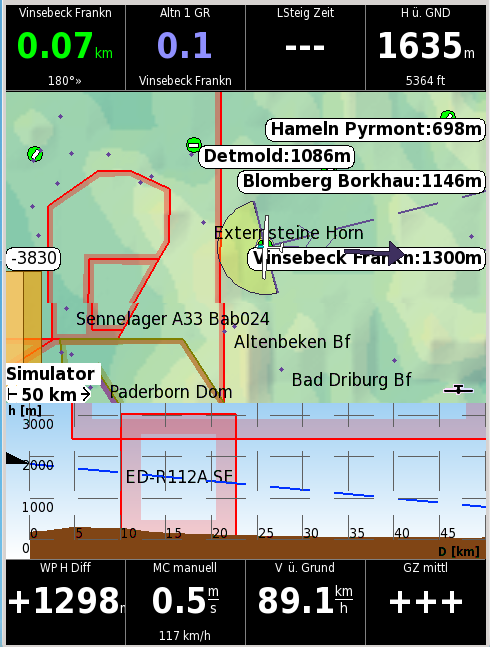
\includegraphics[angle=0,width=0.75\linewidth,keepaspectratio='true']{figures/plain.png}
\end{center}

Die  \textsf{XCSoar} Anzeige besteht aus mehreren Teilen:
\begin{description}
\item[\p{Kartenanzeige}] Die größte Fläche des Bildschirmes wird vom GPS-moving map beansprucht.
Wichtige Symbole, welche Informationen des Segelflugrechners darstellen, werden auf dieser Karte
eingeblendet (z.B. die Über/Unter Gleitpfad-Pfeile am linken Rand oder das Thermik-Höhenband).
Einige Icons und Textinformationen  erscheinen  (bei Bedarf) am unteren Rande des Displays,
welche über den Zustand des Rechners (verbunden mit GPS, Kurbelmodus, Endanflugmodus) etc.\  informieren.
%
\item[\p{{\InfoBox}en}] Eine bislang nur rechteckige Anordnung von sogenannten Info-Boxen, welche mit diversen Angaben, wie zum Beispiel Geschwindigkeit über Grund,
Höhe, MC Cready, geschätzte Zeit zum nächsten Wegpunkt usw. gefüllt ist, kann entweder am oberen und unteren Rand, rechts oder links,
oder auf der rechten Seite des Displays (im Quer- bzw. landscape-Modus) angezeigt werden. Bislang sind diese Anordnungen fix, in zukünftigen Versionen ist jedoch angestrebt, diese Infoboxen auch frei verschiebbar auf dem Display anordnen zu können.
%
hier werden diejenigen Werte, die der Benutzer vorher ausgewählt  hat und von \textsf{XCSoar} bzw. angeschlossenen Geräten ausgewertet werden, angezeigt.
%
\item[\p{Anzeigen}] Anzeigen stellen Instrumenten Displays dar (z.B. ein Vario). Alle Anzeigen sind optional und einige
haben lediglich informellen  Character, wenn \textsf{XCSoar} an ein unterstütztes Instrument angeschlossen ist.
%
\item[\p{Button Beschriftungen and Menüs}] Hardware-Knöpfe und die Wippe des Gerätes, auf dem \textsf{XCSoar} läuft, können benutzt werden, um Menüs bzw.\ Hauptmenüs aufzurufen, welche typischerweise den Hardwareknöpfen und /oder der Wippe fix zugeordnet sind. Dies erlaubt mitunter einen schnelleren Zugriff als das Bedienen allein des berührungsempfindlichen Bildschirmbereiches ("TouchScreen").
Falls das entsprechende Gerät über einen solchen TouchScreen verfügt (nahezu alle bis auf \al), können alle Menüs auch
hierüber geöffnet und bedient werden. Diese Buttons sind in schwarzem Text auf hellgrünem/grauen Hintergrund gestaltet.
%
\item[\p{Status Meldungen}] Hinweise zum Status des Fluges und auch des Flugzeuges  (z.B.\ Annäherung an einen Luftraum, vergessenes Fahrwerk, Startbestätigung bei Überfliegen der Start/Ziellinie etc\dots ) wird in einer Textbox  über dem Bildschirm eingeblendet.
Dieser Status Meldungen werden angezeigt, um detaillierte, wichtige Informationen zu geben, wenn gewisse, zum Teil konfigurierbarer Ereignisse, auftreten.
%
\item[\p{Dialog Fenster}] Die -größeren- Dialogfenster enthalten normalerweise Grafiken und Buttons. Diese werden verwendet, um dem Piloten  detaillierte Daten bezüglich Wegpunktdetails, Statistik und Analyse des bisherigen Fluges, Polaren etc\dots  zu übermitteln.

\item[\p{Hauptmenü}] das Hauptmenü wird entweder über einen Doppelklick auf die Bildschirmoberfläche oder aber über Gesten \gesture{Runter - Hoch} aufgerufen.

   Wenn die erscheinenden Buttons nicht innerhalb einer gewissen (einstellbaren) Zeit  betätigt  werden, verschwinden sie von sich aus wieder, um die Kartendarstellung des weiteren Fluges nicht zu behindern.
\end{description}

Die Bedienung von \textsf{XCSoar} ist auf verschiedene Wege möglich:

\begin{itemize}
\item Anklicken eines speziellen Kartenelements
\item Anklicken einer InfoBox und anschließend den Bildschirmmenüs
\item Benutzen einer "Geste", z.B. Zeichnen eines Striches von links nach rechts auf dem TouchScreen
 (siehe dazu Kap.~\ref{sec:gestures} weiter unten).
\item "Verschieben" (dragging) des Bildschirms (berühren und verschieben auf dem TouchScreen unter Fingerdruck).
\item Drücken der Hardware-Knöpfe des  Gerätes.
\item Drücken der Wippe des Gerätes.
\item Drücken  oder Schalten  an einem an \textsf{XCSoar} angeschlossenen Gerät.
\end{itemize}

Je nachdem, welcher Hardware bzw.\ welches Gerät mit \textsf{XCSoar}  benutzt wird, stehen nicht alle dieser Methoden zur Verfügung. Die Belegung der jeweiligen Hardware-Knöpfe können daher unterschiedlich sein.

Bei der \textsf{PC}-Version von \textsf{XCSoar} ist das Anklicken eines Bildschirmelements es mit der Maus identisch der Berührung mittels Touchscreen.

Da der \al nicht über einen TouchScreen verfügt, ist hier die Belegung der Menüs und Elemente grundlegend anders und wird über die dort vorhanden Hardware-knöpfe und Drehgeber vorgenommen.

 \newpage
 \section{Grundlegende Layouts von\textsf{XCSoar}}
 \textsf{XCSoar} läßt sich von der Oberfläche her extrem flexibel anpassen, je nach Geschmack des Benutzers. 
 Ich will hier lediglich vier unterschiedliche Darstellungen zeigen, welche allesamt im Konfigurationsmenü eingestellt werden können. 

 \begin{center}
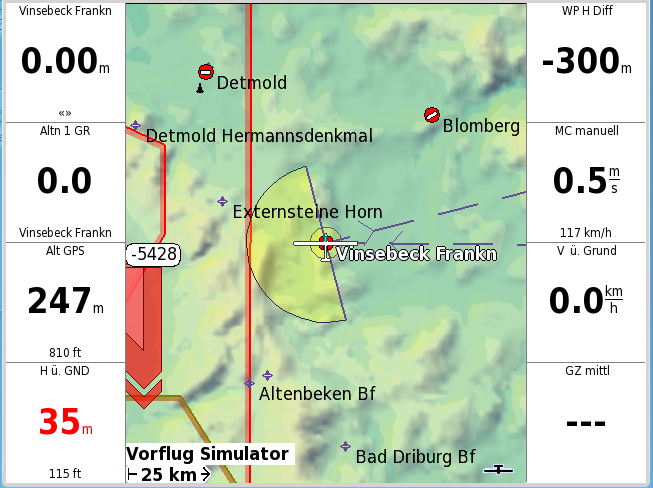
\includegraphics[angle=0,width=0.45\linewidth,keepaspectratio='true']{figures/map-outfit2.png}\quad
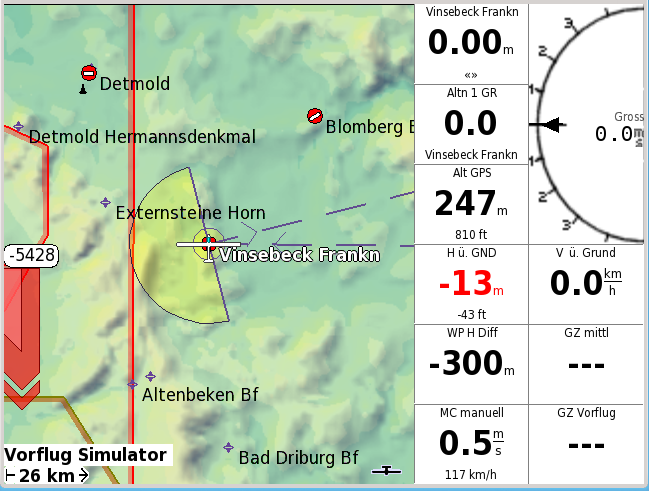
\includegraphics[angle=0,width=0.45\linewidth,keepaspectratio='true']{figures/map-outfit3.png}\vspace{1em}
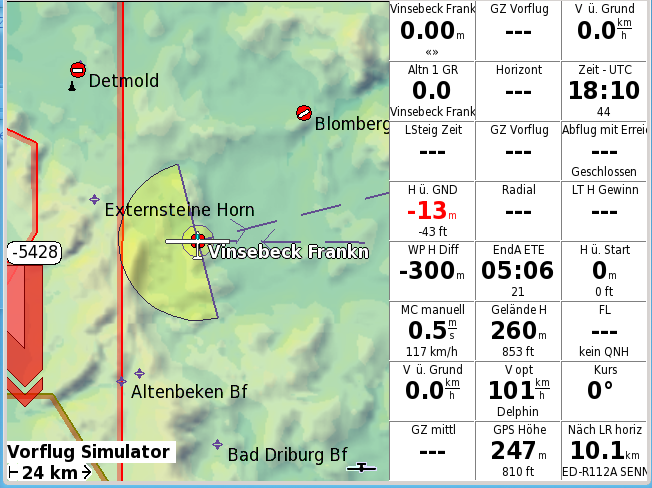
\includegraphics[angle=0,width=0.45\linewidth,keepaspectratio='true']{figures/map-outfit4.png}\quad
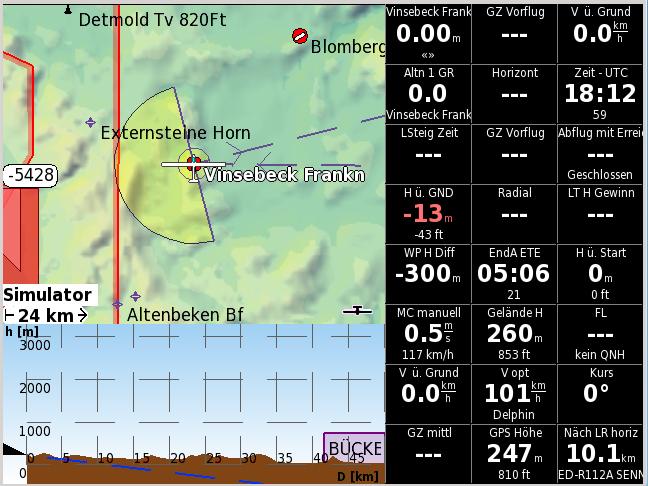
\includegraphics[angle=0,width=0.45\linewidth,keepaspectratio='true']{figures/map-outfit5.png}\vspace{1em}
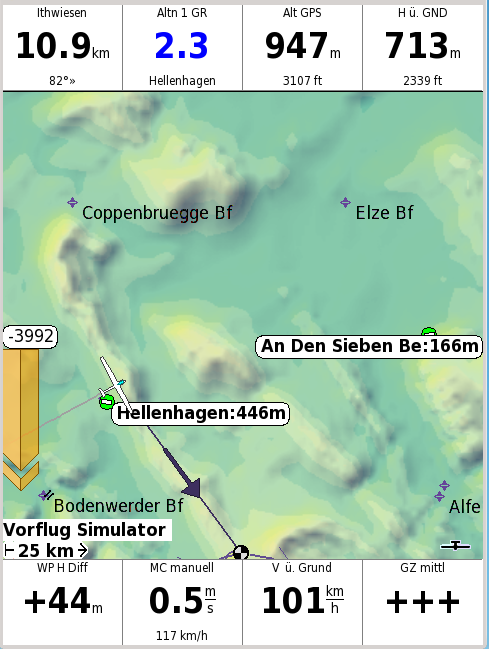
\includegraphics[angle=0,width=0.45\linewidth,keepaspectratio='true']{figures/map-outfit1.png}\quad
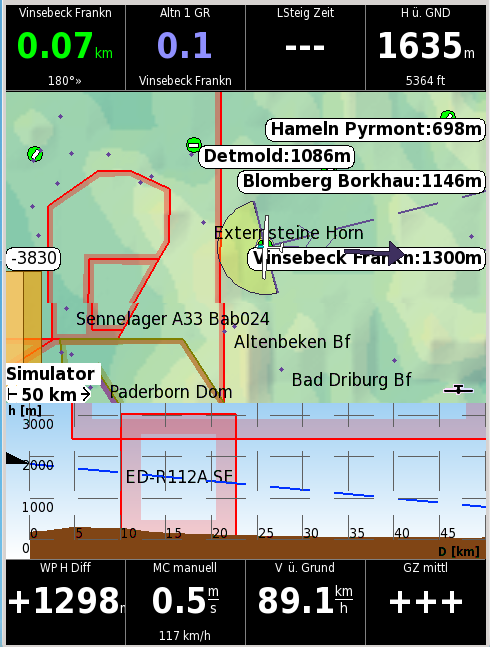
\includegraphics[angle=0,width=0.45\linewidth,keepaspectratio='true']{figures/map-outfit6.png}
\end{center}
Ob hochkant, quer, quadratischt schwarz oder weiß, mit Vario oder ohne, auch komplett ohne Infoboxen - alles möglich.
Die Einstellungsvarianten mögen auf den ersten Blick schier unübersichtlich sein, innerhalb weniger Tage oder Flüge jedoch habt ihr mit Sicherheit Eure Lieblingskonfiguration gefunden.


Ich beschränke mich in diesem Handbuch  grundsätzlich auf die hocjhkant (Portrait) Darstellung, da fats alle älteren PDA nur für diese geeignet erscheinen. Bei moderneren Android Geräten mag dies anders ein. Kann ja jeder machen wie er lustig ist.
   
 \newpage\section{Button-Beschriftungen und -Menüs}
Das Button-Menü besteht aus einem Satz von Buttons und Menüs und ist wird -bis auf die o.g. genannten Ausnahmen- mittels des TouchScreens aufgerufen (Doppelklick auf die berührungsempfindliche Oberfläche).

Die Benutzung der Buttons und des Button-Menüs  stellt die bevorzugte Art der Interaktion mit \textsf{XCSoar} dar.

\begin{center}
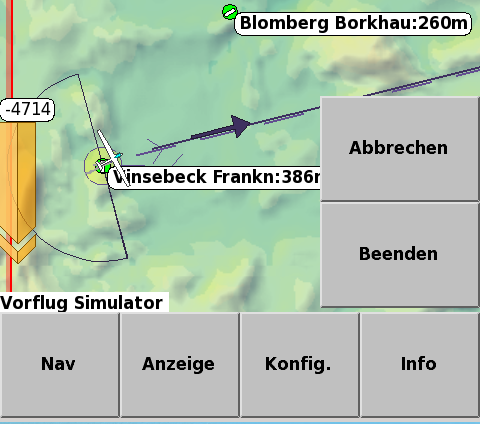
\includegraphics[angle=0,width=0.75\linewidth,keepaspectratio='true']{figures/buttonmenu.png}
\end{center}

\subsection*{Grundlegende Info zur Bedienoberfläche}
Das Menü ist in vier Hauptgruppen mit hoffentlich aussagekräftigen Namen (\textbf{Nav}, \textbf{Anzeige}, \textbf{Konfig.} und \textbf{Info}) unterteilt, welche diverse Untermenüs besitzen. Das spezielle Layout hängt vom jeweils benutzten Gerät ab und kann ebenso vom Bediener angepaßt werden. \textbf{Beenden} und \textbf{Abbrechen} vertseht sich wohl von slebst. 

 \textsf{XCSoar} kann ebenso über an das Gerät angeschlossene externe Eingabegeräte wie Joysticks, externe Tastaturen, game-pads und Multifunktionsgriffe bedient werden. Die hierüber aufzurufenden Funktionen können in großem Rahmen eben falls frei konfiguriert  werden.


Beim  \al  gibt es vier Hauptmenüs, welche durch Drücken auf die Knöpfe an der linken Seite aufgerufen werden können. 

Sowie ein Menü aktiviert wurde, erscheinen Untermenüs mit entsprechenden Beschriftungen über der unteren Druckknopfreihe. 
Hiermit kann man sich dann durch die entsprechenden Menüs und Funktionen weiter hindurchmanöverieren. 
Auf der letzten Seite eines jeden Menüs erscheint wieder der Menü-Knopf, mit dem man schließlich wieder auf den 
Bildschirm zurückkommt und alle Menüs verschwinden wieder vom Schirm. 
 


Auf dem \textsf{PC} werden diese Hauptmenü-Funktionen über die Ziffertasten 1, 2, 3 und  4 aufgerufen. Die Tasten 6, 7, 8, 9 und  0 sind dabei mit den
entsprechenden Untermenü-Funktionen der horizontal bzw.\ vertikal angeordneten Reihe von Buttons  zugeordnet.

Bei der PDA Version können die Hauptfunktionen direkt über die vier Hardware-Knöpfe über/unter (je nach Gerät) neben der Schaltwippe aufgerufen werden.

Falls ein Menü aufgerufen wird und nach einer gewissen Zeit keinerlei Eingabe mehr erfolgt, wird das angewählte Menü automatisch wieder geschlossen.  Diese Verzögerungszeit ist frei definierbar.  Auf dem \textsf{PC} kann die ESC- Taste hierzu benutzt werden, beim  \al wird hierzu der PWR/ESC- Knopf benutzt.

Wenn die Menü-Buttons grau erscheinen, ist die entsprechende Funktion nicht verfügbar.

So ist zum Beispiel der Button \textcolor{white}{\button{Wegpunkt Liste}} grau hinterlegt und die Schrift weiß gefärbt, falls keine Wegpunkt-Liste (besser: keine Wegpunkt-Datei) zur Verfügung steht oder geladen ist.

Einige der Menü-Buttons sind mit dynamischem Text versehen, d.h. die Beschriftung ändert sich entsprechend des Zustandes (gedrückt/nicht gedrückt). Folgendes Verhalten ist hierbei grundlegend festgelegt:


\textbf{Die Beschriftung des Buttons zeigt an,\textcolor[rgb]{0.72,0.03,0.20}{ was geschehen wird}, wenn er \achtung gedrückt wird, er zeigt also nicht den aktuellen Zustand an!}\index{Schaltflächen!Anzeigeverhalten}

Wird zum Beispiel auf der Schaltfläche  \button{MC Auto} angezeigt, dann wird ein Klick hierauf   'Auto
McCready' einschalten, und die Beschriftung wechselt zu  \button{MC Manuell}.
In der unten aufgelisteten Liste sind die Standard Beschriftungen aufgeführt.

\subsection*{Übersicht der Menüs}\index{Menü!Übersicht}
Im Folgenden wird beschrieben, wie das Menü allgemein aufgebaut ist.
Dies gilt für alle Plattformen (\textsf{PC}, Android, \al PDA, etc\dots

Die entsprechenden Funktionen werden in nachfolgenden Kapiteln ausführlicher beschrieben.

\textsf{\al}:

Die vier primären Menübuttons (Hauptmenü) werden beim \al durch Drücken der vertikal angeordneten Knöpfe an der linken Seite wie folgt von unten nach oben aktiviert:

\begin{jspecs}
\item[\button{Nav}]      Kontrolle und Einstellungen bezüglich Navigation, hauptsächlich gedacht für Tasks (Aufgaben).
\item[\button{Anzeige}]  Einstellungen der Anzeige von \textsf{XCSoar}
\item[\button{Konfig.}]  Konfiguration von \textsf{XCSoar}, angeschlossener Geräte,
                                      Einstellungen während des Fluges (Wind, Ballast, MC etc.\
\item[\button{Info}]     Aufruf diverser Informations Fenster,  Checkliste, Lufträume, Wetter etc.\
\end{jspecs}

In der \textsf{\textsf{PC}}-Version werden hierfür die Tasten  1, 2, 3 und 4 verwendet.

\subsection*{Navigationsmenü (Nav)}\index{Navigations-Menue}\index{Menü!Navigation}
\jindent{\bmenus{Aufgabe}}{ Blendet Aufgabenverwaltung und - Rechner ein. }
\jindent{\bmenut{Vorheriger}{Wegpunkt}}{ Wählt den vorherigen Wegpunkt innerhalb der Aufgabe an. }
\jindent{\bmenut{Nächster}{Wegpunkt}}{ Wählt den nächsten Wegpunkt innerhalb der Aufgabe an.}
\jindent{\bmenut{Wegpunkt}{Liste}}{ Zeigt die Wegpunkt - Auswahl an.}
\jindent{\bmenus{Alternativen}}{ Zeigt eine  Schnellauswahl-Liste der nahesten landbarer und erreichbarer Plätze in der Nähe an.}
%
%
%
\jindent{\bmenut{Aufgabe}{Abbruch}}{ Bricht die Aufgabe ab und geht über in den "Lustflug-Modus".}
\jindent{\bmenus{Gehezu}}{ Blendet die Wegpunkt-Auswahl 1ein und aktiviert den "Gehezu"-Modus für den ausgewählten Wegpunkt. }
\jindent{\bmenus{Target}}{ Zeigt den Target-Dialog. Entscheidend für AAT-Aufgabe. Hier können u.a. AAT-Wegpunkte verschoben werden. }
\jindent{\bmenut{Wegpunkt}{Details}}{ Blendet Details zum aktuell gewählten Wegpunkt ein.}


\subsection*{Anzeigemenü (Anzeige)}\index{Anzeige-Menue}\index{Menü!Anzeige}
\jindent{\bmenut{Zoom}{herein}}{ Zoomt die Karte herein (Kartenausschnitt kleiner, mehr Details. }
\jindent{\bmenut{Zoom}{heraus}}{ Zoomt  die Karte heraus (Kartenausschnitt größer,weniger Details. }
\jindent{\bmenut{Zoom}{Auto}}{ Schaltet zwischen  Zoom Auto und  Zoom Manuell hin und her. }
\jindent{\bmenut{Marke}{Setzen}}{ Setzt einen Marker der aktuellen Position auf der Karte. }
\jindent{\bmenut{Verschieben}{Ein}}{ Schaltet den Verschiebe-Modus der Karte ein. }
%
%\jindent{\bmenut{Beschriftungen}{Aufgaben\& Landeplätze}}{ Blendet die Beschriftungen der Wegpunkte innerhalb Aufgaben ein oder aus.. }
\jindent{\bmenud{Beschriftungen}{Aufgaben}{\& Landeplätze}}{ Blendet die Beschriftungen der Wegpunkte innerhalb Aufgaben ein oder aus.. }
\jindent{\bmenut{Spur}{Kurz}}{ Schaltet die Spur des bisherigen Fluges (kurz, lang, aus). }
\jindent{\bmenut{Gelände}{Aus}}{ Schaltet die Darstellung de Geländes auf der Karte ein oder aus. }
\jindent{\bmenut{Topo.}{Aus}}{ Schaltet die Topologie ein oder aus. }
\jindent{\bmenut{Info}{Auto}}{ Schaltet die Infoboxen (Kurbeln, AAT, Endanflug, Auto). }
%
%
%
\subsection*{Konfigurationsmenü (Konfig.\ )}\index{Konfig-Menue}\index{Menü!Konfig}
\jindent{\bmenut{MC}{$+$}}{ McCready größer. }
\jindent{\bmenut{MC}{$-$}}{ McCready kleiner. }
\jindent{\bmenut{MC}{Auto}}{ Schaltet zwischen McCready Auto oder und McCready manuell. }
\jindent{\bmenut{Flug}{Einstellungen}}{ Zeigt das Flug-Einstellungsfenster  (Mücken, Ballast, QNH). }
\jindent{\bmenut{Wind}{Einstellung}}{ Ruft das Windeinstellungsmenü auf.}
%
%
%
\jindent{\bmenus{Vario}}{ Kontrolle des Vega - Varios, dies enthält ein Untermenü.  Nur wählbar, wenn auch ein Vega angeschlossen ist. }
\jindent{\bmenut{System}{Einstellungen}}{ Öffnet die \textsf{XCSoar}-System-Einstellungen. Hierunter liegen 21 weitere Dialogfenster zur kompletten Konfiguration \textsf{XCSoar}s. }
\jindent{\bmenut{Luftraum}{Einstellungen}}{ Öffnet den Luftraum-Dialog. }
\jindent{\bmenut{Logger}{Start}}{ Schaltet den internen \textsf{XCSoar}- IGC-Logger an oder aus.. }
\jindent{\bmenus{Wiedergabe}}{ Startet das Wiedergabe-Fenster aufgezeichneter Flüge. }
%
\jindent{\bmenut{Roh}{Logger}}{ Schaltet den NMEA-Rohdaten-Logger ein oder aus (nur benutzt zur Entwicklung/Debuggen von \textsf{XCSoar}). }
\jindent{\bmenus{NMEA}}{ Öffnet den NMEA (z.B. GPS-Anschluß) Dialog. }
\jindent{\bmenus{Flugzeug}}{ Öffnet den Dialog zur Eingabe von flugzeugspezifischen Details. }
%
%
%
\subsection*{Informations Menü  (Info)}\index{Info - Menue}\index{Menü!Info}
\jindent{\bmenus{FLARMRadar}}{ Öffnet das Flarm-Radar-Fenster (Nur, wenn Flarm angeschlossen und erkannt) }
\jindent{\bmenut{METAR}{TAF}}{ Zeigt das METAR/TAF Fenster. }
\jindent{\bmenut{Naher}{Luftraum}}{ Zeigt die Details des nächstgelegenen Luftraumes. }
\jindent{\bmenut{Check}{Liste}}{ Öffnet die Checkliste, falls vorhanden}
\jindent{\bmenus{Analyse}}{ Öffnet den Analyse/Statistik-Dialog. }
%
\jindent{\bmenus{Status}}{ Öffnet den Status-Dialog. }
\jindent{\bmenus{Wetter}}{ Öffnet das Wetter-Dialog-Fenster. }
\jindent{\bmenut{Team}{Code}}{ Einblendung des TEAM-Code Dialoges.}
\jindent{\bmenut{FLARM}{Details}}{ Öffnet das FLARM-Detail-Fenster.}
\jindent{\bmenus{Zentrierhilfe}}{ Öffnet die Zentrierhilfe.}
%
\jindent{\bmenus{Mitwirkende}}{ Zeigt Versionsnummer und eine Reihe der Mitwirkenden an \textsf{XCSoar} an. }
\jindent{\bmenut{Naher}{Wendepunkt}}{ Zeigt Details des nächst gelegenen Wegpunktes an. }
\jindent{\bmenut{Wiederhole}{Meldung}}{ Wiederholt die zuletzt ausgegebene Meldung \textsf{XCSoar}s. }
%
%
%
\subsection*{Variometer-Untermenüs (Vario) des Konfigurationsmenüs (Konfig.\ )  }
Die Funktionen dieses Menüs sind ausschließlich anwählbar, wenn das VEGA Vario als Gerät an \textsf{XCSoar} angeschlossen ist.
\begin{center}

\end{center}
\jindent{\bmenut{Airframe}{Switches}}{ Displays airframe switch values. }
\jindent{\bmenut{Setup}{Audio}}{ Adjusts volume of sounds produced by \textsf{XCSoar} as well as certain speech announcements by the Vega intelligent variometer. }
\jindent{\bmenut{Manual}{Demo}}{ Activates Vega variometer manual tone demo. }
\jindent{\bmenut{Setup}{Stall}}{ Opens Vega stall monitor setup dialog. }
\jindent{\bmenus{Accel}}{ }
\jindent{\bmenut{ASI}{Zero}}{ Zeros the airspeed indicator. }
\jindent{\bmenut{Accel}{Zero}}{ Levels/zeros the accelerometers. }
\jindent{\bmenus{Store}}{ Stores Vega settings to EEPROM. }
\jindent{\bmenut{Cruise}{Demo}}{ Activates Vega variometer cruise tone demo. }
\jindent{\bmenut{Climb}{Demo}}{ Activates Vega variometer climb tone demo. }
\subsection*{Verschieben-Untermenü des Anzeige-Menüs}
\jindent{\bmenut{Verschieben}{aus}}{ Schaltet Verschiebemodus aus. }
\jindent{\bmenut{Zoom}{herein}}{ Zoomt Karte herein. }
\jindent{\bmenut{Zoom}{heraus}}{ Zooms Karte heraus. }
\jindent{\bmenut{Naher}{Wegpunkt}}{ Zeigt das Wegpunkt-Detail Fenster, oder aber, falls die Karte verschoben wurde, das Wegpunkt-Detail Fenster zu jenem Wegpunkt, an dem sich das Fadenkreuz (sichtbar beim Verschieben, immer in der Mitte der Karte), befindet. }
\subsection*{Standard-Buttons}\index{Buttons!Standard}
Wenn keinerlei Menü aktiv ist, (der sog.\ \textsl{default-mode}) dann sind beim \al den horizontalen Knöpfen die folgenden Funktionen zugeordnet. In der oberen Reihe die \textsf{PC}-Tasten, in der unteren Reihe die \al-Tasten.
Unten die entsprechende Standard-Funktionsbelegung:
\begin{center}
\begin{tabular}{c c c c c}
 6 & 7 & 8 & 9 & 0 \\
 F5 & F6 & F7 & F8 & F9 \\
\smenut{Flug}{Einstellung} & \smenut{Task}{Calc} & \smenut{Task}{Edit} &
\smenut{Arm}{Advance} & \smenut{Marker}{setzen} \\
\end{tabular}
\end{center}

Wenn der ESC-Knopf des \al kurz gedrückt wird, erscheint die Beschreibung der Knöpfe.
Bei allen anderen Geräten / Plattformen wirken die cursor-Tasten wie folgt:


\begin{jspecs}\index{Buttons!\al}
\item[\p{Hoch Taste}] Zoom herein
\item[\p{Runter Taste}] Zoom hinaus
\item[\p{Links Taste}] Nächster InfoBox-Set
\item[\p{Rechts Taste}] Letzter InfoBox-Set
\item[\p{Enter}] Bestätigen/Löschen von Status-Mitteilungen oder aber Flarm-Meldungen unterdrücken, wenn diese erscheinen und keine Warnung aktiv ist
\end{jspecs}
Der Drehknopf des \al  ist im default-mode wie folgt belegt:


\begin{jspecs}
\item[\p{Äußerer Knopf gegen Uhrzeigersinn}] Zoom herein
\item[\p{Äußerer Knopf im Uhrzeigersinn}]  Zoom heraus
\item[\p{Innerer Knopf gegen Uhrzeigersinn}] (Nicht belegt)
\item[\p{Innerer Knopf im Uhrzeigersinn}] (Nicht belegt)
\item[\p{Drücken des Knopfes}] Bestätigen von Status Meldungen und Luftraum Warnungen/Hinweisen
\end{jspecs}




In Dialog Fenster sind den Drehknöpfen des \al folgende , Cursor-ähnliche Funktionen zugewiesen:


\begin{jspecs}
\item[\p{Äußerer Knopf gegen Uhrzeigersinn}] Cursor hoch
\item[\p{Äußerer Knopf im Uhrzeigersinn}] Cursor runter
\item[\p{Innerer Knopf gegen Uhrzeigersinn}] Cursor links
\item[\p{Innerer Knopf im Uhrzeigersinn}] Cursor rechts
\item[\p{Drücken des Knopfes}] Bestätigen/OK-Taste
\end{jspecs}


Beim \al können alternativ die folgenden Knöpfe entlang des Gehäuserandes für die Navigation innerhalb von Dialogen benutzt werden:

Der F4-Knopf kann innerhalb von Dialogen als alternative zur ENTER-Taste (Drücken des Drehknopfes) benutzt werden.
F6 und F7 können benutzt werden um die nächste bzw.\ letzte Seite innerhalb von Dialogseiten anzuwählen.
\subsection*{Dynamische Menübeschriftungen}\index{Menü-Beschriftungen}
Die meisten Menüs haben dynamische Beschriftungen, um klarer hervorzuheben, welche Aktion diesem Menü zugeordnet ist, wenn der jeweilige Button bedient wird.

Falls ein Menü oder Button grau hinterlegt ist, so steht diese Funktion zum jeweiligen Zeitpunkt \emph{nicht} zur Verfügung und ein Klick darauf bewirkt gar nichts.

Folgende Konvention zur Belegung bzw. Beschriftung der Buttons und Menüs wird  innerhalb \textsf{XCSoar} verwendet:

Beispiel:

Erscheint z.B.:  "Licht an'' als Beschriftung, so  wird das Licht \emph{an}geschaltet und  es erscheint dann als Beschriftung z.B. "Licht aus".  Ein erneute Drücken schaltet dann das Licht wieder \emph{aus}.

Stehen mehrere Funktionen eines Knopfes zur Verfügung, (z.B.\ zusätzlich noch "Licht gedimmt", dann kann durch Drücken des Buttons zyklisch durch diese Funktionen durchgewählt werden:


\begin{center}
"Licht an'' $\rightarrow$ "Licht gedämmt'' $\rightarrow$ "Licht aus'' $\rightarrow$" Licht an" $\rightarrow$ "Licht gedämmt'' und so weiter\dots
\end{center}

Eine Auswahl von dynamisch beschrifteten Buttons ist als Beispiel hier unten aufgelistet:

\begin{description}
\item[\button{Nächster Wendepunkt}]
  Grau, wenn keine  Aufgabe aktiv ist, oder aber wenn der nächste Wendepunkt gleich dem Zielpunkt (also dem letzten Wegpunkt) ist.

 Wenn der nächste Wegpunkt gleich dem Ziel ist, dann erscheint " Wendepunkt Ziel''.
\item[\button{Letzter Wendepunkt}]
  Grau, wenn keine  Aufgabe aktiv ist, oder aber wenn der vorherige Wendepunkt gleich dem Startpunkt ist und es keine verlegten Startpunkte gibt. .

  Falls verlegte Startpunkte vorhanden sind und der aktive Wendepunkt gleich dem Start ist, wird "zyklischer Start" angezeigt um aus den diversen Startpunkten einen entsprechenden auszuwählen.

Wenn der aktive Wegpunkt gleich dem ersten Wegpunkt nach dem Start ist, dann erscheint  "Wendepunkt Start''.
\item[\button{Beschriftungen}]
Angezeigt wird hierbei folgendes: " Beschriftung Aufgabe \& Landeplätze", "Beschriftung Keine", Beschriftung Alle.

\item[\button{Nächster Wendepunkt}]
 Grau,  wenn keine Wegpunkt-Datenbank hinterlegt ist.
 \item[\button{Vorheriger Wendepunkt }]
  Grau,  wenn keine Wegpunkt-Datenbank hinterlegt ist.
\item[\button{Wegpunktliste }]
  Grau,  wenn keine Wegpunkt-Datenbank hinterlegt ist.
\end{description}

\section{{\InfoBox}en}\index{InfoBoxen}

\textsf{XCSoar} stellt nahezu alle wichtigen Werte mittels  sog.\  {\InfoBox}en dar. 


Diese {\InfoBox}en können zu InfoBoxfenstern (s.u.) zusammengestellt werden und mit
\emph{gewissen Einschränkungen \footnote{In Planung ist, in kommenden Versionen einige oder alle 
InfoBoxen auch frei verschiebbar darzustellen}} beliebig auf dem Bildschirm plaziert werden. 
Die Informationen, welche in den  {\InfoBox}en dargestellt werden sollen,  können aus einer großen Anzahl (gelistet im Kapitel~\ref{cha:infobox}) ausgewählt werden.

Die mögliche Anzahl und das Layout \sketch{figures/infoboxes.png}der {\InfoBox}en  hängen von der Ausrichtung des Bildschirmes und von der Größe bzw. Auflösung des Bildschirms des entsprechende Gerätes ab. 

Für ein typisches 320$\times$240 Pixel-Display (Pocket-\textsf{PC} im "Hochkant"-Modus) stehen jeweils vier {\InfoBox}en am oberen und unteren Rand des Displays zur Verfügung. 
Im Querformat, sind neun {\InfoBox}en an der rechten Seite des Displays vorgesehen. Siehe Bild unten:


\subsection*{Bildschirmanzeige-Modi / InfoBox-Seiten}\index{InfoBoxen!Seiten}

\textsf{XCSoar} gestattet dem Piloten einen ganzen Satz an individuell belegten Infobox-Seiten zu erstellen.
Dies dient dazu, bestimmte Werte, die zum Beispiel vor allem beim Kurbeln  benötigt werden übersichtlich und schnell darzustellen.
Ein anderer Satz an Infoboxen könnte zum Beispiel für den Endanflug oder aber während Wettbewerbsaufgaben erstellt und angezeigt werden.

\textsf{XCSoar} so kann so konfiguriert werden, daß es automatisch auf die jeweilige Seite umschaltet, oder aber ein manuelles Umschalten erforderlich ist. Der Name der aktuellen InfoboxSeite kann ganz unten links am Rande der Karte abgelesen werden.

Es ist ebenfalls möglich, überhaupt keine Infoboxen auf der Karte darzustellen, in diesem Fall erscheint ausschließlich die Landkarte mit Topologie bzw. Karte auf dem Bildschirm.

Um durch die diversen Infobox-Seiten hindurch zu schalten, kann der TouchScreen benutzt werden
\gesture{Rechts oder Links}. 

Auf PDA ist es ebenfalls möglich,  mittels der Schaltwippe  (nach rechts oder links) durch die diversen Seiten hindurch zu schalten.

\subsection*{Ändern von  {\InfoBox} Werten}\index{InfoBoxen!Werte Ändern}
(Dieser Abschnitt ist ausschließlich gültig, wenn ein Touchscreen oder eine Maus zur Verfügung steht.)

Einige {\InfoBox}-Werte können durch drücken auf den Touchscreen oder aber mit der Maus vom Piloten geändert.
Hierzu müssen die entsprechenden {\InfoBox}en  \emph{langanhaltend} gedrückt werden.
Ein kurzes Klicken reicht dazu nicht.  Nach dem loslassen erscheinen weitere {\InfoBox}en:

\begin{description}
\item[\button{Edit}]
Erlaubt dem Piloten den Wert der entsprechenden {\InfoBox} zu ändern (zum Beispiel den McCready Wert).

\item[\button{Setup}]
hiermit kann das Verhalten der entsprechenden {\InfoBox} geändert werden. Beispielsweise kann der McCready Wert von Auto auf Manuell geschaltet werden.
Weiterhin kann hier durch Klicken auf  \button{Setup InfoBox} innerhalb dieser {\InfoBox}  eine Liste mit allen verfügbaren {\InfoBox}en dargestellt werden, welche an dieser Stelle der InfoboxSeite erscheinen soll. hierzu erscheint ein Button "Infobox Einstellungen"

\item[\button{Schließen}] Na, was wohl\dots
\end{description}

{\InfoBox}en, deren Werte geändert werden können, sind zum Beispiel der McCready wert, oder aber die Windgeschwindigkeit und Richtung. Im Simulator-Modus, zählt auch die Höhe, sowie die Übergrundgeschwindigkeit hierzu.

\subsection*{Ändern von {\InfoBox}en}
{\InfoBox}en können entweder über das Konfigurationsmenü geändert werden 
\menulabel{\bmenut{Konfig.}{2/3}\blink\bmenus{System}} (ausführlich beschrieben in Kap.\ref{sec:interface-appearance})
oder durch einen länger anhaltenden Druck auf die entsprechende  {\InfoBox}, welche geändert werden soll.
 In diesem Fall erscheint ein Dialog mit allen verfügbaren {\InfoBox}en, aus denen die \menulabel{~~\button{Aussehen}\blink\button{Infobox Sets}}gewünschte ausgewählt werden kann.
 

\section{Status Meldungen}
Status-Meldungen erscheinen im oberen Bereich des Bildschirms über die gesamte Kartenbreite und sind für die kurzfristige Anzeige von Meldungen gedacht. Nach einer einstellbaren Zeit verschwinden diese Meldungen von selbst. Verschiedene Meldungen können mit verschiedenen Anzeigezeiten belegt werden.

Zusätzlich können bestimmte Statusmeldungen mit einer Bestätigungs-Aufforderung versehen sein.
Die Bestätigung erfolgt entweder durch Drücken des Drehknopf es beim \al, Drücken der Statusmeldung auf dem TouchScreen oder aber Anklicken mit der Maus (\textsf{PC}).  Zusätzlich können benutzerdefinierte Buttons definiert werden, welche die zuletzt gezeigte Status Meldung wiederholt.

Hier ein paar typische Statusmeldungen:
\begin{itemize}
\item Luftraum Warnungen
\item Meldungen der Programmes an sich zur Optik wie z.B. Ändern des Anzeigemodus (hochkant/quer, Auflösung)
\item Meldungen des Segelflugrechners wie z.B. Start, Startlinie überflogen, Erreichen eines Wendepunktes etc\dots  )
\end{itemize}

Beachte, daß Statusmeldungen nicht erscheinen, während ein Dialog auf dem Bildschirm erscheint. Diese Meldung wird gespeichert und erst dann angezeigt, nachdem das Dialogfenster verlassen wurde.

\section{Dialog Fenster}\label{sec:dialog-windows}

\textsf{XCSoar} verfügt über etliche Dialogfenster, welche aufgerufen werden können um zusätzliche Informationen darzustellen. Weiterhin werden Dialogfenster benutzt, um zum Beispiel Konfigurationseinstellungen vorzunehmen, Aufgaben (tasks) zu erstellen, usw.\

Manche Dialoge zeigen einfach nur Informationen und fordern keinerlei Aktion des Piloten, andere dagegen zeigen Felder, deren Werte geändert werden können und erfordern eine Eingabe vom Piloten oder einfach nur das Drücken eines anderen Buttons.

Ein vom \textsf{PC} gewohnte Cursor erscheint über dem aktiven Button oder Datenfeld.
Wenn die hoch/runter Tasten gedrückt werden (oder aber der äußere Drehknopf auf dem \al), rückt der Cursor zum nächsten bzw. vorherigen Listenelement.

Für lange Listenelemente und scrollbaren Text, werden die Hoch- und Runter-Tasten zur Navigation durch den Text benützt, und die links- und Rechts-Tasten bewegen jeweils eine komplette Seite vor oder zurück.

Für die PDA und \textsf{PC}-Version, können solche Listen geändert werden, indem das jeweilige Listenelement angeklickt wird.
Wenn ein Listenelement angewählt wurde, ist ein weiterer Klick gleichbedeutend mit der Enter-Taste bzw. einem O.K.

Durch Drücken der rechts/links Tasten Innerhalb eines gewählten Listenelement des (bzw. Drehen des inneren Knopfes auf dem \al) werden die Werte dieses Listenelement des geändert. Durch Drücken der OK- bzw. Enter-Taste dies (oder Drücken des Drehknopf das auf dem Alter) wird der Button aktiviert oder ein Listenelement aus einer Liste ausgewählt.

Dialoge werden typischerweise vom Button Menü gestartet. Viele der Dialog Fenster haben mehrere Seiten mit Information, und sind innerhalb \textsf{XCSoar} immer gleich zu bedienen:

Die \button{$<$} und \button{$>$} Buttons wählen die vorherige bzw. die nächste Seite aus und der
\button{Close} Button dient  zum Verlassen des Dialogs. (Gleichbedeutend ist die ESC-Taste auf dem \textsf{PC} bzw. die ESC/PWR-Taste  auf dem \al.)

Die Dialogfenster müssen explizit vom Piloten geschlossen werden. Wenn ein Dialogfenster geöffnet ist, bleibt es so lange geöffnet, bis der Dialog geschlossen wird. In manchen Dialogfenstern werden bestimmte  Werte nicht dargestellt, sofern sie irrelevant sind. (so zum Beispiel die Delta-Zeit einer AAT-Aufgabe, wenn keine AAT-Aufgabe geflogen wird).


Eine Liste der wichtigsten Dialoge ist hier aufgelistet:
\begin{description}
\item[\p{Flug Einstellung}] Einstellung des QNH, der Polare, Mückenbeladung, Wasserballast
\item[\p{Wind Einstellung}] Einstellungen des Windes (Richtung, Stärke und Art der Berechnung )
\item[\p{Wegpunkt Details}] Details zu Wegpunkten wie Peilung (Bearing), Höhe, Frequenz (falls vorhanden), Sonnenuntergang  etc\dots
\item[\p{Wegpunkt Auswahl}] Auswahl eines Wegpunktes aus der Datenbank
\item[\p{Analyse}] Mehrere Seiten mit analytischen Details zum bisherigen Flugweg (Strecke, mittleres Steigen, echte, erflogene Polare u.v.m.)
\item[\p{Status}] Dieser Dialog bringt eine Zusammenfassung der aktuellen Situation/Konfiguration  des Flugzeuges, des Systems, der Aufgabe von Staat und Zeiten der Aufgabe.
\item[\p{Checkliste}] Eine Checkliste, welche vom Piloten selber erstellt werden kann und mehrere Seiten umfassen darf
\item[\p{Konfiguration}] Konfiguration von  \textsf{XCSoar} und angeschlossenen Geräten
\item[\p{Luftraum}] Konfiguration und Darstellung der Farben und Erscheinung von Lufträumen
\item[\p{Luftraum Filter}] Filter für die Lufträume. Ein- und Ausblenden von bestimmten lufträumen sowie die Bestätigen der Luftraumwarnungen.
\item[\p{Team Kode}] Einstellungen und Übermittlung von Koordinaten für den Teamflug
\item[\p{NMEA}] Einstellungen für die Schnittstellen externer Geräte z.B.  andere Segelflugrechner,  logger, \fl etc.).
\item[\p{Flugzeug Details}] Erlaubt auf einfache Weise flugzeugspezifische Einstellung wie z.B.\ Polare, Ballast, Flügelfläche oder DMST-Index aus voreingestellten Listen.
\end{description}

Diese Dialoge werden in nachfolgenden Kapiteln behandelt werden. Ausgenommen hiervon sind der Checklisten-, der Status-  und der Texteingabe-Dialog, welche hier unten im Anhang behandelt werden.


\subsection*{Checklisten Dialog}\index{Checkliste}

Der Checklisten-Dialog ist gedacht, um mehrere Seiten von Erinnerungen 
\menulabel{\bmenut{Info}{1/3}\blink\bmenut{Check}{liste}} und 
frei definierbarem Text des Piloten aufzunehmen. 

Die typische Anwendung hierfür ist eine Checkliste vor dem Start. Diese Checkliste kann Dinge enthalten wie z.B.:
Täglicher Check, Vorflugcheck, Außenlandungscheck, Pinkeltüten Einpacken, Erinnerung an Treibstoff, 
\sketch{figures/checklist.png}
Klappen beim Start verriegelt diverse laberfrequenzen usw.\ je nach Gusto des Piloten.  

Mit  \button{$<$} und \button{$>$} Buttons  können die jeweils nächsten Seiten angewählt werden.

Der Aufbau der kleinen Textdatei \verb|xcsoar-checklist.txt| ist im Kap.~\ref{sec:checklist-file} beschrieben. 


\subsection*{Status Dialog}
Der Statusdialog ist ein Dialog mit mehreren Seiten, welcher eine Übersicht über \menulabel{\bmenut{Info}{2/3}\blink\bmenus{Status}}das Flugzeug, das System, die Aufgabe, Regeln zur Aufgabe und Zeiten darstellt. 

\textbf{Achtung!}

Bitte beachtet, daß die Werte in diesem Dialog nicht aktualisiert werden, während die Seite dargestellt wird.
Das bedeutet, daß Positionen, Zeit, usw.\ nicht aktualisiert werden. 

Um die aktualisierten Werte dieser Seite zu betrachten, ist es notwendig diesen Dialog zu schließen und erneut zu öffnen!  

\begin{description}
\item[\button{Flug}]Zeigt die aktuelle Position \sketch{figures/status-aircraft.png}des Flugzeuges (Breiten - und Längengrad), den maximalen Höhengewinn, den nächstgelegenen Wegpunkt, dessen Entfernung  und die Peilung (bearing) dorthin.
\item[\button{System}] Zeigt den Status von angeschlossenen Geräten, Satellitenempfang,  Batterielevel
\item[\button{Aufgabe}] Anzeige von AAT-Zeit, Differenz-Zeit, Entfernungen und Aufgabengeschwindigkeit
\item[\button{Regeln}] Zeigt Gültigkeit des Abfluges, der Überquerung von Start/Ziellinien gemäß der eingegebenen Regeln der Aufgabe.
\item[\button{Zeiten}] Anzeige aller Zeiten wie z.B.: lokale zeit, GPS-zeit, Flugdauer, Start-  und Landezeit sowie den Sonnenuntergang.
\end{description}

\subsection*{Eingabe von Text} \label{sec:textentry}\index{Texteingabe}\index{Eingabe von Text}

Wie zu erwarten, ist der Texteingabedialog dazu da, Text einzugeben.
Benutzt und aufgerufen wird dieser Dialog von diversen Fenstern und anderen Dialogen, um z.B. Wegpunkte oder TeamCodes  einzugeben, Pilotennamen, Loggerdeklarationen u.v.m\dots
Im Kapitel~\ref{sec:status} wird auf die Details der oben beschriebenen Optionen eingegangen.

\menulabel{\bmenut{Konf.}{2/3}\blink\bmenus{System}} Zwei Möglichkeiten der Eingabe sind möglich und vorgesehen:  "Ranglisten"  und "Tastatur".
Voreingestellt ist "Tastatur"-welche für fast alle Endgeräte\menulabel{\quad\button{Aussehen}\blink\button{Sprache}} -bis auf \al sinnvoller und erheblich schneller und bequemer erscheint. Mit \button{Texteingabestil} wird der gewünschte Stil eingestellt.

Um die entsprechenden  Buchstaben einzugeben, werden im \textit{Ranglisten}-Stil die A+ und  A- Buttons benutzt, drücken auf  \button{$<$} bzw.\   \button{$>$} schiebt den Cursor an die entsprechenden Stelle.
 
\begin{center}
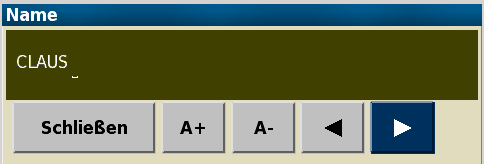
\includegraphics[angle=0,width=0.65\linewidth,keepaspectratio='true']{figures/textentry.png}
\end{center}

Um Text mit dem TouchScreen einzugeben, ist es sinnvoller  auf die "Tastatur"- bzw. Voreinstellung zu wechseln, einfach einen Buchstaben nach dem anderen mit der TouchScreen Tastatur eingeben (s.links).

In einigen Dialogen (z.B. beim Editieren und oder Eingeben \sketch{figures/textentry_keyboard.png}von Wegpunkten) schlägt \textsf{XCSoar} sofort den/die nächsten passenden Einträge aus der Datenbank vor bzw. unterdrückt nicht passende/nicht vorhandene Einträge, sodaß die Eingabe sehr schnell und komfortabel von sich geht.

Um den letzten Buchstaben zu löschen, drücke den  \button{$<-$} button.

Drücke auf  \button{Schließen} um die Eingabe zu übernehmen.

\section{Warntöne}\index{Warntöne}\index{Hinweistöne}

\textsf{XCSoar} erzeugt Geräusche für diverse Ereignisse, welche vom Bediener/Piloten  nach Belieben konfiguriert werden können.
Hierzu siehe~\ref{sec:status} für detaillierte Konfigurierung.

Wenn \textsf{XCSoar} an das VEGA-Variometer angeschlossen ist,  sendet \textsf{XCSoar} Kommando-Strings an das Subsystem des VEGA Sprachsystems, um von diesem Sprachausgaben und Warnungen erzeugen zu lassen, z.B.:

\begin{itemize}
\item Endanflug durch Gelände
\item Anfliegen/erreichen eines Wegpunktes
\item Luftraum Warnungen
\end{itemize}

\section{Bildschirmeinstellungen}

Es können einige Einstellungen der Bildschirmdarstellung und der Details auf \menulabel{\bmenut{Konfig.}{2/3}\blink\bmenus{System}}dem Bildschirm gewählt werden.  Der meistverwendet Punkt  ist hierbei wohl, ob die {\InfoBox}en weiß auf schwarz oder schwarz auf weiß - "invertierte Darstellung" genannt, dargestellt werden \menulabel{\quad\button{Aussehen}\blink\button{Anordnung}}sollen.  Einstellbar über \button{invertierte Infoboxen}. 

Die Einstellung der Helligkeit beim \al erfolgt entweder per \menulabel{\bmenut{Anzeige}{2/2}\blink\bmenus{Helligkeit}}Hardware gemäß des {\em \al User's Manual} oder aber wie links .  




\section{Hilfe System}
  Für die meisten Dialoge ist nun ein Hilfesystem vorhanden.
  Wenn eine Eigenschaft / ein Fenster \menulabel{\bmenus{Hilfe}} aufgerufen wurde, drücke auf den Hilfe-Knopf und eine entsprechender Hilfstext wird erscheinen, der die Auswahlmöglichkeiten  beschreibt. 

\section{Gestures}\label{sec:gestures}\index{Gesten}
Seit Version 6.0 unterstützt \textsf{XCSoar} auch sog.\  "Gesten".

Im Bild links wird angedeutet, wie man sich eine Geste vorzustellen hat. 
Es handelt sich hierbei um eine ganz normale Arbeitsweise, wie sie sie jeder kennt, der mit einem Touchscreen-Gerät
Für den normalen Bildschirm und für den \sketch{figures/gesture1.png} \fl-Bildschirm haben die Gesten unterschiedliche Bedeutungen, wie im  folgender Tabelle beschrieben wird. 
\newpage
 Wenn am Rande folgendes Icon \gesture{Hoch} erscheint, so bedeutet dies, daß für die beschriebene Funktion  die entsprechende Geste verfügbar ist. In diesem Falle  die Geste: ''Hoch''

%Eine Geste wird definiert als eine Bewegung von hoch, runter, rechts und links Bewegungen.
%Die Geste "LU"  z.B.\   steht hierbei für \gesture{Left-Up}.
%(Wenn am Rande der Seite das folgende Icon sichtbar ist, dann  stehen Gesten für die jeweilige Funktion zur %Verfügung.)

\textbf{Auf der Karte verfügbare Gesten:\index{Gesten! auf Karte}}

\begin{itemize}
 \item[\raisebox{-1em}{
\includegraphics[angle=0,width=0.1\linewidth,keepaspectratio='true']{figures/up.png}}] \p{Hoch}: Zoom herein 
 \item[\raisebox{-1em}{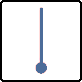
\includegraphics[angle=0,width=0.1\linewidth,keepaspectratio='true']{figures/down.png}}] \p{Runter}: Zoom heraus 
 \item[\raisebox{-1em}{
\includegraphics[angle=0,width=0.1\linewidth,keepaspectratio='true']{figures/left.png}}] \p{Links}: Nächste InfoboxSeite 
 \item[\raisebox{-1em}{
\includegraphics[angle=0,width=0.1\linewidth,keepaspectratio='true']{figures/right.png}}] \p{Rechts}: vorherige InfoboxSeite 
\item[\raisebox{-1em}{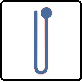
\includegraphics[angle=0,width=0.1\linewidth,keepaspectratio='true']{figures/du.png}}] \p{Runter-Hoch}: Menü anzeigen 
\item[\raisebox{-1em}{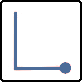
\includegraphics[angle=0,width=0.1\linewidth,keepaspectratio='true']{figures/dr.png}}] \p{Runter-Rechts}: Wegpunkt Dialog anzeigen 
\item[\raisebox{-1em}{
\includegraphics[angle=0,width=0.1\linewidth,keepaspectratio='true']{figures/rd.png}}] \p{Rechts-Runter}: Aufgabenverwaltung
\item[\raisebox{-1em}{
\includegraphics[angle=0,width=0.1\linewidth,keepaspectratio='true']{figures/urdl.png}}] \p{Hoch-Rechts-Runter-links}:  Verschiebemodus.  Dies geht aber auch  auch mit auf Android üblichem Spreizen oder Zusammenfahren von Zeigefinger und Daumen!
\end{itemize}


\textbf{Wenn das \fl-Radar auf dem Bildschirm aktiv ist, sind folgende Gesten verfügbar: }

\index{Gesten!FLARM Radar}
\begin{itemize}
\item[\raisebox{-1em}{
\includegraphics[angle=0,width=0.1\linewidth,keepaspectratio='true']{figures/up.png}}] \p{Hoch}: Zoom herein 
\item[\raisebox{-1em}{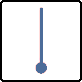
\includegraphics[angle=0,width=0.1\linewidth,keepaspectratio='true']{figures/down.png}}] \p{Runter}: Zoom heraus 
\item[\raisebox{-1em}{
\includegraphics[angle=0,width=0.1\linewidth,keepaspectratio='true']{figures/left.png}}] \p{Links}: Letztes Ziel (Flugzeug)
\item[\raisebox{-1em}{
\includegraphics[angle=0,width=0.1\linewidth,keepaspectratio='true']{figures/right.png}}] \p{Rechts}: Nächstes Ziel (Flugzeug)
\item[\raisebox{-1em}{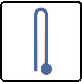
\includegraphics[angle=0,width=0.1\linewidth,keepaspectratio='true']{figures/ud.png}}]  \p{Hoch-Runter}: Aktiviere AutoZoom
\item[\raisebox{-1em}{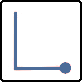
\includegraphics[angle=0,width=0.1\linewidth,keepaspectratio='true']{figures/dr.png}}] \p{Runter-Rechts}:  Öffne Detail-Fenster des gewählten Zieles (Flugzeuges)
\item[\raisebox{-1em}{
\includegraphics[angle=0,width=0.1\linewidth,keepaspectratio='true']{figures/rd.png}}] \p{Rechts-Runter}:  Öffnet die Aufgabenverwaltung
\item[\raisebox{-1em}{
\includegraphics[angle=0,width=0.1\linewidth,keepaspectratio='true']{figures/rl.png}}] \p{Rechts-Links}: Wechselt zur Anzeige von Werten wie z.B.\ Steigen, relativer Höhe etc.\ des angewählten Zieles (Flugzeuges) )
\end{itemize} 

%%%%%%%%%%%%%%%%%%%%%%
\chapter{Navegação}\label{cha:navigation}
Este capítulo descreve o mapa dinâmico e sua ajuda para a navegação, também descreve algumas informações de planeio e provas sobrepostas no mapa.

\section{Elementos mostrados no mapa}

\begin{maxipage}
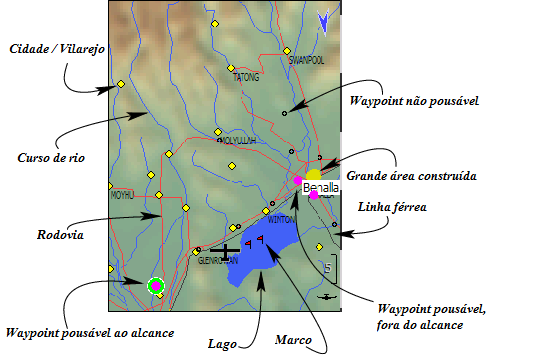
\includegraphics[angle=0,width=0.9\linewidth,keepaspectratio='true']{figures/fig-map.png}
\end{maxipage}

O mapa dinâmico mostra: 
\begin{enumerate} 
\item Aeronave, indicador de vento, perfil da termal, indicador de planeio final
\item Terreno, planícies e planaltos
\item Topografia, rios, rodovias e cidades
\item Waypoints, aeroportos e pousos
\item Prova ativa, zonas de observação e pilões
\item A direção (ou rota\footnote {A linha até o próximo waypoint pode ser uma {\em rota}, como descrição na seção~\ref{sec:route}.}) para a direção para o próximo waypoint.
\item Espaços aéreos
\item Marcadores, histórico de termais, trilha
\item Alcance do planeio\footnote{O alcance do planeio também é citado como
  {\em alcance}, assim como descrito na seção ~\ref{sec:reach}.}
\end{enumerate}
O mapa é desenhado em um sistema de coordenadas projetadas (sem latitude e longitude), e a escala pode ser alterada (zoom + e zoom -), bem como deslocado.  Todas as funções de navegação levam a curvatura da Terra em consideração.

\section{Símbolo do planador, orientação do mapa}
O símbolo do planador mostra a posição da aeronave no mapa.  A orientação da aeronave indica a direção estimada que a aeronave está apontando.

O mapa é orientado de três formas: norte acima, trilha acima e alvo acima.  O ajuste da configuração pode ser utilizado para especificar uma orientação diferente no mapa quando estiver em modo de círculos.  É bem útil para prevenir a desorientação quando olhar o mapa girando.  O modo alvo acima facilita determinar em qual direção se deve sair da termal.

Quando o modo trilha ou alvo acima é usado no modo de círculos, o símbolo da aeronave é centralizado na tela, mesmo que o símbolo seja configurado de outra forma.  No modo de cruzeiro, a orientação de trilha e alvo acima permite que o símbolo da aeronave seja posicionada (ex. 20\%) na parte inferior da tela, fornecendo uma boa visão do mapa à frente da aeronave.  Esta posição é definida nos ajustes da configuração.  

\section{Zoom e escala do mapa}\label{sec:zooming}

Para alterar a escala do mapa, dependendo do hardware, você usa:
\begin{enumerate}
\item Toque/clique em uma parte vazia do mapa para sublinhar o mapa se já não estiver selecionado.  Então utilize a roda do mouse ou as teclas acima/abaixo do Pocket PC para zoom + ou zoom -.
\item Um dispositivo PNA com um botão rotativo permite que se altere o zoom.
\item Dispositivos Android tem o +/- que permite que se altere o zoom.
\item Você pode também fazer o gesto para mudar o nível de zoom. Gesto acima (veja à esquerda) aumento o zoom.  Para baixo diminui o zoom.\gesturespec{up}
\item Ou selecione a função através do menu.
\begin{quote}
\bmenug{Mostrar 1}\blink\bmenug{Zoom In} e \bmenug{Zoom Out}
\end{quote}
\item No Altair, o botão rotativo pode ser usado para alterar o zoom.
\end{enumerate}

A escala do mapa é mostrada no canto inferior do mapa dinâmico.  A distância indicada é medida da borda esquerda para a direita do mapa dinâmico.
Usuários do Compaq Aero:  Se você ativar as teclas de jogo do Compaq Aero (no Menu-Q), os dois botões centrais serão as teclas acima/abaixo.
\marginpar{\includegraphics[angle=0,width=0.4\linewidth,keepaspectratio='true']{figures/zoom.png}}

Usuários do Compaq Aero:  Se você ativar as teclas de jogo do Compaq Aero (no Menu-Q), os dois botões centrais serão as teclas acima/abaixo.

\subsection*{Zoom Girando}
Há uma facilidade de ter dois tipos de zoom: um quando a aeronave está em modo girando e outro em modo de cruzeiro ou modo final.  Esta é a opção de Zoom girando, nos ajustes das configurações.  Por padrão, o zoom girando é ajustado em 2,5 – 5,0km dependendo do tamanho da tela.  Quando o usuário altera o zoom, afeta diretamente o zoom atual somente.  Quando se sai do modo atual de zoom, é usado o modo prévio de zoom. Se o modo de Zoom girando não está ativo, haverá somente um único nível de zoom.  Esta situação conduz a diferentes níveis de zoom sendo preservados para serem alterados manualmente, independentemente dos ajustes de Auto Zoom.
 
\subsection*{Auto Zoom}
Auto Zoom automaticamente aproxima a tela quando se está aproximando de um waypoint para manter a visualização em uma distância apropriada. 
\marginpar{\includegraphics[angle=0,width=0.4\linewidth,keepaspectratio='true']{figures/zoomauto.png}} 
Quando o Auto Zoom está ativo, ‘AUTO’ aparece perto da escala do mapa.

Para ativar o Auto Zoom, use o gesto \gesturespec{ud} ou o menu descrito à esquerda. Para voltar ao zoom normal, faça o zoom manualmente, não importando o que já foi feito por menu ou gesto. 

\menulabel{\bmenug{Mostrar 1}\blink\bmenut{Zoom}{Auto}}
Quando um waypoint muda (automaticamente, através do seletor de prova ou manualmente selecionando waypoints), o Auto Zoom ajusta o nível de zoom automaticamente para que o próximo waypoint seja visível no mapa.

Durante o modo Girando se uma termal foi detectada, o mapa é centrado sobre a termal ou parte dela para que a aeronave continue sendo visível.
 
\section{Navegando no mapa (Panning)}\label{sec:panning}

O modo panorâmico permite ao usuário explorar áreas que estão além da aeronave.  É bem útil quando se está planejando a prova.
\begin{enumerate}
\menulabel{\bmenug{Mostrar 1}\blink\bmenug{Pan On}}
\item Ative o modo panorâmico por menu ou gesto.  O gesto para este modo é mover sua ponta do dedo acima, direita, abaixo e esquerda, formando um “P”. 
\gesturespec{urdl}
\item O mapa pode ser movido arrastando a tela ou usando as teclas.  Para Altair, modo panorâmico é feito com o botão rotativo interno/externo.  
\item Quando feito, o modo panorâmico pode ser desabilitado manualmente, pressionando PAN OFF no sub-menu.
\end{enumerate} 

\sketch{figures/pan.png}
Quando o modo panorâmico está ativo, as letras ‘PAN’ aparecem próximas à escala do mapa.  Enquanto estiver nesse modo, o foco estará na mira no meio do mapa.

Apesar de aparecer a mira (para usuários Altair), o mapa continuará oferecendo a opção “Oque Aqui?” tocando em qualquer posição no mapa (na tela de toque). 


\section{Waypoints} \label{sec:waypoint-schemes}
Os waypoints são mostrados com símbolos diferentes, dependendo do tipo do waypoint; a maior diferença são waypoints pousáveis e não pousáveis.

\subsection*{Pousáveis}
Os símbolos dos waypoints são desenhados conforme abaixo.  Há três conjuntos de ícones disponíveis para waypoints pousáveis. \config{waypointicons}

\begin{tabular}{c|ccc|ccc|}
Conj. Ícones 
&\begin{sideways}Pousável\end{sideways}
&\begin{sideways}Marginal\end{sideways}
&\begin{sideways}Alcançável\end{sideways}
&\begin{sideways}Aeródromo\end{sideways}
&\begin{sideways}Marginal\end{sideways}
&\begin{sideways}Alcançável\end{sideways}\\
\hline
Círculo Roxo &
\includegraphics[width=0.8cm]{icons/winpilot_landable.pdf} &
\includegraphics[width=0.8cm]{icons/winpilot_marginal.pdf} &
\includegraphics[width=0.8cm]{icons/winpilot_reachable.pdf} &
\colorbox{white}{\includegraphics[width=0.8cm]{icons/winpilot_landable.pdf}} &
\includegraphics[width=0.8cm]{icons/winpilot_marginal.pdf} &
\includegraphics[width=0.8cm]{icons/winpilot_reachable.pdf} \\
\hline
Branco e Preto &
\includegraphics[width=0.9cm]{icons/alt_landable_field.pdf} &
\includegraphics[width=0.9cm]{icons/alt_marginal_field.pdf} &
\includegraphics[width=0.9cm]{icons/alt_reachable_field.pdf} &
\colorbox[rgb]{0.94,0.94,0.94}{\includegraphics[width=0.9cm]{icons/alt_landable_airport.pdf}} &
\includegraphics[width=0.9cm]{icons/alt_marginal_airport.pdf} &
\includegraphics[width=0.9cm]{icons/alt_reachable_airport.pdf} \\
\hline
Luzes de tráfego &
\includegraphics[width=0.9cm]{icons/alt2_landable_field.pdf} &
\includegraphics[width=0.9cm]{icons/alt2_marginal_field.pdf} &
\includegraphics[width=0.9cm]{icons/alt_reachable_field.pdf} &
\colorbox{white}{\includegraphics[width=0.9cm]{icons/alt2_landable_airport.pdf}} &
\includegraphics[width=0.9cm]{icons/alt2_marginal_airport.pdf} &
\includegraphics[width=0.9cm]{icons/alt_reachable_airport.pdf} \\
\hline
\end{tabular} \\

Os ícones marginais são desenhados para aqueles waypoints que estão principalmente no alcance, mas não é possível a aproximação direta (ex. uma montanha não permite a aproximação direta).
  
Os waypoints são rotulados opcionalmente de acordo com suas abreviações, esquemas e visibilidade.

No topo dos waypoints pousáveis, pode haver mais detalhamento.  Se houver a opção ativada 
`{\it Detalhar Pousáveis}' você terá informações adicionais quando houver a visualização deste waypoints.

\begin{enumerate}
\item  Campos pousáveis têm ícone quadrado apesar de serem mostrados em tabela.  O quadrado é desenhado como um diamante em pé.  Aeródromos permanecem com um círculo, facilitando sua visualização. 
\item  Todo o conjunto de ícones, incluindo o conjunto de “círculos roxos”, colocam a pista em suas atuais direções.  A direção da pista está disponível nos dados do waypoints.  Ex. os waypoints de formato (\verb|.cup|) não incluem esta informação.
\end{enumerate}

\subsection*{Pousáveis ao Alcance}
Próximo aos pousáveis, há uma estimativa da altitude acima da altura de segurança dos pontos pousáveis e é mostrada próxima ao waypoints.  Esta característica é uma das capacidades mais poderosas do XCSoar.  A altitude de chegada é calculada configurando-se o computador de planeio do XCSoar com parâmetros de polar, ajustes de MacCready, vento, abertura do terreno e altitudes de segurança.  Com tudo isso sendo configurável, há muito espaço para erros, portanto:

A menos que tenha entendido completamente os conceitos de cálculo de planeio, você deve \warning manter a pré-configuração do XCSoar (já julgado e fortemente aprovada).

É da responsabilidade do piloto sempre interpretar a leitura e observar os valores com o tempo.  Todavia, tendo ajustado o computador de planeio seguindo o Capítulo 
\ref{cha:glide} mostra a altitude estimada de alcance, desenhada ao lado de campos pousáveis ao alcance levam em consideração o relevo ou mostram ambos.
\config{arrivalheight}

Outra opção é mostrar o planeio médio necessário para um campo pousável ao alcance.  Este cálculo é derivado da distância atual ao campo pousável dividido pela diferença de altura entre a altura atual e a altura do campo pousável.  Novamente, a altura de segurança é adicionada à altura do campo pousável, mas nada mais é levado em consideração: sem vento, sem polar, sem ajuste MacCready, só geometria.  O conceito do planeio médio necessário é amplamente discutido, como um conceito bem robusto.

\tip Tenha em mente que necessita de um forte conhecimento dos dados de alcance e ajustes no computador de planeio.

\subsection*{Não Pousáveis}
Como o arquivo de waypoints contém informações da natureza do campo não-pousável, o mapa mostrará ícones específicos para estes pontos.  A tabela contém uma relação dos ícones de mapas apresentados (veja figura  \ref{fig:nonlandables}).

\begin{figure}[h]
\centering
\vspace{2.5cm}
\begin{tabular}{ccccccccc}
\begin{rotate}{60}Waypoint simples\end{rotate} &
\begin{rotate}{60}Topo da montanha\end{rotate} &
\begin{rotate}{60}Obstáculo\end{rotate} &
\begin{rotate}{60}Passagem\end{rotate} &
\begin{rotate}{60}Planta ou fábrica\end{rotate} &
\begin{rotate}{60}Torre ou prédio\end{rotate} &
\begin{rotate}{60}Túnel\end{rotate} &
\begin{rotate}{60}Estação metereológica\end{rotate} &
\begin{rotate}{60}Ponte\end{rotate}\\

\includegraphics[width=0.5cm]{icons/map_turnpoint.pdf} &
\includegraphics[width=0.8cm]{icons/map_mountain_top.pdf} &
\includegraphics[width=0.7cm]{icons/map_obstacle.pdf} &
\includegraphics[width=0.7cm]{icons/map_pass.pdf} &
\includegraphics[width=0.8cm]{icons/map_power_plant.pdf} &
\includegraphics[width=0.7cm]{icons/map_tower.pdf} &
\includegraphics[width=0.6cm]{icons/map_tunnel.pdf} &
\includegraphics[width=0.6cm]{icons/map_weather_station.pdf} &
\includegraphics[width=0.8cm]{icons/map_bridge.pdf} \\

\end{tabular}
\caption{não pousáveis}\label{fig:nonlandables}
\end{figure}

\section{Prova ativa}

O curso da prova ativa é desenhado no mapa em linha azul (pontilhada).  As áreas atribuídas às provas mostram os setores dos pilões ou áreas sombreadas em amarelo.  Círculos são desenhados ao redor dos pontos de início e fim, as linhas são desenhadas nos pontos de início e fim se os pontos são deste tipo.  Os setores de observação da prova são desenhados em segmentos de círculos.

A todo tempo, uma linha fina é desenhada da aeronave até o próximo waypoint da prova.  Esta linha deve ser um caminho direto ao waypoint, ou ser uma rota livre de terrenos e espaços aéreos, descritos anteriormente em detalhes na seção
~\ref{sec:route}.

\begin{center}
\begin{tabular}{c c c}
{\it Início/Fim} & {\it Setor} & {\it Cilindro} \\
\includegraphics[angle=0,width=0.3\linewidth,keepaspectratio='true']{figures/cut-startfinish.png} &
\includegraphics[angle=0,width=0.3\linewidth,keepaspectratio='true']{figures/cut-sector.png} &
\includegraphics[angle=0,width=0.3\linewidth,keepaspectratio='true']{figures/cut-barrel.png} \\
\end{tabular}
\end{center}


\section{Terreno e Topografia}\label{sec:terrain_topo}

As seguintes características de topografia são desenhadas no mapa:
\begin{itemize}
\item Rodovias principais, mostradas em linhas vermelhas
\item Rios, mostrados em linhas azuis
\item Grandes corpos de água (lagos), mostrados em áreas azuis
\item Cidades grandes, mostradas em áreas amarelas
\item Áreas de pequena população, mostrada como diamantes amarelos 
\end{itemize}
Cidades e pequenas áreas com população são rotuladas em itálico.

O solo é colorido de acordo com a elevação e opcionalmente sombreado pelo sol ou pela direção do vento.  Solos inválidos ou abaixo do nível do mar são coloridos em azul.


\menulabel{\bmenug{Mostrar 2}\blink\bmenut{Terreno}{On/Off}}
\menulabel{\vspace{1cm}\bmenug{Mostrar 2}\blink\bmenut{Topo.}{On/Off}}

O solo é sombreado para melhorar a visibilidade.  O sombreamento padrão é ajustado coincidindo a iluminação virtual com a direção do vento, sendo as áreas mais brilhantes são barlavento e as áreas mais escuras são sotavento.   
A inclinação solar também foi implementada.  Se o sombreamento da encosta for ajustado para ‘Sol’, o brilho da encosta segue conforme o dia e hora.  A quantidade de sombra sobre o brilho do terreno é ajustável \config{shading}.

A visualização do solo e topografia podem ser acionados ou não através do menu.

\begin{tabular}{c c}
Topografia & Terreno \\
\includegraphics[angle=0,width=0.4\linewidth,keepaspectratio='true']{figures/cut-topo.png} &
\includegraphics[angle=0,width=0.4\linewidth,keepaspectratio='true']{figures/cut-terrain.png} \\
\end{tabular}

Se os dados do solo não estiverem disponíveis (ou a visualização estiver desligada), a cor de fundo do mapa será branca.  Todo o solo abaixo do nível médio do mar é mostrado em azul.  Se você estiver voando fora da terra, o fundo da tela será branco.  

\subsection*{Rótulos do mapa}\label{sec:maplabels}

A tela pode ser mais clara desligando a visualização dos rótulos de topografia e waypoints for a da prova escolhendo o menu ‘Rótulos’.
\menulabel{\bmenug{Mostrar 2}\blink\bmenut{Rótulos}{Nenhum}}

Outra opção para deixar mais clara incluem:

\jindent{\bmenuth{Rótulos}{Prova \&}{locais pouso}}{  Mostra rótulos para os waypoints na prova ativa e campos pousáveis (baseado nos atributos dos waypoints).  Os outros waypoints serão mostrados, mas sem rótulos. }

\jindent{\bmenut{Rótulos}{Prova}}{ Mostra somente os rótulos dos waypoints da prova ativa.}
\jindent{\bmenut{Rótulos}{Todos}}{ Mostra todos os rótulos para todos os waypoints.}

Note que em todos os casos, a formatação dos rótulos é configurável no menu
`{\it Waypoint Display}'.  \config{labels}


\section{Rastro}\label{sec:trail}


Um rastro opcional pode ser desenhado no mapa dinâmico para mostrar o caminho da aeronave.  A cor e a espessura do rastro dependem de altitude ou do valor do variômetro.


\begin{center}
\includegraphics[angle=0,width=0.5\linewidth,keepaspectratio='true']{figures/snail.pdf}
\end{center}

Se houver conexão do Vega ou outro variômetro inteligente com a saída Netto, o valor do vário Netto é usado; conseqüentemente as cores e a espessura do rastro indicarão o movimento vertical da massa de ar ao invés do movimento vertical da aeronave.

\config{snailtrail}
A visualização do rastro pode ser ajustada entre Desligado, Curto (+/- 10 minutos), Longo (+/- uma hora) ou Completo que mostrará todo o vôo.  Isto pode ser ajustado através dos ajustes de configuração ou temporariamente através do menu.
\menulabel{\bmenug{Mostrar 2}\blink\bmenut{Trilha}{Completo}}

Observe que para todos estes modos, o rastro é curto no modo Girando para facilitar a visualização.

De modo a auxiliar a centralização das térmicas na presença de vento, o rastro pode ser artificialmente derivado com o vento conforme vai sendo mostrado (é a compensação de deriva).  Deste modo, o rastro é referenciado pelo vento e não pelo solo.  Assim como as termais também são derivadas com o vento, o rastro pode dar uma indicação mais precisa onde esteve a aeronave com relação às termais.

O exemplo é ilustrado abaixo.  Observe que, quando a compensação da deriva do vento está ativa (figura à direita), a aeronave aparenta estar girando em uma coluna ao invés de estar em uma espiral alongada (figura à esquerda).

\begin{center}
\includegraphics[angle=0,width=0.6\linewidth,keepaspectratio='true']{figures/traildrift.png}
\end{center}

\config{traildrift}
Ativando a compensação da deriva do rastro é através dos ajustes de no menu de configuração. A compensação só é feita no modo Girando; a visualização do rastro no modo Cruzeiro não é afetada.  Também pode ser alterada pela janela de ajuste do vento.
\menulabel{\bmenug{Config 1}\blink\bmenus{Vento}}

A visualização do rastro é útil também para mostrar mais claramente quando as termais são cisalhadas pelo vento.
A largura da trilha pode ser opcionalmente alterada de acordo com a visualização do variômetro.  


\section{Marcadores}\label{sec:markers}

Os marcadores são mostrados como pequenas bandeiras no mapa.  Os marcadores podem ser adicionados manualmente ou automaticamente.  Um exemplo de como estes marcadores podem ser adicionados automaticamente é quando se entra em modo Girando, um modo simples de mostrar as termais encontradas.

\menulabel{\bmenug{Nav 2}\blink\bmenut{Marca}{Ponto}}
Os marcadores não são mantidos após o XCSoar ser fechado, porém a localização dos marcadores é anexada ao arquivo
 \verb|xcsoar-marks.txt|.

\section{Termais}

Enquanto estiver girando em termais, automaticamente será gerado um marcador e mantido até o \sketch{figures/thermalhistory.png} fim do vôo.  Este histórico termal é acessível através da função de elementos de mapa, da mesma forma que os marcadores ou waypoints.


\section{Linha de alcance de planeio}\label{sec:reach}

Uma linha de alcance de planeio é mostrada no mapa como uma linha pontilhada branca e preta, indicando onde a aeronave poderá pousar em terreno aberto.  O alcance é mostrado em todas as direções, incluindo caminhos obstruídos no terreno.  Esta opção é útil para conhecer o planeio relativo à topografia quando se está baixo e procura por termais, ou quando está voando em áreas montanhosas.

Os cálculos para o alcance podem ser configurados \config{turningreach} em dois níveis: 
\begin{description}
\item[Linha reta] se o alcance em curva está desabilitado, mostrará a maior distância que a aeronave pode voar no planeio final em todas as direções sem fazer curvas.  O alcance aparece como um anel fechado ao redor da aeronave.  

\begin{center}
\includegraphics[angle=0,width=0.8\linewidth,keepaspectratio='true']{figures/reach1.png}
% CUTOUT SHOWING GLIDE RANGE FOOTPRINT.  NO TOPOGRAPHY, FULLSCREEN, NO TASK. TURNING=FALSE
\end{center}

\item[Girando] se o modo Girando estiver ativo, o planeio será mostrado como a maior área que a aeronave pode alcançar em todas as direções, mesmo permitindo curvas ao redor de obstáculos.  A área de alcance aparece com um anel fechado ao redor da aeronave mas também pode incluir buracos indicando picos de montanhas que a aeronave não pode alcançar sem subir.

\begin{center}
\includegraphics[angle=0,width=0.8\linewidth,keepaspectratio='true']{figures/reach2.png}
% CUTOUT SHOWING GLIDE RANGE FOOTPRINT.  NO TOPOGRAPHY, FULLSCREEN, NO TASK. TURNING=TRUE
\end{center}

\end{description}

A tela pode ser configurada também para desfocar as áreas não alcançáveis fora do alcance do planeio da aeronave.  O caminho do planeio final é verificado levando-se em consideração também a abertura do terreno através do caminho e também a altura do terreno.
Se a abertura (clareza) do terreno não é atingida, aparecerá uma cruz vermelha no mapa onde a área é perigosa.  Se um alvo for definido, os cálculos são feitos através do caminho reto para o alvo.  Se não há alvo definido, o cálculo é feito através do caminho que está seguindo.
Se o alcance estiver ativo, o modo de aborto de prova usará os waypoints pousáveis e abrirá uma lista também com os waypoints alternativos do mapa.
Observe que os cálculos da prova não são afetados pelos cálculos de alcance – por exemplo, não são levados em conta os dados de altitude necessária para finalizar a prova e dados mostrados nas infoboxes.

Além do mais, os cálculos são usados para o anel de alcance, altura de chegada para waypoints pousáveis, modo de aborto e janelas de diálogo alternativas.  O desempenho da aeronave e os ajustes de MacCready usados nestes cálculos são configuráveis\config{reachpolar}:
\begin{description}
\item[Prova] O valor de MC é o usado na prova.
\item[Safety MC] Um valor de MC baixo pode ser configurado para ser usado como referencial ao melhor planeio da aeronave.  O grau de segurança alcançado nos cálculos é feito com a diferença entre o melhor desempenho de planeio e o planeio seguindo o MacCready de Segurança (speed to fly).  
\end{description}

\section{Abas de estado `{\it Voo}' e `{\it Tempo}'}\label{sec:flight-status}

A janela de diálogo Estado é multi-tabular, fornecendo uma visão geral da informação do vôo, sistema, prova, regras e tempos.  Pode ser acessada com o gesto “S” ou com o botão do Menu. 
\gesture{Esquerda - Baixo - Direita - Baixo - Esquerda}
\begin{quote}
\bmenug{Info 2}\blink\bmenug{Estado}
\end{quote}

\subsection*{Vôo}
Selecione a página `{\it Flight}'. 
A janela mostra a localização da aeronave e pode ser útil quando se reporta a posição.  Mostra a posição da aeronave, o máximo ganho de altura, waypoints mais próximo, ângulo de direção e distância.
\sketch{figures/status-flight.png}

Você pode achar esta função útil quando for reportar sua localização para outros pilotos ou resgate.

\subsection*{Tempo}\label{sec:time-status}
Seleciona a aba  `{\it Times}'. 
Mostrará a hora local, tempo de vôo, hora da decolagem e pouso e hora do nascer e pôr do sol.

Observe que estes valores nesta aba são estáticos e só serão atualizados a cada abertura de aba. 
\sketch{figures/status-times.png}
Para ver os dados atualizados, é necessário fechar a aba e abrí-la novamente.  Os valores serão atualizados automaticamente a cada abertura desta janela.  Familiarize com este procedimento antes de realizá-lo em vôo.


\section{Rota}\label{sec:route}

O XCSoar pode planejar caminhos pelo terreno e obstáculos no espaço aéreo em três dimensões da aeronave até o destino.  Este caminho é conhecido como rota.  A altura do destino é a altura de chegada para waypoints finais ou pode ser mais alto para waypoints intermediários, se forem regras da prova ou requisitos para completar a prova.  

As funções de planejamento de rota são ordenadas por modo de prova, modo de aborto e modo ‘ir para’.

\begin{center}
\includegraphics[angle=0,width=0.8\linewidth,keepaspectratio='true']{figures/route3.png}
\end{center}

As rotas levam em consideração o desempenho da polar e são calculadas para levarem o mínimo tempo.  Por padrão, os cálculos de rota são desativados e podem ser ativados somente por solo ou quando na prevenção de espaço aéreo. \config{routemode}

O solo é evitado verticalmente pela altura de segurança do terreno \config{safetyterrain}, sem nenhuma abertura de terreno lateral.  As rotas válidas podem  resultar na chegada da aeronave ao destino mais alta que a altura mínima – como pode ocorrer quando o destino está além de uma montanha mais alta.

O espaço aéreo é evitado horizontalmente por uma margem de aproximadamente 250m sem nenhuma abertura imposta verticalmente.  As rotas válidas podem voar acima ou abaixo do espaço aéreo.

Se o MacCready é positivo, a subida é opcionalmente permitida nos cálculos de rota.  O topo da subida deve ser limitado a 500m acima do teto de início e final, ou incluso no teto, definido pelo teto da termal \config{routeceiling}.  As subidas acima da altitude de início e final são penalizadas por uma taxa de subida mais lenta que o valor de MacCready atual.

Algumas aproximações e limitações do sistema de planejamento de rotas são:
\begin{itemize}
\item Quando subidas são necessárias (e permitidas) para alcançar o destino, as subidas podem ocorrer no início da rota. 
\item Segmentos de subidas em cruzeiro podem ocorrer em altitude constante, equivalente a muitas pequenas subidas distribuídas ao longo do caminho. 
\item Falhas sobre o resultado dos cálculos podem se reverter em vôo direto da aeronave, de sua localização atual para o destino.
\end{itemize}



%%%%%%%%%%%%%%%%%%%%%%
\setcounter{chapter}{4}
\chapter{Überlandflug Aufgaben - Navigieren mit\textsf{XCSoar}}\label{cha:tasks}
\index{Aufgabe}\index{Tasks}

\textsf{XCSoar} bietet ein ausgefeiltes, komplettes Aufgabenmanagementsystem, mit dem Aufgaben vor und während des Fluges erstellt, editiert und auch gelöscht werden können.

Die Wendepunkte können vollautomatisch angeflogen und umgestellt werden, wobei die Kartendarstellung automatisch hinein- bzw. herausgezoomt werden kann. Ein rein manuelles  Anwählen und Umschalten ist aber ebenso möglich.

Dieses Kapitel beschreibt weiterhin die Benutzung von \textsf{IGC} Loggern mit\textsf{XCSoar}

Intern werden drei Aufgabentypen (modi)  unterschieden
\begin{description}
\item[\p{Deklarierte Aufgabe}] Dies ist der eigentliche Überlandflug-Modus, bei dem ein Startpunkt, ein
    Zielpunkt und mehrere Wendepunkte deklariert sein können. Die Wendepunkte müssen in der
    angegeben Reihenfolge angeflogen werden. (Leistungsflug)\index{Task!Leistungsflug}
\item[\p{''Ziele auf''-- Aufgabe}] Ein Flug auf exakt ein einziges Ziel zu. (Irgendein Flug)\index{Task!Zielflug}
\item[\p{Abort - Aufgabe}] Hier wird "frei" durch die Gegend geflogen, ohne einen Wegpunkt als  Ziel
    deklariert zu haben. (Lustflug)\index{Task!Lustflug}
\end{description}

 Beachte, daß im ''Ziele auf''- und im Abort - Modus  die  evtl.\ abgebrochene Aufgabe \textsl{jederzeit} wieder \tip aufgenommen werden kann, dies unter Beibehaltung sämtlicher bisher aufgenommenen Berechnungen und Statistiken.

\section{''Ziele auf''-- Aufgabe}\index{Aufgabe!''Ziele auf'-'-Typ}\index{Task!''Ziele auf''}

''Ziele auf''--Aufgaben'' können erstellt werden, indem man einen Wegpunkt auf der Karte markiert und anschließend auf dem ''Kartenelemente an diesem Ort'' oder dem Wegpunkt-Detailfenster mit "Ziele auf" bestätigt.  Alternativ kann auch über den "Alternative" Dialog zu einem Wegpunkt gelangt werden, welcher anschließend mit ''Ziele auf'' festgelegt wird.

Während des ''Ziele auf''--Modus \menulabel{\bmenut{Nav}{2/2}\blink\bmenut{Aufgabe}{fortsetzen}} kann eine vorher abgebrochene Aufgabe immer wie links fortgesetzt werden.

\subsection{Automatik ''Ziele auf''}\index{Automatik--''Ziele auf''}\index{Heimatflugplatz!Automatik}

Wenn keine deklarierte Aufgabe geladen ist, dann wird nach dem Start unverzüglich in den ''Ziele auf''--Modus geschaltet. Hierbei wird der Startplatz oder aber (falls es z.B. eine Wiese war, von der man mit einer Wilga im F-Schlepp gestartet ist), der nächstgelegene landbare Flugplatz automatisch als Ziel in den Rechner eingefügt.

Egal, ob eine Aufgabe deklariert wurde, oder nicht, es wird grundsätzlich ein Startpunkt erfaßt, welcher für spätere Benutzung während des Fluges in der Wegpunktliste erscheint und ganz normal  verwendet werden kann. 
Dieser Punkt ist auf der Karte als ''take-off' gekennzeichnet' \todonum{wird der auch gespeichert? wo ?}

\section{Aufgaben erstellen und bearbeiten}\index{Aufgabe!Erstellen}\index{Aufgabe!Bearbeiten}

Aufgaben können auf unterschiedliche Weise erstellt und editiert  werden. Manche Methoden eigentlich mehr für die Bearbeitung und Erstellung vor dem Flug,  andere erlauben es eine Aufgabe während des Fluges zu ergänzen bzw. zu verändern.

Aufgaben können in Dateien (Files) gespeichert werden um später geladen zu werden oder aber um zwischen verschiedenen Geräten hin und her kopiert zu werden. Alle\textsf{XCSoar} Plattformen sind Dateiformatskompatibel d.h.\  jede Aufgabe kann auf jedem\textsf{XCSoar} erstellt, geflogen und gespeichert werden. (\textsf{Pocket PC, Altair, PC, Android, MAC)}).

\tip Es ist möglich (und sinnvoll) eine Standard-Aufgabe zu erstellen und zu speichern und diese  Aufgabe beim jedem Start von\textsf{XCSoar} automatisch laden zu lassen.

Eine Anwendung dieser Standardaufgabe ist zum Beispiel, einen Wegpunkt  als Heimatflughafen zu deklarieren. d.h.,  der Heimatflugplatz ist anschließend grundsätzlich automatisch als Ziel eingestellt, wenn man einfach nur durch die Gegend fliegen will.

Die Möglichkeiten, Aufgaben zu erstellen sind wie folgt:
\begin{itemize}
\item Benutzen des Aufgabeneditor-Dialogs
\item Auswählen eines Wegpunktes von der Karte und hinzufügen zur Aufgabe über den Wegpunkt Detail-Dialog.
\item Laden einer Aufgabe aus einer Datei.
\end{itemize}

\tip Aufgaben in einer Datei zu sichern und anschließend wieder zu laden ist sehr sinnvoll,  will man zum Beispiel mit mehreren Piloten eine gleiche Aufgabe fliegen oder aber im Wettbewerb ist, wo im  allgemein die Aufgaben vorher deklariert und eingegeben werden.

Entscheidend hierbei ist, daß lediglich eine Person die Aufgabe eingeben muß und diese anschließend  per copy \& paste,  Bluetooth oder Kabel kopiert werden kann.

\textsf{XCSoar} sichert die aktuelle Aufgabe beim Herunterfahren und lädt die gleiche Aufgabe wieder beim Neustart.  Die Wegpunkte einer Aufgabe sind sogar gesichert, wenn die Wegpunktdatei gewechselt wird. d.h., wenn eine Aufgabe gespeichert wird, anschließend das Wegpunktfile gewechselt wird, die gleiche Aufgabe wieder geladen  wird, wenn die Wegpunkte, welche in der Wegpunktdatei  fehlen automatisch durch die Wegpunkte aus der Aufgabe ergänzt.

\section{Wegpunkt Info und Details }\index{Wegpunkte!Details}

Der Wegpunkt-Info-Dialog beschreibt die Details der Wegpunkte  und bietet Navigations-Optionen wie zum Beispiel \textsf{Ziele auf}, \textsf{Einfügen} oder \textsf{Anhängen} an einer Aufgabe. Weiterhin kann über diesen Dialog ein Wegpunkt als Heimatflughafen eingegeben werden.

Die Anwahl  kann über mehrere Wege erfolgen:
\begin{itemize}\itemsep=1em
\item
Über die Karte, wenn der Wegpunkt sichtbar ist: \\
Ein \textit{einfacher} Klick öffnet das "Kartenelemente an diesem Ort''-Fenster.

Anschließend auf \button{Details} drücken.
%
%
\item
Über das Menü
\begin{quote}
\button{Nav}\blink\button{Alternativen}, Auswahl des Punktes und \button{Details}
\end{quote}
%
%
\item Über den Aufgabeneditor: \index{Wegpunkte!Anwahl}
\begin{quote}
\button{Nav}\blink\button{Aufgabe}\blink\button{Wendepunkte}\blink\button{Wendepunkt  hinzufügen}, Auswahl des Punktes und \button{Details} oder Doppelklick 
\end{quote}
%
%
\item%[\Large{$\bullet$}]
Vom Wegpunkt-Auswahlmenü \button{Nav}\blink\button{Wegpunkt Liste} und \button{Auswählen}
(Hier kann mittels eines einiger Filters besonders schnell und elegant jeder beliebige Wegpunkt auf schnellstmögliche Weise ausgewählt werden. Sehr effektiv, wenn man nicht nur den nächst möglichen Wegpunkt anwählen will.)
%
%
\end{itemize}

Der Wegpunktdetail-Dialog enthält zwei maßgebliche Seiten, welche über \button{$>$} und  \button{$<$} weiterschaltbar sind. Je nach dem, ob noch weitere Informationen zum Wegpunkt vorliegen, erscheinen Seiten mit weitere Details hierzu.

Auf dieser Seite werden Details zum Wegpunkt wie z.B.\ Funkfrequenz, Länge der Bahn, Höhe, Art der Bahn, Namen, Peilung (Bearing), Sonnenuntergang Entfernung zum Wegpunkt. etc.\ angegeben.

Zusätzlich befindet sich ein Button \button{Fliege Zu} um direkt zu diesem Punkt zu navigieren.  Dieser Button brichtt die aktuelle Aufgabe, sofern vorhanden, ab.

\sketch{{figures/dialog-waypointdetails0.png}}
Wie bereits oben erwähnt, zeigt der Wegpunkt-Info-Dialog drei Höhendifferenz-Angaben zum Erreichen des Wegpunktes, welche hier unten beschrieben werden:

\begin{description}
\item[\p{Ortskoordinaten}] Die Koordinaten des Punktes in Grad, Minuten und Sekunden
\item[\p{Höhe}] Die Höhe (MSL) des Punktes
\item[\p{Tageslichtzeiten}] Sonnenauf- und Untergang
\item[\p{Peilung und Distanz}] Richtung und Entfernung zum Punkt
\item[\p{H Diff MC 0}] Benötigte Höhe bei MacCready Null
\item[\p{H Diff MC sicher}] Benötigte Höhe bei Sicherheits MacCready (s. Kap~\ref{sec:safety-factor})
\item[\p{H Diff MC aktuell}] Benötigte Höhe bei  aktuell eingestellten MacCready Wert
\end{description}

Über die Buttons \button{$<$} und \button{$>$} in der linken unteren Ecke des Fensters können weitere Seiten mit Informationen über den aktuellen Wegpunkt angewählt werden. Weiterhin wird damit ein Menü geöffnet, auf dem z.B. dieser Wegpunkt als Ziel, Heimat oder Aufgabenwegpunkt eingefügt werden kann.


\subsection*{Flugplatz Informationen}
Diese Seite kann -sofern Daten zum Flugplatz vorhanden- etliche Hinweise und Details zu Flugplätzen enthalten. \sketch{figures/dialog-waypointdetails1.png}
Insbesondere sind hier enthalten Details zur Landebahn, Landebahnrichtung, Höhe, Frequenz usw.


\subsection*{Satelliten Photo}
Sofern vorhanden, kann hier z.B.\ ein Foto des Flugplatzes eingefügt und angezeigt werden. 
Näheres hierzu siehe Kap.~\ref{sec:airfield-details} 


\section{Wegpunkt-Auswahl-Dialog}\label{sec:waypoint-selector-dialog}
Der Wegpunkt-Auswahl-Dialog ist \textsl{der} Dialog, von dem aus Wendepunkte die in einer Datenbank (Datei) \menulabel{\bmenut{Nav}{1/2}\blink\bmenut{Wegpunkt}{Liste}}enthalten sind, ausgewählt werden kann.

Die Wegpunktlisten-Auswahlseite bietet einen Satz an von vier Filtern, um die Auswahl der entsprechenden \gesture{Runter -Rechts} Wegpunkte schneller und effizienter zu machen. Diese Filter können einzeln, gar nicht oder alle zusammen benutzt werden, umso die Auswahl eines Wegpunkt  einzugrenzen.

Folgende Wegpunktfilter sind vorhanden:

\begin{description}
\item[\p{Name}] Dieser Filter bietet eine sehr schnelle Möglichkeit, Wegpunkte anhand des Namens herauszufiltern.
\item[\p{Distanz}] Über diesen Filter werden die Wegpunkte nach der Entfernung angeordnet. Die nächstgelegene 
Mittelpunkte werden an die Spitze der Liste gesetzt.
\item[\p{Typ}] Über diesen Filter werden die Wegpunkte anhand ihrer Eigenschaft (Flugplatz, Landefeld, Startpunkt, oft benutzt, enthalten im Wegpunktdatei 2), usw. ausgewählt.
\item[\p{Richtung}] Hiermit werden Wegpunkt ausgewählt, welche in der entsprechenden gewünschten Richtung liegen. Ein besonderer Filter hierbei ist der Heading-Filter (\textsf{HDG(0$^\circ$)}) welcher nur Wegpunkte anzeigt, die sich in einem Winkel von $\pm 30\circ$ zur Flugrichtung befinden.
\end{description}

Wenn die Filterung nach Namen und gilt gewählt wird, ist die Ergebnisliste nach dem Namen geordnet. Wenn (auch zusätzlich) die Wegpunkte nach Entfernung oder Richtung gefiltert werden, dann erfolgt die Sortierung der Wegpunkte grundsätzlich als erstes nach der Entfernung.
D.h., der als nächste gefundene Wegpunkt wird immer an die Spitze der Liste gesetzt.

\sketch{figures/dialog-waypointselect.png}
Diese Ergebnisliste kann durchgescrollt werden, wenn Sie Einträge mehr als auf einer Seite dargestellt werden können. Um zu scrollen, einfach mit dem Finger auf dem TouchScreen hoch und runter, oder aber die Drehknöpfe beim Altair benutzen, alternativ mit der Maus ans Ende oder Spitze der Liste fahren.

Je nachdem aus welcher Situation die Wegpunktauswahl aufgerufen wurde, kann das Verhalten unterschiedlich sein. Normalerweise bringt die Anwahl eines Wegpunktes aus der Liste  direkt das Wegpunkt-Detail-Fenster.

\section{Aufgabenverwaltung }\label{sec:task-manager-dialog}
Die Aufgabenverwaltung wird benutzt, um Aufgaben zu erstellen, zu löschen, zu \menulabel{ \bmenut{Nav}{1/2}\blink \bmenus{Aufgabe}}speichern und zu deklarieren. 
Sie ist in der Zwischenzeit massiv überarbeitet und komplett neu gestaltet worden.

Gegenüber früheren Versionen von \textsf{XCSoar} befindet sich so gut wie nichts mehr an der gewohnten und üblichen Stelle. 

Das Arbeiten mit der neuen Version hat sich jedoch erheblich vereinfacht und ist deutlich komfortabler, übersichtlicher und schneller geworden.

Die Startseite der Aufgabenverwaltung ist der Rechner. Hier werden diverse berechnete Werte angezeigt, die \menulabel{\includegraphics[keepaspectratio,width=0.4\textwidth]{figures/dialog-taskcalculator.png}}aktuelle Aufgabe betreffen und im Detail weiter unten beschrieben werden.

Weiterhin stehen folgende Buttons zur Verfügung:

  \p{Rechner}, \p{Wendepunkte}, \p{Verwalten}, und \p{Regeln}, sowie selbstverständlich \p{Schließen}, um die Aufgabenverwaltung zu schließen.

\subsection*{Wendepunkte}
Der Button  \button{Wendepunkte} zeigt eine Liste der aktuell in der jeweiligen Aufgabe bestimmten Wegpunkt. Wenn kein Wegpunkt In der aktuellen Aufgabe gelistet ist, gibt es nur eine einzige Option, und zwar die, einen Wegpunkt hinzuzufügen: "Wegpunkt hinzufügen"

Durch Drücken auf die graue "Wendepunkt hinzufügen" Schaltfläche wird die Wegpunkt Auswahl gestartet (siehe
oben).  Ein hier ausgewählter Wegpunkt erscheint anschließend in der Aufgabe.

\subsection*{Verwalten}
Durch Drücken auf den Button \button{Verwalten} wird die Verwaltung der Aufgaben geöffnet, hierbei erscheinen vier große Schaltflächen:

\begin{itemize}
\item \button{Neue Aufgabe} Löscht die aktuelle Aufgabe und setzt die Regeln auf die Standardwerte.
\item \button{Anmelden} Wenn ein externer Bürger angeschlossen ist, wird hiermit die aktive Aufgabe an den Logger übertragen und somit deklariert.
\item \button{Durchsuchen} Zeigt eine Liste aller gespeicherten Aufgaben, und erlaubt es, Aufgaben zu laden. Beachte, daß diese Option die aktuelle Aufgabe löscht.
\item \button{Speichern} Sichert die aktuelle Aufgabe. Nachdem die Schaltfläche berührt wurde, wird der Not aufgefordert, einen Namen zu vergeben, unter dem die Aufgabe gespeichert wird und wieder geladen werden kann.
\end{itemize}

\subsection*{Regeln}\index{Regeln}
Die Werte, die bei Anklicken des Buttons \button{Regeln} erscheinen, hängen vom Typ der Aufgabe ab, die vorher erstellt wurde.

Durch Anklicken der jeweiligen weiß hinterlegten Werte wird ein Untermenü geöffnet, auf dem diese Werte entsprechend geändert werden können. Die diversen Aufgabentypen werden in einem Abschnitt weiter unten besprochen.

Ein erneutes Drücken des Buttons  \button{Regeln} öffnet eine Kartenansicht der aktuellen Aufgabe. Erneutes Anklicken des Buttons führt wieder zu den einzelnen werden.

\subsection*{Aufgabentypen}\index{Aufgabentypen}

\textsf{XCSoar} unterstützt derzeit folgenden verschiedenen Aufgabentypen:
Racing, AAT und FAI Abzeichen/Rekorde.

Eine Kurzbeschreibung der diversen Aufgabentypen erfolgt erfolgt unten. In diesem Handbuch sollen aber nicht die kompletten FAI Regeln wiederholt werden. Für eine ausführliche Beschreibung der jeweiligen Aufgabentypen kann  auf der Homepage der FAI nachgeschaut werden: \url{http://www.fai.org}.

\begin{description}
\item[\p{Racing}] Eine  "racing" Aufgabe besteht aus einem Startpunkt, mehreren Wendepunkt,  und einem Zielpunkt, welche in vorgeschriebener Reihenfolge und so werden müssen. (Wenn hier unter "Regeln" FAI Start/Zielregeln auf "Ein" geklickt ist dann sind keiner weiteren Optionen verfügbar FAI-Regeln sind fix).\index{Regeln!Racing}
        \begin{itemize}
            \item max. Abfluggeschwindgkeit:     Hier wird die maximale Abfluggeschwindigkeit, die vom Veranstalter vorgegeben wird, eingestellt. Wenn die Abfluggeschwindigkeit nicht limitiert ist, sollte der Wert "0"  eingestellt werden.
            \item Maximale Abflughöhe: Hier wird die maximale Abflughöhe eingetragen, die der Veranstalter vorgibt.   Wenn die Abflughöhe nicht limitiert ist, sollte hier "0" eingetragen werden.
            \item Abflughöhe bezogen auf: Hier wird eingetragen, ob die Abflughöhe auf den Startpunkt (AGL) oder aber auf  Meereshöhe (MSL) bezogen ist.
            \item Minimale Ankunftshöhe:  Dies ist die vom Veranstalter vorgegebene minimale Ankunftshöhe. Ist keine vorgegeben, so sollte hier "0"  stehen.
            \item Zielhöhenref.:  Hier wird eingetragen, ob die Ankunftshöhe auf den  Startpunkt (AGL) oder aber auf  Meereshöhe (MSL) bezogen ist.
            \item FAI Start/Zielregeln: Wenn hier ein angeklickt wurde,  dann  gelten die FAI-Regeln. D.h., es gibt keine maximale Starthöhe und keine maximale Abfluggeschwindigkeit. Die Zielhöhenreferenz ist bezogen auf den Startpunkt (AGL) und die minimale Ankunftshöhe beträgt 1000m oberhalb der Starthöhe. 
    \end{itemize}
\item[\p{AAT}]
 Dieser Aufgabentyp beschreibt eine  Aufgabe, bei der um verschiedene Wendepunkte herum gewisse Flächen (Kreise, Segmente, ö.ä) gezeichnet sind, in denen jeweils mindestens ein Punkt gelegt werden muß werden muss.
 Es wird eine \textsl{mindestens} zu fliegende Zeit vorgegeben.
    \begin{itemize}\index{Regeln!AAT}
            \item AAT min. Zeit:  Diese Zeit muß mindestens geflogen werden, um eine Wertung ohne Punktabzug zu bekommen. Eine Ankunft am Zielpunkt, bevor die Mindestzeit abgelaufen ist, wird in der Regel mit Strafpunkten bewertet und ist in aller Regel mit einem schlechteren Schnitt versehen.
        	\item Max. Abfluggeschwindigkeit: Identisch wie bei der Racing-Aufgabe
        	\item Maximale Abflughöhe: Identisch wie bei der Racing-Aufgabe
        	\item Abflughöhe bezogen auf: Identisch wie bei der Racing-Aufgabe
        	\item minimale Ankunftshöhe: Identisch wie bei der Racing-Aufgabe
        	\item Zielhöhenref. : Identisch wie bei der Racing-Aufgabe
        	\item FAI Start/Zielregeln: Identisch wie bei der Racing-Aufgabe
    \end{itemize}
    \item[\p{Modified Area Task (MAT)}] Aufgabe mit Start, Ziel und mindestens einem vorher festgelegtem 1-Meilen-Zylinder. Der Pilot darf zusätzliche Punkte einfügen. Bewertet wird minimale Aufgabenzeit. (Dem Autor unbekannt\dots) 
\item[\p{FAI Abzeichen/Rekorde}] Diese Aufgaben Typ erlaubt ausschließlich FAI- Start, Wende- und Zielpunkte gemäß der o.g. Regeln auf der FAI-Homepage.\index{Regeln!Abzeichen, Rekorde}
\end{description}

Nachdem eine entsprechende Aufgabe ausgewählt wurde und Start- und Zielregeln definiert wurden (wie oben beschrieben), ist es notwendig die Eigenschaften jedes Wegpunktes in der Aufgabe zu beschreiben. Wegpunkte können Startpunkte, Wendepunkte oder Zielpunkte sein.

Dies erfolgt, indem man auf die \button{Wegpunkt} Schaltfläche klickt und anschließend den gewünschten Wegpunkt in der Liste auswählt. Entweder durch Doppelklick oder aber durch den Button \button{Bearbeiten} wird ein entsprechendes Fenster geöffnet, auf dem die Eigenschaften (Startpunkt, Zielpunkt, Wendepunkt, AAT-Punkt und -Radius) zur Bearbeitung bereit stehen.

\begin{itemize}
\item \button{Vorheriger} Hiermit wird zum vorherigen Wegpunkt innerhalb der Aufgabe gesprungen.
\item \button{Nächster} Hiermit kann zum nächsten Wegpunkt innerhalb der Aufgabe gesprungen werden.
\item \button{Schließen} Verläßt das Bearbeiten-Menü.
\item \button{Details} Öffnet das Wegpunkt-Detailfenster.
\item \button{Entfernen} Hiermit kann ein Wegpunkt aus einer Aufgabe entfernt werden.
\item \button{Versetzen} Ermöglicht es, den Wegpunkt Innerhalb dieser Aufgabe zu versetzen. Ein Anklicken öffnet die Wegpunkt Auswahl.
\item \button{Ändere Typ}  Hier kann der Typ des Wegpunktes geändert werden. In der weiß hinterlegten Fläche wird die Länge bzw. der Radius angegeben.
\end{itemize}

\section{Scharfmachen  ("Arm"), Abbrechen   und WiederStarten  einer Aufgabe}
\label{sec:advanc-rest-tasks}\index{ARM - Scharfmachen der Aufgabe/des Wegpunktes}\index{Scharfmachen der Aufgabe/des Wegpunktes}
Grundsätzlich ist zu jeder Zeit ein Wegpunkt als der aktive innerhalb einer Aufgabe aktiviert.
Der aktive Wegpunkt wird für Berechnungen und auch für die Anzeige auf der Navigationsanzeige benutzt, d.h., im Prinzip fliegt der Pilot grundsätzlich auf diesen aktiven Wegpunkt zu.
\textcolor[rgb]{0.00,0.00,0.50}{Alle Infoboxen  beziehen sich auf diesen aktiven Wegpunkt}.
Siehe hierzu auch Kapitel~\ref{cha:infobox}

Das Bearing (die Peilung) bezieht sich grundsätzlich auf den aktiven Wegpunkt.\index{Bearing}\index{Peilung}

Die Höhe, welche benötigt wird, um die komplette Aufgabe zu beenden, berechnet sich grundsätzlich auch unter Berücksichtigung auf den Flug zum nächsten Wegpunkt hinzu. D.h., \textsf{XCSoar} rechnet "um die Ecke"

Das Wechseln bzw. Weiterschalten des aktiven Wegpunkt geschieht während einer Aufgabe automatisch, kann aber auch manuell vollzogen werden.

Startpunkte aller Aufgaben und Wendepunkte während einer AAT-Aufgabe sind aufgrund der speziellen Aufgabenstellung  Spezialfälle und erfordern ein manuelles Eingreifen ("Scharfmachen" (ARM)).

Alle anderen Wegpunkte werden von \textsf{XCSoar} automatisch weiter geschaltet, sobald eine gültige Umrundung  des Wegpunktes durch \textsf{XCSoar} die detektiert wurde.

Der Pilot kann dennoch alle Wegpunkte auch manuell anfliegen und in die Berechnung übernehmen. Hierzu kann einfach über das Hauptmenü beliebig oft durch die Wendepunkte hin-und her geschaltet werden:
\button{Nav}\blink\button{vorheriger Wendepunkt} und
\button{Nav}\blink\button{nächster Wendepunkt}.  \index{Wegpunkte!Hin- und Herschalten}

Diese Menüpunkte haben dynamische Beschriftungen und zeigen an ob es sich beim nächsten Wegpunkt zum Beispiel um den Zielpunkt handelt, oder aber beim vorherigen Wegpunkt eventuell um den Startpunkt.

Bei Wegpunkten, die ein "Scharfmachen"  bzw.\ "Abflug- oder Wendebereitschaft" erfordern, wechselt \smenus{Nav}\blink\smenut{Nächster}{Wegpunkt} zu \smenut{Wende}{Bereit}, bzw. mit \smenut{vorheriger}{Wendepunkt} wieder zurück.

Dies Verhalten, das insbesondere bei AAT- Aufgaben mit nicht festgelegten und sehr subjektiv, vom Programm kaum festlegbaren Wendepunkten sinnvoll ist, kann durch die ganze Aufgabe hindurch vollzogen werden. Anstelle von \smenut{Nächster}{Wendepunkt} bzw. \smenut{Vorheriger}{Wendepunkt} erscheint beim Start bzw. beim Ziel dann entsprechend \smenus{Abflugpunkt} bzw. \smenus{Zielpunkt}.

Für jede der Aktionen  werden Statusmeldungen ausgegeben, z.B.: "Im Sektor", falls der An - oder Abflug in bzw. aus dem Sektor gültig ist und es notwendig ist, den nächsten Wegpunkt manuell scharfzuschalten.



\subsection*{Startfenster / Startzeit}\label{sec:start-gate}\index{Aufgabe!Startfenster}\index{Aufgabe!Startzeit}
Für Flüge auf Wettbewerben besteht die Möglichkeit, sich Starzeit und Startfenster von \xc anzeigen zu lassen. 
\menulabel{\bmenut{Nav}{1/2}\blink\bmenus{Aufgabe}}
Unter {\button{Regeln}} können die Zeiten können als Countdown angezeigt werden lassen und in den folgenden InfoBoxen dargestellt werden:

''Abflug - geöffnet/geschlossen Countdown'': 
Zeit als Countdown die  Dauer bis zur Eröffnung des Abflugfensters an, anschließend die Dauer des Abflugfensters bis zum Schließen desselben. 


''Countdown mit Erreichen'':
Zeigt die verbleibende Zeitdifferenz an, bis der Abflug geöffnet ist. 
Dies unter Berechnung der Zeitdauer, zur Abfluglinie zu gelangen. 

\sketch{figures/rules-start-gate.png}

Wenn die farbige Darstellung der Infoboxen gewählt wurde, erfolgt die Darstellung der Zeiten in verschiedenen 
Farben:

\begin{itemize}
 \item[] \raisebox{-1em}{\includegraphics[angle=0,width=0.15\linewidth,keepaspectratio='true']{figures/rules-start-gate-waiting.png}}  Zeit bis Freigabe Start / Startenster
 \item[] \raisebox{-1em}{\includegraphics[angle=0,width=0.15\linewidth,keepaspectratio='true']{figures/rules-start-gate-open.png}}  Start frei / Startfenster offen 
 \item[] \raisebox{-1em}{\includegraphics[angle=0,width=0.15\linewidth,keepaspectratio='true']{figures/rules-start-gate-closed.png}}  Start geschlossen / Startfenster geschlossen
 \end{itemize}

 Die Countdowns sind \textbf{derzeit nur in UTC einzugeben}, es kann zu erheblicher 
 \warning 
 Verwirrungen führen, wenn man hier auf ''Sofort'' drückt und anschließend mit der Lokalzeit vergleicht !!! Siehe daher zum Zeitversatz unbedingt auch Kap.~\ref{sec:time-justage}


\subsection*{Startvorgang einer Aufgabe}\index{Start eine Aufgabe}\index{Aufgabe!Start}

Sowie eine gültige Aufgabe geladen wurde und das Segelflugzeug sich im Sektor hinter der Startlinie (in Richtung 1. Wendepunkt) befindet, erscheint die Statusmeldung \button{"Im Sektor!  Aktivieren wenn bereit"}.

Hieraufhin kann mit \smenut{Abflug}{Bereit} der Abflug "scharfgemacht" werden. Bei anschließendem gültigem Überflug über Startlinie erscheint dann die Statusmeldung   \smenut{Aufgabenstart!}{Uhrzeit ...} und einige Meldungen zur  Geschwindigkeit etc.

Muß der Abflug verschoben werden (Warten auf Aufgabenstart bei Wettbewerben/"Pokern"), kann mit \smenut{Abflug}{verschieben} und \smenus{Abflugpunkt} der bis dahin gültige Start wieder rückgängig gemacht werden. Es erscheint nun wieder "Im Sektor".
Wird wieder über die Startlinie geflogen erscheint wieder die o.g. Meldung "Aufgabenstart"  Dies Spiel kann solange durchgeführt werden, bis ein passender Startpunkt bzw.\ -zeitpunkt  erreicht ist. Von da an kann immer zum jeweils nächsten Punkt weitergeschaltet werden, aber auch (s.o.) zu jedem beliebigen Punkt der Aufgaben  mit diesen Tasten durchgescrollt werden.

Für jeden Weg- und Wendepunkt erscheinen Statusmeldungen, die daran erinnern, den nächsten Punkt zu aktivieren (wenn manuell notwendig).

Ausschließlich bei der  PC- und Pocket PC-Version mit TouchScreen kann der Benutzer die Wegpunkte auch durch Antippen des Wegpunkt-{\InfoBox} und anschließendem Tippen auf hoch oder runter hindurchbewegen.

Hierzu im mehr im Abschnitt~\ref{sec:task-rules}.

\warning Wenn der Benutzer die Wegpunkte  manuell durchflogen hat, dann bedeutet das nicht, daß das Flugzeug diese Punkte auch gültig umfliegen hat! Es ist auf jeden Fall die Statusmeldung des gültigen Ab- und/oder Umfluges abzuwarten bzw. zu kontrollieren!


\tip Aufgaben können ganz einfach wiedergestartet \index{Aufgabe!Wiederstart} werden, indem man wie oben beschrieben der Aufgaben-Wegpunkliste bis zurück zum Abflugpunkt zurück scrollt (mit \smenut{vorheriger}{Wegpunkt} und dann einen erneuten Start vollzieht. Kontrolle: Es muß die Status-Meldung "Aufgabenstart" erscheinen (s.o.)

Unabhängig, in welchem Modus (manuell oder automatisch), wenn das Flugzeug wieder im Startsektor ist und anschließend in der \textcolor[rgb]{0.00,0.00,0.50}{richtigen Richtung(!)} die Startlinie überfliegt, wird die Aufgabe erneut gestartet und es erscheint die Statusmedung  "Aufgabenstart" .


Wenn \smenut{Vorheriger}{Wegpunkt} gedrückt wird, ist der Schalter der automatischen Weiterführung zu diesem Wegpunkt deaktiviert und \textsf{XCSoar} erwartet, daß erneut zum entsprechende \textsl{Sektor} fliegt.

Das Spiel "nächster Wegpunkt" und "vorheriger Wegpunkt" kann  beliebig oft wiederholt werden, \textsf{XCSoar} rechnet immer zum aktuell gewählten Punkt.

Wenn ein Wendepunkt umrundet  wurde, ertönt ein Ton und eine Statusmeldung erscheint, daß nun  der nächste Wendepunkt aktiviert wurde. Diese Meldungen erscheinen entweder automatisch --wenn das Flugzeug den entsprechenden Sektor/Punkt erreicht--  oder aber --im manuellen Modus-- wenn der Punkt scharfgemacht wurde und sich das Flugzeug im entsprechenden Sektor befindet.

Beispiele:
\begin{itemize}
\item[\p{Aufgabenstart}]  Erscheint, wenn das Flugzeug die gültig deklarierte Startlinie (kann auch der Außenrand eines Startsektors/Startkreises sein. Wie oben beschrieben, kann dies "Spielchen" beliebig wiederholt werden.

\item[\p{Nächster Wendepunkt}]  Erscheint, wenn das Flugzeug den entsprechenden Sektor des entsprechenden Wegpunktes erreicht hat.

\item[\p{Abflugpunkt}] Im nicht Automatik-modus  wird, falls das Flugzeug den Sektor durchflogen und wieder verlassen hat, hiermit der Abflugpunkt zurückgesetzt, sodß die Wende erneut anzufliegen ist.

\item[\p{Aufgabenende}]  erscheint, wenn das Flugzeug die Ziellinie überflogen hat oder in den Zielzylinder  eingefliogen ist. Dies geschieht sowohl im manuellen als auch im Automatik-modus.odes.
\end{itemize}

\section{Aufgaben Regeln}\label{sec:task-rules}\index{Aufgabe!Regeln}\index{Wendepunkt!Typen}\index{Aufgabe!Wendepunkttypen}
Wenn Aufgaben erstellt und bearbeitet werden, können eine ganze Anzahl  von Regeln und Ausnahmen  eingestellt \menulabel{\bmenut{Konfig}{2/3}\blink\bmenus{System}}werden. Dies beinhaltet sowohl die Standard-FAI-Regeln sowie benutzerangepaßte Regeln wie z.B.\ bei AAT-Aufgaben notwendig.

Start- und Ziellinien werden zentriert, bezogen auf den\menulabel{\quad\button{Aufgabeneinstellungen}\blink} Start- bzw.\  Wegpunkt, rechtwinklig zum Kurs in Richtung des nächsten Wegpunktes dargestellt.\\

\menulabel{\button{Regeln} bzw. \button{Wendepunkte}}
 Sektoren um Wendepunkte werden normalerweise als 90$^\circ$ Kuchenstück um die Winkelhalbierende der jeweiligen An- und Abflugkurse gezeichnet, wie sie bei FAI-Dreiecken vorgeschrieben sind.
 Die DAEC-Schlüssellochsektoren und die Sektoren gemäß der britischen BGA werden ebenfalls unterstützt.

Die Bedingungen, einen gültigen Start bei einer der o.g. Startlinien zu erzeugen sind:\index{Gültiger Fix!Start}
\begin{description}
\item[\p{Startzylinder}] Sobald das Flugzeug den Startzylinder verläßt.
\item[\p{Startlinie}] Sobald das Flugzeug die Startlinie in der richtigen Richtung verläßt.
\end{description}

Die Bedingungen für eine gültige Wendepunktumrundung:
\index{Gültiger Fix!Wendepunkt}\index{Gültiger Fix!Definition}
\begin{description}\index{Wendepunkt!Defintion}
\item[\p{FAI-Sektor}] Sobald das Flugzeug in den Sektor eingeflogen ist. Der FAI Sektor ist wie folgt definiert:

    Ein 90$^\circ$ Kuchenstück mit 20Km Radius, dessen Winkelhalbierende exakt mit der Winkelhalbierenden von An- und Abflugkurs (Kartenkurs!) übereinstimmt. Der Sektor zeigt dabei nach außen, aus dem Dreieck heraus.
\item[\p{Schlüsselloch (DAeC 0.5/10 Sektor)}] Sobald das Flugzeug in den Sektor eingeflogen ist.

    Dieser Sektor ist wie folgt definiert:

    Um den Wendepunkt ist ein 500m Zylinder gelegt. Zusätzlich  ist ein Kuchenstück exakt wie beim FAI-Sektor, jedoch mit einem Radius von lediglich  10km vom Wegpunkt entfernt definiert
\item[\p{Wendepunkt Zylinder}]  Sobald das Flugzeug in den Zylinder eingeflogen ist. Der Radius wird vorgegeben.

\item[\p{BGA Fixed Course Sector}]  Sobald das Flugzeug in den Sektor eingeflogen ist.

Beschreibung:

Exakt wie der DAeC Schlüsseloch-Sektor, jedoch mit einem Radius des Kuchenstücks von 20km.
\item[\p{BGA Enhanced Option Fixed Course Sector}]   Sobald das Flugzeug in den Sektor eingeflogen ist.

Beschreibung:

Exakt wie der BGA Fixed Course SeKtor, jedoch statt eins 90$^\circ$ Kuchenstückes ein 180$^\circ$  Kuchenstück.
\item[\p{Area Zylinder (AAT)}]  and
\item[\p{Area Sektor (AAT)}]  Sobald das Flugzeug in den von der Wettbewerbsleitung vorgegebenen Zylinder, Sektor oder sonstige frei definierbare Fläche eingeflogen ist.
\end{description}

Die Bedingungen für eine gültige Wendepunktumrundung: \index{Gültiger Fix!Ziel}
\begin{description}
\item[\p{Zielzylinder}] Sowie Flugzeug in den Zielzylinder einfliegt.
\item[\p{Ziellinie}] Sowie das Flugzeug die Ziellinie in der richtigen Richtung überquert hat.
\end{description}

Wenn gewünscht, kann eine automatische Weiterschaltung der Wendepunkte kann eingeschaltet werden, sowie eine der o.g.\ Bedingungen erfüllt ist.

\tip Bei Wettbewerben oder Aufgaben, die von mehreren Piloten gleichzeitig geflogen werden wollen (z.B.\ im Team), können die  jeweiligen Aufgabenregeln  in einer entsprechenden Profil-Datei  gespeichert werden, welches anschließend an alle verteilt und durch \textsf{XCSoar} geladen werden kann. So fliegen alle nach exakt den gleichen Regeln, ohne der Gefahr von Tippfehlern ausge\-setzt zu sein - außerdem spart das Team Zeit.

Weiterhin können zusätzliche Regeln wie z.B.\ max. Abfluggeschwindigkeit, -höhe und -differenz ebenso wie minimale Zielhöhe eingestellt werden.

Für nicht AAT-Aufgaben, gibt es eine Option um die minimale Ankunftshöhe derart einzustellen, daß diese oberhalb 1000m der Abflughöhe ist.

All diese Regeln  können  \index{Aufgabenregeln!Standardeinstellungen}  nachträglich noch in der \menulabel{\bmenut{Nav}{1/2}\blink\bmenus{Aufgabe}} Aufgabenverwaltung  unter dem Punkt   \index{Aufgabenregeln!Feineinstellungen}\button{Regeln} der jeweiligen Aufgabe angepasst werden.


\section{Alternative Startpunkte}\label{sec:alternate-starts}

Alternative Startpunkte werden in Version 6.6 nicht mehr realisiert, sind jedoch für die nächste Vollversion angedacht.

\section{Aufgabenverwaltung -- Rechner-Fenster} \label{sec:task-calc-dial}\index{Aufgabe!Verwaltung}
\index{Aufgabe!Verwaltung!Rechner}
Im Rechner-Fenster \button{Rechner} der Aufgabenverwaltung werden einige Werte \menulabel{\bmenut{Nav}{1/2}\blink\bmenus{Aufgabe}}angezeigt, welche sich vor allem auf den Endanflug beziehen.

Dies Fenster kann aufgerufen werden wie folgt:
\begin{itemize}
\item Vom Hauptmenü mittels (s. links)
\item Aus der Analyse-Seite über \smenus{Info}\blink\smenus{Analysis}\blink~\button{Aufgabenberechnung}
\end{itemize}
\sketch{figures/dialog-taskcalc3.png}

\begin{description}
\item[\p{AAT Zeit}]  Zeigt die der Aufgabe zugeordnete Mindest-Zeit an.
\item[\p{Geschätzte Aufgabenzeit}]  Zeigt die von \textsf{XCSoar} unter Berücksichtung der MC-Einstellung brechnete Zeit an, die Aufgabe zu beenden .
\item[\p{Aufgabendistanz}]  Zeigt die noch zu fliegende Distanz an.
\item[\p{MacCready setzen}]  Hier kann der MC-Wert verändert werden, um zu beobachten, wie sich damit die Aufgabenzeit ändert. 
\item[\p{AAT-Bereich}] Zeigt die prozentualen AAT - Strecke in \%. \\  100\% ist die Strecke zwischen den Zentren der AAT-Wendegebiete.
\item[\p{Verbleibende Geschwindigkeit}]  Zeigt die zu fliegende Geschwindigkeit an, um den Task in der angegebenen Zeit gemäß der aktuellen MC-Einstellung zu fliegen.
\item[\p{Erreichter MacCready}]  Zeigt den in der Aufgabe erreichten gesamt erflogenen MC-Wert an.
\item[\p{Vorflug Effizienz}]  100\% steht für perfekten Vorflug bzw.\ Flug nach der MC-Theorie,  größer zeigt bessere Werte an (z.B.\ Fliegen unter Aufwindstraßen). Kleinere Werte zeigen, daß evtl. viel um den Kurs herumgeflogen wurde.
    Dieser Wert wird aus der seit dem Start erflogenen Performance berechnet und ständig aktualisiert.
\end{description}
Siehe auch~\ref{sec:task-speed-estim}.

Mit dem Schließen des Dialoges wird dieser MC-Wert für die weitere Berechnung benutzt.

Mit dem \button{Zielpunkt} Knopf, der ausschließlich für AAT Aufgaben gedacht ist, kann der entsprechende Wendepunkt innerhalb der AAT-Fläche verschoben werden.

 Die Wendepunkte können separat angewählt werden. Ist  "Auto" angeklickt, so berechnet \textsf{XCSoar} anhand der im  Hauptmenü eingestellten Delta-Zeit die optimal gelegenen Wendepunkte, wenn nicht, kann man den Wendepunkt manuell verschieben, solange bi die Ankunftszeit entsprechend des MC Wertes passend erscheint.


\section{Task Status Seite}
Der Task-\textbf{Status}-Dialog (s. Abschnitt~\ref{sec:dialog-windows}) bietet eine Übersicht über zum Teil  \menulabel{\bmenut{Info}{2/2}\blink\bmenus{Status}} wichtige Informationen und den aktuellen Stand der Aufgabe (wie weit ist noch zu fliegen, welche Zeit ist noch "übrig", welcher mittlere Schnitt konnte erflogen werden  etc.\ ). Die Seite ist auch nützlich, um evtl. überflüssige oder nicht mehr benötigte InfoBoxen mit neuen Werten neu zu belegen. Weiterhin kann hier nochmals kontrolliert werden, ob z.B. ein gültiger Start der Aufgabe erkannt wurde.


\section{Assigned Area Aufgaben/Targets}\label{sec:aat-tasks}
\subsection*{AAT-Wendepunkte (targets)}\index{targets}
\index{AAT-Wendepunkte (targets)}

AAT-Wendepunkte werden in \textsf{XCSoar} gesondert behandelt und heißen  \textcolor[rgb]{0.00,0.00,0.50}{{\em Zielpunkt}}. Ein  {\em Zielpunkt } ist ein Wendepunkt innerhalb einer AAT Aufgabe, den der Pilot ausgewählt hat und anfliegen will. Es ist \textsl{nicht} der Wegpunkt, um den die AAT-Area gelegt ist, sondern der "echte" Wendepunkt.

Diese targets können innerhalb der AAT Aufgaben verschoben werden, wobei dem Piloten die Auswirkungen dieser Verschiebung in bezug auf Strecke, Delta Zeit (besonders wichtig), Ankunftszeit, Schnittgeschwindigkeit etc.\ unmittelbar klar dargestellt werden.  Targets können sowohl am Boden als auch in der Luft erstellt und verschoben werden.

Wenn eine AAT-Aufgabe geflogen wird, rechnet das komplette Navigationssystem nicht auf den Mittelpunkt der AAT-Area, welcher z.B.\ von der Wettbewerbsleitung als Navigationspunkt gegeben ist, sondern explizit auf den vom Piloten festgelegten, evtl.\ verschobenen und  somit aktivierten Zielpunkt, das ''target''.

Die automatische Wegpunkt-Weiterschaltung  funktioniert bei AAT-Aufgaben nicht, wenn der Pilot in die AAT-Area einfliegt. Der Pilot muß manuell  die Umschaltung zum nächsten Wegpunkt vornehmen, denn nur er weiß, wann wirklich gewendet worden ist. (Unmittelbar einleuchtend, denn \textsf{XCSoar} kann das nicht wissen\dots)

Wenn der vom Piloten gesetzte AAT-Zielpunkt umrundet und zum nächsten Zielpunkt gewechselt wurde, optimiert \textsf{XCSoar} nun für den Rest der Aufgabe. Siehe hierzu Abschnitt ~\ref{sec:advanc-rest-tasks} for details.


\subsection*{Manuelles verschieben der Ziele/Zielpunkte}

Um die größtmögliche Fläche bzw. Streckenausbeute der Aufgaben darzustellen, wird die Darstellung beim Verschieben der Zielpunkte  in \% angegeben.  So steht z.B. 100\% für das Maximum der Strecke, welche zum jeweiligen Zeitpunkt möglich ist, -100\% steht für die minimal mögliche Strecke, die zum jeweiligen Zeitpunkt erreicht werden kann. Die Berechnungen der \%-Werte erfolgen immer vom jeweiligen Standort aus.

Der Wert 0 wird erreicht, wenn exakt die vorgegebenen Punkte als Zielpunkt benutzt werden.  Handelt es sich bei den AAT-Areas um Sektoren, wird hierbei der Punkt am Ende der Winkelhalbierenden von An- und Abflugkurs  angenommen, sind Zylinder abzufliegen, wird der Mittelpunkt des Zylinders benutzt.

Der Aufgabenrechner, siehe~\ref{sec:task-calc-dial}, zeigt die mittlere Strecke der Aufgabe analog den oben gemachten Aussagen in \% und z.B. in Kilometer an.

\menulabel{\bmenut{Nav}{1/2}\blink\bmenus{Zielpunkt}}Die Zielpunkte können individuell über den Zielpunkt-Dialog geändert werden. 
 
Hierfür muß das Häkchen bei ''optimiert'' entfernt werden! \achtung


\subsection*{AAT-Ziele (targets) und der Aufgabenrechner}
Hier soll ein typisches Verfahren zur Verwendung bzw.\ Arbeit mit Zielen innerhalb einer AAT-Aufgabe besprochen werden:
\begin{itemize}
\item Setze den erwarteten MacCready-Wert, Mücken und Wasserballast und stelle den Wind entsprechend ein.
\item Erstelle die Aufgabe ganz normal im Task Editor und markiere diese als Typ AAT.
\item  Die entsprechenden Wegpunkte müssen entsprechend markiert werden (TYP: Zylinder, Sektor , Zylinder mit innerem Radius o.ä)
\item Basierend auf den Einschätzungen des Piloten und der Güte des Wetters und auf der individuellen Erfahrung, ob manche Bereiche eher schwierig eingeschätzt werden (z.B. große Feuchtgebiete) können die targets manuell in jeder AAT-Area verschoben werden.
Im \textsf{ETE}-Feld des Aufgabenrechners kann einfach erkannt werden, ob die eingestellte Aufgabenzeit mit der entsprechenden Strecke korreliert und wie sich Änderungen durch Verschiebungen der targets auf die Ankunftszeit und die Deltazeit  auswirken.
\item Während des Fluges, wenn sich z.B.\ die Wettersituation ändert, und infolge der MC-Wert geändert werden muß,  kann der Aufgabenrechner benutzt werden, um sich die nun  einstellende Situation anzeigen zu lassen, um vor allen eine zu frühe Ankunft zu vermeiden.
\item Alle Einstellungen bzgl. Ausdehnung oder Abkürzung der Aufgabe können über die Aufgabenverwaltung vorgenommen werden.
\item \textcolor[rgb]{0.00,0.25,0.50}{\textsf{Viel einfacher jedoch ist -vor allem im Fluge- der bereits oben erwähnte Aufruf von}}
\button{Nav}\blink\button{NAV}\blink\button{Zielpunkt}
mit dem mit weniger Tip-Arbeit die AAT-targets problemlos verschoben und die Resultate bzgl.\ der Aufgabe insbesondere der Delta Zeit werden können.
\end{itemize}
Der Aufgabenrechner unterstützt weiterhin den Piloten bei Fragestellungen wie z.B:\
\begin{itemize}
\item Was wird geschehen, wenn die Bedingungen besser werden?

Der MacCready kann dann angehoben, anschließend die targets nach außen verschoben werden (automatisch oder manuell, auch separat) um zu sehen, ob die Änderungen so passend sind, um die Aufgabe nun erfolgreich innerhalb der vorgegebenen Zeit zu vollenden.
\item Was geschieht, wenn die Bedingungen sich verschlechtern? Genau wie im obigen Falle, kann hier mittels Anpassen des MC-Wertes und Verschieben der targets in entsprechende Wetterfenster (\textsl{flieg da lang - wo's gut aussieht\dots}) verschiedene Bedingungen während des Fluges durchgespielt werden.
\item Was passiert, wenn ich an dieser Stelle die AAT-Area verlasse und wende?
Mittels  \button{NAV}\blink\smenut{Nächster}{Wendepunkt}  wird der aktuelle Standort als Wendepunkt genommen und alle folgenden Berechnungen werden  unverzüglich aktualisiert. Es wird zum nächsten Wendepunkt navigiert. Zurück geht es mit \button{NAV}\blink\smenut{vorheriger}{Wendepunkt}
\end{itemize}

\subsection*{Zielpunkt - Projektion}
\textsf{XCSoar} analysiert kontinuierlich den Flugweg durch die AAT-Areas, um  die optimalen Punkte zu finden, welche die größtmögliche Strecke innerhalb der vorgegebenen Zeit zu fliegen.

Programm-Intern verschiebt  \textsf{XCSoar} automatisch die Punkte solange, bis anhand der bisher erflogenen Schnitte und MC-Werte die optimal anzufliegenden Punkte gefunden wurden.

In machen Umständen mag es sinnvoll sein, \textsf{XCSoar} die Punkte automatisch wählen zu lassen (natürlich nicht, wenn man in eine Regenfront hieneinföge\dots)
\begin{itemize}
\item Wenn sich das Flugzeug  in der AAT-Area befindet, wird der Zielpunkt innerhalb dieser Area auf einen gestrichelten
Kreisbogen  gesetzt, welcher vom Zielpunkt der nächsten anzufliegenden Area durch das Flugzeug geht und genausoweit entfernt vom Rand der Area ist,
wie der aktuell gewählte Zielpunkt vom Rand der  nächsten Area. D.h. alle Punkte, welche auf der eingezeichneten
Kreislinie liegen, haben die gleiche Akunftszeit zur Folge.

Der Sinn ist, es dem Piloten zu vereinfachen, auszuwählen, die AAT-Area mit einem Offset zum bisherigen Kurs oder aber in einem
anderen Winkel als beim vorherigen Zielpunkt in die Area einzufliegen. Sehr sinnvoll zum Beispiel, wenn man wolkenstraßenbedingt (gut oder schlecht \dots )
einen kleinen Haken schlagen muß, dennoch aber die Aufgabenzeit im Auge behalten muß.


\item Wenn sich das Flugzeug in der AAT-Area befindet und die Entfernung vom vorherigen Zielpunkt zum Flugzeug größer ist als die Entfernung vom vorherigen Zielpunkt zum nächsten Zielpunkt, wir der aktuelle Zielpunkt weiter entlang der Linie  bis zur Flugzeugposition verschoben.  Daher wird in diesem Falle die schwarze Kurslinie  nicht sichtbar sein, dafür aber wird der blaue Pfeil für den optimalen Kurs sichtbar werden. \footnote{Das ist sicher schön, aber ich verschiebe meine targets lieber selber - ins Wetter! IMHO no need for doing ist automatically}
\end{itemize}

Hier ein etwas detaillierteres Besipiel, um zu sehen, wie targets während  eines Fluges von \textsf{XCSoar} verschoben werden, um auf die Punkt optimiert Strecke zu fliegen

\begin{maxipage}
\begin{center}
\begin{longtable}{|c|c|}
\toprule
\includegraphics[angle=0,width=0.45\linewidth,keepaspectratio='true']{figures/faat01.png} &
\includegraphics[angle=0,width=0.45\linewidth,keepaspectratio='true']{figures/faat02.png} \\
{\em Außerhalb des Sektors } & {\em Innerhalb des Sektors} \\
Zielpunkt (-20\%) ist auf der Winkelhalbierenden & Zielpunkt auf der Kurslinie \\

\midrule
\includegraphics[angle=0,width=0.45\linewidth,keepaspectratio='true']{figures/faat03.png} &
\includegraphics[angle=0,width=0.45\linewidth,keepaspectratio='true']{figures/faat04.png} \\
{\em Pilot hat die Reichweite verringert} & {\em Pilot hat Reichweite  vergößert} \\
Zielpunkt (-80\%) bewegt sich entlang der Kurslinie  & Zielpunkt (80\%) bewegt sich entlang Kurslinie \\

\midrule
\includegraphics[angle=0,width=0.45\linewidth,keepaspectratio='true']{figures/faat05.png} &
\includegraphics[angle=0,width=0.45\linewidth,keepaspectratio='true']{figures/faat06.png} \\
{\em Analyse (Aufgaben -Seite)} & {\em Nächster Wegpunkt} \\
Kurs rund um aktiven Zielpunkt & 'Nächster Wegpunkt' gedrückt\\
\bottomrule
\end{longtable}
\end{center}
\end{maxipage}

\begin{maxipage}
\begin{center}
\begin{longtable}{|c|c|}
\toprule
\includegraphics[angle=0,width=0.45\linewidth,keepaspectratio='true']{figures/faat07.png} &
\includegraphics[angle=0,width=0.45\linewidth,keepaspectratio='true']{figures/faat08.png} \\
{\em Analysis (task page)} & {\em Approaching next area} \\
Optimaler Zielpunkt gefunden & Zielpunkt (60\%) ist auf Winkelhalbierender\\

\midrule
\includegraphics[angle=0,width=0.45\linewidth,keepaspectratio='true']{figures/faat09.png} &
\includegraphics[angle=0,width=0.45\linewidth,keepaspectratio='true']{figures/faat11.png} \\
{\em Inside sector} & {\em Next waypoint} \\
Zielpunkt (60\%) entlang Kurs verschoben & ``Arm Turn" gedrückt\\

\midrule
\includegraphics[angle=0,width=0.45\linewidth,keepaspectratio='true']{figures/faat12.png} &  \\
{\em Analysis (Aufgaben-Seite)} &  \\
Optimale Zielpunkte gefunden  & \\

\bottomrule
\end{longtable}
\end{center}
\end{maxipage}

\section{OnLine-Contest OLC}

In diesem Dialog können OLC - optimierte settings abgespeichert werden, alle Infos zu OLC werden hier gezeigt. Die nach OLC gewertete Strecke und Punkte können abgerufen werden. Einstellungen können gemacht werden über  \config{taskrules} \index{OLC}

Während \textsf{XCSoar} läuft, wird kontinuierlich im Hintergrund nach den OLC Regeln optimiert, die Ergebnisse können  jederzeit  aufgerufen werden.
Auf der Analysis Seite wird eine graphische Übersicht der optimierten Ergebnisse Schnitt, Strecke und Punkte dargestellt.  Es besteht die Möglichkeit, die OLC-Werte (Strecke oder Punkte) auch in einer InfoBox während es Fluges mitlaufen zu lassen

\sketch{figures/shot-olc.png}
Es ist egal, ob AAT oder Nicht AAT Aufgaben geflogen werden, die interne OLC-Optimierung findet hiervon unabhängig gemäß der vorher gewählten Regeln statt.  Auf In der OLC Analyse-Seite wird der Flugweg als grün gestrichelter Linie dargestellt, der optimale Weg ist rot gestrichelt.

Wenn Flüge im Endanflug über das Ziel hinaus erweitert werden, werden die Ergebnisse als 'in Berechnung' angezeigt und eine blaue Linie zeigt den optimalen Kurs an, um das Maximum an Punkten zu erlangen.

Für OLC Sprint- und Classic-Aufgaben wird der Kurs einfach über das Ziel hinaus verlängert.  Für OLC-Dreiecksflüge wird dieser Kurs in eine Richtung vorgeschlagen, der das größtmögliche Dreieck ergibt\dots

Die Punktzahl und die kalkulierte, optimale Entfernung sind Näherungswerte.Nachdem das Flugzeug gelandet ist, werden keinerlei Werte mehr baufgezeichnet

\section{Aufgabenabbruch - Alternativen-Modus}\label{sec:taskabort}\index{Außenlandung}\index{Aufgabenabbruch}

Wenn sich die Thermikbedingungen derart verschlechtern, daß die Aufgabe nicht mehr fortgesetzt werden kann,
\menulabel{\bmenut{Nav}{2/2}\blink\bmenut{Aufgabe}{Abbruch}}dann es ist mittels des Aufgabenabbruchs möglich, \textsf{XCSoar} auf eine Art 'Notfall-Navigation' umzustellen.
Hierbei werden alle navigatorischen Berechnungen der aktuellen Aufgabe abgebrochen und die Priorität auf sicheres Erreichen eines nahe gelegenen Flugfeldes gelegt.

Wenn dies gewählt wurde,  ist jede Aufgabe, was immer auch vorher programmiert, abgebrochen.
Die Berechnung der Landefelder erfolgt unter Berücksichtigung des eingestellten Sicherheits MC-Wert.

\config{alternatesmode} Die Alternativ-Wegpunkliste ist nun gefüllt mit den nächsten zu erreichenden Flugplätzen, sortiert gemäß den Angaben des  "Alternativen-Modus" in den Konfigurations -Einstellungen

Die Anzeige wechselt in der Art, als daß ausschließlich mit \menulabel{\bmenut{Konfig}{2/3}\blink\bmenus{System}} der derzeit vorhandenen Höhe erreichbare
Landefelder angezeigt werden.

Das Verhalten, welche Landefelder in welcher Priorität angezeigt werden, kann \menulabel{\hspace{2.5em}\button{Endanflugrechner}\blink} unter \button{Alternativen Modus} voreingestellt werden.

Folgende Optionen sind dabei möglich:
\begin{description}
\menulabel{\hspace{2.5em}\button{Sicherheitsfaktoren}}\item[\p{Einfach}] Alternativen werden lediglich nach Wegpunkt-Typ und Ankunftshöhe sortiert.
Die angenommene Ankunftshöhe wird unter Berücksichtigung des Windes mittels des Sicherheits  MC-Einstellung vorgenommen.
Der erste Punkt in der Liste  ist der am sichersten Erreichbare.
\item[\p{Aufgabe}] Zusätzlich zu den oben genannten Bedingungen wird hier die Kursrichtung zum programmierten \textbf{Zielpunkt} berücksichtigt, um im Falle einer
Wiederaufnahme der Aufgabe optimal weiterfliegen zu können, ohne Haken schlagen zu müssen.
\item[\p{Heimat}] Der Sortieralgorythmus wird bevorzugt jene Felder auswählen, die auf dem Kurs in Richtung des \textbf{Heimatflugplatzes} liegt.
\end{description}

Die Konfigurations-Option \button{Erreichbare Polare} entscheidet darüber,
\menulabel{\bmenut{Konfig}{2/3}\blink\bmenus{System}}ob die Ankunftshöhe gemäß des manuell eingestellten MC-Wertes oder aber der mit Hilfe des Sicherheits MC-Wertes durchgeführt wird.

Als Standard ist der Sicherheits-MC Wert eingestellt. \index{Sicherheits-MC-Wert}\index{MC-Cready!Sicherheits}
\menulabel{\hspace{2.5em}\button{Endanflugrechner}\blink}Wenn in den Abbruch-Modus gewechselt wird, wird der Sicherheits MC-Wert genommen, sofern er kleiner ist als der aktuell
\menulabel{\hspace{3.5em}\button{Routenplaner}}manuell eingestellte oder ermittelte Wert.

Wenn kein Landefeld/Flugplatz erreichbar ist, werden die nächsten 10 als landbar markierten Plätze auf der Karte \menulabel{\bmenus{Nav}\blink\bmenus{Alternativen}}und in den Alternativen- Listen angezeigt:

\begin{center}
\includegraphics[angle=0,width=0.45\linewidth,keepaspectratio='true']{figures/abort-low.png}
\quad
\includegraphics[angle=0,width=0.45\linewidth,keepaspectratio='true']{figures/abort-high.png}
\end{center}

Wenn der Wegpunkt, welcher vor dem Aufgabenabbruch aktiv war, landbar ist und erreichbar erscheint,
dann bleibt dieser Wegpunkt auch im Aufgabenabbruch-Modus der aktive.
Andernfalls wird der allernächste landbare  Wegpunkt als aktiver Wegpunkt benutzt - auch wenn es
keine erreichbaren Wegpunkte gibt.

Der aktive  Wegpunkt und auch die Liste der nahen landbaren Punkte innerhalb der Aufgabe werden im Aufgabenabbruch-Modus dynamisch aktualisiert, so daß der Pilot ständig eine aktuelle Übersicht von Landeoptionen hat.  Jede dieser Optionen kann  mit dem 'FliegHin' zum aktiven Wegpunkt deklariert und benutzt werden.

Die Aufgabe kann jederzeit wieder aufgenommen werden (''Aufgabe fortstetzen''), wenn sich z.B.\ das Wetter \menulabel{\bmenut{Nav}{2/2}\blink\bmenut{Aufgabe}{Fortsetzen}}wieder erholt hat.

Alle Daten wurden intern zwischengespeichert und die Navigation geht nun weiter, als "wäre nichts gewesen".

\textcolor[rgb]{0.00,0.25,0.50}{\textsf{Wenn im Aufgabenabbruch-Modus geflogen wird, geht der \achtung Rechner automatisch in den  Endanflug-Modus.}}
%
\section{Logger}

Ein IGC konformer Logger kann problemlos mit \textsf{XCSoar} verbunden werden, um Flüge gemäß IGC aufzuzeichnen.  \menulabel{\bmenut{Konfig}{3/3}\blink\bmenut{Logger}{Start}}

\begin{itemize}
\item Ein softwarebasierter Logger.  Alle Versionen von\textsf{XCSoar}  besitzen diese Funktionalität.  Dieser Logger ist IGC - konform, aber derzeit noch nicht IGC-zugelassen.
\item Die Pro Version des Altair hat einen internen IGC logger integriert.
\textsf{XCSoar} kommuniziert mit den Loggern genauso, als ob es sich um externe, serielle Geräte handelt.
\item\textsf{XCSoar} kann auch Deklarationen in Richtung externer Logger senden, um Aufgaben IGC-konform zu deklarieren. (Auch an das \fl!)

Damit dies funktioniert, muß das Gerät unter "Geräte" spezifiziert werden. \config{comdevices}
\end{itemize}

Der interne Logger kann manuell oder automatisch eingeschaltet werden

Wenn der interne Logger aktiv ist und aufzeichnet, ist neben der Flugzustandsanzeige\menulabel{\hspace{5em}\includegraphics[angle=0,width=0.35\linewidth,keepaspectratio='true']{figures/cut-logger-on.png}} (Endanflug, Vorflug, Kurbeln\dots)ein kleiner grüner Punkt
in der rechten unteren Ecke des Displays zu sehen, der einmal pro Sekunde aufleuchtet.


Standardmäßig schaltet\ textsf{XCSoar}  automatisch den internen Logger ein und aus, sobald ein Flugzeugstart bzw.\ eine Landung  detektiert wurde.
Nur, wenn der Logger manuell gestartet wurde, fragt \textsf{XCSoar} nach, ob der Flug auch deklariert wurde. Beim automatischen Start wird der Flug automatsich deklariert.

Falls eine Aufgabe deklariert wurde, wird bei jeder Änderung, welche an der Aufgabe vorgenommen wird, nachgefragt, ob die Änderung ebenfalls in die Deklaration übernommen werden soll. Dies, um bei der Deklaration die Übersicht zu behalten, falls etwas geändert wurde, ohne es abzuspeichern.

Der \textsf{XCSoar}  Software - Logger überprüft bei jedem Start, ob mindestens 500kB Speicherplatz frei ist, um eine fehlerfreie Aufzeichnung zu gewährleisten. \textcolor[rgb]{0.00,0.25,0.50}{Ist nicht genügend Speicherplatz auf dem Medium vorhanden, so wird automatisch der älteste auf dem Medium vorhandene IGC File gelöscht, ohne den Piloten hiernach zu fragen.}

Intern werden die aufgezeichneten Daten für 60sec. gepuffert, bevor die Aufzeichnung auch wirklich gestartet wird.  Dadurch wird gewährleistet, daß der Logger auf jeden Fall auch den kompletten Startvorgang mit aufzeichnet

\section{Logger Wiedergabe}\index{Logger!IGC-Wiedergabe}
Flüge die im IGC Format von\textsf{XCSoar} aufgenommen wurden,  können  \menulabel{\bmenut{konfig}{2/3}\blink\bmenus{Wiedergabe}} auch wieder abgespielt werden. Das Abspielen von gespeicherten Flügen erfolgt über:

Während der Wiedergabe erscheint ein "REPLAY'' an der linken unteren Ecke des Displays.
\index{Wiedergabe aufgezeichneter Flüge}
Um einen aufgezeichneten Flug zu starten, zuerst das File laden und anschließend auf \button{Start} drücken. Anschließend \button{Schließen}. \sketch{figures/loggerreplay.png}Die Wiedergabe kann auch beschleunigt dargestellt werden, hierzu den entsprechend Faktor  (0x, 1x, 2x \dots 10x).
 ine Eingabe von 0 bewirkt das Pausieren der Wiedergabe.

Größere Werte für die Wiedergabegeschwindigkeit können(werden) eine reduzierte Detailtreue  bestimmter Flugdetails bewirken, wie z.B. die Aktualisierung des Windes und anderer in Echtzeit berechneter Routinen (Ablage, Thermikstärke).

Stoppen der Wiedergabe mit  \button{Stop}.
Wenn eine Aufzeichnung gestartet wurde, bewirkt ein erneutes Drücken auf \button{Start} einen Neustart der Wiedergabe.

Anmerkung:

Es wird empfohlen, einen \textsl{RESET}  des  Gerät vor einem erneuten Flug durchzuführen, um sicherzustellen, daß die internen Statistiken von \textsf{XCSoar} regelgerecht zurückgesetzt wurden -dies ist unter anderem Betriebssystembedingt.

Wenn \textsf{XCSoar} im Flug-modus betrieben wird, ist der Replay Modus deaktiviert und kann auch nicht aktiviert werden, sobald ein echter GPS Empfänger detektiert wird.

Die Wiedergabe der aufgezeichneten Flüge funktioniert am besten mit relativ hohen Aufzeichnungsraten, 6 Sekunden oder weniger werden hier empfohlen.

\section{Analyse -Dialog}\label{sec:analysis-dialog-climb}
Die Analyse-Seite ist recht hilfreich um den bisherigen oder komplett \menulabel{\bmenut{Info}{1/3}\blink\bmenus{Analyse}}geflogenen Flug komplett zu "durchleuchten".  Aufgerufen wird der Dialog mit


Auf diversen Seiten kann nach vielen statisischen etlichen Details  des Fluges gesucht werden:


\begin{description}
\item[\p{Barograph}]  Zeigt das Barogramm des Fluges.

Die Statistiken hier können genutzt werden, um die Arbeitshöhe zu ermittlen und wie sich z.B.\  die Arbeitshöhe bzw. die Basis über die Zeit ändert. Die Basis und Bedeckung ist in das Barogramm eingezeichnet (die Basis kann unter   eingestellt werden)
\sketch{figures/analysis-barograph.png}
\button{Einstellungen}  öffnet den Flug-Einstellungen - Dialog.
  (z.B. zum einstellen des QNH, Ballast, mücken oder der max.\ Temperatur)
\vspace{7em}

\item[\p{Steigen}]
  Zeigt den Verlauf der bisher erfolgenen Bärte.
  Diese Statistik kann benutzt werden, um z.B. den Schnitt aller Bärte des Tages herauszufinden, oder wie sich die \sketch{figures/analysis-climb.png}Entwicklung über den Verlauf des Fluges änderte.

  Der aktuell eingestellte MC-Wert  ist zum Abgleich als dicke, rot-getrichelte Linie eingezeichnet, der Steigwert ist als blaue Linie im Diagramm enthalten.

\vspace{5em}
\newpage
\item[\p{Aufgabe}]
Diese Seite zeigt einen schematischen Überblick über die gesamte Aufgabe (ohne Karte im Hintergrund).


Blauviolett dargestellt ist die Kartenkurslinie, AAT-Areas sind gelb hinterlegt. 
Der geflogene Kurs ist grün dargestellt.

\sketch{figures/analysis-task.png}Mit \button{Aufgabe Berechnung} kommt man direkt in die Aufgabenverwaltung.


\vspace{7em}
\item[\p{Luftraum}]
Eine Übersicht über die im Task über- unter, oder durchflogenen Lufträume wird als Grafik über der Zeitachse dargestellt.Lufträume sind als Markierungen mit seitlicher und ober Höhe  dargestellt.

Weitere Seiten, die hier aufgeschlagen werden können,  sind z.B. Konvektionshöhe mit\sketch{figures/analysis-airspace.png} einer Darstellung der erflogenen Basishöhe
\vspace{7em}

\end{description}

\section{Sonneneinstrahlung und -dauer}

Eine Sonnenscheindauer und -standroutine berechnet den Sonnenuntergang, welcher im Luftfahrzeugstatus-Dialog angezeigt wird. (siehe Abschnitt~\ref{sec:status}).

Bedenke, daß, wie bei allen Vorhersagen, die geographische Lage, lokale Geländebeschaffenheiten und die atmosphärischen Bedingungen die in RASP generierten Ergebnisse beeinflussen werden.

Bei PDA-Systemen wird die Sommer- und Winterzeit automatisch nachgeführt, entsprechend der Einstellungen des Betriebssystems. Beim Altair, muss diese nach Führung im Konfigurationsmenü manuell durchgeführt werden.

Wenn die erwartete Ankunftszeit am Zielpunkt nach Sonnenuntergang liegt, erscheint eine Statusmeldung mit dem Hinweis darauf (z.B. "Erwarte Ankunft nach Sonnenuntergang").

\section{Heimatflugplatz}\index{MachMichHeimat}\index{Heimatflugplatz}
Wenn der Heimatflugplatz über den Wegpunkt-Info-Dialog (auf der zweiten Seite) eingegeben wird, benutzt \textsf{XCSoar} diesen Wegpunkt grundsätzlich beim Starten, sofern keine Aufgabe aktuell geladen ist, keine Standard Aufgabe erstellt und gespeichert wurde oder aber die Aufgabe abgebrochen wird. 
\clearpage


%%%%%%%%%%%%%%%%%%%%%%
\chapter{Glide Computer}\label{cha:glide}
This chapter focuses on how XCSoar's glide computer works and is
recommended reading so you understand the specific details of
calculations being performed and how to use the software properly.  It
assumes a basic knowledge of cross-country soaring, but is suitable
reading for competition pilots as well as pilots engaging in casual
cross-country touring.


\section{Flight modes} 

XCSoar performs different calculations and may dispay different
InfoBoxes depending on the flight mode, for example Circling
(thermalling), Cruise, or Final Glide (cruise to the Finish waypoint).
XCSoar automatically detects the difference between thermal (circling)
flight and cruising flight. After about 30 seconds of circling flight
the software will switch from cruise to climb mode. After about 30
seconds of straight line flight the software will switch from climb to
cruise mode.

The cruise modes are further divided into final glide and normal
cruise.  Final glide becomes active when the glider is above final glide 
altitude with respect to the last waypoint in the task, or when 
in abort mode.

Switching between the different flight modes is automatic.  Circling
is enabled when the glider turns (typically three quarters of a turn).
It is possible to have circling mode switched based on an external
input (e.g.\ from a pilot-operated switch).

A small symbol is drawn on the lower right corner of the map area to
indicate which flight mode the computer is in.

\begin{tabular}{c c c c}%{c c c c}
\includegraphics[angle=0,width=0.75cm,keepaspectratio='true']{icons/mode_cruise.pdf} &
\includegraphics[angle=0,width=0.75cm,keepaspectratio='true']{icons/mode_climb.pdf} &
\includegraphics[angle=0,width=0.75cm,keepaspectratio='true']{icons/mode_finalglide.pdf} &
\includegraphics[angle=0,width=0.75cm,keepaspectratio='true']{icons/mode_abort.pdf}\\
(a) & (b) & (c) & (d)
\end{tabular}

\begin{description}
\item[Cruise (a)]   The glider is not circling and there is either no task
  active, or the task waypoint is not the finish point.
\item[Circling (b)]  The glider is circling (though it may not be climbing).
\item[Final glide (c)]  The glider is not circling and the active waypoint is the
 final one in the task.
\item[Abort (d)]  This manually-triggered mode indicates the immediate landing
options to the user.(see Section~\ref{sec:taskabort})
\end{description}

The specific computations performed by XCSoar are of course dependent
on this flight mode.  The display changes in each mode, principally,
the InfoBoxes may be set up differently for each mode; secondly there
is a facility to automatically change zoom between circling and other
flight modes (this is called `circling zoom').

In addition to these display modes, an auxiliary set of InfoBoxes may
be displayed in any flight mode.  This is useful if the pilot has
information he wants to be able to view no matter what mode the
glide computer is in.  This is accessed from the menu,
\menulabel{\bmenu{Info 2}\blink\bmenut{Info}{\it MySet}}
which toggles between the normal mode-specific InfoBoxes and
the auxiliary set of InfoBoxes.

Final glide mode replaces the Cruise mode as soon as the glider is
above the final glide path. The required altitude depends most
importantly on the adjusted MC value, but also the ground clearance is
considered. On entering a thermal while in Final glide mode XCSoar
will switch to the Circling display and back to the Final glide
display once the thermal is left again and the final glide condition
is still met (i.e. the glider is still above the final glide path,
considering MC setting and terrain). The potential of having the Final
glide mode is obvious when flying short tasks in which the aircraft
may well be above final glide turning the penultimate waypoint.


\section{MacCready setting}

The MacCready setting may be adjusted several ways:
\begin{itemize}
\item With \bmenu{Config 1}\blink\bmenu{MC $+$/$-$}
\item For touchscreen/mouse devices, select the MacCready InfoBox field, then
  use the up and down arrow keys.
\item When connected to a supported intelligent variometer, adjusting
  the MacCready setting on the variometer will change the setting
  in XCSoar according to the devices synchronisation configuration (see 
  section~\ref{conf:comdevices}).
\end{itemize}
In addition, an automatic MacCready mode is available as described in
Section~\ref{sec:auto-maccready}.


\section{Glide polar}

The glide polar specifications of a wide selection of glider types,
representing major classes of gliders, are built into XCSoar.
If your glider type is not listed, these may be used as an approximation for  
if no better glide polar can be found.  \config{polar} However, for most 
accurate results, it is advisable to use the correct glide polar for your particular
aircraft type. 
Besides the aircraft type the correct over all mass of the glider is important for 
accurate results. 
\menulabel{\bmenu{Config 1}\blink\bmenu{Flight}}
The preflight check of your tactical glide computer certainly 
includes a check of the correct settings for water ballast, with regard to the 
configured dry mass. Because XCSoar does not offer a setting for the pilots 
weight you are free to include the latter to the dry mass setting, or the 
water ballast setting.

On top of the polar and mass configuration the glide polar is adjustable 
in flight to take into account performance degradation due to bugs or 
rain droplets.

The build-up of bugs on the wing's leading edge, as well as rain
droplets on the wing, affect the aerodynamic performance.  It is the
pilot's responsibility to judge and update the bugs value during
flight.  The bugs value is expressed as a percentage of degradation 
compared to the clean glider's performance.  
For example, at 0\% bugs value, the glider
performs as a clean glider, and at 50\% bugs value, the glider's
sink rate is doubled when compared to a clean glider. The calculation 
scales linearly in-between. 

\menulabel{\bmenu{Info 1}\blink\bmenu{Analysis}}
\begin{center}
\includegraphics[angle=0,width=\linewidth,keepaspectratio='true']{figures/cut-clean-dirty-polar.png}
\end{center}
Knowing all this, a meaningful setting for a worst-case bug polluted wing could
scale down the polar by 30\%. Some experimentation may be required to determine 
appropriate settings for bugs, because the performance degradation experienced 
by different glider types may be different.

The ballast is set in litres of water. 
Depending on the specifically set dry mass of the glider, this may optionally 
include a weight margin to provide for different pilot weights.
  When flying with no ballast, a heavy pilot
may set a ballast value of perhaps 15 l so that the polar is
appropriately adjusted for the increased cockpit weight.

\begin{center}
\menulabel{\bmenu{Info 1}\blink\bmenu{Analysis}}
\includegraphics[angle=0,width=\linewidth,keepaspectratio='true']{figures/overlay-non-balasted-polar.png}
\end{center}


\section{Flight setup dialogue}\label{sec:flight-setup}
Use the flight settings dialogue to modify the all up weight of the glider both
before and during flight, as well as to set the QNH pressure.  

\menulabel{\bmenu{Config 1}\blink\bmenu{Flight}}
\begin{center}
\includegraphics[angle=0,width=0.45\linewidth,keepaspectratio='true']{figures/dialog-basicsettings.png}
\end{center}

The 'bugs' setting determines the amount the polar is degraded
due to contamination during a long flight.  A 'bugs' setting of 0\%
will cause the software to use the clean polar. A 'bugs' setting of
50\% will degrade the polar and effectively doubling the sink
rate for a given airspeed.

The ballast setting is used to modify the polar to account for any
water ballast carried during the flight. Ballast is shown in litres,
and should be set to correspond to the correct water ballast added
before flight.  The ballast setting modifies the polar to account for
the indicated load of water ballast.

Use this dialogue both before and during the flight to record the mean
sea level atmospheric pressure, also known as QNH pressure.  The
software uses the values entered to convert airspace flight levels
into altitudes.  If connected to a supported intelligent variometer
with an altimeter, the altitude is updated on this dialogue as the QNH
pressure is adjusted.  This makes it easy to set the QNH pressure if
the airfield elevation is known.

The maximum forecast ground temperature is used by the convection
forecast algorithm (see Section~\ref{sec:convection-forecast}) in its
determination of estimated convection height and cloud base.

\tip It is possible to configure XCSoar to display the basic
settings dialogue when it starts up.

On system startup, after the GPS has acquired lock, and if a
barometric altitude source is connected (e.g.\ Vega, AltairPro,
FLARM), the QNH is automatically adjusted.  This adjustment sets the
QNH such that the barometric altitude equals the terrain altitude.

The QNH is only updated if the aircraft is on the ground for more than
10 seconds, so that if XCSoar is restarted during flight, QNH will not
be adjusted.  The update only occurs also if the terrain database is
valid at the current aircraft location.

\section{Speed command display}

When used in conjunction with an intelligent variometer that produces
indicated airspeed measurements, a speed command chevron is drawn
on the right side of the map display.  If the glider is flying slower
than the optimal speed, the chevrons are red and point downwards.  If
the glider is flying faster than the optimal speed, the chevrons are
green and point upwards.  If the speed is approximately optimal, no
chevrons are drawn.

%{\it DIAGRAM SHOWING SPEED COMMAND CHEVRONS}

Depending on the configuration, speed command chevrons can be
displayed on the right side of the map area, or on the variometer
gauge.


\section{Speed to fly}\label{sec:stf}

XCSoar continuously calculates two types of speed to fly:
\begin{description}
\item[MacCready speed]  This is the best speed to fly during cruise
  in still air, adjusted for wind if in final glide mode.
\item[Dolphin speed]  This is the instantaneous, best speed to fly
  in rising or descending air, adjusted for wind if in final glide
  mode.
\end{description}  

The user can specify a maximum manoeuvring speed in the configuration
settings, which limits the speed-to-fly in MacCready calculations to
realistic values.

Different pilots have personal preferences as to whether they prefer
to fly in so-called `block MacCready' style, in which they fly
constant speed between thermals according to the MacCready speed; or
to fly in `dolphin' style, in which they fly at varying speeds
according to the continuously changing Dolphin speed value.

\begin{maxipage}
\begin{center}
\includegraphics[angle=0,width=0.8\linewidth,keepaspectratio='true']{figures/figure_speed_to_fly.pdf}
\end{center}
\end{maxipage}

A configuration option `Block speed to fly' (see
Section~\ref{sec:final-glide}) can be used to specify whether dolphin
or block speed to fly is used.  The infobox `V Opt' shows the optimum
speed according to whichever mode is selected.  When connected to the
Vega intelligent variometer, the speed command sounds are based on
this optimum speed value.


\section{Speed to fly with risk}\label{sec:safety-factor}

  The speed to fly system can be compensated for risk, in which the
  MacCready setting used for calculating the speed to fly (in both
  Block or Dolphin modes) is reduced as the glider gets low.

  Many pilots typically wind down the MC as they get low --- this
  feature performs this automatically.  The theory governing how this
  is implemented in XCSoar is based loosely on the paper by John
  Cochrane, ``MacCready Theory with Uncertain Lift and Limited
  Altitude'' {\em Technical Soaring} 23 (3) (July 1999) 88-96.

\url{http://download.xcsoar.org/papers/john.cochrane/safety_glides.pdf}

  A configuration parameter $\gamma$ (`STF risk factor', in the
  configuration settings under page `Glide Computer') controls how the
  risk MC value is calculated.  The $\gamma$ factor determines the
  fraction of the current MacCready setting as a function of the
  height fraction.  The height fraction used in this calculation is
  the ratio of the height above terrain ($h$) to the height of the
  maximum climb (this will usually be close to cloudbase) above the
  terrain ($h_{top}$).  The $\gamma$ setting thus represents the
  fraction of the total available climb (cloudbase minus terrain) at
  which you would wish to abandon the task and begin to prepare for a
  landout.  Thus, low $\gamma$ values indicate a higher tolerance for
  landout risk than higher values of $\gamma$.

  For the default value, $\gamma=0.0$, there is no compensation ---
  the risk MC is the same as the MC setting.  For $\gamma=1.0$, the
  risk MC is scaled linearly with the height fraction $h/h_{top}$.
  For intermediate values of $\gamma$, the risk MC varies smoothly
  with the height fraction, such that the risk MC is small only when
  low.

  Low values of $\gamma$ are best when pilots do not want to slow down
  as they get low (but risk out-landing); high values of $\gamma$ can
  be used for very cautious pilots but will result in lower average
  speeds.

  A value of $\gamma=0.3$ is recommended.

\begin{center}
\includegraphics[angle=0,width=\linewidth,keepaspectratio='true']{figures/riskmc.png}
\end{center}


\section{Safety heights}\label{sec:safety-heights}

Three safety heights are defined to provide a degree of safety margin
in glide computer calculations.  

The safety heights are:
\begin{description}
\item[Arrival height]  This is the elevation above ground at which
 the glider is required to arrive at least.
 Typically you want include height for a safe landing circuit, plus
 some safety margin for hazardous vertical/horizontal air movements and
 resulting errors of computed route and speed.
 This value is used in final glide calculations as
 well as the determination and display of reachable landable fields.
\item[Terrain clearance]
 This is the elevation above ground, below which any computed glide
 path is considered to provide inadequate clearance to the terrain.
 The terrain clearance value affects the glide range display, and if
 the final glide at any point dips below the terrain clearance
 elevation above ground, a warning marker (large red cross) is drawn
 on the screen.  If the terrain elevation model is invalid or out of
 range, then the glide range display and the terrain warning marker is
 disabled.
\item[Break-off height]  This is the elevation above ground, below which 
 it is recommended for pilots to consider the cross-country task
 failed and to concentrate on finding a suitable field to land in.
 Currently this break-off height does not affect XCSoar in any way but
 it is referenced in the manual.
\end{description}

\begin{maxipage}
\begin{center}
\includegraphics[angle=0,width=\linewidth,keepaspectratio='true']{figures/figure_terrain.pdf}
\end{center}
\end{maxipage}

\warning
These may be set to zero but this is highly discouraged since all
glide computers, instruments and data sources (such as terrain
elevation models) are subject to some degree of error and the
atmosphere through which the glider flies is also unpredictable.

XCSoar determines the elevation above sea level of any turn point or
landing point either from the waypoint file, or if no height is
specified in the waypoint file, from the terrain file.

\textbf{The estimated arrival altitude displayed next to landable
  waypoints is by default calculated for best glide angle at zero
  MacCready ring setting (MC$=0$), adjusted for wind.  However, a
  safety MacCready setting may be configured to modify the MacCready
  setting used in this calculation, as described below.}

Landable fields are only marked as reachable if the estimated arrival
elevation above ground is above the arrival altitude safety height,
and the glide path does not intersect the terrain clearance safety
elevation.

At all times, if the final glide through terrain marker (a red
cross) is displayed on the screen, then the glider must climb in order
to safely reach the destination.

When calculating the arrival heights of landable fields (for map
display purposes and in abort mode), a safety MacCready value can be
specified in the configuration settings.  This safety value is set to
zero by default.  Larger values make the arrival height calculation
more conservative.


\section{Final glide calculator}

The final glide calculator uses many sources of information when
determining the altitude required to reach your goal or the next
waypoint. These are:

\begin{itemize}
\item The glider's polar data;
\item The wind speed and direction;
\item The distance and bearing of the goal or waypoint;
\item The MacCready setting;
\item The altitude of the waypoint or goal;
\item A user specified safety margin (arrival height and terrain clearance).
\item The glider's total energy if XCSoar is connected to
  an instrument with an air speed indicator.
\end{itemize}

From the parameters shown above, two altitudes are derived.
\begin{description}
\item[Altitude required]
This calculation is the total altitude required for the glider to
reach the goal plus any user safety margin. 
\item[Altitude difference]
This calculation is the altitude required to glide to the goal plus
any safety arrival altitude plus the altitude of the goal, minus the
altitude above mean sea level of the glider.  The result represents
either your height above glide slope, or your arrival height at goal.
If no goal altitude is provided in the turn-point file, XCSoar will use
the terrain file altitude at the goal.
\end{description}

The final glide calculation is extended to calculate the altitudes
required and difference to complete the entire task.  This capability
is sometimes referred to as final glide around multiple turn points.
The altitude difference to complete the task is displayed continuously
as an arrow and in numeric form on the left hand side of the map area
of the screen.

The altitude required is adjusted for energy, compensating for
the fact that the kinetic energy of the glider can be converted to
height (potential energy).  The kinetic energy that is convertable to
height is calculated from the difference in the true airspeed to the
true airspeed for best glide.  This compensation is most accurate when
airspeed data is available to XCSoar, otherwise the true airspeed is
estimated from the wind speed and ground speed.


\section{Display of altitude required}

On the left side of the map display, a box displays the calculated
altitude difference required for the glider to complete the task, or
reach the final waypoint.  If the glider is above the minimum altitude
required, a green arrow bar is drawn above the box indicating the
amount of excess height.

If the glider is below the minimum altitude required, a red arrow bar is
drawn below the box indicating the amount of height deficit.  If,
however, there are landable waypoints within glide range, but the
glider is below the minimum altitude required to complete the task, the
bar is coloured amber.

\begin{center}
\begin{tabular}{c c}
{\it Above} & {\it Below} \\
\includegraphics[angle=0,keepaspectratio='true']{figures/cut-fg-above.png} &
\includegraphics[angle=0,keepaspectratio='true']{figures/cut-fg-below.png} \\
\multicolumn{2}{l}{The scale of the final glide bar is $+/-$ 500 meters.} \\
\multicolumn{2}{l}{A bar beyond this scale is indicated by a chopped of tip.}
\end{tabular}
\end{center}
\tip
At this point also must be mentioned, that the indicated height below the glide 
path is not just a plain difference of glide path and current altitude. Depending 
on the setting `predict wind drift' (On) the `Below' indicator 
shows the required height to gain by thermaling. \config{predict-drift}
The required height might be quit a bit more with headwind, as well as a bit less 
with tailwind. 
Otherwise (predict wind drift set to Off) it is just the plain 
altitude difference.



\subsection*{Dual altitude required bars}

The final glide bar has been extended to show the effect of MacCready
setting on the altitude difference to complete the task.  The display
shows with a brighter split arrow the {\em altitude difference calculated at zero
MacCready}, as well as the usual arrow that displays the
altitude difference calculated at the current MacCready setting.

The number shown in the box next to the final glide bar still shows
the altitude difference at the current MacCready setting.

Examples of the appearance in various configurations with the additional {\em MC=0} 
bar display is shown below:

\begin{description}
\item[Above final glide] (current MC=0.7)
\smallsketch{figures/fig-finalglide-allabove.png}
  Here the display shows that at the current MacCready setting, the aircraft
  is above final glide (filled arrow).  The split arrow shows the additional
  excess height.

\item[Below/above final glide] (e.g. MC=1.8)
  Here the display shows that at the current MacCready setting, the aircraft
  is below final glide (filled amber arrow).  The split green arrow
  shows that at MC$=0$, the aircraft is above final glide.

\smallsketch{figures/fig-finalglide-halfabove.png}
  In this situation, if the glider is climbing, the pilot can assess
  whether to leave the thermal early and commence a final glide
  descent at a reduced MacCready setting; or continue to climb.  It is
  useful to switch on the auto MacCready setting as this will
  automatically adjust the MacCready value to the optimal value ---
  and then it is simple for the pilot to compare the achieved lift
  rate with the MacCready value.  When the achieved lift rate drops
  below the MacCready value, the thermal should be left.

\item[Below final glide] (e.g. MC=2.5 and with less heigth)
\smallsketch{figures/fig-finalglide-littlebelow.png}
  Here the display shows that at the current MacCready setting, the aircraft
  is below final glide (filled red arrow).  The tip of the red arrow is chopped off
  to show that the altitude undercut the 500 meter limit the arrow can scale on.
  The split slightly brighter red arrow shows that by reducing the MacCready 
  setting to zero, the aircraft still is far from final glide.

\item[Below final glide] 
  Here the display shows that at the current MacCready setting, the aircraft
  is below final glide (red arrow).  The split brighter red arrow
\smallsketch{figures/fig-finalglide-allbelow.png}
  shows that even at MC$=0$ the aircraft is well below final glide.
\end{description}


\section{Task speed estimation}\label{sec:task-speed-estim}

Some of XCSoar's internal calculations make use of estimates of the
time required to reach each waypoint in the task.  This information is
used in some {\InfoBox} displays, Assigned Area Task calculations, and
sunset warnings.

The glide computer assumes the glider's average cross-country speed is
equal to that achievable under classic MacCready theory taking wind
into account, with the current MacCready setting.  This method is used
for estimating arrival times and task finish time.

The following task speed measures are defined:
\begin{description}
\item[Task speed achieved]  This is the task speed to date, compensated
for altitude differences from the task start altitude.
\item[Task speed average]  This is the task speed to date compensated
for altitude required to complete the task.
\item[Task speed remaining]  This is the task speed estimated for the
  remainder of the task according to MacCready theory.
\item[Task speed instantaneous]  This is the instantaneous estimated speed 
along the task.  When climbing at the MacCready setting, this number
will be similar to the estimated task speed.  When climbing slowly or
flying off-course, this number will be lower than the estimated task
speed.  In cruise at the optimum speed in zero lift, this number will
be similar to the estimated task speed.

This measure, available as an {\InfoBox} is useful as a continuous
indicator of the cross-country performance.  It is not used in any
internal calculations.
\end{description}

For assigned area tasks at the same time a new task time estimation is
calculated the target position is optimised. \tip For each variable target set
to ``auto'' can XCSoar tweak the position so that the AAT will be completed not
more than five minutes after the given task time.

In addition, a measure called {\em achieved MacCready} is calculated.
This is computed by finding the MacCready setting that under classical
MacCready flight would produce the same task speed as has been
achieved.  This value is higher than the actual MacCready setting when
the glider has climbed faster than the MacCready setting or when the
glider has flown in cloud streets etc.  The achieved MacCready is used
in the task calculator dialogue.

Task speed estimates for achieved speed, are compensated for altitude
variations, such that the effects of climbs are taken into account in
calculating the average task speed.  Considering two gliders A and B
flying the same task.  Glider A has cruised faster, trading off altitude
for speed.  Glider B is behind A but higher and will save time later
since it has less climbing to do to complete the task.

While flying AAT tasks, the task speed measures may change when the
glider is inside an AAT area or when the AAT range or targets are
adjusted by the pilot.  This is due to the task distance achieved and
remaining when such events occur.


\section{Optimal cruise track}

In order to help reduce the cross-track error when flying between
non-final waypoints, XCSoar calculates an adjustment to the cruise
track, called the 'optimal cruise track'.  This track is adjusted so
that it compensates for the wind drift incurred when circling, and as
such it needs to estimate the proportion of time spent circling
according to classical MacCready theory.

\begin{center}
\begin{maxipage}
\centering
\def\svgwidth{0.8\linewidth}
\includegraphics[angle=0,width=0.8\linewidth,keepaspectratio='true']{figures/figure_optimal_cruise.pdf}
\end{maxipage}
\end{center}

The optimal cruise track is displayed on the map area as a large blue
arrow, and it recommends the glider steers so that the glider's track
is lined up with the blue arrow during cruise.  For example, if the
display is oriented `Track-Up', then steer so the blue arrow points
directly up.

The glide computer accounts for wind drift during circling to provide
an `optimal cruise track' vector, which indicates the track the glider
should follow during cruise such that it will arrive at the waypoint
in minimum time.  This vector is displayed on the map as a blue arrow.
When the wind is negligible, or when the computer is in final glide
mode, this arrow will point along the black line that indicates the
track to the next waypoint.

The calculation and display of optimal cruise track is a unique
feature of XCSoar.  Commonly, when cruising between thermals, glide
navigation systems direct the glider to steer so that the glider's
track points directly at the target.  Ideally, the glider's track is
collinear with the line from the previous to next waypoint, such that
the cross-track error is small and hence the glider travels the
minimum distance between waypoints.

However, because the glider usually has to stop cruising in order to
climb in lift, whilst circling the glider drifts downwind and
therefore the cross track error can increase.  After several cycles of
cruise-climb, the overall track becomes curved.
%
%{\it DIAGRAM SHOWING CRUISE TRACK NOT ADJUSTED FOR WIND}

For the case where the final waypoint is active and one is above final
glide, circling is not necessary so this simple scheme is optimal.


\section{Auto MacCready}\label{sec:auto-maccready}

XCSoar can adjust the MacCready ring setting automatically to relieve the
workload on the pilot.  Two methods of updating the MacCready ring setting
are available:
\begin{description}
\item[Final glide]  During final glide, MacCready is adjusted in order to
 arrive at the finishing point in minimum time.  For OLC Sprint tasks,
 the MacCready is adjusted in order to cover the greatest distance in the remaining
 time and reach the finish height.
\item[Trending average climb] When not in final glide, MacCready is adjusted
to the trending average climb rate based on all thermals.
\end{description}
Additionally, both methods may be used, so that before reaching final glide,
the MacCready setting is adjusted to the average climb rate, and during final
glide it adjusts the setting to give minimum time to arrival.

The method that is used is defined in the configuration settings dialogue as the
field ``Auto MC Mode''.  The default setting is ``Both''.
To enable/disable Auto MacCready, use the menu.
\menulabel{\bmenu{Config 1}\blink\bmenut{MacCready}{Auto}}

When Auto MacCready is enabled, the MacCready infobox displays `AUTO'
instead of `MANUAL'; and the MacCready indicator in the variometer
gauge displays `AutoMC' instead of `MC'.
%To benefit at max from the automatic MC adjustment XCSoar propagates the MC
%value to the connected inteligent variometer (if it supports).
% to be enabled for 6.1 

The Auto MacCready methods are described in further detail below.


\subsection*{Final glide}

When above final glide altitude, the MacCready ring setting may be
increased, resulting in a higher speed to be commanded.  Because the
ring setting has increased, this also increases the minimum strength
of the thermal that would be efficient to stop and circle in.

Similarly, when below final glide altitude, the MacCready ring setting
my be decreased, resulting in a lower speed to be commanded.  Because
the ring setting has decreased, the pilot may be prepared to stop and
circle in weaker thermals.

Auto MacCready performs this adjustment automatically and
continuously.  Typically it is meaningless to enable this mode before
reaching final glide altitude, or nearly so, because early in the
flight the glider will be very much below the final glide altitude and
the Auto MacCready function would then drive the MacCready ring
setting to zero.

\begin{maxipage}
\begin{center}
\includegraphics[angle=0,width=0.8\linewidth,keepaspectratio='true']{figures/figure_auto_maccready.pdf}
\end{center}
\end{maxipage}


\subsection*{Average climb}

This method sets the MacCready to the average climb rate achieved
across all thermals in the current flight.  As such, it takes into
account the time spent centering the thermal.  The value is updated
after leaving a thermal.

Since MacCready theory is optimal if the MacCready setting is the
average climb rate of the next expected climb, this method may give
suboptimal performance (commanding speed too slow) if the conditions
are improving; and similarly may be non-conservative if the conditions
are deteriorating (commanding speed too high).  Similarly, if the pilot
continues to climb in weak thermals, this will reduce the average
and may therefore encourage the pilot to continue to select weak thermals.

As a result of these limitations, the pilot should be aware of how the
system operates and adjust his decision-making accordingly.


\section{Analysis dialogue}

The analysis dialogue can be used to check the glide polar.  
\menulabel{\bmenu{Info 1}\blink\bmenu{Analysis}}

The polar page shows a graph of the glide polar at the current bugs
and ballast setting.  It also shows the calculated best LD and the
speed at which it occurs, and the minimum sink and the speed at which
it occurs.  The current aircraft all up weight is displayed in the
title.

\begin{center}
\includegraphics[angle=0,width=0.8\linewidth,keepaspectratio='true']{figures/analysis-glidepolar.png}
\end{center}

In this dialogue page, the `Settings' button opens the flight settings
dialogue (e.g.\ to adjust the bugs/ballast).

The glide polar page of the analysis dialogue shows the average total
energy sink rate at each speed achieved in flight, when connected to a
supported intelligent variometer (e.g.\ Vega).  This facility allows
pilots to perform test flights in stable atmospheric conditions, such
as on calm days with no wind, and inspect the measured glide polar.
By comparing the measured glide polar with the model glide polar, this
enables investigation of whether the glider is being flown optimally
with respect to flap settings and also to investigate the benefits of
performance optimisation such as sealing control surfaces etc.

Data is collected only when in cruise mode and at G loading between
0.9 and 1.1; so pilots performing test flights should attempt to fly
smoothly with wings level.

\begin{center}
\includegraphics[angle=0,width=0.8\linewidth,keepaspectratio='true']{figures/shot-glidepolar.png}
\end{center}


\section{Flight notifications}

 Notifications, appearing as status messages, appear when the
 following conditions are detected: 
\begin{itemize}
\item Estimated task time too early for
 AAT 
\item Estimated arrival at finish past sunset
\item Significant wind change
\item Transition to above/below final glide
\end{itemize}
% JMW more detail here


%%%%%%%%%%%%%%%%%%%%%%
\chapter{Atmosphere and Instruments}\label{cha:atmosph}
XCSoar maintains an internal model of the atmosphere based on
statistics gathered from the flight path and other instruments
connected to the Pocket PC device.  These statistics and measurements
are approximate and the weather can on some days change rapidly.  The
pilot should at all times keep observing the weather.  In
particular, when out-landing in fields, the pilot should look for
indicators on the ground to confirm wind strength and direction.

\section{Variometer}\label{sec:variometer}

A needle-dial style display shows the variometer measurements.  The
gross variometer reading drives the main arrow on the dial, and in the
centre of the dial the instantaneous measurement is shown as text.
Additionally, speed command arrows (chevrons) appear above or below
the gross variometer measurement.  Chevrons pointing up indicate
slowing down is recommended.  Chevrons pointing down indicates that
speeding up is recommended.  

When the averager value is displayed, the value shown is the average
gross climb rate over the previous 30 seconds when in circling mode,
and the netto (airmass) vertical speed over the previous 30 seconds
when in cruise mode.

\marginpar{\includegraphics[angle=0,width=0.5\linewidth,keepaspectratio='true']{figures/gaugevario2.png}}

The average value can also be displayed as an optional additional
needle (caret).
The vario gauge is customisable \config{variogauge} as to what is displayed
along with the gross value etc.

When an intelligent variometer is connected to XCSoar, the needle
displays data from the instrument; otherwise it produces variometer
estimates based on GPS vertical speed, which is slow and uncompensated
for aircraft total energy.  

The MacCready value, bugs and ballast, optimum speed to fly and wind
data are transferred between XCSoar and supported external intelligent
variometers.  In the ideal setup, both XCSoar and the variometer have
a consistent perspective on the flight at all times; and that by
adjusting the MacCready setting on one device should be kept in sync
with the other, by the software and to not require additional input from
the pilot.

Pilots abuse the device synchronisation (see \ref{conf:comdevices}) for various 
reasons. You may have  different MacCready settings on PDA and inteligent vario 
to cross-check the results. You may do computations with different ballast 
settings and cross-chsck the results. You may choose on one of the devices 
manually a different wind setting and cross-check the results, etc.

A list of supported variometers is maintained in
Section~\ref{sec:supported-varios}.

For Vega: A small icon displaying a circling glider is displayed when
the variometer is in climb audio mode.

\section{Audio Variometer}

In addition to the variometer display XCSoar provides an acoustic variometer which transfers the 
variometer measurements are transferre into sounds. The audio variometer is for now only available 
on android devices. For proper performance connect your device to a barometric sensor or use the 
internal one of your android device if provided.
The audio vario is enabled/disabled via the gauges configuration in the configuration.


\section{Air data inputs}

Where additional aircraft dynamics or air mass data are provided by an
intelligent variometer, XCSoar can often make use of it or display it
in a separate InfoBox.  Key sensor measurements that XCSoar uses include:
\begin{description}
\item[Gross total energy variometer] (rate of change of the total energy of
 the aircraft)  Used for display, and for calculation of netto variometer.
\item[Netto variometer] (estimated vertical velocity of the air mass at
 the aircraft)  Used to for display, and to colour the snail trail
 so that it may effectively show areas of lift and sink.
\item[Aircraft acceleration] (load factor)  Used for netto variometer
  calculations where an external netto variometer is not provided.
\item[Barometric altitude] Used for display
\item[Indicated airspeed] Used for display, in compensating final glide
  calculations for aircraft kinetic energy, and in netto variometer
  calculation where an external netto variometer is not provided.
\item[Air density] Used for calculating true airspeed from indicated
  airspeed.
\end{description}

\section{Wind display}

A continuous display of wind strength and direction is provided on the
map.  The wind information is derived from the gliders wind drift
during thermal flight (climb mode).

The wind direction and speed are displayed as a wind vector on the
moving map display and optionally in numeric form in the data display
fields.  The length of the vector indicates the wind magnitude, and
this magnitude is also displayed near the wind vector.

The wind data is one of many data sources used to calculate final
glide information.  It is possible to manually adjust the wind used in
all calculations.

\begin{center}
\includegraphics[angle=0,width=0.4\linewidth,keepaspectratio='true']{figures/optwind.png}

%{\it DIAGRAM CUTOUT SHOWING WIND VECTOR AT GLIDER, MAYBE ALSO SHOW A
%WINDSOCK NEXT TO THE DISPLAY TO MAKE THE DIRECTION OBVIOUS.  NO
%TERRAIN/TOPOGRAPHY}

\end{center}

\section{Wind estimation}\label{sec:wind-estimation}

XCSoar offers two ways of estimating wind during flight.
\begin{description}
\item[Circling]  This method uses GPS position fixes to estimate the wind
  based on drift, typically while thermalling; and is available on all
  XCSoar installations.
\item[ZigZag]  This method uses GPS position fixes and true airspeed measurements
  to estimate the wind, typically during cruise.  It is only available where
  XCSoar is connected to an intelligent variometer that outputs true airspeed.
\end{description}

The wind magnitude and direction can also be adjusted manually from the
wind settings dialogue (see below).  

Statistics are gathered so that winds are recorded at different
altitudes and times.  When the glider's altitude changes significantly,
the statistics are consulted to determine the best estimate of the
wind based on previous measurements.

For PC and Pocket PC with touchscreens, you can
also do this by highlighting the wind {\InfoBox} and using the cursor
keys (up and down increase and decrease the magnitude, left and right
rotate the wind direction).

The configuration \config{autowind} settings dialogue allows control of which
estimation method is used for wind updates, via the field `Auto Wind':
\begin{itemize}
\item Manual
\item Circling
\item ZigZag
\item Both (ZigZag and Circling)
\end{itemize}

When wind estimates change significantly, a status message
notification of this is issued.

\subsection*{Circling wind algorithm}

XCSoar estimates the wind magnitude and direction when circling.  It
does this using a sophisticated algorithm that incrementally improves
the wind estimate from completed turns.  Poor quality turns, where
the bank angle changes significantly, are rejected or have minimal
impact on the overall wind estimate.  The best turns are those with
constant bank angle.

Estimates are only obtained if the average GPS fix rate is better than
one every two seconds.  This results in improved fidelity of estimates
in the presence of GPS dropouts.

%{\it DIAGRAM SHOWING WIND CALCULATION, BAD TURN AND GOOD TURN}

\subsection*{Zig-Zag algorithm}

For aircraft fitted with intelligent variometers connected to XCSoar,
a so-called `zig-zag' wind estimation algorithm is available.  With
this algorithm, the wind estimate can be updated continuously during
long glides without circling.

This allows the wind estimate to be updated during cruise while the
aircraft performs a zigzag manoeuver.  No specific manoeuver is
required, in many cases the estimate will be updated as the aircraft's
heading changes naturally as the pilot hunts for lift.  In general,
however, the technique requires the aircraft heading to change over 40
degrees.

If the wind changes significantly while in straight flight, the
zig-zag algorithm is used to update the wind estimate even if the
aircraft's heading does not change much. This provides greater
accuracy in long final glides.

Wind estimates are updated when a large difference between the
estimated ground speed and the true ground speed are detected even
without much zig-zag manoeuvering.

\subsection*{Compass algorithm}

For aircraft fitted with intelligent variometers and digital compasses
connected to XCSoar, a wind estimation algorithm making use of
magnetic heading and airspeed is being developed.  This provides
another method of updating the wind estimate during cruise and does
not require zig-zag manoeuvres.

\section{Wind settings dialogue}\label{sec:wind-setup}

The wind dialogue allows the initial estimate of the wind speed and
direction to be entered, usually prior to flight.
\menulabel{\bmenug{Config 1}\blink\bmenus{Wind}}

\begin{center}
\includegraphics[angle=0,width=0.4\linewidth,keepaspectratio='true']{figures/dialog-wind2.png}
\end{center}

At any time during flight, the pilot can make corrections to the wind
estimate by entering the correction in the wind settings dialogue.  Once the
dialogue get closed , the internal estimate is ignored until a new internal
estimate is obtained from the circling or zigzag algorithm.

The automatic wind algorithm may also be switched on or off (or
between modes) in this dialogue.  See Section~\ref{sec:wind-estimation}
for details on these algorithms.

The compensation of wind drift of the snail trail can also be switched
on or off in this dialogue.  See Section~\ref{sec:trail} for details on
how this affects the display of the snail trail.

\section{Thermal profile}

Statistics on climb rates in thermals are collected and displayed in a
thermal band meter.  This is shown above the final glide difference
bar on the left side of the map display.  It is not shown when the
glider is above final glide.  

\vskip 2cm
\marginpar{\hbox{\vbox{\includegraphics[angle=0,width=0.7\linewidth,keepaspectratio='true']{figures/thermalprofile.png}}}}

The thermal band meter shows a graph, where the vertical axis is
height above the break-off height (Section~\ref{sec:safety-heights}), and is
scaled according to the maximum altitude achieved.  The horizontal axis is the average climb
rate achieved at a particular altitude band.  The horizontal axis is
scaled according to the MacCready setting, and an arrow indicating this
setting, and the glider's current altitude is overlaid on the shaded
area.  This scaling and arrow makes it easy to see how the pilot's
MacCready setting compares with achieved thermals and to plan the
desired working height band.

When cruising between thermals, the vertical position of the arrow,
indicating the glider's height relative to the thermal band, can be
used as a reference to suggest how urgent it is to find the next
thermal.  As the arrow approaches the bottom of the band, then the
glider is nearing the break-off height and the pilot should consider
taking even a weak thermal.

\section{Thermal locator}
An algorithm estimates the centre of the lift when circling.  The
thermal marker symbol is a green circle with a spiral.

\begin{center}
\includegraphics[angle=0,width=0.8\linewidth,keepaspectratio='true']{figures/shot-tlocator-circling.png}
\end{center}

The thermal locator marks the location of the last 20 
thermals on the map with the thermal symbol during cruise.

This location is calculated to compensate for the thermal drift at 
the glider's altitude.  This means that internally XCSoar remembers 
the location of the thermal source on the ground.  In other words, 
if you leave a thermal at the top and later return at low altitude, 
the position on the map shows the predicted location of the thermal 
at that low altitude (which is further upwind than the top).  

If the wind changes and the thermal source is still active, its 
position on the map reflects the wind change; that is, the thermal 
at altitude will be projected downwind at the new wind estimate.

\begin{center}
\includegraphics[angle=0,width=0.8\linewidth,keepaspectratio='true']{figures/shot-tlocator-cruise.png}
\end{center}


\section{Thermal assistant}\label{sec:thermal-assistant}

The thermal assistant is a graphical aid to maximise the exploitation of the
given thermal updraft. If it is configured ``On" \config{thermalassistant} the
small polar digram is mapped to the lower left corner of the screen. A
single tap on the small digram enlarges it to a full-screen view. 

The polar diagram shows the climb rate over the circular course of the glider.
The screen-shots show a right circle, where the glider position is fixed to the
left side, and the polar distribution of the climb rate is shown relatively to
the current glider position.


\begin{tabular}{c c}
\includegraphics[angle=0,width=0.5\linewidth,keepaspectratio='true']{figures/dialog-thermal-assistant0.png}&
\includegraphics[angle=0,width=0.5\linewidth,keepaspectratio='true']{figures/dialog-thermal-assistant1.png}\\
\end{tabular}

The two screen-shots are taken in a few seconds sequence to demonstrate the
practical usage of the rotating climb diagram. A simple recipe to optimise
the climb rate according to the assistant would be to follow these two steps
repeatedly:
\begin{description}
\item[1.]  At the moment the maximum peak on the polar diagram passes the top of
the display; that is a quarter of the circle before you reach that part again:
Open the circle a bit to displace the circle centre in the direction of the
strongest climb rate.
\item[2.]  At the moment the maximum peak on the polar diagram passes the
gliders position; the vario should show the maximal climb rate: Narrow the
circle as much as possible to centre the thermal updraft at it's maximum. 
\end{description}

It must be said, that the interpretation of the thermal assistant allways relays
on the specific lag of the connected sensor and PDA itself. A successful
updraft optimisation will thus depend on a bit training to take the lag into account.


\section{Convection forecast}\label{sec:convection-forecast}

If the glider is equipped with an outside temperature and humidity
probe, a simple convection forecast system estimates the convection
ceiling and the cloud base.  The humidity probe is optional and is
mainly required for estimating cloud base.

Prior to takeoff or during flight the pilot can modify the maximum
forecast temperature on the ground, by adjusting the value in the
``Forecast Temperature'' {\InfoBox}.

The forecast convection ceiling is determined by the altitude at which
the atmospheric temperature equals the maximum forecast temperature on
the ground, cooled adiabatically as it rises according to the dry
adiabatic lapse rate.  Typically the glider will not climb as far as
the convection ceiling and so the measured values are extrapolated to
find the ceiling.  If the atmosphere is stable, the convection ceiling
is reported as zero altitude.

The maximum forecast temperature on the ground is entered using the
flight settings dialogue described in Section~\ref{sec:flight-setup}.


%{\it DIAGRAM SHOWING THERMAL FORECAST, STABLE WITH CLOUD}
%
%{\it DIAGRAM SHOWING THERMAL FORECAST, UNSTABLE }

The forecast cloud base is determined by the altitude at which the dew
point intersects the maximum forecast temperature on the ground,
cooled adiabatically as it rises according to the dry adiabatic lapse
rate.  If no clouds are forecast, the cloud base is reported as zero.

%{\it DIAGRAM SHOWING THERMAL FORECAST, STABLE WITH NO CLOUDS}

\section{Analysis dialogue}

The analysis dialogue is used to see several aspects of the atmosphere.
\menulabel{\bmenug{Info 1}\blink\bmenug{Analysis}}

Several pages of interest:
\begin{description}

\item[Wind at altitude]
  This shows a graph of the wind speed versus altitude, and shows the
  wind vector at several altitudes.

The `Set wind' button opens the wind settings dialogue (e.g.\ to
manually set the wind).

\begin{center}
\includegraphics[angle=0,width=0.8\linewidth,keepaspectratio='true']{figures/analysis-wind.png}
\end{center}

\item[Temperature trace]
  This page is only available if a supported instrument is connected
  to XCSoar that produces outside air temperature and humidity.  The
  chart shows the variation of dry air temperature, dew point
  temperature and outside air temperature with altitude.  The convection
  forecast is summarised as the estimated thermal convection altitude
  and estimated cloud base.

\begin{center}
\includegraphics[angle=0,width=0.8\linewidth,keepaspectratio='true']{figures/analysis-temptrace.png}
\end{center}

\end{description}
The climb history and barograph pages, described in
Section~\ref{sec:analysis-climb}, are also useful to determine
trends in the soaring conditions.

\section{Weather, METAR / TAF}\label{sec:metar-taf}

If the hardware hosting XCSoar is able to connect to the internet, weather 
reports and forecasts can be downloaded. \menulabelr{\bmenug{Info}\blink
\bmenug{METAR TAF}} Present actual informations available are depicted by a 
little flag, pinned to the waypoint of the reporting station. 
\menulabelr{\includegraphics[width=0.6cm]{icons/map_weather_station.pdf}} To 
set up reports and forecasts, invoke the METAR and TAF dialogue. With 
\bmenuw{Add} a filtering screen for ICAO codes comes up. After typing and 
pushing \bmenuw{OK}another station is added to the list. Accessing the 
information is either possible via selecting an airport and pushing 
\bmenuw{Details} on the same screen or by touching the map invoking the ``Map 
elements at this location'' dialogue. The dialogue will show airports, 
airspaces... ...and weather data. If the flags are missing on the map, no 
actual information is available. Invoke the info dialogue and touch 
\bmenuw{Update}.

\section{Weather forecast, RASP}\label{sec:weather-forecast}

Regional Atmospheric Soaring Prediction - RASP - is intended to provide 
detailed graphical weather forecasts for soaring purposes. For further details 
the keen pilot is invited to consult \url{http://www.drjack.info} on how RASP 
forecasts work, from where they are available, and their use and limitations. 
At \url{http://www.drjack.info/RASP} a map depicts the coverage of available 
RASP forecasts worldwide, provided by many soaring and paragliding enthusiasts. 
Please note, that some of these links do provide data in-season only as well 
as just a part of these providers make available data in XCSoar format.

For use within XCSoar, an ``xcsoar-rasp.dat'' file has to be installed 
into the XCSoarData directory.  As is with February 2014, download of 
``xcsoar.rasp.dat'' files is not (yet) supported by XCSoar's file manager. The 
rasp forecasts are displayed as colour-coded terrain overlays on the map. \\ \\
Make sure, terrain display is set to on. \tip{} \\ \\
The RASP-forecast overlays are invoked via menu 
\menulabelr{\bmenug{Info 2/3}\blink\bmenug{Weather}}
\bmenug{Info 2/3}.

The Field setting determines which data field is displayed on the map.
The Time setting determines at which forecast time the data field will
be displayed.  Upon entering the weather dialogue, the Time setting is
advanced to the next nearest forecast time available in the RASP file.
When a field is not available in the RASP file, the background is left blank.

The maximum and minimum values of the field in the map area are drawn
\marginpar{\includegraphics[angle=0,width=0.95\linewidth,keepaspectratio='true']{figures/dialog-weather.png}}
at their respective locations on the map.  The field name is displayed
on the lower left of the screen.

The fields available to display are as follows:
\begin{description}
\item[Terrain] Display terrain on map, no weather data displayed.

\item[W*] 
Average dry thermal updraft strength near mid-BL height.  Subtract
glider descent rate to get average vario reading for cloudless
thermals.  Updraft strengths will be stronger than this forecast if
convective clouds are present, since cloud condensation adds buoyancy
aloft (i.e. this neglects ``cloudsuck'').  This value depends upon both
the surface heating and the BL depth.

\begin{center}
\includegraphics[angle=0,width=0.8\linewidth,keepaspectratio='true']{figures/rasp-wstar.png}
\end{center}

\item[BL wind spd] 
The speed and direction of the vector-averaged wind in the BL.  This
prediction can be misleading if there is a large change in wind
direction through the BL.

\begin{center}
\includegraphics[angle=0,width=0.8\linewidth,keepaspectratio='true']{figures/rasp-blwindspd.png}
\end{center}

\item[H bl]  
Altitude of the top of the mixing layer, which for thermal convection is
the average top of a dry thermal.  Over flat terrain, maximum
thermalling heights will be lower due to the glider descent rate and
other factors.  In the presence of clouds (which release additional
buoyancy aloft, creating ``cloudsuck'') the updraft top will be above
this forecast, but the maximum thermalling height will then be limited
by the cloud base.  Further, when the mixing results from shear
turbulence rather than thermal mixing this parameter is not useful for
glider flying.

\begin{center}
\includegraphics[angle=0,width=0.8\linewidth,keepaspectratio='true']{figures/rasp-hbl.png}
\end{center}

\item[dwcrit]  
This parameter estimates the height above ground at which the average
dry updraft strength drops below 225 fpm and is expected to give
better quantitative numbers for the maximum cloudless thermalling
height than the BL Top altitude, especially when mixing results from
vertical wind shear rather than thermals.  (Note: the present
assumptions tend to underpredict the max. thermalling height for dry
consitions.) In the presence of clouds the maximum thermalling height
may instead be limited by the cloud base.  Being for ``dry'' thermals,
this parameter omits the effect of ``cloudsuck''.

\item[bl cloud]  
This parameter provides an additional means of evaluating the
formation of clouds within the BL and might be used either in
conjunction with or instead of the other cloud prediction parameters.
It assumes a very simple relationship between cloud cover percentage
and the maximum relative humidity within the BL.  The cloud base
altitude is not predicted, but is expected to be below the BL Top
altitude.

\begin{center}
\includegraphics[angle=0,width=0.8\linewidth,keepaspectratio='true']{figures/rasp-blcloudpct.png}
\end{center}

\item[Sfc temp] 
The temperature at a height of 2m above ground level.  This can be
compared to observed surface temperatures as an indication of model
simulation accuracy; e.g. if observed surface temperatures are
significantly below those forecast, then soaring conditions will be
poorer than forecast.
\item[hwcrit]  
This parameter estimates the altitude at which the average dry updraft
strength drops below 225 fpm and is expected to give better
quantitative numbers for the maximum cloudless thermalling height than
the BL Top altitude, especially when mixing results from vertical wind
shear rather than thermals.  (Note: the present assumptions tend to
underpredict the max. thermalling height for dry consitions.) In the
presence of clouds the maximum thermalling height may instead be
limited by the cloud base.  Being for ``dry'' thermals, this parameter
omits the effect of ``cloudsuck''.
\item[wblmaxmin]  
Maximum grid-area-averaged extensive upward or downward motion within
the BL as created by horizontal wind convergence. Positive convergence
is associated with local small-scale convergence lines.  Negative
convergence (divergence) produces subsiding vertical motion, creating
low-level inversions which limit thermalling heights.
\item[blcwbase] This parameter estimates the altitude of the cumulus cloud
base.
\end{description}

\begin{maxipage}
The colour schemes used in rendering the RASP contours are illustrated
in the table below.

\begin{longtable}{c c c}
\includegraphics[angle=0,width=3.5cm,keepaspectratio='true']{figures/ramp-rasp-cloudpct.png}&

\includegraphics[angle=0,width=3.5cm,keepaspectratio='true']{figures/ramp-rasp-h.png}&

\includegraphics[angle=0,width=3.5cm,keepaspectratio='true']{figures/ramp-rasp-temperature.png}\\

\includegraphics[angle=0,width=3.5cm,keepaspectratio='true']{figures/ramp-rasp-vertspeed.png}&
\includegraphics[angle=0,width=3.5cm,keepaspectratio='true']{figures/ramp-rasp-windspeed.png}& \\

\end{longtable}
\end{maxipage}



%%%%%%%%%%%%%%%%%%%%%%
\chapter{Lufträume, Verkehr und Teamflug}\label{cha:airspace}\index{Luftraum}\index{FLARM}\index{Teamflug}

Es stehen eine Menge an Luftraumdatenbanken und Geländefiles als \menulabel{\bmenut{Konfig.}{2/3}\blink\bmenus{System}}  OpenSource zur Verfügung. Die
jeweils aktuellen Luftraumdaten für Deutschland können direct vom DAEC heruntergeladen und sofort
benutzt werden.: 
\begin{center}
  \url{http://www.daec.de/fachbereiche/luftraum-flugbetrieb/luftraumdaten/}
 \end{center}\menulabel{\bmenus{Standortdatei}\blink\bmenus{Standortdatei}}
 Neben den stets aktuellen Lufträumen stehen dort auch Sprungzonen und die Grenze Deutschlands zum Download. 
 
 Es können zwei Luftraumdateien \button{Lufträume} und \button{weitere Lufträume}in den Konfigurationseinstellungen benannt und benutzt werden, welche auch beliebig bearbeitet werden können. Benutzt wird hierbei das \textsf{OpenAir}-Format.\index{Luftraum!Dateiformat}



Es obliegt allein dem Benutzer, daß die jeweilige Datenbank aktuell ist.

Mi einem angeschlossenen Flarm, kann \xc  auch Luftverkehr anzeigen (natürlich nur von solchen
Luftfahrzeugen, die ebenfalls mit Flarm ausgestattet sind)

Es ist eine TeamCode Funktion implementiert, die es gestattet, die Partner farblich auf dem Display zu
markieren und über einen kurzen von \xc verschlüsselten FunkCode die exakte Position zu übermitteln.


\section{Anzeige der Lufträume}

Spezielle, lokale Lufträume werden mit einem dicken Rahmen versehen
als schattierter Bereich dargestellt. Die Farbe und die Schattierungen der
Flächen kann individuell konfiguriert werden.

Abhängig von den jeweiligen Einstellungen kann der Benutzer alle,
nur die Lufräume unter, die Lufträume unterhalb einer einzugebenden Höhe oder
aber Lufträume in einem bestimmten Höhenband angezeigt bekommen.


\begin{center}
\includegraphics[angle=0,width=0.8\linewidth,keepaspectratio='true']{figures/airspace.png}
\end{center}

Zur Kennzeichnung der Lufträume werden diverse Stiloptionen wie Transparenz, Farben,
Schattierungen, und Linienoptionen bereitgestellt. 

Die nicht-transparenten  Darstellungen erlauben ein Durchscheinen von
Geländemerkmalen und Topologie, jedoch \emph{kein} Durchscheinen anderer Lufträume!
Wenn jedoch überlappende Lufträume auftreten sollten, werden die Grenzen der
Lufträume grundsätzlich angezeigt, egal, ob der Luftraum transparent oder nicht angelegt wurde.

Sowohl die Luftraumwarnungen als auch die Luftraumdarstellungen können individuell editiert werden,
hierzu siehe Kap.~\ref{sec:airspace-filter}.

Die Standard Darstellung und Einfärbung der lufträume ist analog den aktuellen ICAO Karten

\section{Luftraumverletzungs Ereignisse}

Es werden drei Ereignisse in Bezug auf eine evtl. Luftraumverletzung  registriert und verarbeitet:
%Three types of events are detected by XCSoar in relation to SUA:
\begin{description}
\item[Wahrscheinliche Verletzung] Dies Ereignis wird registriert
wenn das Flugzeug bei Beibehalten des Kurses, der Geschwindigkeit und der Höhe in Kürze in einen Luftraum einfliegen wird.
Die Zeit der Vorhersage kann unter "Luftraum Warnung" in den Konfigurationseinstellungen eingestellt werde\index{Luftraumwarnung!Dauer bis Eintritt}

Da hier ein recht langer ermittelter und zukünftig angenommener Kurs des Flugzeuges als
 Grundlage benutzt wird, erlaubt \xc rechtzeitige Warnungen auch dann, wenn dies z.B.\
 durch Windabdrift beim Kurbeln erfolgen sollte.
\item[Eintreten] Dies Ereignis wird registriert beim Eintritt des Luftfahrzeuges in den Luftraum.
\item[Verlassen] Dies Ereignis wird registriert beim Verlassen des Luftfahrzeuges aus dem Luftraum.
\end{description}
Die Lufträume werden in allen Fällen bestimmt durch die Koordinaten sowie obere und
untere Höhe, wie diese im Luftraum-File eingetragen sind.

Luftraum, Warnungen werden ebenfalls ausgegeben, sollte sich bspw.\ durch einen zu großen Zoom-Level
 die  Grenze des Luftraumes außerhalb des aktuellen Kartenauschnittes befinden !
off-screen.

Wenn die barometrische Höhe vorhanden ist und dem System zugeführt werden kann, wird diese auf
jeden Fall der GPS Höhe vorgezogen und zu Berechnungen herangezogen.
Neben besserer Genauigkeit macht dies das System konform zum QNH-basierten System der
Flugflächen und Lufträume.

\section{Levels der Luftraumwarnungen}\label{airspace-level}

Erläuterung der Level der Lufaumwarnungen:
\begin{description}
\item[0] Luftfahrzeug ist außerhalb und entfernt vom Luftraum.
\item[1] Ein Eintreten in den Luftraum wird vorhergesagt, aber das Luftfahrzeug ist nicht nahe dran.
\item[2] Ein Eintreten in den Luftraum wird vorhergesagt und ist kurz davor, dies zu tun.
\item[3] Luftfahrzeug ist innerhalb des Luftraumes.
\end{description}

Über die gesamte Laufzeit zeichnet \xc die Postion des Luftfahrzeuges  relativ zu den
Lufträumen auf und generiert Warn-level für jeden Luftraum.

Die entsprechenden Warnungen werden kontinuierlich gemäß der Einstellungen
Filter gefiltert, sodaß entsprechende "ungefährliche" Lufträume effektiv ausgeblendet
 werden können.

Eine Annäherung mit anschließendem Eintreten in einen Luftraum führt führen typischerweise zu drei Warnungen :
Wenn in der Nähe $\rightarrow$ level 1, wenn dicht dran $\rightarrow$ level 2, wenn drinnen, $\rightarrow$ level 3

Wann immer der Warnlevel über 0 steigt (für jeden Luftraum) wird eine
Luftraumwarnung ausgegeben und ein Benachrichtigungston für Altair und PDA erfolgt.
Wenn keine weiteren Lufträume in der Nähe sind, welche oberhalb level 0 sind,
wird der Dialog automatisch geschlossen.


\section{Luftraumwarnungs-Dialog}

Der Luftraumwarnung-Dialog beinhaltet eine Liste von bis zu 4 individuellen  Warnungen.
Der Hintergund der Listeneintrage ist \textcolor[rgb]{0.97,0.17,0.19}{\textbf{rot}}, wenn das Flugzeug
sich im Luftraum befindet, und gelb, wenn das Flugzeug nahe ist.

Wenn die Warnung bestätigt wurde, wird der Text der Warnung ausgegraut.

Jede Liste beinhaltet zwei Spalten  und diese enthalten die folgenden Details:



\begin{verbatim}
<NAME>                <TOP>   <Inside>
<distance if outside> <BASE>
\end{verbatim}

Diese Werte werden kontinuierlich aktualisiert.

Éin Beispiel:

\begin{verbatim}
Bern TMA Class D     FL100     near
dist 1300                 1750m
\end{verbatim}

Dies bedeutet, daß das Flugzeug 1300m horizontal
entfernt vom Luftraum D 'Bern TMA'  ist die untere Grenze liegt bei
1750m und die obere grenze ist Flugfläche 100



Ein weiteres Beispiel:
\begin{verbatim}
Bern CTRgld Class C 1350m	    inside
                    SFC
\end{verbatim}

Das bedeutet, daß sich das Flugzeug im Luftraum C ''Bern CTRgld'' befindet,
dessen Untergrenze der Boden und obere Grenze 1300m ist.

Informationen  zu Lufträumen und  bzw.\  Luftraumwarnungen  können zu jeder
Zeit  über das Menü:

\bmenus{Info}\blink\bmenut{Was ist}{hier?}\index{Was ist hier?}\blink\bmenus{Details}

abgerufen werden.

Die Luftraumwarnungen werden solange wiederholt, solange man sich
nicht deutlich weit genug von scharfgeschalteten Lufträumen entfernt befindet.

\section{Luftraumwarnung-Bestätigung}

Wenn eine Luftraumwarnung angezeigt wird und der entsprechende
Luftraum aktiv ist, kann diese Warnung durch ''Schließen''  geschlossen werden.
Hiermit kann das Fenster ohne eine Bestätigung geschlossen werden.

Sollten eine oder mehrere Luftraumwarnungen sichtbar sein, so kann jede einzelne von diesen durch einen entsprechenden Button am unteren Ende bestätigt werden. (Hier ist Paderborn-TMZ blau hinterlegt, also zur Bearbeitung angewählt) 

\sketch{figures/airspacewarning_2.png} Die Anwahl des entsprechenden Luftraumes geschieht beim Altair mit dem Drehknopf, beim PDA mit dem Cursor.

Die einzelnen Bedeutungen der Bestätigungen sind wie folgt:

\begin{description}
%\item[\button{Warnung Bestätigen}] Bestätigung des Warn-Levels. Nur dann,
%wenn sich der Warn-Level \textsl{erhöht} (s. Kap. \ref{airspace-level}) erscheint
%eine neue Warnung entsprechend des neuen Levels.

\item[\button{Best. Luftraum}]  Bestätigt alle Warnungen für diesen Luftraum mit einem
innerhalb eines horizontalen Abstandes von 2500m und vertikal 500m.
Werden diese  Grenzen unterschritten, erscheint erneut eine Warnung.$\Rightarrow$  (F6 Taste on Altair)

\item[\button{Best. Tag}]  Alle laufenden und zukünftigen Warnungen für diesen Luftraum
und für den restlichen Flug werden unterdrückt und als bestätigt angenommen.
Das gilt solange, bis \xc bzw. Altair  wieder neu gestartet wurde, oder aber der
Luftraum explizit wieder aktiviert wurde (s.u.). $\Rightarrow$  (F7 Taste on Altair)

\item[\button{Schließen}] Schließt das Luftraumwarnungsfenster ohne jede Bestätigung.
Die Warnungen werden entsprechend wiederholt.
\end{description}

Einmal bestätigte Lufträume können  wieder zur Warnung aktiviert werden.  Siehe auch im folgenden Kapitel. \ref{sec:air-ack}
\index{Luftraumwarnung!Aktivieren}\index{Luftraumwarnung!Bestätigen}

\menulabel{\bmenut{Info}{3/3}\blink\bmenus{Lufträume}} Bitte beachtet, daß nicht alle Bestätigungs-Buttons bei allen Warnungen erscheinen!
Speziell, wenn man sich \textsl{innerhalb} eines Luftraumes befindet, gibt es keine Option
zur Bestätigung, denn der Warnmechanismus hat keine Veranlassung vor einer \textsl{bevorstehenden} Luftraumverletzung zu warnen.

Ihr seid ja bereits drin!!!

Generell sollte man mit den Luftraumwarnungen wie folgt umgehen:
\begin{itemize}
\item Bestätige keine Warnung, wenn Du vorhast, diesen Lufraum zu vermeiden!
\item Der Warton ertönt lediglich, wenn der Alarm\textsl{level} ansteigt.
\item Das Warnsystem ist so ausgelegt, daß es das Kurbeln neben einem Luftraum erlaubt,
ohne den Piloten extrem zu "nerven" Lediglich wenn es wirklich eng wird, werden
deutliche Warnungen wieder aktiviert\dots
\end{itemize}

Wenn ein Luftraum als "bestätigt" markiert wurde, wird dieser Luftraum
ohne farbliche Rahmen und Schraffur dargestellt.

Wenn ein Eindringen in einen Luftraum vorhergesagt wird oder aber ein
Eintreten bereits erfolgt, wird ein Warnfenster mit einer Meldung des Typs
des Luftraumes, der Unter- und Obergrenze (Höhe über Grund oder aber
Flugfläche) sowie der Frequenz des Luftraumes.
Begleitet wird dies von einem Warnton.


%\begin{center}
%\includegraphics[angle=0,width=0.7\linewidth,keepaspectratio='true']
%\end{center}

Bestätigte Lufträume werden nach einer festgelegten Zeit, der "Bestätigungszeit"
\menulabel{\bmenut{Konfig.}{2/3}\blink\bmenus{System}}wieder angezeigt und in die Alarmfunktion integriert. 

Diese Zeit kann in den Konfigurationseinstellungen unter \button{Bestätigungszeit} festgelegt werden

\menulabel{\button{Kartenanzeige}\blink\button{Luftraum}} 
Alle Luftraumwarnungen werden für jeden einzelnen Luftraum ausgegeben, das heißt,
 wenn z.B.\ das Flugzeug in einen Luftraum \textsf{A} einfliegt und kurze
Zeit später in einen \textsl{darin}liegenden Luftraum \textsf{B}, dann wird
nach der Meldung für \textsf{A} ebenfalls eine Warnung für den Luftraum
\textsf{B} zusätzlich erscheinen.

\tip Wenn gewünscht ist, daß die Warnungen nicht wiederholt werden, setze die
 Bestätigungszeit auf einen sehr großen Wert (z.B. 30min)\dots
 \index{Luftraumwarnung!Bestätigungszeit}

Die Luftraumwarnungen werden automatisch zurückgenommen, sobald die
Flugzeugposition \emph{und}  der angenommene zukünftige Kurs nicht auf einen
demnächst potentiell zu treffenden Luftraum zeigt.

Es kann zu gleichzeitigen  Luftraumwarnungen kommen, wenn  das Flugzeug
(oder der angenommene zukünftige Kurs) mehrere Lufträume treffen wird und nahe
genug ist.

\section{Luftraum Bestätigung im Voraus}\index{Luftraum!Bestätigen!Im Voraus}\label{sec:air-ack}

Durch Anwahl des Luftraumauswahlfensters können alle in der Datenbank\menulabel{\bmenut{Info}{3/3}\blink\bmenus{Lufträume}} enthaltenen Lufträume in der üblichen  Filterfunktion  ausgewählt und bereits vor dem Start deaktiviert  werden.  Ein Doppelklick auf den entsprechenden Luftraum holt ein Menü mit Detailinformationen für den entsprechenden Luftraum hervor, wo bestätigt oder aktiviert werden kann.  (s. links) 

\textbf{Alternativ:}\\
Bei Touchscreen oder mausgesteuerte Geräten (PDA, Handys, Android)
kann alternativ mit einem \textsl{\textcolor{blue}{einfachen Klick}} auf die Karte in der Nähe eines
\sketch{figures/airspacelookup.png} Luftraumes das Fenster \textsf{''Kartenelemente an diesem Ort}'' aufgerufen werden, in dem u.a.\ auch die nächstgelegenen Lufträume aufgelistet sind. 

Über den Button \button{Best. Tag} können so Lufträume im Voraus bei der Flugplanung als bestätigt eingegeben werden, bevor man in die Nähe kommt und der Warnmechanismus greift.
Ein Doppelklick auf den entsprechenden Luftraum oder Klick auf \button{Details} bringt ein Menü mit Details hervor, auf dem wieder scharfgeschaltet werden kann.

Sinnvoll ist dies z.B.\ bei EDR, welche militärisch genutzt werden und als inaktiv für z.B.\
einen Flugtag gemeldet werden. Hiermit kann das notwendige Bestätigen von
Lufträumen während des Fluges umgangen werden.  Siehe hierzu auch Kapitel (\ref{sec:airspace-filter})

\section{Luftraumfilter Dialog}\label{sec:airspace-filter} \index{Luftraum!Filter}\index{Luftraum!Farben}

Über den Luftraum-Filter Dialog können im Hinblick auf deren Anzeige auf dem Bildschirm Gruppen von Lufträumen \menulabel{\bmenut{Konfig.}{2/3}\blink\bmenus{System}} ausgewählt werden. 

Weiterhin ist es hier möglich, zu entscheiden, ob für gewisse Luftraumgruppen Warnungen erfolgen sollen oder aber gar nicht. 
\menulabel{\button{Kartenanzeige}\blink\button{Luftraum}}

Mit \button{Filter}kann für jede Gruppe kann zwischen ''Warnen, ''Anzeigen'' oder ''gar nichts'' gewählt werden, sodaß der Bildschirm nicht überfrachtet wird. 

Mit den Einstellungen im Bild wird Klasse B weder angezeigt noch gewarnt, Klasse E angezeigt, aber nicht gewarnt und Klasse C nur gewarnt, aber nicht angezeigt. Alle anderern wreden angezeigt und gewarnt.  

\sketch{figures/airspacefilter.png}  Mit \button{Farben} kann jeder Gruppe von Lufträumen unterschiedliche Farben und Muster zugeordnet werden. Hierkann jeder Pilot eine individuelle Farbgebung vornemen, sollte sich aber bewußt sein, was dies für evtl. andere Piloten beduete, die Luftraum C aus Gewohnheit noch immer grün haben möchten etc\dots  
 
 Die Auswahl erfolgt über eine ganz ähnliche Liste wie beim Filter. 


\section{Analyse  Dialog - Luftraum in Seitenansicht}\index{Luftraum!Seitenansicht}
Der Analyse-Dialog enthält eine Seitenansicht des geflogenen Kurses über ca. 50km und stellt
\menulabel{\bmenus{Info}\blink\bmenus{Analyse}}dabei die Lufträume im vertikalen Schnitt dar.
Mitunter hilfreich, wenn komplexe Lufträume zu überwinden /durchfliegen sind.

und dann weiter weiter mit den schwarzen Pfeil-Buttons  nach rechts oder links.

Die Höhe des Flugzeuges wird hierbei als schwarzer Pfeil am linken Rand Pfeil dargestellt, der linke
Rand dient als Flugzugposition, die Lufräume fliegen einem quasi von rechts nach links entgegen.

\sketch{figures/analysis-airspace.png}
Der blaue Strich zeigt ausgehend vom schwarzen Pfeil die derzeitige Höhe an.

%\begin{center}
%\includegraphics[angle=0,width=0.7\linewidth,keepaspectratio='true']{figures/analysis-airspace.png}
%\end{center}

Wenn man sich nahe eines Luftraumes befindet, wird diese Ansicht durch das
Luftraumwarnfenster unterbrochen.


\section{FLARM Luftverkehr, Erkennung und Darstellung}\index{FLARM!Erkennung}\index{FLARM!Darstellung}
Wenn \xc an ein \fl angeschlossen ist, ermöglicht \xc die Darstellung
des Luftverkehrs auf dem Display. Jedes erkannte Flugzeug, welches mit \fl
ausgestattet ist,  erscheint als kleines Dreieck in verschiedenen Farben  auf der Karte.

\achtung Benutze das \xc \fl- Radar nicht als Antikollosions-System, sondern halte die Augen auf und schaue
aus dem Flugzeug! Benutze eher die Warntöne des \fl , um nach sich nähernden Flugzeugen informiert zu werden!
Denke immer daran, daß es auch defekte \fl oder aber Flugzeuge ganz ohne \fl geben kann !!

Beachte, daß das \fl- Radar für eine normale Darstellung auf der Karte sehr unübersichtlich ist, es sei denn
Du befindest Dich im Kurbelmodus, wo das Radar auf die volle Bildschirmgröße gezoomt werden kann!
Beim Kurbeln oder bei Norden-Oben Darstellung ist die Kartendarstellung für die Erkennung des Luftverkehrs
kaum nützlich.

\subsection*{FLARM - Kartendarstellung}
Die \fl-Ziele sind als grüne, gelbe  oder rote kleine Dreiecke auf der Moving Map dargestellt.
\config{flarm-on-map}Die Spitzen der Dreiecke geben die Richtung an.

Im \fl-Radar werden die Ziele dagegen deutlich größer als Kreise mit innenliegenden,
richtungsangebenden Dreiecken  und bekommen je nach Gefahrensituation (Alarmlevel)
verschiedenen Farben.

\achtung Beachte unbedingt, daß die Ausrichtung je nach Kartendarstellung variiert!

Ist Nord-Oben eingestellt, so zeigen die Pfeile das absolute Bearing des Zieles.
Ist Kurs-Oben eingestellt, so zeigen die Pfeile in Richtung den relativen Kurs vom Ziel
zum eigenen Flugzeug.


%\begin{center}
%\includegraphics[angle=0,width=0.5\linewidth,keepaspectratio='true']{figures/flarmmap.png}
%\end{center}

Die Darstellung der Ziele auf dem \fl-Bildschirm kann durch Auswertung eines separaten
\sketch{figures/flarmmap.png}und individuell anpassbaren  \fl-Files Name, Kennzeichen etc.\ enthalten.
(Siehe hierzu~\ref{sec:flarm-ident-file} um Dich über Aufbau und Format des Files zu informieren)

Luftfahrzeuge im \fl-Stealth Modus oder die den Privat-Modus eingeschaltet haben können so jedoch nicht angezeigt werden.

\subsection*{FLARM Radar}
Um dieser Situation abzuhelfen, gibt es ein kleines Rechteck in der rechten unteren Kartenecke,
welches als Mini-\fl-Radar benutzt werden und entsprechend aktiviert vergrößert werden kann.

Die dargestellte Entfernung beträgt maximal 2000m. Im Hintergrund sind zwei hellgraue Kreise zu erkennen,
von denen der erste 1000m Durchmesser angibt, der zweite zeigt 2000m Durchmesser.
Flugzeuge, die sich jenseits 2000m Entfernung befinden, werden auf dem Kreis liegend dargestellt.

\marginpar{\includegraphics[angle=0,width=\linewidth,keepaspectratio='true']{figures/flarmrose.png}}

Alle \fl-Ziele werden gemäß des Alarmlevels  oder aber der Zugehörigkeit zum Team dargestellt:
\fl-Verkehr wird wie folgt eingefärbt:
\begin{itemize}
\definecolor{warning}{rgb}{1,0.64,0}
\definecolor{teammate}{rgb}{0.45,1,0}
\item \textcolor{black} {Keine Farbe für level 0, keine Aktion.}
\item \textcolor{warning} { Gelb für level 1, Warnung.}
\item \textcolor{red} {Rot für level 1 und 2, Alarm.}
\item \textcolor{teammate} {Grün für einen Team-Mitflieger.}
\item \textcolor{blue} {Blau dargestellt ist das angewählte Ziel.}
\end{itemize}


Jedes Ziel, dessen Alarmlevel größer als 1 ist, wird angezeigt.
Die angezeigte Höhe ist die absolute Höhe, gerundet auf 100m
\footnote{Je nach Einstellungen werden metrische oder englische Maße angezeigt..}.
Ein kleines Dreieck zeigt an, ob sich das Ziel über oder unter Dir befindet.
Im Beispiel zeigt das Radar das Ziel ungefähr 100m höher als Du selber.


Das \fl-Radar kann wieder ausgeschaltet werden, indem der Enter-Button gedrückt
wird -- auf dem \al  dient dazu der Drehknopf. Das \fl-Radar wird durch erneutes
Drücken bzw.\ drehen am Drehknopf wieder angeschaltet.

Werden neue \fl-Zeile erkannt, oder das \fl erzeugt eine Warnung, dann wird das
Radar automatisch wieder hochgefahren.

Um einen möglichst schnellen Überblick über mögliche Gefahren und deren
relativer Richtung zur Gefahr zu haben, wird, sowie der \fl-Alarmlevel des Zieles
eine Kollisionswarnung generiert, eine schwarze Linie vom Ziel zur Ecke des
Radars gezeichnet.


\subsection*{FLARM Radar -- Luftverkehr Anzeige / Dialog}
Wenn vom \fl Verkehr gemeldet wurde und das kleine \fl-Fenster geöffnet wurde, \config{flarmdisplay} so
kann durch doppelkicken des Fensters die \fl-Anzeige als Vollbildschirm dargestellt werden.

Es kann genausogut über

\begin{quote}
\bmenu{Info}\blink\bmenut{FLARM}{Radar}
\end{quote}

eingeschaltet werden.

Die Vollbildanzeige des \fl-Radars zeigt eine ganze Reihe von Details der erkannten Flugzeuge und -- je
nach Einstellungen im Konfigurationsmenü-- schließt sich das Fenster wieder von selber, wenn
kein Luftverkehr mehr erkannt wird.

\begin{center}
\includegraphics[angle=0,width=0.65\linewidth,keepaspectratio='true']{figures/dialog-flarm1.png}
\end{center}

In den vier Ecken des Radars sind folgende, zusätzliche Informationen angegeben:
\begin{description}
\item[Oben links]  Wenn vorhanden, die \fl-ID des Zieles.
\item[Oben rechts] Vario (Steigen/Sinken) des Zieles, errechnet aus der Höhenänderung,
\textsl{dementsprechend ungenau} und mit Vorsicht zu genießen\dots (Aktualisierungsfrequenz max.\ 1Hz)
\item[Unten links]  Entfernung zum Ziel.
\item[Unten rechts]  \textsl{Relative} Höhe zum Ziel.
\end{description}
\vspace{1em}

Auf diesem Bildschirm gibt es hier nur wenige Einstellmöglichkeiten, von oben nach unten:

\begin{description}
\item[~North up~]  Wenn angeklickt, wird der Radar-Bildschirm nach norden oben ausgerichtet.
Ansonten wird Kurs oben dargestellt.
\item[~A. Zoom~]   \gesture{runter-hoch} Der automatische Zoom versucht den Bildschirm derart darzustellen, daß die
Ziele optimal dargestellt werden.
Wenn nicht angeklickt, muß der Bildschirm manuell nachjustiert werden.
Die Hoch-Runter Geste aktiviert den Auto Zoom.
\item[~Avg/Alt~]  \gesture{rechts-links} Hiermit kann zwischen angezeigter Höhe und Vario der Zieles ausgewählt werden.
\item[~Details~]  \gesture{runter-rechts}  Mit dieser Auswahl erscheint ein separater
Dialog mit allen vorhandenen Details zum ausgewählten Ziel. Geste: Hoch-Runter.
\item[~+/-~ ] \gesture{hoch-runter} Manuelles ändern des Zoom - Bereiches von 500 Meter bis
zu 10000 Meter Reichweite.
\item[~$\triangleleft$/$\triangleright$~]  \gesture{links-rechts}  Auswahl des nächsten dargestellten Zieles.
Gestensteuerung mit Links/Rechts.
\end{description}

\begin{center}
\begin{tabular}{c c}
\includegraphics[angle=0,width=0.45\linewidth,keepaspectratio='true']{figures/cut-flarm2.png}&
\includegraphics[angle=0,width=0.45\linewidth,keepaspectratio='true']{figures/cut-flarm3.png}\\
\end{tabular}
\end{center}
Diese drei Bilder sind nacheinander aufgenommen und zeigen einen typischen Vorbeiflug zweier
mit \fl~ ausgestatteter Flugzeuge. Die Detaileinformationen sind farbig markiert wie oben bereits
beschrieben.

Vom ersten zum zweiten Photo sind ca.\ 15 Sekunden vergangen.
Das Steigen des blauen Zieles betrug $3,4m/s$ und hatte einen als nicht
kritisch zu betrachtenden Kurs bzgl. unseres Fliegers.

In der Zwischenzeit  ist die '' DC '' etwas mehr nach links abgedreht, wurde so als
eine mögliche Gefahr eingestuft und somit in rot dargestellt.
Das \fl-Radar schaltete den Zoom automatisch von 1000m auf 500m.

Im dritten Photo wird das kontinuierlich steigende Ziel in den Alarmlevel 1
eingestuft, gelb markiert und somit nicht länger als mögliche Gefahr
betrachtet und behandelt.


\section{Teamflug}\index{Teamflug}

Man kennt es: ''Wir fliegen heut' zusammen \dots'' und hat sich bereits 10Km vom
Startplatz entfernt in der diesigen Warmluftpampe voneinander getrennt. '' Wo zum Teufel steckst Du?''
''Unter einer Wolke'', ''rechts neben einer Burg, da wo die Windräder stehen'', '' bei der Autobahn'' etc\dots sind die üblichen
unbefriedigenden Antworten.


Das Teamflugsystem von \xc gestattet es, es einem Partner in \xc seine Position
\menulabel{\bmenut{Info}{2/3}\blink\bmenut{Team}{kode}}  in einem 5- stelligen Kode \textsl{exakt} mitzuteilen, ohne auf die Eingabe von Koordinaten und
  oder Bearings zurückgreifen zu müssen und ohne, daß es evtl. ''Konkurrenten'' eines Wettbewerbes mitbekommen
  (so sie denn den Referenzpunkt nicht kennen).

  Hierzu wird von beiden Piloten der gleiche  Referenzpunkt in \xc angegeben,
  dessen Richtung und Entfernung \xc intern in den Kode umrechnet.
  Anschließend haben beide Piloten die Entfernung und Bearing voneinander ''auf dem Schirm".

So kann  auch ohne Hilfe von  \fl, dessen Entfernungsmessungen und Empfangsstärke
mitunter oft stark schwanken  eine akkurate Bestimmung der jeweiligen Standorte vorgenommen werden.
Für die Zukunft wird aus o.g.\ Gründen an verschlüsselten Team Codes gearbeitet.

Um den Teamkode zu benutzen sollten alle Piloten eines Teams einen gemeinsamen Wegpunkt als Referenzpunkt
benutzen - 

\textsl{Sinnvollerweise sollten die Koordinaten  dieses Referenzpunkts \sketch{figures/dialog-teamcode.png}absolut identisch sein!!}.


Das heißt, alle Mitflieger eines Teams sollten identische Datenbanken benutzen.


Um TeamKode zu nutzen geht ihr wie folgt vor:
\begin{enumerate}
\item Mit \button{Setze WP} wird ein der Wegpunkt ausgewählt und anschließend bestätigt.
Es erscheint dann der eigene Kode, der dem Mitflieger übermittelt wird. 

\achtung \textsl{Es dauert ca.\ 2 Sekunden bis zur Aktualisierung - nicht zu schnell weiterklicken!}

Sinnvoll: 
Man einigt sich auf einen definitiven Punkt bereits vor dem Start und gleicht dessen Koordinaten ab\dots
\item Der Team-Kumpel macht exakt das gleiche.
\item Anschließend teilen beide sich Ihren fünfstelligen Kode gegenseitig über Funk mit
\item Mit \button{Kode Setzen} wird nun die Texteingabemaske aufgerufen und der empfangene Partner-Kode eingegeben.
\item Entfernung und Richtung des Kumpels erscheinen in den Feldern.
\end{enumerate}
Mit  \button{\fl Sperre} wird die \fl-Net-Datenbank aufgerufen.
Eine einfache  Tabelle  mit allen empfangenen Flugzeugen samt Wettbewerbs-ID und \fl-ID erscheint.
Hier kann schnell per Wettbewerbskennzeichen ein Teampartner ausgeblendet  werden.
Mit der Sperre wird dieser TeamPartner ''fixiert'' und während des fluges wenn wieder in Recichweite automatisch als Partner erkannt und dargestellt.

\textbf{Einschränkungen:}\\
Derzeit erlaubt  es \xc nur, \textsl{einen} Team Partner einzugeben, Ihr könnt aber über
das \fl-Radar mittels Team-Farben andere Team Mitglieder hinzufügen -- dies hat jedoch den Nachteil,
daß die Reichweite mitunter begrenzt ist. Dafür wird aktualisiert.


%%%%%%%%%%%%%%%%%%%%%%
\chapter{Integration}\label{cha:Integration}

\section{Building an XCSoar system}
\emph{Integration} is bringing together all things and actions in an entity for  
building a \emph{system} providing desired functionality. Things needed are 
hardware components, software, database files, configuration, power supply e.a. 
and glue components. As you might have expected, this chapter deals with 
integration of XCSoar, with the components of interest:
\begin{itemize} 
\item Hardware XCSoar runs on: Pocket PC, Android...
\item XCSoar software
\item Flight information databases: terrain, waypoint, weather, polar, 
flarmnet, airfield details...
\item Instruments: barometer, vario, Flarm, logger, horizon...
\item Backup components: second XCSoar unit
\item Mounting
\item Configuration: XCSoar internally and connections with
\item User training
\end{itemize}
No system ever runs without using some components providing no primary function 
of interest, but some "glue", holding things together.  Most likely your XCSoar 
system needs one ore more of these glue components as are:
Cabling as well as data, signal, and power \emph{converter} and signal 
\emph{multiplexer}.

Finally, there are things, a pilot may not think of when doing integration work. 
However, if you want to get the max from your XCSoar system, allow for optimal 
interaction with other systems via \emph{interfaces}.
\begin{itemize}
\item Remote tracking server (skylines) / Cellular network reception and coverage
\item GPS satellite network / GPS reception
\item Remote database servers / data translator
\item XCSoar.org / contact channels as given in chapter introduction
\end{itemize}
So far, it is time to end with systems theory, now dive into reality. With 
countless valuable system setups possible, just a few examples of XCSoar systems 
are given. This is meant as a starting point for the 
keen pilot. In no way this manual represents a full-fledged integration guide.  
The five examples described will follow the path of integrating more components, 
starting with a "basic" system, consisting of one single piece of hardware only.

\section{Exemplary XCSoar system setups}
Due to the fact, this manual is not intended as an advertising publication, 
several component's terms used in the following stand for a class of devices. For 
gathering information on hardware products, please consult XCSoar's website 
\url{http://www.xcsoar.org/hardware/}, XCSoar's forum \url{http://
forum.xcsoar.org/} or ask google. With terms \emph{emphasized} you are already 
equipped with keywords for invoking a search and discover tour.

\subsection*{XCSoar Basic}
\subsubsection*{Setup} Handheld with XCSoar and a built in GPS receiver and basic 
data stock, provided by XCSoar website and the national agency of your country, 
providing airspace data.

\subsubsection*{Functionality:} An XCSoar basic setup will give you an almost 
perfect moving map with a great basic flight information system (FIS) 
functionality. The glide computer will give you flight-related tactical 
\emph{and} statistical data if polar configuration is correct. Please note, that 
realtime computations as is actual climb or sink rate may suffer drastically from 
poor GPS reception, as in built GPS receivers often are cheap add-ons in a mobile 
device's budget. In any case, please give it a try in the air.  Some of these 
cheap GPS receiver add-ons come with bad GPS antennas and sometimes are heavily 
dependent on local information of your cellular network provider. This dual mode 
locating function is called aGPS - assisted GPS. As mobile network coverage gets 
worse up in the air, your devices location fix follows. If your mobile device 
shows stable reception, you achieved a good one.

\subsubsection*{Application} XCSoar basic is the utmost club-friendly setup out 
of all.  With no additional hardware needed, you own a valuable system with no 
intrusion into club gliders necessary. A basic system might be helpful if all of 
your club mates are rather conventionally oriented or if you are a parachutist 
with very little instrument space.

\subsection*{XCSoar Classic}
\subsubsection*{Setup} An XCSoar classic system is a basic system plus a 
\emph{Flarm} connected. As long as the family of Flarm and Flarm like hardware 
uses serial communication ports, a first piece of glue hardware appears necessary 
in many cases. There are several pieces of hardware available, converting signals 
form Flarm's serial port to either USB or even radio link Bluetooth.

\subsubsection*{Functionality} As you might have expected, Flarm itself gives you 
a collision detection system. Added integration value first of all might be a 
rock-steady GPS reception. With precise GPS fixes, XCSoar's actual readings 
improve a lot. Still, reception is heavily dependent on the pilot's mounting of 
the GPS antenna. Place it in a definite professional manner and verify reception.

Further added value is about Flarm devices, giving you an air pressure 
measurement. This enables XCSoar to compute QNH height. It is much more precise 
than height derived from the GPS calculations due to the fact, GPS height is the 
value with the worst precision out of all publicly available GPS measures. 
Uncertainty in height is around 50 meters.

Additionally, XCsoar takes the position data of others around you from Flarm and 
draws "Flarm targets" on your moving map. Displaying even climb rates of the 
others, a classic XCSoar system aids in team flying. As long as reception is 
good, you do not have to call your mates whether their efforts in thermals are 
worth it or just for asking where they are actually. Last but not least, Flarm 
will bring in an IGC-approved logger. This you will need to participate in 
several contests, as the logger has to be approved and sealed.

\subsubsection*{Application} An XCSoar classic system also is club-glider 
friendly. If your club-gliders are equipped with a plug, intended for managing or 
downloading from Flarm devices, you can connect with almost no intrusion in the 
glider's instrumentation structure. Whatever you are willing to integrate in your 
XCSoar system, said functionalities of a classic system turn out to own a very 
good value / integration effort ratio.

\subsection*{XCSoar Classic+}
\subsubsection*{Setup} Bring in an additional \emph{ADS-B} receiver. With rapid 
market penetration of Flarm, a very welcome collision detection coverage in the 
glieder scene is already achieved. However, this is not the case with motor 
driven vehicles. If you want to have motorized targets to be depicted on your 
moving map, consider an ADS-B receiver on your integration list. Integrating a 
Flarm and an ADS-B receiver is a first example for integrating two sources of 
data. Possibly you need a multiplexer in case your hardware XCSoar runs on, has 
only one communication port. Either purchase a hardware mutliplexer or use 
Bluetooth functionality. Most smartphones come with a Bluetooth built in 
multiplex functionality. Another way is to achieve a \emph{Power Flarm} device, 
already equipped with a multiplexer for both Flarm and ADS-B data. 

\subsubsection*{Functionality} ADS-B stands for Automatic Dependent Surveillance 
- Broadcast. 
This radar based system broadcasts position of equipped aircrafts even if they 
are not pinged by ground primary radar. If you plan to use such a device, 
please plan to do a careful system setup too. As long as commercial aircrafts 
travelling in upper flight levels, you are not interested in, you probably need
no information about on your map. Also, radar transponders are made as long 
range systems. Simply set up several filterings in your system in order not to 
crowd your moving map.

\subsubsection*{Application} Increased situation awareness support. However, many 
pilots judge ADS-B being information overkill as do many representatives of 
ground control organisations. \emph{Please} take your time when reading 
discussions on ADS-B usage in gliders \emph{before} purchasing hardware. 
Technically speaking ADS-B is brilliant as is Flarm.

\subsection*{XCSoar Tactic}
\subsubsection*{Setup} Integrate an electronic variometer with your classic 
System, an \emph{eVario}. Since an eVario is expected to be a second piece of 
hardware to be connected, you might need a data multiplexer for connecting both, 
Flarm and eVario to your XCSoar hosting hardware. Take your time studying the 
hardware features of your eVario of interest. There are some devices selling, 
that bring with them a multiplexer for merging GPS and other data from Flarm with 
their own measurements presented on an output. Additionally a voltage converting 
power supply might be included on that output port, ready for supplying a "data 
plus power package" for your XCSoar hardware.

\subsubsection*{Functionality} XCSoar's tactical computations will give you 
valuable estimates of positions in reach, provide heading, bearing and 
sophisticated information on times needed to reach waypoints and much more... 
With the actual wind vector being a very important value, those computations rely 
on, an eVario will greatly improve XCSoar's wind estimates by turning the "value" 
wind estimate to a rather actual wind "measurement" kind value (still the wind 
vector remains an estimate). Obviously, an eVario also will give you precision 
actual lift/sink measurements.

With all tactical computations being dependent on your actual estimates of 
MacCready and polar degradation, you might find synchronising your input to both, 
eVario and XCSoar useful. It is just a matter of setting up things to do so.

\subsubsection*{Application} Get the best tactical data in flight, a glider pilot 
can get. :-))

\subsection*{XCSoar Competition}
\subsubsection*{Setup} Put in additional data files in your Tactic system as are 
tasks and waypoint databases amongst others. To input varous file formats it 
might be necessary to involve a data converter. Additionally you might set up 
extra screen pages, covering competition related measures.

In case, a competition hosting / umbrella organisation alters task rules, there 
is a chance, something turns out to be done by XCSoar's developers. At the latest 
by facing a newly introduced crude task rule, you develop awareness of 
developer's support urgently needed. Exactly then the XCSoar organisation is 
perceived as being part of your XCSoar system.

Please input any \emph{important} information to the XCSoar community promptly. 
All the developers will do their best keeping up with changes as are competition 
rules for example. But please keep in mind, XCSoar is an open source project, 
performed by \emph{volunteers}. The earlier you provide information on changes, 
the better your chance is gaining support by the XCSoar community. Nevertheless, 
all said holds true for commercial suppliers as well.  

\subsubsection*{Functionality} The task files put in will ensure, you are 
equipped with precise task data. No error-prone manual input.

The additional screen pages will give you InfoBox readings, related to several 
phases of the competition. Just to give you a clue, the InfoBox "Start open /
close countdown" appears to be useless in all day flying situations? Put it on a 
screen page other than your standard ensemble.

\subsubsection*{Application}
No comment.

\subsection*{XCSoar Reference / Developer}
\subsubsection*{Setup} Put in either component, not yet mentioned in your XCSoar 
setup. Please be aware, that the XCSoar project is targeting the best support of 
VFR type soaring possible. With inputting other functionality, you probably enter 
a space of ongoing experiments having attracted some attention in the XCSoar 
community. Especially when integrating an \emph{AHRS} system: You are handling 
non-certified components. \tip \emph{ALL THINGS, JUST EVERYTHING} you do with 
XCSoar software is at your own risk. With focusing on setups up to the Tactic 
class of systems, the XCSoar community pays lot of attention on providing stable 
code (software). With some integration issues being rather exotic, you leave the 
depth of field of primary focus. There might be much too less users for providing 
a secure testing base for exotic features. Although, all the times XCSoar's code 
itself is maintained for stability as long as you are involving \emph{released} 
code.

AHRS stands for Attitude Heading Reference System.

\subsubsection*{Functionality} Although not being in focus of every XCSoar user, 
you should follow the development process in order to get an up to date survey on 
additional functionality. There is a chance it might pay off. Just to give a few 
examples:
\begin{itemize}
\item With an AHRS type device you are able to use an artificial horizon.
\item RASP data are for lee wave pilots
\item Additional airspace files, focusing on \emph{glider} pilot's needs.
\item Hardware command input devices, provided by enthusiastic hardware 
developers (there even were few cases, pilots involved gamepad hardware!)
\item About possible future things: New components classes to be integrated  
under discussion as might be transceivers, motor management, transponders etc. 
(as is with January, 2014)
\end{itemize}

\subsubsection*{Application} Whenever you think of a new killer feature to be 
integrated or just want it all, set up a Reference / Developer XCSoar system.
Additionally, feel deeply encouraged to test software previews or alpha/beta 
versions after having gained experience with XCSoar's behavior. Help improve 
stability of software updates / upgrades, or provide some new code. In other 
words:

\textsl{Think of the XCSoar project as being part of your passion for gliding and 
contribute. Please do not only follow this passion by soaring. Get involved in 
XCSoar's development process and discover the power and beauty of the open-source 
credo. 
Doing so you will discover a close congeniality. A Reference / Development system 
is a worthy tool to become a member of the project.}

%%%%%%%%%%%%%%%%%%%%%%
\chapter{Avionics and Airframe}\label{cha:avionics-airframe}

This chapter discusses XCSoar as a subsystem of the aircraft.  It
covers the integration of XCSoar with external devices, including GPS,
switches and sensors, and aircraft radio transceivers and other
devices.  Integration with FLARM is covered in
Chapter~\ref{cha:airspace}, and integration with variometers is
covered in Chapter~\ref{cha:atmosph}.

\section{Battery life}

Most modern PDAs are designed for short sporadic use and so do not
have a very good battery capacity when considering the duration of
cross-country soaring flights.  It is recommended that the PDA be powered
externally, via an appropriate voltage converter connected to the glider battery. 
This installation should be performed by appropriately qualified personnel, 
and should contain a fuse and a manual isolation switch.

The greatest cause of power drain by the PDA is the LCD back-light,
however domestic PDAs are not particularly bright so they may need to
have the back-light up full. However, for EFIS systems such as Altair,
it is recommended to use the lowest back-light settings that are
comfortable.

When operating PDAs under internal battery, XCSoar detects a low
battery condition and allows the operating system to shut down and
preserve the memory.  In addition, it can be set up to blank the
screen after a period of inactivity, so that it can reduce the power
consumption.  When the screen is blanked, pressing one of the hardware
buttons on the PDA activates the screen again.  When a status message
is issued by the system, the screen becomes activated.

Another way to help conserve battery power is to reduce the
computational load by turning off certain features.  Drawing terrain
and long snail trails contribute significantly to the CPU load.

For Altair/Vega systems, the external supply voltage is displayed on
the system status dialogue (see Section~\ref{sec:system-status}).

For other embedded platforms, a \infobox{Battery} InfoBox is available that 
displays the available battery life remaining, as well as the charge state 
(AC on--charging, or AC Off--operating off internal battery power).

\section{GPS connection}

XCSoar requires a 3D GPS fix for its navigation functions.

\subsection*{GPS status}

GPS status icons and text may appear on the bottom edge of the
map display to indicate:

\begin{tabular}{c c}%{c c}
\includegraphics[angle=0,width=0.75cm,keepaspectratio='true']{icons/gps_acquiring.pdf} & \includegraphics[angle=0,width=0.75cm,keepaspectratio='true']{icons/gps_disconnected.pdf}\\
(a) & (b)
\end{tabular}

\begin{description}
\item[Waiting for GPS fix (a)]  Better reception
  or additional time to search for satellites is required. The GPS may have a 2D fix.
  The aircraft symbol disappears while there is no 3D fix.
\item[GPS not connected (b)]  No communication with the GPS is received.
  This indicates an error in the comm port settings or the GPS device may
  be disconnected or switched off.
\end{description}

When the GPS is not connected for more than one minute, XCSoar automatically 
attempts to restart communication with the device and will then resume waiting. 
This method has shown to provide the most reliable way of recovering from 
communication errors.

XCSoar can handle multiple GPS sources and it uses them to provide redundancy.
The sources are configured on the System Configuration screen, on the page 
entitled "Devices".  Device A is the primary GPS data source and Device B is 
the secondary source.

During operation, if the primary GPS source drops out, XCSoar will use the GPS 
data from the secondary source.  If both sources have valid fixes, the secondary 
source is ignored.  For this reason, it is recommended to have the GPS source 
with the best antenna or most reliable operation as the primary source (i.e. Device A).

\subsection*{GPS altitude}

Some older GPS units (and some new ones) do not output altitude
relative to mean sea level, rather they output elevation with respect
to the WGS84 ellipsoid.  XCSoar detects when this occurs and applies
the ellipsoid to geoid offset according to an internal tabulated data
at two degree spacing.  This is not required for FLARM units or Altair
Pro, which correctly output MSL altitude.

\section{Switch inputs}

XCSoar supports monitoring of switches and sensors connected to the
host computer, for the purpose of providing situational awareness
feedback, alerts, or as general-purpose user-interface input devices.
Several mechanisms are available for interfacing to switches and
sensors:
\begin{description}
\item[Serial device]  Certain intelligent variometers such as
 triadis engineering's Vega have multiple airframe switches
 and pass this information on to the PDA or EFIS as special
 NMEA sentences.
\item[1-Wire device]  triadis engineering's Altair glide computer
 and Vega variometer provide a 1-Wire peripheral bus to which
 various digital and analog sensors can be attached.
\item[Bluetooth device]  Many Pocket PC devices support wireless
 connection to a Bluetooth Game-Pad device that has several buttons.
 This is more suited to user-interface input devices than airframe
 monitoring.
\end{description}

A custom `input events' file determines how switch and sensor
inputs are processed.

A standard set of airframe inputs are defined as:
\begin{itemize}
\item Airbrake
\item Flap position (positive/landing flap, neutral, negative/reflex)
\item Landing gear
\end{itemize}

This set is expected to expand to include engine and fuel monitoring.

Other logical inputs from Vega include computed quantities relating to
specific airframe alerts and aircraft operating envelope warnings, for
example ``airbrake extended and gear retracted''.  

Refer to the Vega documentation %and {\em XCSoar Advanced Configuration Manual}
for more details on switch inputs and how they may be used.

\section{Vega switch dialogue}

A dialogue displaying switch states for the Vega variometer
is available from the menu.
\menulabel{\bmenug{Config 3}\blink\bmenug{Vega}\\
\bmenut{Airframe}{Switches}}

This dialogue is updated in real-time, allowing the pilot
to check the correct functioning of switches during daily
inspection tests or before takeoff. 

\begin{center}
\includegraphics[angle=0,width=0.7\linewidth,keepaspectratio='true']{figures/dialog-switches.png}
\end{center}

\section{Slave mode}

A device type in the configuration settings, ``NMEA Out'' is defined
for use in joining two Altair or PDA systems in a master-slave mode.
In the master, the second com device can be set to NMEA Out, and all
data received in the first com device (as well as outgoing data) will
be sent to the slave.  

As an example where two Altairs are being connected together, in the
slave, the first com device can then be set to ``Vega'' or ``Altair
Pro'' and this system receives all data as if it came from the
Master's GPS and connected instruments (Vega, FLARM etc).


\section{System status}\label{sec:system-status}

The system status dialogue is
\menulabel{\bmenug{Info 2}\blink\bmenug{Status}}
used primarily as a systems check, to see how the glide computer and the 
connected devices are performing.  This is accessed via the menu 
and then selecting the tabular {\bf System}.
\sketch{figures/status-system.png}

All dynamic values (e.g.\ battery voltage, number of satellites in
view) are updated continuously.

\section{Multiple devices}

You can configure multiple external devices, connected at the same
time (few PDAs have two serial ports, but Bluetooth can handle any
number of concurrent connections).

When both provide a valid GPS fix, the first one (i.e. Device A) is chosen by
XCSoar, and the second GPS fix is ignored.  As soon as the first device fails,
XCSoar switches to the second one automatically, until the first one recovers.

The same is true for all values (barometric altitude, vario, airspeed,
traffic, ...): XCSoar prefers the first device, and uses the second
device only for values that are not received from the first one.

Example: Device A is a CAI 302, and Device B is a FLARM.
That gives you the best of both: XCSoar has airspeed, vario and
traffic data.


\section{Managing external devices}

The device management dialogue can be accessed from the configuration
\menulabel{\bmenug{Config 2}\blink\bmenug{Devices}}
menu. It shows a list of configured external devices,
and it lists what information they provide.

\config{comdevices}
The button ``Reconnect'' attempts to reconnect to the selected
device.  XCSoar reconnects to a failed device periodically, but
sometimes, it might be desirable to trigger that manually.

The button ``Flight download'' is only available with supported IGC
loggers (see \ref{sec:supported-varios} for a list).  Upon clicking,
XCSoar retrieves a list of flights, and asks you to select one.  The
IGC file will be downloaded to the ``\texttt{logs}'' directory inside
\texttt{XCSoarData}.

The button ``Manage'' is enabled when a Vega or a CAI 302 is
connected.  It provides access to special features of these devices,
such as clearing the CAI 302 flight memory, which is needed sometimes
to work around a Cambridge firmware bug.


%%%%%%%%%%%%%%%%%%%%%%
%  \menulabel{ \bmenut{}{}\blink\bmenut{}{}}
\chapter{Schnellstart}\label{cha:quickstart}

Dies Kapitel soll einen schnellen Einstieg in \xc geben und stellt einige typische Vorgehensweisen vor.
Es wird davon ausgegangen, daß einige pilotenbezogene Einstellungen bereits vorgenommen wurden.
Es werden einfach Aufgaben programmiert und ein paar Grundeinstellungen vorgenommen.

Diese Anleitungen werden Schritt für Schritt beschrieben und beim Erstellen diverser, verschieden komplexer
Aufgaben helfen. Definitiv  werden nicht alle Funktionen und Möglichkeiten von \xc hier beschrieben.

\section{Reinsetzen \& Fliegen}
Ja, das geht auch. Das dumme daran ist, daß \xc nicht weiß, was Du vorhast bzw.\ wo Du hin willst.
Als Landkarte kann man \xc aber dennoch gut benutzen, um z.B. Lufträumen auszuweichen.

Für den Fall, daß keine Aufgabe deklariert wurde und kein Heimatflugplatz deklariert wurde, nimmt \xc den aktuellen Startplatz als Heimat an (''lift off''),
sodaß Du auch ohne irgendetwas zu machen problemlos wieder nach Hause kommen wirst.
Es erscheint dann eben nicht der Name des Heimatflugplatzes, sondern einfach ein ''takeoff'' auf der Karte.

\section{MachMich Heimat}\index{Heimatflugplatz}\index{MachMichHeimat}
Wenn keinerlei Wendepunkt, Start, Ziel oder Aufgabe einprogrammiert ist und/oder werden soll, kann man auf
folgende Art und Weise den Heimatflugplatz erstellen.
Beim Start nimmt  \xc dann grundsätzlich diesen Platz -den Heimatflugplatz- als Ziel und alle
navigatorischen Berechnungen beziehen sich auf diesen Punkt - bis ein neuer Wendepunkt eingestellt wurde.

\menulabel{ \bmenut{Nav}{1/2}\blink\bmenut{Wegpunkt}{Liste}}
Das geht am schnellsten mittels des  des Nav-Menüs.  Den den entsprechenden Wegpunkt mit \button{auswählen} anklicken,
zweimal  $\triangleright\triangleright$ und anschließend  \button{Setze als Heimatflugplatz}
Damit ist der Heimatplatz bis auf weiteres in der Konfiguratuion einprogrammiert und wird, wenn keine Aufgabe deklariert ist, als Ziel
Standardziel benutzt.

%%%%%%%%%%%%%%%%%%%%%
\section{Platzrunden und lokaler Flug}\label{sec:local-flight}

In diesem Beispiel möchte der Pilot einen lokalen Rundflug unternehmen oder einfach einen spontanen Flug durch die Gegend
unternehmen, wobei keine Wendepunkte in einer Aufgabe explizit angeflogen werden müssen und keine
Start- und Zielregeln eingehalten werden müssen.

Dies stellt ebenfalls eine Möglichkeit dar, den Heimatflugplatz einzuprogrammieren.

\subsection*{Vor dem Start}
\begin{enumerate}
\item  Schalte das Gerät an (..!..)
\item  Öffne mit den \menulabel{\bmenut{Konfig.}{1/3}\blink\bmenut{Flug}{Einstellung}} das entsprechende Menu,
und stelle Wasserballast, Mückenbeladung und die maximal zu erwartende  Tagestemperatur ein. Schließe diesen Dialog.
\item  Öffnen die Aufgabenverwaltung  \button{Verwalten} und erstelle eine \menulabel{ \bmenut{Nav}{1/2}\blink\bmenus{Aufgabe}}neue  Aufgabe mit \button{Verwalten}, \button{Neue Aufgabe}
\item  Wähle z.B.\ ''Racing'' als Aufgabentyp (Im Fenster ganz unten) und bestätige dies mit ''Auswählen''.
\item  Nun holst Du Dir entsprechende Wendepunkte im Wegpunktedialog: \button{Wendepunkt}
Hier wählst Du einen Wendepunkt aus. \button{Wendepunkt hinzufügen} Beachte die vier wirklich \textsl{sehr} hilfreichen Filter
hierbei, oder tippe einfach einen gewünschten Namen ein.
\item Wähle einen zweiten Wegpunkt aus und kennzeichne diesen als ''Ziel''  (z.B. Deinen Heimatfluplatz)
\button{Als Endpunkt}
\item Nun enthält diese Aufgabe einen Wendepunkt, Dein Ziel.
\item Speichern der Aufgabe nicht vergessen!
\item anschließend auf \button{Fliegen} drücken und ab geht's.
\end{enumerate}

\subsection*{Während des Fluges}
\begin{enumerate}
\item  Bei Bedarf, nachjustieren des MC-Wertes, um dem Rechner den entsprechenden Wert zu übermitteln und gemäß der MC-Theorie zu fliegen.
\item  Dasselbe mit Mückenbeladung  und Wasserballast.
\item  Das Flugzeug kann zu jeder Zeit den Heimatflugplatz erreichen, sofern der Endanflugspfeil auf der linken Seite des Displays grün erscheint und nach oben zeigt.
\item  Optional kann der MC-Wert auf AUTO gestellt werden, \button{MC Auto}, um den Heimflug zu beginnen.
\menulabel{\bmenut{Konfig.}{1/3}\blink\bmenut{MC}{Auto}}
Wenn der MC-MC-Modus auf ''Endanflug'' oder ''Beides'' gesetzt wurde, wird der
Rechner die optimale Geschwindigkeit zum Erreichen des Zieles angeben. (Sollfahrt für besten Schnitt)
\end{enumerate}

%%%%%%%%%%%%%%%%%%%
\subsection*{Nach der Landung}

\begin{enumerate}
\item  Der Analyse-Dialog  mit den entsprechenden Untermenüs gibt Info über Thermikstärke, das Barogramm,
  \menulabel{ \bmenut{Info}{1/3}\blink\bmenus{Analyse}}
eingeflogene Lufträume, zeigt die während des Fluges ermittelte Flugzeugpolare u.v.m\dots
\item  Der Statusdialog   mit den Unterdialogen gibt Auskunft über Flugzeiten , Landezeiten, Startzeiten,
          gültige Startarten, und, und, und
\menulabel{ \bmenut{Info}{2/3}\blink\bmenus{Status}}
\item   Der IGC-Logger kann den aufgezeichneten Flug im Simu-Modus nachspielen.
\item  Diese Aktionen können auch nach dem Aus-und wieder einaschelten durchgeführt werden, sofern der entsprechende Flug nicht gelöscht wurde.
\end{enumerate}

\section{FAI Task}\label{sec:fai-task}

In diesem Beispiel möchte der Pilot FAI-Dreieck fliegen, wobei er einen einzigen
Startsektor und automatische Weiterschaltung der Wegpunkte bis zum Ziel wählt.

\subsection*{Vor dem Start}
\begin{enumerate}
\item  Gerät anschalten.
\item  Öffne mit den  \button{Konf}\button{Flugeinstellungen} das entsprechende Menu,
und stelle Wasserballast, Mückenbeladung und die maximal zu erwartende  Tagestemperatur ein. Schließe diesen Dialog.
\item  Öffnen die Aufgabenverwaltung  mit \button{Nav}\button{Aufgabe}
\button{Verwalten} und erstelle eine neue  Aufgabe\button{Neue Aufgabe}. Wähle  ''FAI Dreieck'' als Aufgabentyp und wähle,
ob die offiziellen Regeln angewendet werden sollen, oder nicht..
\item  Wähle \button{Wendepunkt} um die entsprechenden Wendepunkte auszuwählen.
\item Wähle den entsprechenden Starttyp wie folgt:

Ein Doppelklick auf den gewählten Startpunkt  läßt ein Auswahlfenser mit Optionen erscheinen. Unter \button{Ändere Typ} kann
hier aus den verschiedenen, möglichen  Sektortypen gewählt werden.
\item mit \button{Schließen} ist der Startpunkt mit dem entsprechenden Startfenster nun ausgewählt.
\item  Wähle \button{Wendepunkt hinzufügen} und verfahre wie oben. Der erste Wegpunkt ist programmiert.
\item  Wähle \button{Wendepunkt hinzufügen} und verfahre wie oben. Der zweite Wegpunkt ist programmiert.
\item  Wähle \button{Wendepunkt hinzufügen} und verfahre wie oben. Am unteren Rand erscheint ein button\button{Als Endpunkt}.
Wenn Du diesen drückst, wird \xc diesen Punkt als Ziel für Dein Dreieck. Mit Doppelklick auf den punkt oder aber mit ''Punkt bearbeiten'' ist jederzeit eine
Änderung des Punktes und der dazugehörigen Regeln möglich.
\item  Die Aufgabe ist nun programmiert.
\item Wichtig:
Die Aufgabe kann jetzt gespeichert und/oder deklariert und zum Logger gesendet werden:
Zum Speichern:  \button{Verwalten}{Speichern}\\
Zum Deklarieren an den Logger: \button{Verwalten}{Anmelden}
\end{enumerate}

\subsection*{Im Fluge}
\begin{enumerate}
\item  Die Wendepunkte werden automatisch weitergeschaltet, sowie das Flugzeug die entsprechenden
Sektoren gültig umrundet hat.
\item Nachdem die Aufgabe  gestartet ist, kann  mittels des Staus-Dialoges betrachtet werden, ob z.B. ein
gültiger Start aufgezeichnet wurde.
Unter \button{Info}\button{Info}\button{Status}\button{Rules} sollte hier ein  ''Ja'' erscheinen.
Einige andere Inforamationen zur aktuellen Aufgabe können heir ebenfalls nochmals nachgeprüft werden.
\item Während des ganzen Fluges zeigt eine schwarze Linie in Richtung des nächsten Wendepunktes.
Der dicke, blaue Pfeil zeigt dabei in die Richtung, welche das Flugzeug optimalerweise fliegen sollte.
\item  Wenn \button{Zoom Auto} aktiviert ist, wird die Karte automatisch hinein und herausgezoomt,
sobald die Wendepunktsektoren in entsprechender Nähe sind.
\item  Ständig MC-Wert justieren (über das Menü oder ein an \xc angeschlossenes Vario), oder \button{MC Auto} aktivieren.
Wenn der MC -Modus auf ''Endanflug'' oder ''Both'' gestellt war, dann wird \xc die optimale
Vorfluggeschwindigkeit vorgeben um sicher zu Hause anzukommen, parallel dazu wird der MC-Wert auf
das Minimum eingestellt, bei welchem es notwendig ist, zu Kurbeln.
\end{enumerate}

\subsection*{Nach der Landung}
Wie in Kap.~\ref{sec:local-flight} beschrieben.


\section{AAT Aufgaben, manuelles Starten}\label{sec:aat-task-manual}

In diesem Beispiel will der Pilot ein AAT-Dreieck fliegen und die Wegpunkte
und festgelegten Wendepunkte manuell starten.

\subsection*{Vor dem Start}
\begin{enumerate}
\item  Gerät anschalten.
\item  Mücken, Wasserballast, max. Temperatur etc.\ einstellen.
\menulabel{ \bmenut{Konfig.}{1/3}\blink\bmenut{Flug}{Einstellung}} Schließe den Dialog wieder.
\item Öffne die Aufgabenverwaltung und erstelle eine neue Aufgabe:\\
Öffne \button{Verwalten}, anschließend erstelle eine neue Aufgabe mit \button{Neue Aufgabe}.
\menulabel{ \bmenut{Nav}{1/2}\blink\bmenus{Aufgabe}}

Jetzt bist Du im \button{Regeln} -Dialog. Wähle ''AAT'' aus dem Aufgabentyp-Feld und setze alle benötigten Daten in den entsprechenden Feldern (Mindestezit, Abfluggeschwindigkeit, Ankunftshöhe etc.).

Wenn diese Felder entsprechend ausgefüllt sind, wechsle auf \button{Wendepunkt}.
\item Hier werden die entsprechenden Wendepunkte über \button{Wendepunkt einfügen} eingegeben.
Mittels der  Filtermaske können hier sehr schnell die in der/den Datenbanken vorhandenen Wendepunkte ausgewählt
werden.
\item Ein Doppelklick auf den entsprechenden Wegpunkt öffnet eine Maske mit entsprechenden Auswahlparametern, wo z.B.\ der Typ des Wegpunktes (Start, Ziel, Wendepunkt, oder TaskArea )
angegeben werden kann.
\item Für jeden Wendepunkt den entsprechenden AAT-Radius eingeben. Du kannst hier jederzeit den Wendepunkt Typen ändern, indem Du auf \button{Ändere Typ} gehst.
\item Am unteren Rande erscheint ein Feld \button{Punkt bearbeiten} und evtl.\ \button{Als Endpunkt} - dies wählen für den Zielpunkt und kontrollieren, ob die Vorgaben z.B.\
der Wettbewerbsleitung mit den Einstellungen hier übereinstimmen.
\tip \item Nachdem alle Wegpunkte eingegeben wurden, auf \button{Verwalten}, anschließend \button{Speichern} gehen.
\item  Die AAT-Aufgabe ist nun erstellt und gespeichert. Du kannst nun nocheinmal mit \button{Rechner} und  \button{Regeln} kontrollieren, ob alle Einstellungen
in Ordnung sind. Im Feld MacCready kann hier der von Dir vorab geschätzte MC-Wert gesetzt werden, damit kannst Du kontrollieren,
wie sich die Änderung dieses Wertes auf den Aufgabenschnitt auswirkt.
\tip \item Jede Änderung sollte gespeichert werden, um die Aufgabe insbesonder bei -\textbf{B}-  und -\textbf{C}- Aufgaben im Feldbriefing schnellstmöglichen Zugriff auf die Aufgaben zu haben.
Anschließend drücke \button{Schließen} und \button{Fliegen}. Damit ist die Aufgabe aktiv.
\end{enumerate}

\subsection*{Während des Fluges}
\begin{enumerate}
\item  Wenn Du Dich im Sektor  befindest erscheint eine Meldung ''\textsf{Im Sektor, Weiter aktivieren, wenn bereit}''.
Du befindest Dich jetzt im Sektor hinter der Startlinie. Wenn Du abfliegen willst,  drücke Abflug bereit, um
\menulabel{ \bmenut{Nav}{1/2}\blink\bmenut{Abflug}{Bereit}} den Rechner scharfzuschalten.
 Wenn Du -aus welchen Gründen auch immer- aus dem Sektor herausgeflogen bist, um ein wenig zu Pokern,
erscheint die entsprechende Statusmeldung jedesmal wieder, sowie Du in den Sektor einfliegst.
\item Bei Überfliegen der Abfluglinie wird \xc eine Meldung mit den wichtigsten Daten ausgeben (s. Bild unten):
\menulabel{ \bmenut{Nav}{1/2}\blink\bmenut{Abflug}{Verschieben}}
\item Falls Du Dich verpokerst hast (z.B.\ zu schnell oder zu hoch über die Startlinie geflogen), kannst Du jederzeit mit
 den Abflug rückgängig machen.
Diese Spiel  kannst Du beliebig oft treiben, bis Du der Meinung bist, der Abflug ist OK.

Den erfolgreichen Abflug kannst Du im \button{Status}-Dialog kontrollieren.  Gültig bedeutet hier, ob die vorher eingegebenen
Regeln (Starthöhe, Startzeit, Startgeschwindigkeit) etc.\ eingehalten wurden.\menulabel{\bmenut{Info}{1/2}\blink\bmenus{Status} }
Wenn der Start nicht erfolgreich war, erscheint auf dieser Seite unter \button{Regeln} hier ein ''Ja'' bei ''Gültiger Abflug''.
\item  Nachdem Du gestartet bist und einen erfolgreichen Abflug durchgeführt hast, muß manuell(!) zum nächsten Wegpunkt weitergeschaltet
 werden.
\menulabel{ \bmenut{Nav}{1/2}\blink\bmenut{Wende}{Bereit}} Es liegt in der Natur von AAT-Aufgaben, daß die Weiterschaltung zu den
nächsten Wegpunkten nicht automatisch vorgenommen werden kann.  Daher kann auch hier die Wende mehrfach hin- und hergeschoben werden, bis man sicher ist, den ioptimalen Punkt zur Wende erreicht zu haben.
Dann wird mit mit \button{nächster Wendepunkt} die nächste Wende scharfgemacht und \xc rechnet genau dorthin.
\menulabel{ \bmenut{Nav}{1/2}\blink\bmenut{Wende}{Verschieben}}
\item Wenn die Wendepunkte verändert / verschoben werden sollen, so ist mit auf der ''Zielpunkt''-Seite  das kleine schwarzweiße Kreis zu verschieben.
\menulabel{ \bmenut{Nav}{2/2}\blink\bmenus{Zielpunkt}} Soll \xc die Navigation automatisch entscheiden, so kann auf dieser Seite das ''Optimiert' Häkchen gesetzt werden.
Die komplette Navigation zu und zwischen den Zielpunkten kann auch \xc überlassen werden, das ist jedoch sehr
von den orographischen und meteorologischen Bedingungen  abhängig. \xc ist definitiv nicht in der Lage,
eine Schauerlinie im Wendezylinder zu erkennen und darum herum zu navigieren.
\begin{center}
%\menulabel{
\includegraphics[angle=0,width=0.75\linewidth,keepaspectratio='true']{figures/aat-area.png}
%}
\end{center}
\achtung \item  Wenn nach dem Start unter \menulabel{\bmenut{Nav}{1/2}\blink\bmenut{Wende}{bereit}} angeklickt wurde, schaltet \xc bei Einflug in den Sektor
automatisch zum nächsten Wendepunkt um.
Sollte dieser Punkt nicht ideal sein, so kann hier mit \bmenut{Wende}{verschieben}  die Automatik ausgeschaltet werden und anschließend
manuell mit anschließend mit \bmenut{Nächster}{Wendepunkt} angeflogen und navigiert werden. Auch diese Speil kann beliebeig oft wiederholt werden, bis die optimalen Punkte erreicht sind.
Die dabei berechneten Werte werden unverzüglich in den entsprechenden InfoBoxen dargestellt.
\item Wenn ''AutoZoom'' aktiviert ist, wird die Karte automatisch rein- und rauszoomen, sobald Du Dich der Area und
dem entsprechenden Wendepunkt näherst.
\item  Einstellung und Nachjustierung  des MC-Wertes oder aber Einstellen von  \button{MacCready-Auto}.
Wenn der MC-Mode auf ''Endanflug'' oder aber ''Beides'' eingestellt wurde, wird der Rechner die optimale Sollfahrt vorgeben und den MC-Wert auf
den minimal benötigten Steigwert  stellen, um nach Hause zu kommen.
Dies unter Berücksichtigung der ''AAT-Differenzzeit'' um ja nicht zu früh zu Hause anzukommen.
\item  Anpassen von Mücken und Ballast
\item  Wenn benötigt, Anpassungen im \button{Analyse} Dialog vornehmen.
\item  Wenn benötigt, im \button{Status}-Dialog nachschauen, um Info bzgl.  Startzeit,
bislang abgelaufenen Zeit der Aufgabe, mittlerer Überlandgeschwindigkeit etc.\ zu kontrollieren.
 \end{enumerate}

\subsection*{Nach der Landung landing}
Wie bereits  beschrieben in Kap.~\ref{sec:local-flight}.


%%%%%%%%%%%%%%%%%%%%%%
\chapter{Referenz der InfoBox-Inhalte}\label{cha:infobox}\index{Infobox}\index{Referenz der Anzeigen}
Die InfoBoxen werden hier nach Inhalt logisch zusammengefaßt  in Gruppen aufgelistet.

Alle InfoBoxen werden dargestellt mit den vom Benutzer vorgegebenen  Einheiten.
Wenn ein Wert ungültig ist, wird dieser in der Infobox als ''- - -'' dargestellt und der Wert ist ausgegraut.

So z.B., wenn keine Geländehöhen in der Datenbank vorliegen, aber die InfoBox  ''Höhe - vom Gelände'' angeklickt wurde. 


Im folgenden werden alle Infoboxen beschrieben. Oben, rechtsbündig und fett erfolgt die Bezeichnung, 
wie sie auf der InfoBox-Konfigurationsseite angegeben ist. 

Im grauen Kästchen ist die Beschriftung angegeben, welche innerhalb der InfoBox als Name erscheint.

\newcommand{\ibi}[3]{
\jindent{
\begin{tabular}{r}
{\bf #1} \\
\ibox{{#2}} \\
\end{tabular}}{#3}
}


%%%%%%%%%%%
\section{Höhe}

\ibi{Höhe (Auto)}{Höhe Auto}{Die barometrische Höhe eines mit Drucksensor ausgestatteten Gerätes oder die GPS-Höhe des Gerätes, falls die barometrische Höhe nicht verfügbar ist }

\ibi{Höhe über MSL (GPS)}{H GPS}{Dies ist die Höhe über Meereslevel, welche vom GPS ausgegeben wird.
Nur für TouchScreen und PC: Im \textsl{Simulationsmodus} ist der Wert dieser InfoBox mit den Hoch- und Runter-Tasten ver\"anderbar.
Die Links- und Rechtstasten bewirken ein Drehen des Flugzeuges auf der Karte.}
\index{Simulationsmodus!Höhe einstellen}

\ibi{Höhe - über Grund}{H üb GND}{Dies ist die GPS-Höhe abzüglich der Geländehöhe, ermittelt aus GPS und Daten aus der verwendeten
Kartendatenbank. Der Wert wird \emph{rot} dargestellt, wenn sich das Flugzeug \emph{unterhalb} der eingestellten Gelände-Sicherheitshöhe befindet.}

\ibi{Höhe - vom Gelände}{GND H}{Höhe des Geländes über MSL ermittelt per GPS mithilfe der benutzten Kartendatenbank.}

\ibi{Höhe - barometrisch}{Höhe Baro}{Dies ist die barometrische Höhe ermittelt aus dem angeschlossenen Gerät mit barometrischem
Drucksensor.}

\ibi{QFE GPS}{QFE GPS}{Automatisches QFE. Diese Höhenangabe am Boden wird \emph{bis zum Start permanent auf Null gesetzt}.  Nach dem Start
wird sie auf keinen Fall mehr auf Null gesetzt, selbst am Boden. Während des Fluges kann die QFE-Anzeige mit den Hoch- und Runter-Tasten
geändert werden. Auf einer Fußzeile kann das QNH abgelesen werden. Das Ändern des QFE beeinflußt nicht die QNH-Höhe.}

\ibi{Höhe-Flugfläche}{FL}{Druckhöhe als Flugfläche. Nur verfügbar, wenn eine barometrische Höhenangabe verfügbar und
auf korrektes QNH eingestellt ist.}

\ibi{Höhe-Barogramm}{Höhe-Barogramm}{Höhen-Seitenansicht des zurückgelegten Flugweges. Im Prinzip ein echtes, winziges Barogramm innerhalb einer InfoBox}



%%%%%%%%%%%
\section{Luftfahrzeuglage}

\ibi{Nächster Wegpunkt - Peilung}{Nächster Wegpunkt}{Rechtweisende Peilung zum nächsten Wegpunkt.
Bei AAT-Aufgaben ist dies die rechtweisende Peilung zum Ziel im  innerhalb der AAT-Area.}

\ibi{Geschwindigkeit - über Grund}{V ü. GND}{Die per GPS gemessene Geschwindigkeit über Grund.
\textsl{Im Simulationsmodus}: Mit dieser InfoBox kann mit Hoch- und Runter-Pfeilen die Geschwindigkeit eingestellt werden,
mit den Links- und Rechtspfeilen die Richtung.}\index{Simulationsmodus!Geschwindigkeit einstellen}

\ibi{Kurs}{Kurs}{Magnetischer Kurs ausgegeben vom GPS. (Nur bei Verwendung von Touchscreens/PC). Im Simulatormodus: Hoch und Runter ändern den Kurs.}\index{Simulationsmodus!Kurs einstellen}

\ibi{Geschwindigkeit - angezeigte}{V IAS}{Angezeigte Geschwindigkeit gegenüber der Luft,
ermittelt über einen externen Sensor, z.B. einem intelligenten Variometer.}

\ibi{G-Last}{G}{Das Lastvielfache laut des angeschlossenen und verwendeten G-Sensors.
Kann negative Werte anzeigen, wenn stark nachgedrückt wird.}

\ibi{Nächster Wegpunkt - Peildifferenz}{WP Peil Diff}{Die Differenz aus Peilung zum nächsten Wegpunkt (oder AAT-Ziel)
 und geflogenem Kurs. GPS - basiert auf dem Kurs über Grund. Bei Windeinfluß kann sich dieser vom Steuerkurs unterscheiden.
 Die Doppelpfeile  zeigen, in welche Richtung korrigiert werden muß. Einfluß des Erdmodelles wird berücksichtigt.}

\ibi{Geschwindigkeit - wahre}{V TAS}{Wahre Geschwindigkeit gegenüber der Luft, empfangen aus
externem Gerät mit entsprechendem Sensor wie z.B.\ - intelligenten Varios
 (wenn vorhanden).}

\ibi{Lageindikator}{Horizont}{Künstlicher Horizont, errechnet aus dem Flugweg und -wenn vorhanden- aus Beschleunigungs- und
Variometerdaten.}

%%%%%%%%%%%
\section{Gleitpfad/Gleitleistung }

\ibi{Gleitzahl - aktuell}{GZ aktuell}{Aktuelle Gleitzahl.  Geschwindigkeit über Grund dividiert durch die Sinkgeschwindigkeit (GPS)
der letzten 20 Sekunden. Negative Werte bedeuten Steigflug, für Vertikalgeschwindigkeit nahe Null wird '' - - - ''' angezeigt.

Wenn diese InfoBox aktiv ist, bringt ein Klicken auf diese Fläche den Ballast und Mücken--Dialog zum Vorschein.}

\ibi{Gleitzahl -- im Vorflug}{GZ Vorflug}{Entfernung der max.\ Höhe  des letzten Bartes letzten Thermik dividiert durch die seither
verlorenen Höhe. Negative Werte bedeuten einen ansteigenden Pfad (Höhengewinn seit letztem Kurbeln), für Variometerwerte nahe 0
wird ''- - -'' angezeigt.}

\ibi{Endanflug - GZ (TE-kompensiert)}{EndA GZ -TE}{

Erforderliche Gleitzahl, um die Aufgabe zu beenden. Grundlage ist die verbleibende Strecke dividiert durch die benötigte Höhe, um
auf der eingestellten Sicherheitshöhe anzukommen.\\

Bei negativen Werten ist ein Steigflug (Kurbeln) zum Beenden notwendig. Für Vertikalgeschwindigkeiten nahe Null wird '' - - - ''  angezeigt.
\textbf{Beachte}, daß diese Berechnungen zu optimistisch sein können, da hier die potentielle Energie in die Berechnung mit einbezogen
wird, falls wahre Geschwindigkeit größer ist als die MC-Geschwindigkeit bei optimalem Gleiten.}

\ibi{Endanflug - benötigte Gleitzahl}{EndA benö GZ}{Geometrischer Gradient auf die Ankunftshöhe des letzten Wegpunktes. Nicht Totalenergie-kompensiert.}

\ibi{Nächster Wegpunkt - GZ (TE kompensiert)}{WP GZ-TE}{Die erforderliche Gleitzahl über Grund um den nächsten
Wegpunkt zu erreichen, errechnet aus der Distanz zum nächsten Wegpunkt geteilt durch die erforderlichen Höhe, um diesen auf Sicherheitshöhe zu erreichen.
Negative Werte bedeuten, daß Steigen notwendig ist, um den Wegpunkt zu erreichen.

Wenn die erforderliche Höhendifferenz nahe Null ist erscheint in der Anzeige  '' - - - '.
Beachte, daß diese Kalkulation  zu optimistisch sein kann, weil es die notwendige Höhe um die potentielle Energie reduziert, wenn die
wahre Geschwindigkeit größer ist, als die der MacCready Geschwindigkeit und der damit ermittelten optimalen Gleitgeschwindigkeiten.}

\ibi{Gleitzahl - Vario}{Gleitzahl - Vario}{Momentane Gleitzahl, ermittelt aus der aktuellen Geschwindigkeit geteilt durch den
Totalenergie-kompensierten Variowert, laut angeschlossenem Gerät (intelligentes Variometer). Negative Werte zeigen einen ansteigen
Vorflug an. Wenn die TE-Anzeige nahe Null ist, wird '' - - - '' angezeigt.}

\ibi{Gleitzahl - Mittelwert}{GZ mittl}{Die zurückgelegte Distanz über eine definierte Zeit, dividiert durch die seitdem verlorene Höhe.
Negative Werte werden als \^{ }\^{ }\^{ } und zeigen, daß im Vorflug Höhe gewonnen wird.
Bei einer Gleitzahl von größer als 200 wird  +++ angezeigt.  Die zur Ermittlung verwendete Zeit kann in den Systemeinstellungen
konfiguriert werden.  Für Segelflugzeuge übliche Werte liegen zwischen 60 und 120 Sekunden. Mehr dazu in Kap.~\ref{sec:final-glide}\\

\textcolor[rgb]{0.98,0.00,0.00}{\textbf{Beachte}}, daß die hier zur Berechnung angewandte Distanz \textbf{nicht} die Entfernung
zwischen der alten und der neuen Position ist, sondern exakt die Entfernung, die innerhalb der eingestellten Zeit zurückgelegt wurde -
sie kann also auch Null sein ! Dieser Wert wird daher nicht während des Kurbelns berechnet.}
%%%%%%%%%%%
\section{Variometer}

\ibi{Thermik - Mittel über letzte 30s}{Steig 30s}{Laufend aktualisiertes, gemitteltes Steigen (über 30 Sekunden) basierend auf GPS-Daten,
 oder, falls Vario-Werte verwendbar, auf diesen basierend.}

\ibi{Letzte Thermik - Höhengewinn}{LT H Gewinn}{Gesamthöhengewinn des letzten Bartes.}

\ibi{Letzte Thermik - Zeit im Steigflug}{LSteigZeit}{Gesamtzeit, die in letzter Thermik gekurbelt wurde.}

\ibi{Letzte Thermik - Steigen im Durchschnitt}{LSteig mittl}{Gesamter Höhengewinn (oder Verlust) im letzten Bart geteilt durch die
Zeit während des Kurbelns.}

\ibi{Thermik - Höhengewinn}{Steig H Gewinn}{Der Höhengewinn (oder Verlust) im aktuellen Bart.}

\ibi{Thermik - gesamt Durchschnitt}{Steig mittl insg}{Mittlerer Steigwert über alle Bärte.}

\ibi{Vario}{Vario}{Momentanes Steigen/Sinken ermittelt aus GPS-Daten, oder wenn verfügbar aus totalenenergiekompensiertem Variosignal.}

\ibi{Vario - netto Steigen}{Netto}{Augenblickliche Vertikalgeschwindigkeit der Luftmasse, entspricht der Varioanzeige minus dem
geschätzten Eigensinken. Die Angabe ist am genausten, wenn Fahrt-, Beschleunigungs- und Variosensor angeschlossen sind, ansonsten erfolgt die
Berechnung anhand der GPS-Daten.}

\ibi{Vario - brutto Spur}{Variospur}{Spur des momentanes Steigens (Sinkens). Datenquelle ist die angeschlossenen GPS-Quelle, oder, falls verfügbar und angeschlossen, 
die Signale eines intelligenten, totalenergiekompensiertem  Variometers.}

\ibi{Vario- netto Variospur}{Netto Spur}{Spur der vertikalen Luftbewegung, gleich dem netto - Variowert.}

\ibi{Thermik  - Steigen Historie}{Steig Spur}{Spur des gemittelten Steigens (nach jedem Bart), basierend auf GPS Daten, oder Vario, falls verfügbar.}

\ibi{Thermik - Vertikalprofil}{Steigband}{Graph der mittleren Steigwerte (horizontale Achse)
als Funktion der Höhe (vertikale Achse).}

%%%%%%%%%%%
\section{Atmosphäre}

\ibi{Wind - Geschwindigkeit}{Wind V}{Die über \xc errechnete Windgeschwindigkeit.
Für PC und Touchscreen: Die Windgeschwindigkeit ist einstellbar mit  Auf- und Ab-Pfeiltasten, die Richtung ist einstellbar über die Rechts- und Links-Pfeiltasten.
Durch das Betätigen der <Enter>-Taste wird der Wert gespeichert und von  \xc als Default Wert benutzt.}

\ibi{Wind - Richtung}{Windrichtung}{Die von \xc errechnete Windrichtung. Bei Touchscreen und PC:
Mit den Hoch - und Runter-Tasten kann  den Wert für manuelle Einstellung geändert werden.}

\ibi{Wind - Pfeil}{Wind}{Die von \xc errechnete Windrichtung in Pfeilform  kombiniert mit Geschwindigkeitsangabe.
Bei Touchscreen und PC: Mit den Hoch - und Runter-Tasten kann  den Wert für manuelle Einstellung geändert werden.}

\ibi{Gegenwind - Komponente}{Gegenwind}{Aktuelle Gegenwindkomponente. Diese wird kalkuliert aus der TAS und GPS-Grundgeschwindigkeit.
Wenn die Geschwindigkeit nicht von einem externen  Gerät geliefert werden kann, wird der von \xc aus GPS Daten geschätzte Wert benutzt.}

\ibi{Aussentemperatur}{Luft Temp}{Außentemperatur, soweit ein Sensor angeschlossen ist, z.B. über ein intelligentes Variometer.}

\ibi{Relative Luftfeuchtigkeit}{Rel Feuchte}{Relative Luftfeuchtigkeit gemessen mit dem angeschlossenen Sensor, z.B. einem intelligentes Variometer.}

\ibi{Temperaturprognose}{Max Temp}{Vorhergesagte Temperatur am Boden des Heimatflugplatzes, berechnet aus erwarteter
Konvektionshöhe und Wolkenbasis in Verbindung mit der Außentemperatur und relativen Feuchte.
Bei TouchScreen und PC: Der Wert kann mit den Hoch- und Runter-Tasten verändert werden.}


%%%%%%%%%%%
\section{MacCready}

\ibi{MacCready - Einstellung}{MC}{Aktueller MacCready-Wert (manuell oder automatisch) und damit verbundene Sollfahrt. Bei TouchScreen und PC:
Der MC-Wert kann über die Hoch- und Runter-Tasten geändert werden. Die $<$Enter$>$ Taste schaltet zwischen Auto-MC
und MC-Manuell hin und her.}

\ibi{MacCready - Sollfahrt}{V MC}{Die optimale MC-Sollfahrt zum nächsten Wegpunkt. Im Vorflug wird die Geschwindigkeit
berechnet um die Höhe zu halten, im Endanflug diejenige , um unter Berücksichtigung der Sicherheitshöhen an Ziel zu kommen.}

\ibi{Steigfluganteil}{\% Steigen}{Prozentsatz der Zeit, die im Kurbeln verbracht wurde. Die Statistik wird beim Start der
Aufgabe neu gestartet.}

\ibi{Mc Cready -Sollfahrt (Delphin-Stil)}{V opt.}{Die momentane Sollfahrt nach MacCready, unter Berücksichtigung der Totalenergie beim Fliegen in der aktuellen Flugrichtung.
Im \textsl{Vorflugmodus} wird dieser Wert zum Beibehalten der Flughöhe benutzt.
Im \textsl{Kurbelmodus} (beim Kurbeln) wechselt die Anzeige zur Geschwindigkeit des
geringsten Sinkens basierend auf der aktuellen Flächenbelastung (wenn ein Beschleunigungssensoren angeschlossen sind.)
Im \textsl{Endanflug} gibt die Anzeige die Sollfahrt vor, um das Ziel sicher zu erreichen.
Wenn der ''Block-Speed-toFly'' Modus aktiviert ist, zeigt diese InfoBox die MacCready - Sollfahrt.}

%%%%%%%%%%%
\section{Navigation}

\ibi{Nächster Wegpunkt - Distanz}{WP Dist}{Die Entfernung zum nächsten gewählten Wegpunkt.
Bei AAT- Aufgaben ist dies der gewählte Zielpunkt innerhalb des AAT-Sektors.}

\ibi{Nächster Wegpunkt - relative Ankunftshöhe}{WP H Diff}{Ankunftshöhe am nächsten Wegpunkt (relativ zur gewählten Sicherheitshöhe).
Bei AAT-Aufgaben bezogen auf das Ziel innerhalb des AAT - Sektors.}

\ibi{Nächster Wegpunkt - relative MC0 Höhe}{WP MC0 H Diff}{Ankunftshöhe am nächsten
Wegpunkt mit MC0 relativ zur Sicherheitsankunftshöhe.
Bei AAT-Aufgaben wird das Ziel innerhalb des AAT-Sektors benutzt.}

\ibi{Nächster Wegpunkt - Ankunftshöhe (MSL)}{WP H Ankunft}{Ankunftshöhe am nächsten Wegpunkt im Endanflug.
Bei AAT-Aufgaben wird das Ziel innerhalb des AAT-Sektors benutzt.}

\ibi{Nächster Wegpunkt - benötigte Endanflughöhe}{WP benö H}{Zusätzlich benötigte Höhe, um den nächsten Wendepunkt zu erreichen. Bei AAT-Aufgaben wir das Ziel innerhalb des AAT-Sektors benutzt.}

\ibi{Endanflug - Höhenreserve}{EndA H Diff}{Ankunftshöhe am letzten Wegpunkt der Aufgabe, relativ zur eingestellten Sicherheitshöhe.}

\ibi{Endanflug - benötigte Endanflughöhe}{EndA benö H}{Benötigte zusätzliche Höhe, um die Aufgabe zu vollenden.}

\ibi{Aufgabe - Durchschnittsgeschwindigkeit}{V Aufgabe mittl}{Mittlere Geschwindigkeit über die Aufgabe, nicht höhenkompensiert.}

\ibi{Aufgabe - aktuelle m. Geschwindigkeit}{V Aufg aktuell}{Momentane Überland-Geschwindigkeit während der Aufgaben (höhenkompensiert).
Ähnlich dem Vorschlag von \textsc{Pirker} für  die momentane Überland-Geschwindigkeit.}

\ibi{Aufgabe - erreichte Geschwindigkeit}{V Aufg. errcht.}{Erreichte Überland-Geschwindigkeit während der Aufgabe.
diese Angaben ist höhenkompensiert. Ähnlich dem Vorschlag von \textsc{Pirker}  zur verbleibenden Überland-Geschwindigkeit.}

\ibi{Endanflug - Distanz}{EndA Dist}{Verbleibende Strecke um alle Wenden bis zum Ziel.}

\ibi{AAT -Zeit}{AAT-Zeit}{Verbleibende Zeit seit Start für die vorgegebene AAT-Aufgabe. Anzeige wird rot, wenn die Zeit verstrichen ist.}

\ibi{AAT - Differenzzeit}{AAT Zeit Diff}{Unterschied zwischen erwarteter Aufgabenzeit und AAT-Mindestzeit.
Anzeige erfolgt rot, wenn Ankunftszeit zu früh, erscheint blau wenn im Sektor  und bei sofortiger Wende die erwartete Ankunftszeit größer als die AAT-Zeit plus
vom Benutzer konfigurierte Delta-Zeit (default 5 Minuten)  ist.}

\ibi{AAT -  max. Distanz}{AAT Dmax}{Maximal mögliche Strecke  der vorgegebene AAT-Aufgabe.}

\ibi{AAT - min. Distanz}{AAT Dmin}{Minimal  mögliche Strecke  der vorgegebene AAT-Aufgabe.}

\ibi{AAT - Geschwindigkeit max. Distanz}{AAT V max.}{Erreichbare mittlere AAT-Geschwindigkeit,
wenn die maximal  mögliche Strecke in der vorgegebenen AAT-Mindest-Zeit erflogen wird.}

\ibi{AAT - Geschwindigkeit für min. Distanz}{AAT V min.}{Erreichbare mittlere AAT-Geschwindigkeit, wenn die minimal mögliche Strecke in der vorgegebenen AAT-Mindest-Zeit erflogen wird.}

\ibi{AAT - Restdistanz zum Ziel}{AAT Dist Ziel}{Verbleibende Strecke der AAT-Aufgabe um alle Zielpunkte gemäß der Einstellungen.}

\ibi{AAT - Geschwindigkeit für geplante Strecke}{AAT VZiel}{Für die AAT-Aufgabe erreichbare mittlere Geschwindigkeit um alle Zielpunkte herum in der vorgegebenen minimalen Aufgabenzeit.}

\ibi{Heimdistanz}{Heimdist.}{Distanz zum Heimat-Wegpunkt (wenn konfiguriert).}

\ibi{On-Line Contest Distance}{OLC}{Momentane Wertung der geflogenen Distanz anhand der konfigurierten OLC-Regeln.}

\ibi{Aufgabe - Fortschritt}{Fortschritt}{Uhrenähnliche Anzeige der verbleibenden Aufgabendistanz. Zeigt auch die bereits erreichten Aufgabenpunkte.}

%%%%%%%%%%%
\section{Wegpunkt}

\ibi{Nächster Wegpunkt}{Nächster WP}{Der Name des aktuell gewählten Wegpunktes.
Wenn diese InfoBox aktiv ist, kann mit Auf/Ab-Pfeiltasten der nächste /vorherige Wegpunkt der Aufgabe gewählt werden.
Für Touchscreen und PC: Details zum Wegpunkt können durch Drücken der <Enter> Taste aufgerufen werden.}

\ibi{Zeit - Dauer des Fluges}{Flugzeit}{Flugzeit seit Erkennen des Startes.}

\ibi{Zeit -Lokale Uhrzeit}{Lokalzeit}{Lokale Uhrzeit ermittelt aus dem GPS - Signal.}

\ibi{Zeit - UTC}{Zeit - UTC}{UTC-Zeit ermittelt aus dem GPS-Signal.}

\ibi{Aufgabe - benötigte Zeit}{EndA ETE}{Geschätzte verbleibende Aufgabenzeit bei idealem MacCready Vorflug/Steigen.}

\ibi{Aufgabe - benötigte zeit (Geschwindigkeit über Grund)}{EndA ETE VMG}{Geschätzte Zeit, die benötigt wird, um die Aufgabe zu beenden, vorausgesetzt, die aktuelle Übergrundgeschwindigkeit wird beibehalten.}

\ibi{Nächster Wegpunkt  - benötigte Zeit}{WP ETE}{Geschätzte Zeit zum nächsten bei idealem MacCready-Vorflug und -Steigen.}

\ibi{Nächster Wendepunkt - benötigte Zeit (Geschwindigkeit über Grund)}{WP ETE VMG}{Geschätzte Zeit, die benötigt wird, den nächsten Wendepunkt zu erreichen, vorausgesetzt, die aktuelle Über-Grund-Geschwindigkeit wird beibehalten.}

\ibi{Aufgabe - Ankunftszeit}{EndA ETA}{Geschätzte Lokalzeit nach Vollendung der Aufgabe, basierend auf dem idealen MacCready Vorflug/Steig-Modell.}

\ibi{Nächster Wegpunkt - Ankunftszeit}{WP ETA}{Geschätzte Lokalzeit am nächsten Wegpunkt,
basierend auf dem idealen MacCready Vorflug/Steig Zyklus.}

\ibi{Aufgabe - Trend benötigte Höhe}{Trend benö H}{Trend (positiv oder negativ) des Steigens der insgesamt für die Aufgabe benötigten Höhe.}

\ibi{Zeit - Dauer unterhalb der max. Abflughöhe}{Zeit unt H Abfl}{Die Zeitdauer, die das Flugzeug unterhalb der maximalen Abflughöhe verbracht hat.}

%%%%%%%%%%%
\section{Team-Kode}

\ibi{Team - Kode}{Team - Kode}{Der eingestellte Teamkode für diese Flugzeug. Diesen Kode verwenden, um ihn an das Team weiterzugeben. Der zuletzt eingegebene Flugzeugkode wir darunter angezeigt.}

\ibi{Team - Peilung}{Team Peil.}{Peilung zum Teampartner. Bezug ist die \textsl{letzte} Teamkode-Meldung.}

\ibi{Team - Peildifferenz}{Team Kurs}{Die relative Peilung  zum Teampartner. Bezug ist die \textsl{letzte} Teamkode-Meldung.}

\ibi{Team - Distanz}{Teamdist.}{Die Entfernung zum Teampartner. Bezug ist die \textsl{letzte} Teamkode-Meldung.}

%%%%%%%%%%%
\section{Gerätezustand}

\ibi{Batterie Ladezustand}{Batterie}{Zeigt den prozentualen Batterieladezustand (soweit vorhanden/anwendbar)
und den Status, bzw. die Spannung der externen Versorgung an.}

\ibi{CPU - Auslastung}{CPU}{Prozessorlast durch XCSoar über 5 Sekunden gemittelt.}

\ibi{Freier Speicher}{Freier Speicher}{Freier Speicher laut Betriebssystem.}

%%%%%%%%%%%
\section{Alternativen}

\ibi{Alternative 1}{Altn 1}{Zeigt Namen und Peilung zum besten Ausweichlandeplatz (Alternative) an.}

\ibi{Alternative 2}{Altn 2}{Zeigt Namen und Peilung zum zweitbesten Ausweichlandeplatz (Alternative) an.}

\ibi{Alternative 1 - Gleitzahl}{Altn1 benö GZ}{Gleitzahl zur Ankunftshöhe über der besten Alternative (ohne TE Korrektur)}

%%%%%%%%%%%
\section{Beobachtungen}

\ibi{Luftraum - horizontal Nächster}{Näch LR horiz}{Die horizontale Distanz zum nächsten Luftraum.}

\ibi{Luftraum - vertikaler Nächster}{näch LR vert}{Der vertikale Abstand zum nächsten Luftraum.
Ein positiver Wert deutet auf einen Luftraum über Dir hin, ein negativer Wert bedeutet, daß sich ein Luftraum
Dir befindet.}

\ibi{Geländekollision}{Gelände Koll}{Die Entfernung bis zur nächsten Geländekollision entlang des aktuellen
Schenkels. An diesem Punkt wird die Höhe die eingestellte Geländefreiheit (Sicherheitshöhe) unterschreiten.}


%%%%%%%%%%%%%%%%%%%%%%
\chapter{Konfiguration}\label{cha:configuration}
\xc ist ein hoch konfigurierbares Segelflugrechnerprogramm und kann sehr flexibel auf die jeweiligen Vorlieben
und Bedürfnisse angepasst werden.

Dies Kapitel beschreibt die Konfigurationsmöglichkeiten und  -optionen.
\section{Übersicht der Konfiguration}\index{Konfiguration}
Mögliche  Änderungen der Konfigurationsvoreinstellungen innerhalb \xc, welche hier behandelt werden:
\begin{itemize}
\item Ändern von  Konfigurationseinstellungen. Dies ist die Art von Konfiguration, die die meisten
    Benutzer anwenden werden, da die internen Konfigurationen teilweise genauere Kenntnis benötigen.
    Mithilfe dieser Möglichkeiten können so gut wie alle notwendigen  Einstellungen vorgenommen werden.
    Das Hauptaugenmerk in diesem Kapitel beschäftigt sich daher mit diesen Konfigurationsvoreinstellungen.
 \item Ändern der Benutzersprache, oder wenigstens ändern der Texte innerhalb der
     Informationsfenster.
\item Ändern der Zuordnung von Buttons und Menüs. Es können Inhalt und Struktur der Buttonmenüs
    geändert werden.
\item Ändern oder Zuordnen von Aktionen, welche stattfinden sollen, wenn bestimmte Ereignisse
    auftreten.
\item Definieren, wie lange Statusmeldungen erscheinen und/oder welcher Sound dazu gespielt werden
    soll.
\end{itemize}
Da es sich bei \xc  um ein quelloffenes OpenSource System handelt, ist die Beschreibung aller
Möglichkeiten der Einstellungen in diesem Kapitel so gut wie unmöglich. Prinzipiell kannst Du \xc auch
selber kompilieren und wirklich \textbf{alles} ändern.

Solltest Du ein ernstes Interesse daran haben, wirklich detailliert in \xc  einzusteigen, um eventuell Deine
ganz eigene Oberfläche zu gestalten, so empfehlen wir,  Dich mit dem \xc-Wiki  zu beschäftigen. Hier der
Link: \url{http://www.xcsoar.org/trac/wiki}


%%%%%%%%%%%%%%%%%%
\section{Ändern der Voreinstellungen}
Es gibt einen Menge an Einstellungen, welche vom Benutzer verändert werden
können. Bis auf das generelle Layout des Programmes kann
\menulabel{\bmenut{Konfig.}{2/3}\blink\bmenut{System}{Einstellung}} sogut wie alles verändert und
an eigene Vorlieben angepasst werden.

Du solltest es tunlichst unterlassen, an diesen Einstellungen während des Fluges
''herumzufummeln'', hier sollte Deine Aufmerksamkeit voll und ganz dem Fluge und
Deiner Umgebung gewidmet sein. \warning

Alle Einstellungen sollten bereits vorher am Boden erfolgt sein, so daß derartige
Änderungen in der Luft nicht mehr notwendig sind.

Die Konfiguration wird über zwei Ebenen aufgerufen, in denen weitere Fenster aufgerufen werden können.
Die Dialoge zum Ändern  der Voreinstellungen sind dann auf mehrere Seiten verteilt.

\begin{center}
\includegraphics[angle=0,width=0.5\linewidth,keepaspectratio='true']{figures/config-menu.png}
\end{center}

Wenn Du eine Änderung vorgenommen hast und diese speichern willst, drücke auf \button{Schließen} oder
den Power-Knopf des \al .

Ein weiterer Tastendruck bringt Dich zurück auf die normale Kartenoberfläche.

\tip Wenn alles zu Deiner Zufriedenheit eingestellt wurde, ist es angeraten, ein eigenes Profil
abzusichern, um diese Einstellungen jederzeit problemlos restaurieren zu können. Damit können u.a. auch
andere Flieger Ihre eigenen, ganz speziellen Vorliegen für einen Schnellzugriff abspeichern.
Auch, falls dem PDA mal  die Batterie ausgeht, ist zur schnellen Wiederherstellung der persöhnlichen
Einstellungen wenigestens das Sichern eines solchen Files eine große Hilfe.

Falls ein oder mehrerer Konfigurationsfiles \verb''xcsoar-registry.prf''  bestehen, so wird beim Start als allererstes nach
einem dieser Files zur Auswahl gefragt.

Im Kap.~\ref{cha:data-files} werden die diversen Formate dieser Files mit ihren
Auswirkungen auf das System besprochen.

Um die Suche bzw. Auswahl und Übersicht einfacher zu machen, bleibt,
wenn kein File benutzt bzw. angelegt werden muß, bleibt das Auswahlfeld einfach leer.

Das Hauptkonfigurationsfenster (System-Einstellung) kann im ''Basis'' oder
''Experten''-Modus durch Anklicken eines Häkchen ''Experte'' bearbeitet werden.
\sketch{figures/config-expert.png}\index{Experten-Modus}\index{Basis-Modus}

''Basis''-Modus sind einige der weniger für die Funktion wichtigen Parameter für den
einfacheren Überblick verborgen. 

\tip In der folgenden Beschreibung werden alle die
Parameter, die nur im Expertenmodus sicht- und auswählbar sind, mit
einem$^{\textcolor{blue}{\star}}$ versehen.


%%%%%%%%%%%%%%%%%%
\section{Standortdateien}\index{Standortdatei}\index{Konfiguration!Neuer Flugplatz - neue Karte}\index{Konfiguration!Fliegerlager}\label{sec:site-files}
Dieser Abschnitt beschreibt die wichtigsten Files, welche konfiguriert werden sollten, wenn
Du Dich an einem neuen Platz befindest - beispielsweise in einem Fliegerlager.

\begin{description}
\item[\textit{XCSoar Daten Pfad}]  Ganz oben im Fenster steht der Pfad, an dem diese Dateien \textsl{erwartet} werden.
Steht ein pfad dort, und sind keine Dateien vorhanden, bleiben alle weiteren Felder leer.
Alle Daten sollten in einem Unterordner\verb "\XCSoarData" enthalten sein.
Es ist extrem wichtig, und als allererstes durchzuführen!

Der Pfad kann sich auf der Festplatte, der SD-Karte oder im ''normale'' Speicher
Deines Gerätes befinden.
\item[\textit{Kartenddatenbank}]  Name des Kartenfiles (\verb"*.xcm") In diesem File sind alle Daten zur
Karte, Topologie, das Höhenmodell  und die wichtigsten Daten der Wegpunkte enthalten.
Das File ist intern als ein \verb''*.zip'' File aufgebaut.
\item[\textit{Wegpunkte}]  Das primäre Wegpunkt-File. Wenn kein File ausgewählt wird,
werden die Wegpunktdaten aus der Kartendatenbank (\verb"*.xcm"), s.o.\ benutzt
(sofern dort vorhanden).
\item[\textit{Weitere Wegpunkte$^{\textcolor{blue}{\star}}$}]  Sekundäre Wegpunktdatei. Hier können z.B. Wegpunkte und spezielle
Angaben für Wettbewerbe hinterlegt werden.
\item[\textit{Beobachtete Wegpunkte$^{\textcolor{blue}{\star}}$}]  Wegpunktdatei in der spezielle Wegpunkte gespeichert werden,
für die erweiterte Berechnung wie Ankunftshöhe etc.\  in der Karte (also auf dem Bildschirm)
angezeigt werden. Die bekommen dann die bekannten grünen Rahmen.
Sinnvoll für z.B.\ bekannte und zuverlässige Thermikauslösepunkte, Bergrücken, Kraftwerke etc.\
\item[\textit{Lufträume}]  Primäres Luftraumdatei. Wenn nichts angewählt wird, werden die Daten aus der
Kartendatenbank (\verb''*.xcm'') benzutzt (sofern vorhanden).
\item[\textit{Weitere Lufträume$^{\textcolor{blue}{\star}}$}]  Sekundäre Luftraumdatei. Hier  können z.B.\ Lufträume wie
Wettbewerbsgebiete oder andere eigene bearbeitete Luftraumdaten  eingegeben werden.
\item[\textit{Wegpunktdetails$^{\textcolor{blue}{\star}}$}]  Hier kann eine Datei angegeben werden, in der vor allem
 zu  Flugplätzen eingegeben werden können.
\end{description}

Luftraum-Dateien definieren besondere Lufträume, die der Benutzer separat hinzufügen
kann.\index{Luftraum!Angepaßte Dateien} Es können bis zu zwei Luftraumdateien
angegeben werden. Die erste Datei (die primäre) beinhaltet die
allgemeingültigen Lufträume, im zweiten --so ist es vorgesehen-- sollten NOTAM und ähnliches
abgespeichert werden. Es kann aber genausogut auf Wettbewerben als separates File
angegeben werden, in dem Ausnahmen und andere Daten abgespeichert werden.
\sketch{figures/config-site.png} Diese Dateien sind frei erstellbar und bearbeitbar und werden benutzt,
sofern sie den Konventionen bzw. dem erforderlichen Format entsprechen.


Die XCM Datenbank ist derzeit der gängige Weg,
Karten wie Toplologie, Gelände und Topgraphie einzugeben. Vor der Version 6.4 von \xc waren  hierzu noch
andere Files anzugeben, die explizit die Toplologie bzw. das Gelände enthielten.
Die Möglichkeit, dies einzeln anzuwählen wurde mit Einführung der Version 6.4 fallen gelassen.

Das XCM-File beinhaltet derzeit all diese Files: Gelände, Topologie, Wegpunkte und Lufträume.
Wenn diese Files im XCM File vorhanden sind, dann muß kein primäres Wegpunktdatei
angewählt werden und \xc nimmt die Wegpunkte aus der XCM-Datenbank.

Es steht Euch frei, beliebige Dateien zu erstellen und einzufügen, welche dann anschließend
anstelle der Kartenbankdatei benutzt werden soll. Mehr zu den Kartendateien in Kap.~\ref{sec:map}.


%%%%%%%%%%%%%%%%%%
\section{Kartenanzeige / Ausrichtung}\label{sec:map-projection}
Hier kann eingestellt werden, wie die Kartenanzeige der Moving Map relativ zum Segelflugzeug
ausgerichtet und dargestellt wird.
\begin{description}
\item[\textit{Vorflug Ausrichtung}]  \label{conf:orientation} Einstellung für den Geradeausflug: \\
  {\bf Kurs nach oben}:   Die Kartenanzeige wird so gedreht, daß der Kurs nach oben gedreht ist.\\
  \sketch{figures/config-map_projection.png}
  {\bf Flugrichtung nach oben}:   Die angezeigte Karte orientiert sich anhand der Flugrichtung - diese wird nach oben ausgerichtet.\\
  {\bf Norden oben}:   Die Kartenanzeige bleibt oben nach Norden ausgerichtet; das
  Segelgflugzeugsymbol  wird in Kursrichtung gedreht. Windeinfluß ist hierbei berücksichtigt. \\
  {\bf Ziel nach oben}:   Die Kartenanzeige wird gedreht, sodaß die Richtung zum nächsten   Zielpunkt immer nach oben ausgerichtet ist.
\item[\textit{Steigflug Ausrichtung}] Die Beschreibung der einzelnen Möglichkeiten ist identisch wie bei Vorflug-Ausrichtung.
\item[\textit{Steigflug Zoom}]  \label{conf:circlingzoom}
Umschaltung zwischen Auto-zoom und Fix Zoom für Kurbel- und Vorflug-Modus..
  Wenn aktiviert, dann wird bei der Kartendarstellung automatisch beim Umschalten auf Steigflug der Zoom vergrößert,
  beim Zurückschalten auf Sollfahrt wieder verkleinert.
\item[\textit{Kartenreferenzpunkt}] Bestimmt die Richtung, in welcher das Segelflugsymbol
aus der Mitte heraus verschoben wird. \textsl{Achtung:} \achtung Erscheint nur bei Ausrichtung ''Norden oben''\\
  {\bf Keine}: Keine Anpassung. Segelflugzeugsymbol bleibt fix an der Position (wie unten angegeben)  stehen.\\
  {\bf Kurs}: Nimmt den aktuellen mittleren Kurs als Basis. (um z.B.\ mehr Platz in Flugrichtung auf der Karte zu haben) \\
  {\bf Zielpunkt}: Nimmt den Zielpunkt als Basis der Verschiebung. (verschiebt mehr in Richtung Zielpunkt)
\item[\textit{Seglersymbol Plazierung}]  \label{conf:gliderposition} Position des Segelflugzeugsymboles
vom unteren Rand in Prozent.
\item[\textit{Auto Zoom}]  Automatische herein- und Rauszommen, wenn an einen Wendepunkt herangeflogen wird, um die Kartendarstellung übersichtlich zu halten.\\
{\bf Ein}:  Karte wird automatisch rein- und rausgezoomt.\\
{\bf Aus}: Kein automatisches Zoomen.
\item[Max. auto Zoom Entfernung]  Obere Grenze für die Auto Zoom Entfernungen
\item[\textit{Eigenständiger Seitenzoom}] Individueller Maßstab für jede InfoboxSeite:\\
{\bf Ein}: Hiermit kann für jede Infobox-Seite ein eigener Maßstab definiert werden. \\
{\bf Aus}: Alle InfoBox Seiten haben den gleichen Mastab

\end{description}


%%%%%%%%%%%%%%%%%%
\section{Kartenanzeige / Elemente}\label{sec:map-elements}
Hier werden diverse Anzeigen wie Kurs-Spuren, Symbole und Luftverkehr konfiguriert werden:
\begin{description}
\item[\textit{Kurs über Grund}] Zeigt eine Linie des geflogene Kurses projeziert auf den Boden (Bodenspurlinie)\\
   {\bf Aus}: Zeigt die Bodenspurlinie niemals\\
   {\bf Ein}: Zeigt die Bodenspurlinie immer\\
   {\bf Auto}: Zeigt die Bodenspurlinie nur, wenn es eine signifikante Abweichung des Flugweges zum Kurs gibt.
\item[\textit{FLARM Flugverkehr}]
   {\bf Ein}:  \label{conf:flarm-on-map} Anzeige des F\fl Flugverkehres auf der Moving Map.\\
   {\bf Aus}: FLARM - Flugverkehrsanzeige ausgeschaltet.
\item[\textit{Spurlänge\textcolor{blue}{$\star$}}] \label{conf:snailtrail} Einstellung, ob und wie lang die Spur hinter dem
Segelflugzeugsymbol dargestellt werden soll. \\
\sketch{figures/config-map_elements.png}
   {\bf Aus}: Spur wird nicht gezeigt. \\
   {\bf Lang}: Eine lange Spur wird gezeigt (ca. 60 Minuten Flugweg).\\
   {\bf Kurz}: Eine kurze Spur wird angezeigt (ca. 10 Minute Flugweg). \\
   {\bf Voll}: Die komplette Flugspur seit Start wird angezeigt.
\item[\textit{Spurdrift$^{\textcolor{blue}{\star}}$}] \label{conf:traildrift} Einstellung, ob die Flugspur im Steigflugmodus
mit dem Wind verschoben wird. Wenn ausgeschaltet, wird die Flugspur ohne Winddrift angezeigt.\\
   {\bf Ein}: Spurdrift eingeschaltet\\
   {\bf Aus}: Spurdrift ein ausgeschaltet.
\item[\textit{Spurtyp\textcolor{blue}{$\star$}}] \label{conf:snailtype} Bestimmt Art und Aussehen der Spur.\\
  {\bf Vario \#1}: Während des Steigens wird die Spur grün und in dicker werdender Linie dargestellt,
  beim Sinken wird die Linie braun und dünner dargestellt. Nullschieber wird als graue Linie dargestellt.\\
  {\bf Vario \#1 (mit Punkten)}: Dieselbe Anzeige und Farbschema, diesmal aber gepunktete Darstellung
beim Sinken. \\
  {\bf Vario \#2}: Die Farbe für Steigen ist von orange bis rot, Sinken von hellblau bis dunkelblau. Nullschieber sind gelbe Linien.\\
  {\bf Vario \#2 (mit Punkten)}: Dieselbe Anzeige und Farbschema, diesmal aber gepunktete Darstellung
  beim Sinken.\\
  {\bf Höhe}: Die Spur zeigt entsprechend des Farbschemas die geflogene Höhe an.
\item[\textit{Skalierte Spur$^{\textcolor{blue}{\star}}$}] \label{conf:trailscaled} Wenn eingeschaltet, wird die Spur anhand des Variosingals
dünner(Saufen) oder breiter (Steigen) dargestellt .
\item[\textit{Angabe zu Umwegkosten\textcolor{blue}{$\star$}}]  Wenn der Steuerkurs vom geplanten Ziel abweicht können vor dem
Flugzeug in Flugrichtung Zahlen eingeblendet werden. Dies Zahlen geben am Ort ihres Auftretens auf der Karte
in Prozent vom geraden Weg zum Ziel den Umweg an. Eine $13$ hieße also die Entfernung zum angeflogenen
Wegpunkt beträgt das $1,13$ fache der Entfernung direkt zum Ziel, wenn man über diese $13$
an der Stelle auf der Karte zum Ziel flöge.
\item[\textit{Flugzeugsymbol$\ast$}]  Darstellung des Flugzeugsymboles auf der Karte \\
  {\bf Einfach}: Eine einfache Liniendarstellung \\
  {\bf Einfach (groß)}: Eine vergrößerte einfache Darstellung für bessere Sichtbarkeit auf kleinen Displays. \\
  {\bf Detailliert}: Eine aufwendigere Darstellung (gerendert). \\
  {\bf Hängegleiterr}: Ein vereinfachter Hängegleiter, weiß mit schwarzer Kontur. \\
  {\bf Paraglider}: Ein vereinfachter Paragleiter, weiß mit schwarzer Kontur.
\item[\textit{Wind-Pfeil$^{\textcolor{blue}{\star}}$}]  Auswahlmöglichkeiten zur Darstellung des Windpfeiles.\\
  {\bf Aus}: Keine Darstellung des Windes auf der Karte. \\
  {\bf Pfeilspitze}: Zeigt  nur die Spitze des Pfeiles. \\
  {\bf Ganzer Pfeil}: Zeigt einen ganzen Pfeil mit gestrichelter Linien
\item[\textit{FAI--Dreiecke Gebiete$^{\textcolor{blue}{\star}}$}]  Zeigt Gebiete erforderlich für FAI-Dreiecke  \\
  {\bf Ein}:  Zeigt die Gebiete gelb hinterlegt auf der Karte an \\
  {\bf Aus}: Zeigt die Gebiete nicht an.
  \end{description}


%%%%%%%%%%%%%%%%%%
\section{Kartenanzeige / Wegpunkte}\label{sec:waypoint-display}
Hier können Einstellungen zur Darstellung von Wegpunkten und deren Details
vorgenommen werden.

\begin{description}
\item[\textit{Beschriftungsformat}]  diese Einstellungen beeinflussen die Darstellung der Wegpunktebeschreibungen,
  welche an jedem Punkt auf der Karte zu sehen sind.\label{conf:labels}
  Es gibt vier verschiedene Formate:\\
  {\bf Vollständiger Name}: Der komplette Name des Wegpunktes wird gezeigt. \\
  {\bf Erstes Wort aus Namen}: Das erste Wort des Namens bis zum ersten Leerzeichen wird angezeigt.
   \sketch{figures/config-map_waypoint.png} \\
  {\bf Ersten 3 Buchstaben}: Die ersten 3 Buchstaben werden angezeigt. \\
  {\bf Ersten 5 Buchstaben}: Die ersten 5 Buchstaben werden angezeigt. \\
  {\bf Keine}: Es werden keine Namen zu den Wegpunkten auf der Karte dargestellt.
\item[\textit{Ankunftshöhe$^{\textcolor{blue}{\star}}$}] Bestimmt ob und wie wie die Ankunftshöhe  in der Wegpunktbeschreibung (s.o.) angezeigt wird. \\
  {\bf Keine}: Es wird keine Ankunftshöhe angezeigt. \\
  {\bf Geradliniger Gleitpfad}: Ankunftshöhe auf geradliniegem Gleitpfad wird angezeigt. Das Gelände wird hierbei  nicht berücksichtigt. \\
  {\bf Gleitpfad unter Berücksichtigung des Geländes}: Die Ankunftshöhe unter Berücksichtung der Geländehöhe wird Angezeigt.
  \achtung Dies benötigt den Reichweitenmodus ''mit Umweg'' bei den Routenplanereinstellungen. \\
  {\bf Geraden \& Gelände Gleitpfad}: Es werden beide Höhen angezeigt. Dies benötigt den Reichweitenmodus ''mit Umweg'' bei den Routenplanereinstellungen.  \\
  {\bf Benötigte Gleitzahl}: Zeigt die benötigte Gleitzahl an, welche zum gewählten Wegpunkt  erforderlich ist.
\item[\textit{Stil der Beschriftung$^{\textcolor{blue}{\star}}$}]  Die Form der ''Etiketten'' an den Wegpunkten.\\
    {\bf Abgerundetes Rechteck}: Beschriftung erfolgt in schwarzer Schrift auf weißem Hintergrund in einem abgerundeten Rahmen
    {\bf Umrissen}: Beschriftung erfolgt in weißer Schrift, schwarz umrissen.
\item[\textit{Sichtbarkeit der Beschriftung$^{\textcolor{blue}{\star}}$}]  \label{conf:labelvisibility}
   Zeigt an, welche Wegpunkte auf der moving map mit Beschriftung (Name und Höhenangabe wie oben
   beschrieben)  versehen werden \\
   {\bf Alle}: Alle Wegpunkte bekommen die Beschriftung. \\
   {\bf Aufgabenwegpunkte und Landbare}: Alle Wegpunkte, die in der aktuellen Aufgabe gelistet sind,
   sowie alle landbaren werden mit Beschriftung versehen. \\
   {\bf Aufgabenwegpunkte}:  Nur Wegpunkte, die in der aktuellen Aufgabe gelistet sind, werden
   mit Beschriftung versehen. \\
   {\bf Keine}:  Keine Wegpunkte bekommen eine Beschriftung.
\item[\textit{Landbare Symbole}]  \label{conf:waypointicons} Es gibt drei verschiedene Stilarten:
   Lila Punkt, (ähnlich WinPilot), S/W (ein hoch kontrastreicher Stil) und ein ''Verkehrsampel''-Stil.
   Mehr dazu in Kap.~\ref{sec:waypoint-schemes}.
\item[\textit{Detaillierte Landbare$^{\textcolor{blue}{\star}}$}]  Einstellung für mehr Details der Wegpunkte\\
  {\bf Aus}: zeigt die gleichen Symbole für alle Wegpunkte\\
  {\bf Ein}: zeigt die Symbole mit zusätzlicher Angabe von Pistenlänge und Richtung
\item[\textit{Größe für Landbare$^{\textcolor{blue}{\star}}$}]  Hier besteht die Möglichkeit, die Größe der landbaren    Wegpunkte in Prozent zu vergrößern oder zu verkleinern.
\item[\textit{Skalierte Bahnlänge$^{\textcolor{blue}{\star}}$}] Ermöglicht, die Bahnlänge anhand der wirklichen Bahnlänge im Verhältnis zu anderen
   Flugplatzbahnlängen darzustellen.\\
{\bf Aus}: Zeigt eine fixe Bahnlänge für alle Wegpunkte\\
{\bf Ein}: Skaliert die Darstellung anhand der realen Bahnlänge.\\

\end{description}


%%%%%%%%%%%%%%%%%%
\section{Kartenanzeige / Gelände}\label{sec:terrain-display}
Auf dieser Seite kann das Erscheinungsbild des Geländes auf der Moving Map eingestellt werden.
Die Auswirkungen der Einstellungen können sofort auf einem kleinen Ausschnitt  
der Karte beobachtet werden.

\begin{description}
\item[\textit{Gelände darstellen}]  Zeigt eine digitalisierte Darstellung des Geländees unter Berücksichtigung eines Höhenmodelles.
\item[\textit{Topographie Anzeige}]  Zeigt topographische Eigenschaften der Karte wie Seen, Flüsse, Straßen, Städte etc.\
\sketch{figures/config-terrain.png}\item[Geländefarben]  Hier gibt es eine Auswahl an verschiedenen Farbmodi für das Gelände. Es sollte ausprobiert werden,
welche Darstellung am besten gefällt. Vor allem die Darstellung des gebirgigen Raumes kann hier gut vorher durchprobiert werden.
Es gibt aber auch eine ICAO-Darstellung.
\item[\textit{Hangschattierung$^{\textcolor{blue}{\star}}$}]  \label{conf:shading} Das Gelände kann unterschiedlich schattiert werden
um z.B. Sonnenseite, Lee bzw. Luvseite anzuzeigen. Mögliche Anzeigen:\\
{\bf Aus}: Aus. Keine Schattierung. Gleiche  Helligkeiten für alle Seiten, nur die Höhe wird analog des
Höhenmodelles farblich unterschieden.\\
{\bf Fixiert}: Die Sonnenposition wird fix von Nordwesten angenommen.\\
{\bf Sonne}: Der sonnenbeschienene  Hang wird heller dargestellt, Schattenseite ist dunkel.\\
{\bf Wind}: Der Luv-Hang wird hell dargestellt, der Lee-Hang dunkler.\\ \index{Luv und Lee Darstellung}
\item[\textit{Geländekontrast $\ast$}]  Hier kann die Einstellung der Tönung (Phong-Tönung) der Geländedarstellung
vorgenommen werden.
Größerer Werte sind für das Relief sinnvoll, kleinere Werte für eher
steile Berglandschaften (z.B. Alpen).
\item[\textit{Geländehelligkeit$^{\textcolor{blue}{\star}}$}]  Einstellung der Helligkeit (weißton) der Geländedarstellung
\end{description}

Die zur Auswahl stehenden Geländefarbpaletten sind unten aufgelistet:

\begin{longtable}{c c c c}
\includegraphics[angle=0,width=3.0cm,keepaspectratio='true']{figures/ramp-terrain-flatlands.png}&
\includegraphics[angle=0,width=3.0cm,keepaspectratio='true']{figures/ramp-terrain-mountanous.png}&
\includegraphics[angle=0,width=3.0cm,keepaspectratio='true']{figures/ramp-terrain-icao.png}&
\includegraphics[angle=0,width=3.0cm,keepaspectratio='true']{figures/ramp-terrain-grey.png}
\end{longtable}

\begin{longtable}{c c c c}
\includegraphics[angle=0,width=3.0cm,keepaspectratio='true']{figures/ramp-terrain-imhof4.png}&
\includegraphics[angle=0,width=3.0cm,keepaspectratio='true']{figures/ramp-terrain-imhof7.png}&
\includegraphics[angle=0,width=3.0cm,keepaspectratio='true']{figures/ramp-terrain-imhof12.png}&
\includegraphics[angle=0,width=3.0cm,keepaspectratio='true']{figures/ramp-terrain-imhofatlas.png}
\end{longtable}


%%%%%%%%%%%%%%%%%%
\section{Kartenanzeige / Luftraum}\label{sec:airspace-display}

Hier kann die Darstellung von Lufträumen und mögliche Vorwarnzeiten
 beeinflußt werden.

\begin{description}
\item[\textit{Luftraumanzeige}]  Hier können die Anzeigemodi für die Lufträume in
Abhängigkeit von der Höhe konfiguriert werden.
Die Luftraumfilter ermöglichen ebenfalls das Filtern von Lufträumen und Warnungen für jede
\sketch{figures/config-airspace.png} einzelne Luftraumklasse. \\
  {\bf Alles Ein}: Es werden alle Lufträume angezeigt.\\
  {\bf bis max. Höhe}: Nur die Lufträume unterhalb dieser einstellbaren Höhe werden dargestellt.\\
  {\bf Auto}: Alle Lufträume in einem konfigurierbarem Höhenband um das Luftfahrzeug herum werden angezeigt.
\\
  {\bf Alles unter mir}:  Wie ''Auto'', aber Anzeige sämtlicher Lufträume unterhalb des Flugzeuges.
\item[\textit{Warnungen}]  {\bf Ein /Aus}:  Einschalten oder Abschalten der Warnungen für Lufträume.
\item[\textit{Vorwarnzeit$^{\textcolor{blue}{\star}}$}]  {\bf sec, min}: Einstellbare Zeit für vorhergesagten Luftraumeintritt, zu der eine Warnung erfolgen wird.
\item[\textit{Bestätigungszeit$^{\textcolor{blue}{\star}}$}]  {\bf sec, min}: Für diese Zeit wird die Weiderholung einer Luftraumwarnung ausgesetzt.
\item[\textit{Benutze schwarze Kontur$^{\textcolor{blue}{\star}}$}] Zeichnet einen schwarzen Rahmen um jeden Luftraum anstelle der entsprechenden Luftraumfarbe
\item[\textit{Luftraum Füllmodus$^{\textcolor{blue}{\star}}$}]  {\bf }:  Hier kann definiert werden, wie die Lufträume gefüllt werden.\\
   {\bf Voreinstellung}: Sucht anhand der Geräteperformance automatisch die beste Art der Darstellung heraus.
    Normalerweise wird hier --bis auf das PPC2000-Betriebsystem-- der Füllmodus ''Rahmen'' bevorzugt.\\
    {\bf Ganz ausfüllen}:  Transparently fills the airspace colour over the whole area. \\
    {\bf Rahmen}: Zeichnet einen satten Rahmen um den halbtransparenten Luftraum. \\
%\item[Luftraumtransparenz$^{\textcolor{blue}{\star}}$]  {\bf Ein /Aus}: Wenn eingeschaltet, dann werden Lufträume transparent dargestellt.
% nicht mehr seit 6.6
\end{description}

Auf dieser Seite gibt es am unteren Rande zwei weitere Schaltflächen  \button{Filter} und
 \button{Farben} mit denen für jede einzelne Luftraumklasse Farbe, Rahmen und Muster
 eingestellt werden kann.
 Außerdem ist möglich in den Filtereinstellungen die Sichtbarkeit zu regulieren/festzulegen.
Abhängig von der Hardware kann es sein, daß nicht alle Transparenzeigenschaften gezeigt
werden können.

\subsection*{Farben}
Mit dieser Funktion wird die Farbe, Rahmen des Luftraumes,  Dicke des Rahmens und
anderes eingestellt.

Zuerst einen Luftraum auswählen, dann doppelkicken und mit \button{Farbe der Umrandung}  bzw.
\button{Füllfarbe ändern} die gewünschten Eigenschaften zuordnen.

\subsection*{Filter}
Die Filterfunktion ist beschrieben in Kap.~\ref{sec:airspace-filter}.


%%%%%%%%%%%%%%%%%%
\section{Endanflugrechner/Sicherheitsfaktoren}
Hier werden Einstellungen für die Sicherheitshöhen und deren Verhalten in den Berechnungsalgorythmen vorgenommen.

\begin{description}
\item[\textit{Ankunftshöhe}] Sicherheitshöhe. \index{Sicherheitshöhe!Einstellung} Diese  gibt die Höhe über Grund am Zielpunkt an, in der das
Flugzeug für eine sichere Landung ankommen sollte. Gesetzt auf Null bedeutet, daß man am Zielplatz in Null Meter Höhe ''aufschlägt''.
\item[\textit{Geländefreiheit}]  \label{conf:safetyterrain} Sicherheitshöhe. Eine einstellbare Höhe, die das Flugzeug während des Endanfluges
\sketch{figures/config-safety.png}nicht unterschreiten sollte. Vermeidet damit ''in den Berg fliegen'', da \xc dann vorschlägt weiter zu Kurbeln. (Man kann natürlich auch
drumherum fliegen\dots mit dem Rotenplaner\dots)\\
Mehr zu Sicherheitshöhen, deren Bedeutung und Definition  im Kapitel~\ref{sec:safety-heights}.
\item[\textit{Alternativen Modus}]  \label{conf:alternatesmode} Bestimmt, wie beim Abbruch einer Aufgabe die Wegpunktalternativen
innerhalb des Wegpunktdialoges sortiert und vorgeschlagen werden. \\
{\bf Einfach}: Die Alternativen werden nur Ankunftshöhe sortiert ausgegeben. Der erste Punkt auf der Liste ist der nächstliegende
und preferierte.\\
{\bf Aufgabe}: Die Sortierung berücksichtigt  zusätzlich die Kursrichtung, sodaß der nächstgelegene Platz in Kursrichtung
preferiert wird. \\
{\bf Heimat}:  Ähnlich wie die ''Aufgabe''-Sortierung, aber  mit dem \textsl{Heimatplatz} als Bezugskurs.   Diese Sortierung berücksichtigt
auch Wegpunktalternativen in Richtung des konfigurierten \textsl{Heimatplatzes}  - welcher \textsl{nicht unbedingt der Startpunkt} sein muß \achtung
\item[\textit{Polaren Verschlechterung$^{\textcolor{blue}{\star}}$}] Einstellung für eine permanente Verschlechterung der Polare. Einstellung auf $0 \% $ bedeutet keine Verschlechterung,
$50 \% $ bedeutet, daß die Sinkrate \textbf{verdoppelt} ist (!)\index{Polare!Auswirkung des Faktors}
\item[\textit{Sicherheits MC$^{\textcolor{blue}{\star}}$}]  Wenn Sicherheits MC aktiviert ist, dann wird dieser Wert \textit{nach einem Abbruch einer Aufgabe} für die Kalkulation von Reichweite, Alternativen und Ankunftshöhen an Flugplätzen und Landefeldern benutzt.\label{safety-MC} 

\item[\textit{Vorflug Risikofaktor$^{\textcolor{blue}{\star}}$}]
 Der Vorlfugrisikofaktor reduziert den MC-Wert für die Vorfluggeschwindigkeit mit fallender Flughöhe um das Risko einer
 Außenlandung zu mindern. Wenn zu $0,0$ gesetzt, bedeutet dies keine Anpassung an die aktuelle Flughöhe, gesetzt auf $1,0$
wird der MC Wert linear bezogen auf die aktuelle Höhe reduziert, als Bezugspunkt gilt dabei die maximal während des
Fluges erreichte Höhe.
Ein Wert von ca. $0.3$ ist empfohlen.  Mehr dazu auch in Kap.~\ref{sec:safety-factor}.
\end{description}


%%%%%%%%%%%%%%%%%%
\section{Endanflugrechner / Endanflugrechner}\label{sec:final-glide}
Über diese Seite können die Routinen des Endanflugrechners von \xc  beinflußt werden.

\begin{description}
\item[\textit{MC Optimierung}]  Diese Option setzt fest, welcher MC-Algorythmus verwendet wrd.
Mehr dazu in Kap.~\ref{sec:auto-maccready}. \\
   {\bf Endanflug}: Stellt den MC Wert auf die schnellstmögliche Ankunft ein.
   Bei OLC - Aufgaben werden die Einstellungen  so gewählt, daß \sketch{figures/config-glidecomputer.png} eine möglichst große Strecke innerhalb der verbleibenden Zeit zurückgelegt wird.\\
   {\bf Erwartetes mittleres Steigen}: Die MC Einstellungen basierend auf den bisher ermittelten Steigwerten gesetzt.\\
   {\bf Beides}: Benutzt ''Erwartetes mittleres Steigen'' während der Aufgabe und wechselt im Endanflug automatisch auf  ''Endanflug''.
\item[\textit{Blockgeschwindigkeit$^{\textcolor{blue}{\star}}$}] {\bf Ein / Aus}: Wenn eingeschaltet, wird die Sollfahrt für den Vorflug empfohlen, welche für Gleiten ohne vertikale Luftbewegung gilt.
Andern falls werden die Sollfahrten nach dem Delphin-Stil vorgeschlagen, es wird dann die vertikale Luftbewegung mit in die Sollfahrtberechnung
einbezogen.
\item[\textit{Nav. mit barometrischer Höhe$^{\textcolor{blue}{\star}}$}] {\bf Ein / Aus}: Wenn eingeschaltet und ein barometrischer Höhenmesser angeschlossen ist, dann wird die barometrische Höhe für alle Navigationsfunktionen verwendet. Ansonsten wird die GPS--Höhe benutzt.
\item[\textit{Wechsel Steig-/Vorflugmodus$^{\textcolor{blue}{\star}}$}] {\bf Ein / Aus}: Wenn ein Vega Variometer angeschlossen ist und diese Option aktiviert ist, wird mit der Wölbklappe zwischen Kreis- und Vorflug umgeschaltet.
Das bedeutet, daß  beim Umwölben sofort der entsprechende Modus aktiviert wird (auch beim Borgelt B50 verfügbar)
\item[\textit{Gleitzahl Mittelwertzeitintervall$^{\textcolor{blue}{\star}}$}] {\bf sec, min}: Hier kann entscheiden werden, welche Zeitspanne für die Mittelwertbildung benutzt werden soll.
Die Mittelwertbildung wird grundsätzlich in Echtzeit vorgenommen. Berechnet wird das erreichte Höhen zu Streckenverhältnis
innerhalb der hier ausgewählten Zeitspanne.

Wenn Du zum Beispiel wegfliegst und nach zwei Minuten zum gleichen Punkt zurückkehrst und Du hast eine Zeitspanne von zwei Minuten eingestellt,
dann nimmt der Integrator die Strecke innerhalb dieser zwei Minuten annehmen, welche aber dann Null (Punkt A = Punkt B $\Rightarrow \bar{AB} = 0$ )
ist und somit wird die Gleitzahl auch Null.

Normalerweise ist für Segelflugzeuge ein Wert von 90 - 120 sec.\ zu bevorzugen,
für Paragleiter sind 15 sec.\ OK. Kleinere Werte werden als Ergebnis immer näher an den
aktuellen Wert herankommen, größere Werte immer weiter an den Wert gemittell über den gesamten Flug.
(Klar, bei einer Mittelwertbildung\dots) Andere kommerziell erhältliche Instrumente benutzen Werte von ca. 120 Sekunden.
\item[\textit{Geschätzte Winddrift$^{\textcolor{blue}{\star}}$}]  {\bf Ein / Aus}: Berücksichtigt die Abdrift durch den Wind während des Kurbelns. Dies wird die Ankunftshöhe auf Gegenwindschenkeln reduzieren
und kann mitunter zu interpretationswürdigen Ergebnissen führen,
wenn man sich im Endanflug unterhalb des Gleitpfades befindet, MC auf Null gestellt hat, und so also noch kurbeln \textsl{muß}.
Nach der MC-Theorie heißt MC=0, daß kein Kurbeln mehr stattfindet. Der Algorythmus befindet sich so in einer Zwickmühle, denn einerseits wird mitgeteilt, daß nicht
mehr gekurbelt wird, andererseits tut man es doch\dots
\achtung Für das ''normale, althergebrachte Verhalten'' anderer Systeme sollte man sich überlegen, dies auf ''Aus'' stehen zu lassen.
\end{description}


%%%%%%%%%%%%%%%%%%
\section{Endanflugrechner / Wind} \label{sec:final-wind}
Auf dieser Seite werden die Windeinstellungen vorgenommen. Details zu den verschiedenen Berechnungen in Kap.~\ref{sec:wind-estimation}
\begin{description}
\item[\textit{Windberech}]  \label{conf:autowind}  Auswahl des entsprechenden modus für Ermittlung des Windes in \xc \\
  {\bf Manuell}: Wenn der Algorythmus ausgeschaltet ist, wird allein die Eingabe des Piloten benutzt. \\
  {\bf beim Kreisen}: Benutzt das GPS zur Ermittlung des Windes durch Berechnung der Abdrift beim Kurbeln.\\
  \sketch{figures/config-wind.png}{\bf ZickZack}: ZickZack-Modus benötigt ein intelligentes Vario  mit einem Ausgang für die TAS.\\
  {\bf Beides}:  Benutzt den ZickZack und GPS-Modus zur Ermittlung des Windes.
\item[\textit{Externer Wind}]  Wenn eingeschaltet und ein entsprechendes gerät am \xc angeschlossen ist, dann wird der Wind von einem
externen Gerät in die internen Routinen übernommen.
\end{description}


%%%%%%%%%%%%%%%%%%
\section{Endanflugrechner / Routenplaner}\label{sec:final-route}
Seite für die Einstellungen für die Reichweite und Routenplaner-Optimierungen.

\begin{description}
\item[\textit{Routenplaner Modus}]  \label{conf:routemode} {\bf Keine, Gelände, Luftraum, Beides}
  Einstellung, welcher Modus für die Routenplanung benutzt werden soll. Für Details bitte in Kap.~\ref{sec:route} nachschauen.
\item[\textit{Pfadsuche mit Steigen$^{\textcolor{blue}{\star}}$}]  {\bf Ein / Aus}: \label{conf:routeclimb} Wenn dies aktiviert und MC größer Null, dann erlaubt der Routenplaner
  Steigphasen zwischen der aktuellen Position und dem Ziel.
\item[\textit{Wolkenuntergrenze$^{\textcolor{blue}{\star}}$}]  \label{conf:routeceiling}{\bf Ein / Aus}:  Wenn aktiviert wird bei der Routenplanung  das Steigen durch die Wolkenbasis begrenzt. Sie wird mit 500 m über der momentanen Flugzeughöhe und der Thermikhöhe angenommen.
  Wenn nicht aktiviert wird mit unbegrenztem Steigen geplant.
\sketch{figures/config-route.png}
\item[\textit{Reichweiten Modus}]  \label{conf:turningreach} Die Reichweitenberechnung kann Umwege durch vorhandene Hindernisse berücksichtiegn.
  Hier werden die Einstellungen dazu vorgenommen:\\
  {\bf Aus}: Reichweite wird nicht berechnet.\\
  {\bf Direkt}: Reichweite wird in geradem Weg vom Flugzeug aus berechnet.\\
  {\bf Mit Umweg}: Die Reichweitenberechnung wird unter Berücksichtigung von Hindernissen vorgenommen.
\item[\textit{Erreichbare Anzeige}]  \label{conf:gliderange} Einstellung, wie die Reichweite auf der moving map dargestellt wird.\\
  {\bf Aus}: Keine Darstellung des Gleitbereiches.\\
  {\bf Grenzlinie }:Zeichnet eine gestrichelte linie um den aktuell erreichbaren Bereich.\\
  {\bf Schattiert }: Verdunkelt das Gelände außerhalb der aktuellen Reichweite etwas
\item[\textit{Erreichbare Polare$^{\textcolor{blue}{\star}}$}]  \label{conf:reachpolar}
   Einstellung der Gleiteigenschaften des Flugzeuges für die Berechnung von Reichweite, Ankunftshöhen, Aufgabenabbruch und alternativen Landeplätzen.\\
  {\bf Aufgabe}: Verwendet den Mc-Wert aus der Aufgabe\\
  {\bf Sicherheits MC}: Verwendet den eingegebenen Sicherheits-Mc-Wert.
\end{description}


%%%%%%%%%%%%%%%%%%
\section{Anzeigen / FLARM, etc.} \label{sec:flarmandother-gauge}

\begin{description}
\item[\textit{FLARM Radar}]  \label{conf:flarmdisplay} {\bf Ein / Aus}: \\
{\bf Ein}: Aktiviert die Anzeige des FLARM Radars. Die Flugrichtung des Ziels relativ zum eigenen Steuerkurs wird als Pfeilkopf dargestellt.
Ein Dreieck, das nach oben oder nach unten zeigt die Höhe des Zieles relativ zur Eigenen an.
\sketch{figures/flarmrose.png}\\
{\bf Aus}: Flarmanzeige des Luftverkehrs  bleibt aus.
\item[\textit{Schließe FLARM automatisch$^{\textcolor{blue}{\star}}$}] {\bf Ein / Aus}: \\
{\bf Ein}: Eingeschaltet, wird der FLARM Dialog automatisch geschlossen, sobald kein Verkehr da ist.\\
{\bf Aus}: Beläßt den Dialog offen, auch wenn kein Verkehr mehr da ist.
\item[\textit{Zentrierhilfe}] \label{conf:thermalassistant} {\bf Ein / Aus}: \\
{\bf Ein}: Aktiviert die Anzeige des Thermikassistenten (Zentrierhilfe).\\
{\bf Aus}: Keine Zentrierhilfe.
\item[\textit{Thermikprofil}] \label{conf:thermalband} {\bf Ein / Aus}: \\ 
{\bf Ein}: Aktiviert die Anzeige des Thermikprofils am linken oberen Rand der Karte\\
{\bf Aus}: Keine Anzeige
\item[\textit{Endanfluganzeige für MC 0$^{\textcolor{blue}{\star}}$}] {\bf Ein / Aus}:\\
{\bf Ein}: Wenn aktiviert zeigt der Endanflug--Anzeigepfeil eine zusätzlichen, zweiten, längs halbierten Pfeil für die bei MC 0 Einstellung benötigte Höhe 
um das Ziel zu erreichen.\\
{\bf Aus}: Es gibt nur einen vollen Pfeil
\end{description}

In allen Modi deutet die Farbe des Zieles auf den Level der potentiellen Gefahr an (grün, gelb, rot\dots)


%%%%%%%%%%
\section{Anzeigen / Vario}\label{sec:vario-gauge}

Hier können \textsl{dezimale Anzeigen} auf dem Vario-Anzeige-Bereich  ein- und ausgeschaltete werden.
Mithilfe des Zeigers (ganz unten) kann auch ein Mittelwert-Zeiger an oder ausgeschaltet werden,
\index{Vario!Elemente} diesen auf der analogen Ringdarstellung zu platzieren.\index{Vario!Aussehen}
\begin{description}
\item[\textit{Geschwindigkeitspfeile$^{\textcolor{blue}{\star}}$}]  \label{conf:variogauge} Ob Pfeile für die Sollfahrt  in der Varioanzeige dargestellt werden sollen.\\
{\bf Ein}: Wenn aktiviert weisen im Vorflugmodus  Aufwärtspfeile zum langsamer Fliegen (Ziehen--nach oben ) an,  Abwärtspfeile zum schneller Fliegen an (Drücken--nach unten).
\sketch{figures/config-othergauges.png}{\bf Aus}:  KeineAnzeige.\\
\item[\textit{Zeige Mittelwert$^{\textcolor{blue}{\star}}$}]  {\bf Ein / Aus}: Ob das mittlere Steigen angezeigt werden soll.
Im Vorflug wird auf mittlere Nettovario Anzeige geschaltet.
\item[\textit{Zeige MacCready$^{\textcolor{blue}{\star}}$}] {\bf Ein / Aus}: Anzeige des  MacCready-Wertes  ein oder aus.
\item[\textit{Zeige Mücken$^{\textcolor{blue}{\star}}$}] {\bf Ein / Aus}: Anzeige der Mückenbeladung in Prozent.
\item[\textit{Zeige ballast$^{\textcolor{blue}{\star}}$}] {\bf Ein / Aus}:Anzeige des Wasserballast ein oder aus. Anzeige in Prozent.
\item[\textit{Zeige brutto$^{\textcolor{blue}{\star}}$}] {\bf Ein / Aus}: Anzeige des Bruttosteigens ein oder aus.
\item[\textit{Mittelwert Zeiger$^{\textcolor{blue}{\star}}$}] {\bf Ein / Aus}: Falls aktiviert ist in der Varioanzeige eine hohle Mittelwertnadel zu sehen.
Im \textsl{Vorflug} zeigt diese Nadel das gemittelte Nettovario,
beim \textsl{Kurbeln} wird das mittlere Bruttovario angezeigt.
\end{description}

%%%%%%%%%%
\section{Anzeigen / Audio-Vario}\label{sec:audiovario-gauge}

Hier werden Einstellungen für die Tonausgabe des Varios vorgenommen.\index{Vario!Tonausgabe}
\label{conf:audiovariogauge}

\begin{description}
\item[\textit{Tonvario}]  {\bf Ein / Aus}:  Ein oder Ausschalten der Tonausgabe des Varios
\item[\textit{Volumen}]  Einstellung der Laustärke.
\item[\textit{Tonausblendung Ein}]  {\bf Ein / Aus}: Unterdrückung der Tonausgabe, wenn das TEiegn (oder Sinken) innerhalbeines betimmten Wertes um Null ist.
\item[\textit{Niedrigster Ton$^{\textcolor{blue}{\star}}$}]  Frequenz des Tones bei größtem Saufen.
\sketch{figures/config-audiovario.png}
\item[\textit{Null-Ton$^{\textcolor{blue}{\star}}$}]  Frequenz des Tones bei Nullschieber.
\item[\textit{Höchster Ton$^{\textcolor{blue}{\star}}$}]  Frequenz des Tones bei größtem Steigen.
\item[\textit{Tonausblendung min. Steigen$^{\textcolor{blue}{\star}}$}]  Wenn die Tonausblendung aktiviert ist, gibt das Vario unterhalb dieses Grenzwertes Töne aus.
\item[\textit{Tonausblendung max. Steigen$^{\textcolor{blue}{\star}}$}]  Wenn die Tonausblendung aktiviert ist, gibt das Vario oberhalb dieses Grenzwertes für das Steigen Töne aus.
\end{description}


%%%%%%%%%%%%%%%%%%
\section{Aufgabenvoreinstellungen / Regeln}

Auf dieser Seite werden Regeln für Aufgaben global voreingestellt.
rules. \label{conf:taskrules}\index{Aufgabe!Regeln Voreinstellung}

\begin{description}
\item[\textit{Max. Abfluggeschwindigkeit$^{\textcolor{blue}{\star}}$}] Einstellung der maximalen Abfluggeschwindigkeit über die deklarierte Abfluglinie.
   Wenn kein Limit vorgegeben ist, sollte der Wert auf $0$ gesetzt werden.
\item[\textit{Max. Abflug-Geschwindigkeitstoleranz$^{\textcolor{blue}{\star}}$}] Maximal tolerierte Geschwindigkeitstoleranz der vorgegebenen Abfluggeschwindigkeit.
   Für Null-Toleranz zu $0$ setzen.
\item[\textit{Maximale Abflughöhe$^{\textcolor{blue}{\star}}$}]  Maximale Abflughöhe bei Überfliegen der Abfluglinie.
   (MSL oder GND möglich--s.u.) Für Start ohne Höhenbegrenzung zu $0$ setzen.
\item[\textit{Max. tolerierte Abflugüberhöhung$^{\textcolor{blue}{\star}}$}]  Maximal tolerierte Höhe über der vorgegebenen Abflughöhe
   Wenn keine Toleranz erlaubt, zu $0$ setzen.
\sketch{figures/config-rules.png}
\item[\textit{Abflughöhe bezogen auf$^{\textcolor{blue}{\star}}$}]  Bezugshöhe der max. Abflughöhen:\\
    {\bf MSL}: Abflughöhe ist bezogen auf Meereshöhe.\\
    {\bf AGL}: Abflughöhe ist bezogen auf Höhe über Grund.
\item[\textit{Min. Ankunftshöhe$^{\textcolor{blue}{\star}}$}]  Minimale Ankunftshöhe zum Überqueren der Ziellinie / Zielkreises
    (AGL or MSL). Wenn keine Abweichung erlaubt ist, zu $0$ setzen.
\item[\textit{Zielhöhenref.$^{\textcolor{blue}{\star}}$}] Bezugshöhe der Ankunftshöhe:\\
    {\bf MSL}: Ankunftshöhe ist bezogen auf Meereshöhe.\\
    {\bf AGL}: Ankunftshöhe ist bezogen auf Höhe über Grund.
\item[\textit{On-Line Contest}]  Einstellungen zu den Optimierungsalgorythmen des OLC.
   Die Implementierung enstpricht der ofiziellen Ausgabe vom 23. September 2010. \\
   {\bf OLC FAI}: Gleichlautend zu den FAI-Dreiecksregeln. Zwei Wenden, wobei Star-und Zielpunkt identisch sind.
   Kein Schenkel darf kürzer sein als 28\% der Gesamtstrecke. Bei Dreiecken größer als 500Km
   darf kein Schenkel größer sein als 25\% der Gesamtstrecke und länger als 45\% andernfalls kein
   Schenkel kleiner als 28\%. Ankunftshöhe darf nicht  tiefer sein als Starthöhe -1000m.\\
   {\bf OLC Classic}: Bis zu sieben Punkte einschließlich Start und Ziel, Ankunftshöhe nicht
   mehr als 1000m unter der Abflughöhe. \\
   {\bf OLC League}: Der aktuelle Contest mit Sprint-Wettbewerbsregeln.
   Aus dem OLC Classic Dreieck wird das 2,5 Stunden Fenster mit dem besten Schnitt herausgschnitten. 
   Ankunftshöhe darf nicht unter Abflughöhe liegen.\\
  {\bf OLC Plus}: Kombination aus Classic und FAI Regeln. 30\% der FAI Punkte werden zur
   Classic Wertung dazugezählt \\
  {\bf XContest}: \todonum{noch zu schreiben} \\
  {\bf DHV-XC}: \todonum{noch zu schreiben} \\
  {\bf SIS-AT}: \todonum{noch zu schreiben} \\
  {\bf FFVV NetCoupe}: Der FFVV NetCoupe {\it ''libre''} Wettbewerb.
\item[\textit{Wertungs-Vorhersage}]  {\bf Ein / Aus}: Wenn eingeschaltet, wird angenommen, daß der nächste Wegpunkt erreicht wird und
die daraus sich ergebende Wertung errechnet.
\end{description}


%%%%%%%%%%%%%%%%%%
\section{Aufgabenvoreinstellungen  / Wendepunkttypen}

Einstellungen für Start, Ziel und Wendepunkte können hier global konfiguriert werden.
Diese Werte werden bei Erstellung einer neuen Aufgabe als Standard genommen.
Die Feineinstellung  ist im Aufgabeneditor vorzunehmen.
Mehr dazu in Kap~\ref{cha:tasks}. \index{Aufgabe!Regeln!Voreinstellungen}


\begin{description}
\item[\textit{Startpunkt}] Standard Einstellungen für neu zu erstellende Aufgaben.\\
{\bf  Abfluglinie}: Ein geradliniges Tor. Wird auf der Map mit einem Halbkreis entgegengesetzt zum ersten Schenkel
dargestellt. Überquere diese Linie entsprechend der Aufgabenvorgaben aus dem Sektor heraus.\\
{\bf  Abflugzylinder}: Ein Zylinder um den Startpunkt herum. Von innen nach außen überfliegen.\\
{\bf FAI-Abflug-Quadrant}: Ein 90$^\circ$ Sektor mit 1km Radius. Überfliege de Flanken vom inneren her für den Abflug.\\
{\bf  BGA Abflugsektor}:Ein 180$^\circ$ Sektor mit 5km Radius. Verlasse den Sektor in irgendeine Richtung für den Abflug.
\item[\textit{Torbreite}] Standard Radius oder Torbreite in Km für neu zu erstellende Aufgaben.
\item[\textit{Zielpunkt}] Standard Ziel-Typ für neu zu erstellende Aufgaben.\\
{\bf Ziellinie}: Überfliege diese Linie nach Vorgabe der WB-Leitung.\\
{\bf Zielzylinder}: Fliege in diesen Zylinder.\\
{\bf FAI Zielquandrant}: Ein 90$^\circ$ Sektor mit 1Km Radius. Überfliege die flanken für gültigen Einflug.
\item[\textit{Radius}] Standard Radius oder Torbreite in Km für neu zu erstellende Aufgaben.
\item[\textit{Wendepunkt}] Standard Wendepunkt-Typ für neu zu erstellende Aufgaben.\\
{\bf Wendepunkt-Zylinder}: Ein Zylinder. Ein Punkt im Zylinder gilt als gültig, gewertet wird der Mittelpunkt\\
{\bf Schlüssellochsektor (DAEC)}: Jeder Punkt innerhalb eines 500m Zylinders vom Zentrum oder 10Km innerhalb
des 90$^\circ$ Sektors. Gewertet wird der Mittelpunkt.(deustch)\\
{\bf BGA festgelegter Kurssektor}: Jeder Punkt innerhalb 500m Zylinder, oder 20Km  in einem 90$^\circ$ Sektor.
Gewertet wird das Zentrum des Zylinders.(britisch)\\
{\bf BGA Erweiterungsoption festgelegter Kurs}:Jeder Punkt innerhalb 500m Zylinder, oder 10Km  in einem 180$^\circ$ Sektor.
Gewertet wird das Zentrum des Zylinders.(britisch)\\
{\bf FAI Quadrant}: Ein 90$^\circ$ Sektor mit unendlicher Seitenlänge. Überfliege eine Flanke. Gewertet wird vom Eckpunkt.
\item[\textit{Radius}] Standard Radius oder Torbreite in Km für neu zu erstellende Aufgaben.
\item[\textit{Aufgabe}] Standard Aufgaben-Typ für neu zu erstellende Aufgaben.\\
{\bf Racing }:Geschwindigkeitsaufgabe um Wendepunkte. Kann für FAI Abzeichen oder auch Rekordversuche  verwendet werden. Alle OZ-Typen sind möglich.\\
{\bf  AAT}: Geschwindigkeitsaufgabe über zugeweisene Gebiete. Mindestflugzeit wird vorgegeben. Beschränkt auf Zylinder und Sektorgebiete. Gewertet wird bester Schnitt.\\
{\bf  FAI Abzeichen / Rekorde}: FAI-Regeln. Erlaubt nur FAI Start-, Ziel- und Wendepunkttypen. Für Abzeichen und Rekorde. Aktiviert die FAI Höhe für die Endanflugbnerechnung.
\item[\textit{AAT min. Zeit}] Die bei AAT-Aufgaben mindestens zu fliegende Zeit. Vorgabe durch WB-Leitung.
\item[\textit{Optimierungs-Spielraum$^{\textcolor{blue}{\star}}$}] Sicherheitszeitraum für AAT-Optimierung.
Als Schutz gegen ''zu früh ankommen''. Der Optimierungsalgorythmus versucht, die Aufgabe innerhalb der vorgegebenen Mindestflugzeit plus dieser Zusatzzeit zu bneenden.
Im ''Optimiert''-Modus  werden dabei die AAT-Punkte automatisch verschoben, um diese Zeit einhalten zu können..
\end{description}


%%%%%%%%%%%%%%%%%%
\section{Aussehen / Sprache, Eingaben}\label{sec:interface}

Auf dieser Seite können Interaktionen und Aussehen der Menüs von \xc beeinflußt werden.


\begin{description}
%\item[Auto Blank\textcolor{blue}{$\star$}]  This determines whether to blank the display after a long
%  period of inactivity when operating on internal battery power (visible for some mobile
%  devices only).
\item[\textit{Ereignis$^{\textcolor{blue}{\star}}$}]  Die Eingabeereignisdatei bestimmt, wie \xc auf bestimmte Eingaben wie z.B.\ einen Knopfdruck oder einer
Eingabe eines externen Gerätes reagiert.
\item[\textit{Sprache}]  Die Sprache (2 stellige Abkürzungen als Auswahl) der Oberfläche -- übersetzt aus dem Englischen.
{\bf Automatisch} wählt die Sprache anhand der Betriebssystemeinstellung aus.
\item[\textit{Nachricht$^{\textcolor{blue}{\star}}$}] Die Statusdatei legt fest, welche Klänge auf welche Ereignisse hin abgespielt werden
und wie lange die verschiedenen Meldungen auf dem Bildschirm sichtbar bleiben.
\item[\textit{Menü Zeitabschaltung$^{\textcolor{blue}{\star}}$}] Diese Zeit bestimmt, wie lange ein Menü ohne weitere Eingabe des Benutzers auf
dem Bildschirm sichtbar bleibt, bevor es wieder ausgeblendet wird.
\item[\textit{Texteingabestil$^{\textcolor{blue}{\star}}$}]  Auswahl, wie Text eingegeben werden kann. Es stehen drei Möglichkeiten zur Auswahl:
  Siehe hierzu Kap.~\ref{sec:textentry} für mehr Info dazu. \\
    {\bf Voreinstellung}: Die Standardeinstellung des Betriebsystemes des Gerätes wird benutzt.\\
    {\bf Tastatur}: Benutzt eine Bildschirmtastatur  für die Eingabe.  \\
    {\bf Ranglisten Stil}: Auswahl von Buchstaben durch unterstrichenen blinkenden Cursor.
\item[\textit{Haptische Rückmeldung$^{\textcolor{blue}{\star}}$}]  {\bf Ein / Aus}: (Nur bei Android Geräten) Schaltet die Vibration des Gerätes bei Berührung der TouchScreen-Oberfläche  ein oder aus. Das ist das ''\texttt{brrt..}''\dots
\end{description}



Um die Schriften von \xc anzupassen, drücke auf den hier vorhandenen  \button{Schriften} Knopf.

\subsection*{Schriften}\index{Schriften!Anpassen}

Auswahl der verschiedenen Schriften für diverse Anzeigeelemente. Anwahl des beschriebenen
Elementes und Auswahl der dazu angebotenen Schrift, -größe und -format.


Falls nicht vom Benutzer konfiguriert, werden voreingestellte Standardschriften verwendet.
\sketch{figures/config-fonts.png}


%%%%%%%%%%%%%%%%%%
\vspace{5em}
\section{Aussehen / Anordnung}\label{sec:interface-appearance}

Auf dieser Seite können weitere Details zum look and feel der Oberfläche
angepaßt werden.


\begin{description}
\item[\textit{InfoBox Geometrie}]  Eine Auswahlliste von mehreren Anordnungen der InfoBox Seiten Je nach Gerät und persöhnlichem
Geschmack muß dies schlicht ausprobiert werden. Die angebene Zahl entspricht der Anzahl der InfoBoxen auf der entsprechenden InfoBoxSeite.
\item[\textit{FLARM Anzeige$^{\textcolor{blue}{\star}}$}]  \label{conf:flarmradar-place}
Wen das \fl angeschaltet wird, kannst Du das kleine \fl Radar es hiermit an entsprechenden stellen einer InfoBoxSeite plazieren.
Als Standard ist ein ''Auto''-Setup vorhanden, was bedeutet, daß das Radar lediglich die InfoBoxen
überlappt und nicht einen Teil der MovingMap.
\item[\textit{Reiter Dialogstil}] Einstellung, ob Icons oder Text auf beschrifteten Seiten angezeigt werden sollen.
Bspw. im Aufgaben Editor.
\item[\textit{Nachrichtenanzeige$^{\textcolor{blue}{\star}}$}]  Einstellung, wo Nachrichten und Systemmeldungsfenster
erscheinen sollen.   {\bf Zentriert} oder in der {\bf Oben Links} Ecke.
\item[\textit{Dialogfenstergröße$^{\textcolor{blue}{\star}}$}]  Einstellung über die Größe der Dialogfenster{\bf Volle Breite},  {\bf Skaliert},  {\bf Skaliert und zentriert} und {\bf fixiert} stehen zur Auswahl.
\item[\textit{Invertierte InfoBox$^{\textcolor{blue}{\star}}$}]  Wenn {\bf Ein}, werden die InfoBoxen weiß auf schwarzem Hintergrund, wenn {\bf Aus} schwarz auf weißem Hintergrund dargestellt.
\item[\textit{Farbige InfoBoxen$^{\textcolor{blue}{\star}}$}]  Wenn {\bf On}, haben manche InfoBoxen farbige Inhalte. Wenn {\bf Aus}, erfolgt die Darstellung in Schwarz/Weiß.
Zum Beispiel wird der aktive Wegpunkt-InfoBox  blau dargestellt, wenn sich das Flugzeug oberhalb des Gleitpfades für den Endanflug  befindet,
\item[\textit{InfoBox Rahmen$^{\textcolor{blue}{\star}}$}]  Es gibt zwei Arten, die InfoBoxen zu umrahmen:\\
  {\bf Kasten}: Zeichnet einen Kasten um jede InfoBox.\\
  {\bf Tab}: Zeichnet einen Reiter über den Titel der InfoBox
  title. \\
\end{description}


%%%%%%%%%%%%%%%%%%
\section{Aussehen / InfoBox Seiten (oder einfache Seiten)}

Mithilfe dieser Einstellungen kann das Aussehen und die Belegung des InfoBoxenSeiten angepaßt werden.

Es können bis zu acht InfoBoxSeiten konfiguriert und benutzt werden, da.h. es können maximal
8x8 = 64 verschiedene Infoboxen während des Fluges betrachtet werden (Ob das sinnvoll ist, sei dahin gestellt).
Eine InfoBoxSeite ist nichts anderes als eine feste Tabelle mit in verschiedenen Anordnungen eingefügten Infoboxen.

Es gibt drei vorangepasste Seiten für das Kurbeln, den Vorflug, den Endanflug eines Seite welche
nur eine Karte ganz ohne InfoBoxen zeigt und eine Automatik- InfoboxSeite, welche je nach Flugmodus
(Vorflug/Kurbeln) automatisch vom System aktiviert wird.

\begin{description}
\item[\textit{Seite  1..3}] Wähle aus, was Du meinst, was auf Deinen Seiten stehen sollte.
       Auswahl von  ''- - -'' bedeutet, daß die Seite inaktiv bleiben wird.
\item[\textit{Seite 4..8$^{\textcolor{blue}{\star}}$}]  ''Experten'' können hier weitere Seiten für Ihre Zwecke definieren
\end{description}




%%%%%%%%%%
\section{Aussehen / InfoBox Modi (und InfoBox-Sets)}\label{sec:infobox_sets}

Auf dieser Seite werden InfoBoxen-sets erstellt, geändert und konfiguriert.
Im ''Experten'' Modus können bis zu acht Sets von InfoBoxen bearbeitet werden,
in der Basis - Konfiguration lediglich vier.

Hier werden die entsprechenden InfoBoxen den entsprechenden Positionen innerhalb
der InfoBoxSeiten zugeordnet. Doppelklick auf die entsprechenden Positionen öffnet die mögliche Auswahl.

Es gibt drei vorbereitete Sets von InfoBox-Seiten
bzw. InfoBox-Seiten, welche ''beim Kurbeln'', ''Vorflug'' und ''Endanflug'' benannt sind.

\begin{description}
\item[\textit{beim Kreisen}]  vorbereitete Seite gedacht für das Kurbeln.\\
\item[\textit{Vorflug}] vorbereitete InfoBoxSeite, vorbereitet für Vorflug\\
\item[\textit{AUX-4--5}]Frei zur Verfügung stehenden InfoBoxSeiten.
\end{description}

Es können bis zu fünf weitere InfoBoxSeiten erstellt werden, welche
standardmäßig ''AUX4',''AUX5''\dots benannt sind.

Mit \button{Kopieren} ist es möglich den Inhalt der aktuellen InfoBoxSeite auf eine nächste zu übertragen.

Nach dem Anklicken öffnet sich die entsprechende Seite und kann mit den diversen InfoBoxen bestückt
und mit einem beliebigen Namen benannt werden (z.B.\ AAT-Planung) werden

\button{Endanflugmodus verwenden}  Bestimmt, ob das ''Endanflug'' InfoBox-Set für die
 ''Auto''-Seite benutzt werden soll.
%
\subsection*{InfoBox Seiten-Anpassung}\index{InfoBox!Erstellung}\index{InfoBox!Seiten}
%
\begin{description}
\item[\textit{Name}]  Hier kann ein Name für die gerade erstellte oder bearbeitete InfoBoxSeite angegeben werden.
\item[\textit{InfoBox}]  Nummer der entsprechenden Infobox innerhalb der InfoBoxSeite. (s. Tabelle weiter unten)
\item[\textit{Inhalt}]  Hier steht eine Beschreibung des aktuellen Inhaltes der schwarz hinterlegten infoBox.
\end{description}


\sketch{figures/config-infoboxset.png}

Schwarz hinterlegt ist hier die aktuell angeklickte Position der Infobox, entweder Doppelklick auf das schwarze Feld, um
den Inhalt festzulegen, oder aber anhand der vorgegebenen Numerierung vorgehen. Mehr Detail in Kap.~\ref{cha:infobox} für die genaue Beschreibung der InfoBoxen und deren Inhalt.
Die Tabelle unten zeigt einen kurzen Überblick über die Positionen der InfoBoxen im Hoch - und Querlayout.
\begin{center}\begin{multicols}{2}
\begin{tabular}{|c|c|}
\hline
1 & 7 \\
\hline
2 & 8 \\
\hline
3 & 9 \\
\hline
4 & 10 \\
\hline
5 & 11 \\
\hline
6 & 12 \\
\hline
\end{tabular}

\begin{tabular}{|c|c|c|c|}
\hline
1 & 2 & 3 & 4 \\
\hline
\hline
5 & 6 & 7 & 8 \\
\hline
\end{tabular}
\end{multicols}
\end{center}


%%%%%%%%%%%%%%%%%%
\section{Einstellung / NMEA-Anschluß} \label{conf:comdevices}\index{NMEA!Anschlüsse}\index{GPS!Liste der Geräte}\index{GPS!Treiber}

Auf dieser Seite werden die Anschlüsse der externen Geräte insbesondere der GPS-Quelle definiert und deren Parameter
angegeben. Falsche Einstellungen an dieser Stelle werden zu Fehlfunktionen führen. Es stehen ein große Menge an Gerätetreibern zur Verfügung, die aus der Auswahlliste am
oberen Rande des Fensters ausgewählt werden können.

Je nachdem, welches Gerät ausgewählt wurde, erscheinen in der unteren Hälfte des Fensters dazugehörige
Parameter zur Auswahl. \achtung Es werden daher hier alle Parameter gezeigt, unabhängig davon, ob sie bei manchen Geräten nicht erscheinen.
Die Liste ist in permanentem Wandel/Wachstum, daher kann es sein, daß nicht alle Gerät hier mit dediziertem Treibern aufgelistet sind.
Wenn das Gerät mit dem Vega verbunden werden soll, ist als Anschluß COM1 und 38400 baud zu wählen.

Standard ist COM1 und 4800 baud. Es können insgesamt 6 Geräte angeschlossen werden (Gerät A .. F).
So kann eines z.B.\ als GPS-Quelle benutzt werden und ein anderes als externes variometer.
Wenn kein weiteres Gerät angeschlossen werden soll, so ist im Auswahlfeld des entsprechenden Anschlusses ''Deaktiviert'' auszuwählen.
\xc wird diese Anschlüsse dann ignorieren und keine Zeit mit der Suche nach einem Gerät an dem Anschluß verbringen.
\sketch{figures/config-devices.png}

Es dürfen COM 0 bis 10 verwendet werden,  einschließlich einer TCP/IP Verbinung, welche z.B. für eine
Rechnerverbindung (\textsc{CONDOR} o.ä.) benutzt werden kann. Welcher COM-Port benutzt werden soll, hängt maßgeblich vom angeschlossenen Gerät ab,
welches diesen Port zur Verfügung stellt und wie es dies tut (BlueTooth, serielles Kabel, IoIo, SDCard, CF Card etc.) Auf alle diese detaillierten
Eingänge hier im Handbuch einzugehen, überstiege den Umfang des Handbuches, daher bitte auf der \xc-Hompage nachschauen, oder aber
in einer der mailing-listen  (z.B.:  im \href{http://forum.xcsoar.org/}{XCSsoar-Forum}) um Hilfe bitten.

\begin{description}
\item[\textit{Anschluß}]  Hier werden die vier möglichen Anschlüsse A..D mit dem entsprechenden Gerät belegt. (Auf das Feld gehen und anschließend entsprechenden Treiber aus Liste (s.u.) auswählen).
\item[\textit{Baudrate}]  Hier wird die Baudrate eingestellt, mit der das Programm mit den extern angeschlossenen Geräten kommuniziert.
\item[\textit{Bündel Baudrate}]  Das ist die Baudrate um Flüge zu deklarieren oder herunterzuladen (gibt es nicht bei allen Geräten).
\achtung Flarm muß  mindestens mit 9600 oder 19200 eingestellt werden, um auch den Luftverkehr darstellen zu können! Eine Einstellung des \fl auf 4800 bietet ausschließlich die GPS-PositionsDaten! Eine der häufigsten \index{FLARM!Baudrate einstellen} \index{GPS Quelle!Baudrate einstellen}Fehlerquellen bei Anfängern.
\item[\textit{TCP Port}]  Dieser Port ist zu wählen, wenn  im Winter mit \xc trainiert werden soll, z.B.\ indem man  mit dem
Segelflugsimulator \textsc{Condor} spielt.
\item[\textit{Treiber}] Eine Liste von Treibern, welche speziell auf die gelisteten Geräte angepaßt wurden, um deren Funktion in größtmöglichem Umfang zu benutzen.
Bislang unterstützt werden: \al, Borgelt B50/B800, Cambridge CAI GPS-NAV, Cambridge CAI302, Compass C-Probe, Condor Soaring Simulator, Digifly Leonardo,  EW Logger, EW microRecorder,
\fl, FlyNet Vario, Flymaster F1, Flytec 5030 Brauniger, GT Altimeter (GliderTools), ILEC Sn10, IMI Erixx, LX / Colibri, Posigraph Logger, Vega, Volkslogger, Westerboer VW1150, Westerboer VW921/922, XCOm760, Zander/SDI.
Weiterhin gibt es den Treiber GENERIC, welcher ein Universaltreiber ist, sowie die Auswahl NMEA, die für die Durchschleifung des Singnales gedacht ist, wenn zwei Geräte an einer GPS Quelle installiert sind(z.B.\ im Doppelsitzer.
\item[\textit{Abgleich vom Gerät$^{\textcolor{blue}{\star}}$}]  {\bf Ein/Aus}: Mit dieser Option werden im externen Gerät vorgenomme Einstellungen, Berechnungen und Daten wie MacCready, Mücken, und Wind vom externen Gerät zur Verwendung in den internen Routinen empfangen.(Synchronisierung)\index{Synchronisierung externer Geräte mit \xc }
\item[\textit{Abgleich zum Gerät$^{\textcolor{blue}{\star}}$}]  {\bf Ein/Aus}: Mit dieser Option werden in \xc eingestellte Daten wie MacCready, Mücken, und Wind zum externen Gerät verschickt. (Synchronisierung)
\item[\textit{Prüfsumme ignorieren$^{\textcolor{blue}{\star}}$}] {\bf Ein / Aus}: Wenn das GPS-Gerät ungültige Prüfsummen der Übertragung meldet, werden mit
dieser Einstellung  die Daten dennoch benutzt.
\end{description}


%%%%%%%%%%%%%%%%%%
\section{Einstellung / Polare}\index{Polare!Laden}

Für eine Großzahl von Flugzeugen sind bereits Polaren vorhanden; auf dieser Seite kann eine
Polare erstellt und/oder verändert werden. Es kann auch eine externe Polaren-Datei verwendet werden.
Das Format der Daten entspricht dabei dem WinPilot-Format, siehe auch Kap.~\ref{sec:glide-polar}.
\label{conf:polar}

\begin{description}
\item[Polar V] Drei Felder mit den entsprechenden Werten für die Geschwindigkeit, die als Stützpunkte für die interne Errechnung der Polare dienen.
Eine gute Wahl ist dabei für die erste Geschwindigkeit die absolute Spitze der Polaren, die zweite Geschwindigkeit die, wo die Polare noch eine gute ''Krümmung'' aufweist, die dritte Geschwindigkeit wird als die ausgewählt, von der ab die Polare sogut wie ''gerade''erscheint.
\item[Polar W] Dies sind die zugehörigen Sinkwerte der oben genannten Geschwindigkeiten. Diese Wertepaare  müssen 100\% zueinanderpassen, ansonsten erlebt man böse Überraschungen.
%  A good choice for the point triplet is one at the top most area of the polar,
%  the second at a  still very curved area and the third far out where the
%  curvature seems to disappear.
\item[Referenzmasse] Das ist das Gewicht, für welches die Polare gültig ist.
\item[Normalgewicht] Abfluggewicht (also mit Pilot, Batterien etc.) des Flugzeuges ohne Wasserballast.
Da \xc aus Datenschutzgründen leider noch nicht die Gewichte aller Piloten vorliegen, muß dieser Wert individuell angepaßt werden.
\item[Flügelfläche]  Flügelfläche des Flugzeuges.
\item[Manövergeschwindigkeit] Hier kann optional die Manövergeschwindigkeit angegeben werden, um dem Rechner unrealistische Vorfluggeschwindigkeiten zu verbieten.
(Z.B.\ unterwegs mit Hr. Ohlmann in den Anden mit 8m/s in der Welle ...)
\item[Handicap]  Der aktuelle DAEC-Index des Flugzeuges.
\item[Max. Ballast] Maximal aufzunehmender Wasserballast welchen \xc als 100\% nimmt.
Wenn dies keine Rolle spielt,  Null setzen.
\item[Ballast Ablaßzeit]  Die Zeit, in der der Wasserballast komplett abgelassen werden kann.
\end{description}
\index{Polare!erstellen}
Am unteren Rande dieses Fensters befinden sich noch drei weitere Felder:\\
\button{Import},  \button{Export},  \button{Liste}.
\begin{description}
\item[Import] Hier kann eine Polare aus einem File geladen werden. Achte auf das Format!
\item[Export] Hier kann oben erstellte Polare in einem File gespeichert. Das Format ist automatisch richtig.
\item[Liste] Hier ist die interne Liste der Flugzeuge, zu denen eine Polare existiert.
\end{description}

\tip Es ist sehr empfehlenswert, eine eigene Polare zu exportieren, da dann alle Eigenschaften darin gespeichert und wieder aufgerufen werden können.
Die Werte für  die Polare sollten mit Bedacht und Sorgfalt eingegeben werden, da sämtliche Berechnungen von \xc darauf beruhen!


%%%%%%%%%%%%%%%%%%
\section{Einstellung / Logger} \label{conf:logger}

Der interne \xc-interne Logger besitzt separat anpaßbare Zeitintervalle  für Kurbeln  und Geradeausflug.
Typischerweise wird beim Kurbeln ein etwas geringerer Wert benutzt als beim Geradeausflug, um ''schönere'' Auswertungen zu bekommen, sehr sinnvoll aber auch beim Kurbeln ''hart an der Grenze'' von Lufträume\dots

\begin{description}
\item[Zeitintervall beim Vorflug$^{\textcolor{blue}{\star}}$] {\bf 0..30sec}: Zeitintervall der Logger-Fixe  beim Vorflug.
\item[Zeitintervall im Steigen$^{\textcolor{blue}{\star}}$]  {\bf 0..30sec}: Zeitintervall der Logger-Fixe  beim Kurbeln.
\item[Datei Kurzname$^{\textcolor{blue}{\star}}$] Die Aufzeichnung wird in eine Datei geschrieben. Der Name der Datei kann dabei im Lang- oder Kurzformat der IGC erfolgen. Das Datum wird dabei kodiert:\\
 {\bf Kurzer Dateiname}: \verb''81HXABC1.igc''\\
 {\bf Langer Dateiname}: \verb''2008-01-18-XXX-ABC1.igc''\\
\item[Auto Logger$^{\textcolor{blue}{\star}}$] Ermöglicht den automatischen Start  der Aufzeichnung durch den Logger beim Start und das das Stoppen bei Landung.
Wenn mit Gleitschirmen geflogen wird, sollte das auf ''Aus'' stehen, da  die Aufzeichnungen durch die langsamen Übergrundgeschwindigkeiten erfolgen.
   {\bf Ein}:  Start/Stop eingeschaltet\\
  {\bf Aus}: Start/Stop ausgeschaltet\\
  {\bf Nur Start}: Startet automatisch, muß manuell ausgeschaltet werden.
\item[NMEA Logger$^{\textcolor{blue}{\star}}$] Einstellung, ob der NMEA-Logger bei Programmstart gestartet werden soll. Falls nicht,
kann immer noch manuell gestartet werden.
  {\bf Ein}:  Startet automatisch NMEA-Aufzeichnugen\\
  {\bf Aus}: Aufzeichnung des NMEA-Loggers muß manuell eingeschaltet werden.\\
\item[Flugbuch$^{\textcolor{blue}{\star}}$]  {\bf Ein / Aus}: Aufzeichnung aller Starts und Landungen durch \xc.
\end{description}


%%%%%%%%%%%%%%%%%%
\section{Einstellung / Logger info} \label{conf:logger_info}\index{Logger!Info}\index{Logger!ID}\index{Logger!Flugzeugkennzeichen}\index{Logger!Wettbewerbskennzeichen}

Auf dieser Seite kann der \xc -IGC-Logger programmiert  und Daten wie Kennzeichen, Logger-ID, Wettbewerbskennzeichen, Pilotenname etc.\ eingegeben werden.
\begin{description}
\item[Pilotenname]  Eingabe des Pilotennamens für den \xc-Software-Logger.
\item[Flugzeugtyp]  Eingabe des Flugzeugtypen für den \xc-Software-Logger.
\item[Flugzeugkennz.]  Eingabe des Kennzeichens für den \xc-Software-Logger.
\item[Wettbewerbskennung] Eingabe des Wettbewerbskennzeichens für den Software-Logger.
\item[Logger ID]  Dies ist die Logger ID des verwendeten und angeschlossenen Loggers(\fl, VOLKSLOGGER etc.)
\end{description}
\todonum{stimmt das?}


%%%%%%%%%%%%%%%%%%
\section{Einstellung / Einheiten}\index{Einheiten!Einstellung}

Auf dieser Seite werden die angezeigten Einheiten von \xc eingestellt.
Für die meisten Benutzer sind bereits Voreinstellung vorhanden, welche in der Vorauswahl angewählt werden können.
{\bf American}, {\bf Australian}, {\bf British}, and {\bf European}.

Es ist jedoch möglich, die angegebenen Werte nach Belieben zu mischen und so z.B.\ in einem eigenen Profil zu speichern.

\begin{description}\itemsep=0.8\itemsep
\item[Vorauswahl] Hier ist eine Liste von vordefinierten Sätzen von Einheiten für diverse Länder/Kontinente enthalten:\\
{\bf Benutzerdefiniert}: Freie Auswahl und Anpassung der unten angegebene Einheiten nach Belieben\\
{\bf Europäisch}: Auswahl europäischer Einheiten   \\
{\bf Britisch}:   Auswahl britischer  Einheiten\\
{\bf Amerikanisch}:   Auswahl amerikanischer Einheiten\\
{\bf Australisch}:   Auswahl australischer Einheiten
\item[Luftfahrzeug-/Windgeschwindigkeit\textcolor{blue}{$\star$}]  Einheiten für Wind, und Luftfahrzeug: mph, knots, km/h.
    In Aufgaben kann eine separate Einheit verwendet werden. (s.u.)
\item[Entfernungen$^{\textcolor{blue}{\star}}$] Einheiten für horizontale Entfernungen wie z.B.\  Distanz zum Wegpunkt, zum Ziel
    etc.\ : sm, nm, km.
\item[Steigen/Sinken$^{\textcolor{blue}{\star}}$] Einheiten für Vertikalbewegungen (Vario): Knoten,  m/s, ft/min.
\item[Höhen$^{\textcolor{blue}{\star}}$] Einheiten für Höhen: Fuß, Meter.
\item[Temperaturen$^{\textcolor{blue}{\star}}$] Einheiten für Temperaturen: $\circ$ C, $\circ$ F.
\item[Aufgaben-Geschwindigkeiten$^{\textcolor{blue}{\star}}$] Einheiten für Geschwindigkeiten innerhalb Aufgaben: mph, knots,
    km/h.
\item[Druck$^{\textcolor{blue}{\star}}$]  Einheiten für den Druck: hPa, mb, inHg.
\item[Geographische Länge und Breite$^{\textcolor{blue}{\star}}$]  Einheiten für Koordinaten, besser die angewandten Formate
    der Koordinaten:  Es werden diverse Formate unterstützt:  ''Grad/Minuten/Sekunden'' Format und
    deren dezimale Darstellungen,  und das UTM WGS 84 - Format.
\end{description}


%%%%%%%%%%%%%%%%%%
\section{Einstellung / Time}\index{Zeit!Einstellung}\index{Zeit!Lokal}\index{Zeit!UTC}\index{UTC-Zeit einstellen}\index{Lokalzeit einstellen}\label{sec:time-justage}

Einstellen der Uhr mit Referenz zur UTC-Zeit.

\begin{description}
\item[\textit{Zeitzonenverschiebung}]  {\bf -13 ..+13h}: In diesem Feld wird die Zeitzonenverscheibung zur UTC zeit eingebeben. Die Differenz kann im 30Minuten-Intervall eingegeben werden.
Zur Kontrolle wird im Feld darunter die entsprechende Lokalzeit angegeben -- um Mißverständnisse zu verhindern.

Achtung! 

Große Falle, wenn ihr versucht, das Starzeitfenster (z.B. per ''sofort'') einzustellen, und Ihr habt \warning hier nicht richtig die Zeitverschiebung eingestellt !! (Siehe z.B. ~\ref{sec:start-gate})
\item[\textit{Lokalzeit}]  Das ist die oben errechnete Lokalzeit -- nur zur Kontrolle.
\item[\textit{Benutze GPS-Zeit$^{\textcolor{blue}{\star}}$}] {\bf Ein /Aus}: Einstellung des Empfanges des Zeitsingales über das angeschlossene GPS\\
{\bf Ein}: Wenn eingeschaltet wird die Uhr des Gerätes auf dem \xc läuft \textsl{bei jedem Fix} durch das empfangene Zeitsignal des GPS neu gesetzt.
\achtung
Nur sinnvoll, wenn das Gerät nicht über eine Echtzeituhr verfügt, oder aber das Zeitsingale oft ausfällt oder extrem abweicht.
{\bf Aus}: Es wird die geräteinterne Uhr benutzt.
\end{description}


%%%%%%%%%%%%%%%%%%
\section{Einstellung / Verfolgung}

''{\it Live}''-Tracking steht für die GPS-basierte Verfolgung und Darstellung aktueller Standorte.
Die Daten buzw. Positionen werden in Echtzeit an einen Server übermittelt, der aus den Daten
eine Spur des Kurses erstellt und auf einer Karte darstellt.

Diese ''Tracking-Option'' benötigt eine  Verbindung zu einem Handynetz, um die Daten übermitteln zu können.
Zur Zeit sind zwei Protokolle implementiert. ''{\em SkyLines}''  als ein StartUp Service von \xc selber,
Details hierzu auf  \url{http://skylines.xcsoar.org}.


Weiterhin das ''{\em LiveTrack24}'', welches für das Tracking System auf \url{http://www.livetrack24.com} benutzt wird.
Details dazu befinden sich auf der entsprechenden Homepage.

\begin{description}
\item[SkyLines] {\bf Ein}: Ermöglicht die Life-Verfolgung Deiner Position über Live-stream per `{\em SkyLines}'.
\item[Tracking Interval]  Das Zeitintervall für die Positionsübermitlung an den Tracking-Service.
''{\em SkyLines}''  hat ein sehr schlankes Protokoll implmentiert, sodaß selbst  ein 30-Sekunden-Intervall eine GPRS-Verbindung (ca. 12kbit/sec) nicht überlastet.
\item[Key] Hier wird der Schlüssel eingegeben, welcher auf der Seite \url{http://skylines.xcsoar.org/tracking/info}
erstellt wurde, um Dich zu identifizieren.
\\
\item[LiveTrack24]  {\bf EIN}: Hiermit wird der liveStream von  ''{\em LiveTrack24}'' eingeschaltet.
\item[Verfolgungsintervall] Das Zeitintervall für diesen Tracking-Service.
\item[Luftfahrzeugtyp]  Der Typ des Luftfahrzeuges (Segelflugzeug, Motorflugzeug etc.)
\item[Server] Internetaddresse des TrackingServers. Zur Zeit fest eingestellt.
\item[Benutzername] Wenn ein Zugang erstellt wurde, hier den entsprechenden Benutzernamen eingeben.
Andernfalls wird die Flugspur als `{\it Gast}'  und somit anonym übermittelt.
\item[Passwort] Das entsprechende Passwort zum oben angegebenen  Zugang.
\end{description}


%%%%%%%%%%%%%%%%%%%%%%
\chapter{Daten  Files}\label{cha:data-files}\index{Daten-Files}\index{Steuerfiles}
Daten-Files werden bei \xc in zwei Kategorien eingeteilt:
\begin{description}
\item[Flugdaten Files ] Diese Files beinhalten Daten und Informationen zum Flugzeug, zur den
    Lufträumen, Karten, Wegpunkten und so weiter.  Diese Daten können uns sollten vom ''normalen''
    Benutzer auf seine Verhältnisse angepasst werden.
\item[Programm DatenFiles] Diese Files beinhalten Daten zum Aussehen und Verhalten des
    Programmes. Hierzu gehören z.B.\ Belegung von Tasten und Buttons, sowie deren Reaktion und
    Eingabe Reaktionen von externen Sensoren / Schaltern
\end{description}
Dies Kapitel beschäftigt sich vor allem mit den Datenfiles, welche der Benutzer selber anlegen und
bearbeiten kann(und sollte);  die Programm-Datenfiles werden im {\em XCSoar Advanced Configuration
Guide} beschrieben.


\section{File management}
Alle Filenamen müssen den Konventionen, welche unten aufgelistet sind, entsprechen.

Um sich später zwischen den Files und Datentypen zurecht zu finden, sollten von vornherein
aussagekräftige Namen für die jeweiligen Files benutzt werden. Gerade bei den Konfigurationsfiles
kommt es mitunter drauf an. Dennoch-es geht auch mit Standardeinstellungen ohne jedwede großartige
Änderung.

Bei älteren Pocket PC wie z.B. IPAQ etc\dots ist es sehr sinnvoll, das nicht flüchtige RAM zu benutzen, um
Datenverlust vorzubeugen. Die Installation aus z.B.\ SD-Karten wird sicher zu Performance-Verlusten
führen, ist aber aus Sicherheitsgründen nicht die schlechteste Wahl (Der Autor selber fliegt seit 5 Jahren
mit \xc installiert auf einer SD-Karte in einem 12 Jahre alten IPAQ 3850 in Wettbewerben, und es hat noch
nicht einmal gestört, daß ein Wert evtl. mal eine Sekunde zum Aktualisieren gebraucht hat. Man muß
natürlich auch nicht das 48MByte große Deutschland-File in High-Resolution  nehmen, das 12MByte File tut es
allemal. Sei jedem überlassen wie er/sie will).

Viele PDA's haben ein eingebautes RAM, welches auch bei Batterieausfall nicht verloren geht, aus diesem
Grunde ist empfohlen, genau dies RAM zu benutzen.


Wie auch immer, \xc greift permanent auf derartige Daten zu und es ist empfohlen, diese Daten und
Files auf schnellen Datenträgern zu speichern.

Bei neuen Geräten wie z.B. ANDROID-Geräten spielt dies nicht mehr die große Rolle, da durch den
gewaltigen Fortschritt der letzten 10 Jahre inzwischen alle  Speicherkarten schnell genug sind und den
Anforderungen locker genügen. Hier kann problemlos die höchste Auflösung der Karte benutzt werden.
Benutzer wie z.B.\ mich mit den "alten Gurken" sollten dennoch eine fixe SD-Karte benutzen (Class 6
aufwärts\dots)

Um Streß bei der Installation und Benutzung zu vermeiden, sollten alles Files und Daten bzgl. \xc  genau in
diesem Verzeichnis stehen:

\begin{verbatim}
My Documents/XCSoarData
\end{verbatim}

Auf PDA's können und sollten die Daten auch im Geräte internen Speicher abgelegt werden, genauso wie in
SD-Karten oder Compact-Flash-Karten. Immer aber muß der Ordner direkt im Hauptverzeichniß stehen und
\verb|XCSoarData| heißen.\index{Installation!Verzeichnis}

Zum Beispiel:
\begin{verbatim}
SD Card/XCSoarData
IPAQ File Store/XCSoarData
\end{verbatim}

Wenn Ihr unsicher seid, startet einfach ein ''jungfräulich'' neu installiertes'' \xc neu und es legt diese
Verzeichnisse von sich aus an.


\section{Karten Datenbank}\label{sec:map}

Ein Kartendatenbank-File (Endung \verb|.xcm|) beinhaltet das Gelände, die Topologie, Topgraphie und
weitere Geländemerkmale wie Türme, Auffälligkeiten sowie Wegpunkte und evtl. Lufträume.  Das
Gelände ist abgebildet als ein Höhenmodell über einem Raste aus Längen- und Breitengraden. Das interne
File-Format ist GeoJPEG2000

Die Topographie wie z.B.\ Straßen, Eisenbahnlinien, größere Städte, etc. sind als Vektordaten abgebildet.
Diese sind ESRI Shape Files gespeichert, die von OpenStreet MAP erzeugt wurden.

Die Karten können von der  \xc - Hompage heruntergeladen werden:

\url{http://www.xcsoar.org/download/maps/}

Um eine den eigenen Bedürfnissen angepasste Kartendatenbank herunterzuladen (z.B. andere Auflösung,
anderer Kartenausschnitt o.ä.), kann unter \url{http://mapgen.xcsoar.org/}  der \xc-Karten-Generator
angeworfen werden, welche das entsprechend File erzeugt und zum Download
anbietet.

Soweit Wegpunkte und/oder Lufträume in der Kartendatenbank (z.B.\ verb''GER-High.xcm'' o.ä.) enthalten sind,
werden diese benutzt.

Wenn aber separate oder eine alternative Datenbanken für Wegpunkte und/oder Lufträume angegeben
wird, so werden alle Wegpunkte der Kartendatenbank (\verb".xcm") ignoriert und durch die separaten
Daten ersetzt.

Ein \xc angegebenes, separates angegebenes Wegpunkt-File wird alle in der Kartendatenbank enthaltenen
Wegpunkte ignorieren und nur die im separaten File enthaltenen Wegpunkte benutzen.


\section{Wegpunkte}
\xc  versteht verschiedene Wegpunkt-Formate:

\begin{itemize}
\item WinPilot/Cambridge (\verb|.dat|)
\item SeeYou (\verb|.cup|)
\item Zander (\verb|.wpz|)
\item OziExplorer (\verb|.wpt|)
\item GPSDump/FS, GEO and UTM (\verb|.wpt|)
\end{itemize}

Diese Files sind z.B. auf dem Server \footnote{Es existieren einige andere gespiegelte Seiten, falls die
Originalseite nicht erhältlich ist, einfach mal Googlen ...}:
\begin{center}
\url{http://soaringweb.org/TP}
\end{center}
erhältlich. Es gibt zahlreiche kommerzielle und frei verfügbare Software um diese Daten in beliebige Formate zu
konvertieren.

\achtung \textsl{Wenn die Höhe eines Wegpunktes als "Null" innerhalb eines Wegpunktfiles angegeben
wird, dann wird  \xc  die Höhe aus der Kartendatenbank gemäß des Höhenmmodelles entnehmen und die
Höhe demgemäß darstellen.}


\section{Lufträume}\index{File-Format!Luftraum}

\xc unterstützt Luftraum Files (extension \verb|.txt|) wobei ein Teil der Syntax
des weitverbreiteten OpenAir-Formates benutzt wird. Weiterhin wird das ''Tim Newport-Pearce file format''
(extension \verb|.sua|) unterstützt.

Files sind über
\begin{center}
\url{http://soaringweb.org/Airspace}
\end{center}
 erhältlich.

Die offiziellen deutschen Lufträume sind über die DAEC-Homepage erhältlich und werden ständig
aktualisiert:
\begin{center}
\url{http://www.daec.de/fachbereiche/luftraum-flugbetrieb/luftraumdaten}\index{Luftraum!Files-Download}
\index{Luftraum!Files-Fallschirmsprungzonen}\index{Luftraum!Deutsch}
\end{center}

Hier sind ebenfalls die exakten Daten der deutschen Grenze sowie aller deutschen Fallschirmsprungzonen
erhältlich. Folgende Lufträume werden von \xc bislang unterstützt und demgemäß zur Auswahl angeboten:

Klasse A-G, Sperrgebiete, Gefahrengebiete, AAT-Gebiete, Segelflugsektoren, Wellenfenster, TMZ, und
''andere''.  Alle anderen Gebiete werden als ''andere'' dargestellt.

In Ergänzung zum OpenAIR Format wird ebenfalls die Platzfrequenz mit angegeben (sofern vorhanden).


\section{Flugplatz Details}\label{sec:airfield-details}\index{File-Format!Flugplatz-File}

Das Flugplatz-Detail-File  (extension \verb|.txt|) ist ein einfaches Text-File mit einem Eintrag für jeden
Flugplatz. Einträge werden in eckigen Klammern gemacht, gefolgt von den Einträgen für den jeweiligen
Flugplatz/Flugfeld. Der Text sollte nicht zu lang sein, da das Textfeld in  \xc bislang (V6.6) keinen Zeilenumbruch
erlaubt.

Der Text darf auch Bilder des entsprechenden Flugplatzes enthalten, um ein Bild direkt in \xc einzufügen,
muß  \verb|image=| gefolgt vom Namen des Files eingefügt werden. \textcolor{blue}{Dies ist derzeit unter Windows nicht unterstützt.} 

\achtung {\sl Es ist sicherzustellen, daß keinerlei Leerzeichen in den Filenamen nach  \verb|image=|
auftauchen!!!}

Welche Files unterstützt werden, hängt auch vom Betriebssystem ab, und auch, welche Programme/Apps
in Betrieb sind. ANDROID unterstützt z.B.  JPEG, andere Betriebssysteme benutzen meist BMP-Files

Die Namen der Flugplätze in diesen Files müssen exakt den Namen in den Wegpunkt-Files entsprechen,
einzige Ausnahme ist, daß Groß-und Kleinschreibung nicht unterschieden wird.

Auf der \xc Website werden Dateien für Flugplätze diverser Länder zu Herunterladen angeboten


Die \xc-Homepage enthält Files für viele Länder und bietet Programme (und links), um die
Files in verschiedene Formate zu konvertieren.  Es steht jedermann frei, Files hinzuzufügen und/oder zu aktualisieren,
um die Datenbanken jederzeit up to date zu halten.

Ein Beispiel aus dem australischen Flugplatz-File:
\begin{verbatim}
[BENALLA]
RUNWAYS:
  08 (RL1,7) 17 (RL53) 26
  (R) 35 (R)

COMMUNICATIONS:
  CTAF - 122.5 REMARKS: Nstd
  10 NM rad to 5000'

REMARKS:
  CAUTION - Animal haz. Rwy
  08L-26R and 17L-35R for
  glider ops and tailskidacft
  only, SR-SS. TFC PAT - Rgt
  circuits Rwy 08R-26L. NS
  ABTMT - Rwy 17R-35L fly wide

ICAO: YBLA

image=Benalla_sat.bmp

[GROOTE EYLANDT]
Blah blah blah blah
...
\end{verbatim}


\section{Polare}\label{sec:glide-polar}\index{Polare!File-Format}

Viele Polaren bekannter Flugzeuge sind bereits in \xc integriert.  Wenn Dein Flugzeug  hier nicht
aufgelistet ist, kannst Du problemlos eine Polare im {\sc WinPilot}-Format im Internet suchen (Endung:
\verb|.plr|).

Die Winpilot- und die \xc - Homepage bieten etliche Polaren zum freien Herunterladen an. Files für
andere Flugzeuge werden permanent vom \xc-Team erstellt, sowie entsprechende Daten vorliegen (oder
auf nette Anfrage beim \xc-Team)

Das Format der Files ist sehr einfach:

Zeilen, die mit einem \verb|*| beginnen, werden ignoriert und könne als Kommentarzeilen verwendet
werden.

Daten, die in die Berechnung eingehen sollen, müssen in einer Zeile stehen und von links nach rechts durch
Komma getrennt eingegeben werden. Folgende Werte werden benötigt und benutzt:

\begin{itemize}
\item Maximalgewicht des Flugzeuges  plus einem "Standard"-Piloten ohne Wasserballast.
\item Maximaler Wasserballast in $Kg$
\item Geschwindigkeit für den ersten Messpunkt (normalerweise minimales Sinken)
\item Sinkrate in $m/s$ für den ersten Meßpunkt
\item Geschwindigkeit für den zweiten  Messpunkt (normalerweise Geschwindigkeit des bestens
    Gleitens)
\item Sinkrate in $m/s$ für den zweiten Meßpunkt
\item Geschwindigkeit in $km/h$ für den dritten Meßpunkt  (normalerweise Mannövergeschwindigkeit).
\item Sinkrate in $m/s$ für den dritten Meßpunkt
\end{itemize}

Als Ergänzung können folgende Angaben gemacht werden:
\begin{itemize}
\item Die Flügelfläche in $^2$ um die Flächenbelastung zu errechnen  (0 setzen, falls unbekannt) .
\item Die max.\  Mannövergeschwindigkeit in $km/h$, um einfache Prüfungen bzgl.\
 der zugelassenen Höchstgeschwindigkeit durchführen zu können
\end{itemize}

Einträge mit einem vorangestellten \verb|*| werden als Kommentar behandelt.

Als Beispiel hier der Inhalt der Datei für eine LS-3:
\begin{verbatim}
*LS-3	{\sc WinPilot} POLAR file:
* MassDryGross[kg],
* Maximaler Wasserballast [Kg],
* Geschwindigkeit 1 [km/h], Sinken 1 [m/s],
* Geschwindigkeit 2, Sinken 2,
* Geschwindigkeit 3, Sinken 3  	
373,	121,	74.1,	-0.65,	102.0,	-0.67,	167.0,	-1.85
\end{verbatim}

Hiermit sollte jeder anhand seines Flughandbuches in der Lage sein, ein eigenes Polaren-File zu
erstellen, hochzuladen  und der Gemeinschaft der Segelflieger zur Verfügung zustellen.

Achtung!\\
Seid nicht zu optimistisch mit der Gleitzahl in diesem File!
\tip Alle Berechnungen von  \xc werden aufgrund dieser Daten erzeugt!!  Es geschieht daher zu
leicht, daß sämtliche Endanflüge auf dem Acker enden, wenn hier zu optimistisch
eingegeben wird!


\section{Profile}\index{File-Format!Profile}
Profil-Files (Endung \verb|.prf|) können benutzt werden, um Einstellungen von \xc zu speichern.
Das Format ist ein simpler ASCII-Text, welcher Paare von  \verb|<Bezeichner>=<Wert>|  - Daten enthält.
Bestimmte Werte wie Texte bzw.\ Namen sind durch Anführungsstriche getrennt, siehe folgende Beispiel:

\begin{verbatim}
PilotName="Baron Richthofen"
\end{verbatim}

Alle anderen Werte sind numerisch, einschließlich der logischen Werte (wahr $=1$, falsch$=0$).

Beispiel:


\begin{verbatim}
StartDistance=1000
\end{verbatim}

Alle Werte, welche eine physikalische Bedeutung bzw.\ Wert haben, werden in \textsf{SI}-Einheiten angegeben.
(Meter, Sekunden, Meter/Sekunde, km/h etc\dots)

Beim Sichern eines Profiles werden generell alle Einstellungen gesichert.
Die Profile können mit einem Text-Editor bearbeitet werden, um kleinere Files zu erzeugen,
welche beim Start geladen werden müssen. Weiterhin dient dies dem Austausch der Files
z.B.\ im Team. Wenn ein Profil geladen wird, werden lediglich die darin enthaltenen
Einstellungen in \xc überschrieben. Alle anderen Einstellungen bleiben erhalten.

Ein Standard-Profil wird grundsätzlich automatisch von  \xc erstellt, in dem Moment, da
die Konfigurationseinstellungen abgespeichert oder geändert werden.

Dies File hat den Namen  \verb|xcsoar-registry.prf|.

Der einfachste Weg, ein neues Profil zu erzeugen ist, ein altes Profil unter einem neuen
Namen jedoch mit derselben Endung abzuspeichern. Bei nächsten Start von \xc  fragt dann das Programm, welches der vorhandenen Profil-Files benutzt werden soll.


\section{Checklist}\label{sec:checklist-file}\index{File-Format!Checkliste}

Die Checkliste  (\verb|xcsoar-checklist.txt|) benutzt ein ganz ähnliches Format
wie das Flugplatz-File. \index{Checkliste!File}
Jeder Seite wird mit der Überschrift in eckigen Klammern eingeleitet, anschließend erfolgen
zeilenweise die Eingabe der Checklist-Punkte. Die Anzahl der Seiten ist begrenzt auf 20.

Ein Beispiel: (Auszug):
\begin{verbatim}
[Flugzeug]
Haube geschlossen und verriegelt
Gurte Fest
Steuerung frei
Klappen eingefahren und verriegelt
Höhenmesser QNH
.
.
[Motor]
Sprithahn offen
Zündung an
Propellerstopper 
.
.
[Funk]
Vinsebeck     122.200
Höxter        123.625
...
\end{verbatim}
Damit die Checkliste Umlaute und Sonderzeichen korrekt dargestellt muß die Datei \warning 
in \textbf{UTF-8} kodiert sein!


\section{Aufgaben }\index{File-Format!Aufgaben}

Aufgaben-Files  (Endung: \verb|.tsk|) werden in einem \xc -eigenen, dem  XML-Format, gespeichert.
SeeYou-Aufgaben können problemlos geladen werden. (Endung: \verb|.cup|).


\section{Flug Logger-Mitschriebe} \label{sec:logfiles}
Der Software Logger von \xc erzeugt  IGC-Files (Endung: \verb|.igc|)
gemäß der Konventionen der FAI wie in  {\em Technical Specification for IGC-Approved GNSS Flight Recorders}.
beschrieben.

Die Log-Files werden  im ''log''- Unterverzeichnis des \xc -Verzeichnisses abgelegt. (normalerweise XCSoarData)
Nach dem Flug können diese Files kopiert und weiterverarbeitet werden.


\section{FLARM Identifikation}\label{sec:flarm-ident-file}\index{File-Format!Flarm}

Im  \fl-Identifikations-File  \verb|xcsoar-flarm.txt| wird eine einfache Tabelle
abgelegt, in welcher Pilotennamen und ICAO-ID zugeordnet sind.
Diese werden im \fl-Radar neben den \fl-Symbolen angezeigt.

Das Format dieses Files ist sehr einfach: Eine Liste von Einträgen, wie folgt:
{\em icao id=name}, wobei {\em icao id} der sechsstellige hex Wert der ICAO
aircraft ID ist und  nd {\em name} ein frei zu belegender Text ist.
Der Name ist frei wählbar aber  begrenzt auf 20 Zeichen.

Logischerweise werden Kurznamen bevorzugt um die Darstellung nicht zu überfrachten.

Beispiel:
\begin{verbatim}
DD8F12=WUS
DA8B06=Chuck Yeager
DDA556=OnkelHotte
\end{verbatim}

Derzeit ist dies File auf 200 Einträge begrenzt

Die  FlarmNet-Datenbank \verb|data.fln| wird unterstützt.
Diese enthält sämtliche \fl-Daten, welche von der \textsf{\textsf{FlarmNet}}-Gemeinschaft bereitgestellt werden.

Dies File kann von  \url{http://www.flarmnet.org}  heruntergeladen werden.
\textsl{Dies File muß sich innerhalb des XCSoarData - Verzeichnisses befinden.}


%%%%%%%%%%%%%%
\section{Eingabe Ereignisse}

Das Eingabe-Ereignis-File  (Endung \verb|.xci|) ist ein ASCII-Text File,
in welchem beschrieben werden kann, wie  \xc auf diverse Eingaben reagieren soll.

Du mußt nicht wissen, wie der Rechner (\xc) intern funktioniert, um einen Satz von
Reaktionen zu erstellen, es ist nur notwendig, sich an die Syntax zu halten und entsprechend logische
Reaktionen für das entsprechende Gerät an der entsprechenden Schnittstelle zu beschreiben.

Hier einige Gründe, weshalb es evtl.\ sinnvoll sein könnte, \textsf{xci} zu benutzen:
\begin{itemize}
\item Verändern des Erscheinungsbildes der  \button{Button} Beschriftungen
\item Erstellen eines ganzen Satzes von Buttons (z.B.\ für die Allgemeinheit)
\item Unterstützen eines externen Gerätes (Knüppelschalter, Bluetooth Keyboard etc\dots)
\item Anpassen jedes Buttons oder Schlüsselereignisses an eigene Bedürfnisse
\item Vielfache Reaktionen auf ein einfachen Ereignis von  \xc oder aber vom Rechner
ausgelösten Ereignisses.
\end{itemize}
Für nähere Informationen bezüglich einer eigenen Ereignis Datei, ist das 
{\em XCSoar Developer Manual} ein guter Anfang.


\section{Status}\label{sec:status}\index{File-Format!Status}
Status-Files sind Text Files in der Form  {\em Bezeichner  = Wert },
die in Blöcken  angeordnet sind. Jeder Block beinhaltet eine Statusmeldung
mit dem kompletten Parameter Satz.
Diese werden durch doppelte Leerzeichen getrennt.

Jeder Block kann eines der folgenden Felder enthalten:

\begin{description}
\item[key]  Dies ist der Text der Status - Meldung
\item[sound]  Pfad des ''\textsf{WAV}''- Audio, welches abgespielt werden soll
wenn eine Status Meldung erscheint. (optional)
\item[delay] Dauer in Millisekunden, wie lange die Status Meldung erscheinen soll (Optional)
\item[hide] Ein logischer Trigger (yes/no) welcher entscheidet, ob die Meldung
versteckt werden soll oder nicht. (das heißt, angezeigt, oder nicht).
\end{description}

Beispiel:
\begin{verbatim}
key=Simulation\r\nNichts ist real!
sound=\My Documents\XCSoarData\Start_Real.wav
delay=1500

key=Aufgabe begonnen
delay=1500
hide=yes
\end{verbatim}



%%%%%%%%%%%%%%%%%%%%%%
\chapter{Historie und Geschichte}\label{cha:history-development}
\section{Produkt Historie}

\xc startete als kommerzielles Produkt, welches von Mike Roberts (UK) entwickelt wurde. 
Das Programm hatte ein ein paar Jahre lang erfreulichen Erfolg und ging und durch mehrere Versionen.
Persönliche Gründe zwangen ihn, nach der  {\bf Version~2} die Weiterentwicklung einzustellen, sodaß
er sich entschied, den Code im späten Jahre 2004 der Öffentlichkeit zur Verfügung und  als
\xc {\bf Version~3} unter die  GNU Public License  zur Verfügung zu stellen.

Auf einer Yahoo Group wurde eine Webseite erstellt und es fanden sich einige Entwickler, die sich zusammentaten,
hier weiterzuentwickeln; damit war das Projekt geboren.

Im März 2005 war das Programm substantiell überarbeitet, was in der {\bf Version~4.0} endete.

Zu ungefähr dieser Zeit wurde die Koordination der einzelnen Mitentwickler immer schwieriger, der Programmkode gestaltete sich
schwieriger und zeitintensiver, so daß das Projekt auf SourceForge portiert wurde, wo mithilfe eines Versionsmanagement-Systemes
der Programmkode  verwaltet werden konnte.

Im Juli 2005 ist die  {\bf Version~4.2} herausgegeben worden, in welcher einige Probleme mit der Kompatibilität von PDAs bzgl.\
der GPS Hardwarekonfiguration behoben wurde.

Im September 2005 kam stand die {\bf Version~4.5} zur Verfügung. Hier wurden erstmal größere Änderungen bzgl.\ der Benutzeroberfläche
und -Eingaben vorgenommen; die Einführung  des internen ''Ereignis-Systemes'' und erste die Möglichkeit zur Bedienung der 
Oberfläche in anderen Sprachen   wurden vorgestellt.s

Im April 2006 ist die {\bf Version~4.7} für den \al vorgestellt worden - Stabilität und Performance standen hier an erster Stelle.
Viele Fehler wurden beseitigt, eine neue Methode für die Behandlung von Menüein- und ausgeben wurde erstellt,
welche aus XML-Dateien basierte.

Im September 2006 ist die  {\bf Version~5.0} für alle Plattformen (\al, PC, PDA) erschienen.
Diese Version zeichnete sich durch etliche Neuerungen aus und ist als erste massiv im Fluge und in 
Simulationen getestet  worden.

Die {\bf Version~5.1.2} kam im September 2007 für alle Plattformen (\xc, PC, PDA) heraus.
Auch hier sind etliche Neuerung vor der Herausgabe  durch intensive Test im Fluge und in Simulationen geprüft worden.
Die wichtigsten Neuerungen waren: 

Einführung des JPEG2000-Formates für die Karten, Einführung des \fl-Radars, Einführung der
OLC-Unterstützung, bessere Stabilität, Genauigkeit der Aufgenberechnung, bessere Bedienbarkeit.
Das erste mal haben hier wirklich viele Nutzer Eingaben und Vorschläge zur Verbesserung gemacht,
welche  zum Großteil berücksichtigt werden konnten.

Februar 2008:  {\bf Version~5.1.6} vorgestellt. Viele Fehler konnten beseitigt werden. Deutliche Verbesserung und
Erweiterung Einführung von AAT-Aufgaben sowie der RASP-Wettervorhersage.

März 2009, {\bf Version~5.2.2} ausgeliefert. Verbesserungen in der Bedienung und einige maßgeblich Verbesserungen sind
vorgenommen worden, unter anderem:

IGC-Files werden für die Validierung digital signiert z.B.\ für den OLC. Das erste Mal konnte das Programm auf Windows-CE 
und PNA-basierte Geräte portiert werden.

\fl ist in die Kartendarstellung integriert worden und es wird von nun an die \fl-Net Datenbank unterstützt.
Entwickler konnten von nun an \xc auch vom Linux-PC einfach kompilieren

August  2009: {\bf Version~5.2.4} interne Fehlerbehebung und Erweiterungen.

Im Dezember 2010 ist die {\bf Version~6.0} herausgegeben worden.
Nach einer intensiven, kompletten  Überarbeitung von großen Teilen des Programmkodes konnte viele Stabilitäts- und Performance
Probleme gelöst werden. Die Startzeit konnte dramatisch reduziert werden {(\small das kann ich als User nur bestätigen\dots Anmerkung OH)}

Viele neue Erweiterungen und Funktionen wurden eingeführt, inklusive eines neuen TaskManagers (Aufgabenverwaltung), 
erweiterter AAT-Fähigkeiten, einer neuen \fl-Unterstützung und einer Zentrierhilfe. 

Viele neue Sprachen standen zur Verfügung, und neue Übersetzungen konnten von nun an auch von
den Benutzern einfach vorgenommen werden.

Diese Umcodierung erlaubte \xc nun nativ auf Unix/Linux Systeme wie z.B.\ auch Android Geräten zu laufen
und das bei gleichzeitiger Performance-Steigerung durch moderne Compiler und aktuelle Hardware (z.B. Handys oder Tablets.)

März 2011: {\bf Version~6.0.7b} ist rausgekommen, die erste Version, die offiziell  Android-Geräte untersützt.

Januar 2013: {\bf Version 6.4.5.} Eine erste komplette Handbuchübersetzung auf Deutsch
und Französisch ist erschienen.

Februar 2013: \xc {\bf ist Weltmeister in der Clubklasse} in Argentinien! Mehr dazu auf unserer Hompage unter: \index{\xc ist Weltmeister!} \url{http://www.xcsoar.org/discover/2013/02/05/WGC_Argentina.html}

April 2013: {\bf Version 6.6} ist erschienen und bietet insbesondere erheblich besseren Bedienkomfort. Etliche GPS- Empfänger können  nun ausgewählt werden, die Bedienung ist erheblich intuitiver. 
Es gibt eine sog. ''cross section''-Ansicht, d.h. Lufträume werden nicht nur von oben, sondern auch seitlich zur Flugrichtung mit Gleitfluglinie analog der Polare angezeigt.

Mai 2013: Der Installationszähler für den stabielen Android \xc Release durchbricht 
die 30.000 Marke.


\section{Mach(t) mit!}\index{Mitmachen bei XCSoar!}

Der Erfolg diese Projektes ist das Resultat vieler einzelner Beitrage. Du mußt kein Software-Entwickler sein, um hier teilnehmen zu können.
Testberichte, Übersetzungen und Hinweise zu evtl.\ abnormalem Verhalten des Programme sind ebenso wichtig und gerne willkommen
im Projekt.

Generell gibt es fünf weitere Möglichkeiten, Projekt beizutragen, ohne Entwickler bzw. Programmierer zu sein:

\begin{description}
\item[{\bf 1. Gib uns Rückmeldungen}] Ideen, Vorschläge, Fehlerberichte und konstruktive Kritik sind gerne willkommen und werden
wo immer möglich berücksichtig.
\item[{\bf2. Hinweise zur Konfiguration}] Da \xc derart flexibel in der Konfiguration ist, brauchen wir immer Vorschläge von anderen, wie
das Programm am besten zu bedienen ist. Auch wir sind --wie jeder-- nicht immer gefeit vor einer gewissen ''Betriebsblindheit'' .
Vorschläge zur Bedienung von InfoBoxen, deren Layout, Anordnung, Farbe - alles was hilfreich ist um das Programm so sicher
und einfach wie möglich zu bedienen, bedürfen einiger Überlegung vorab, um diese ''Designstudien'' anschließend den Entwicklern
vorzustellen, welche es letztlich realisieren und als Standard im Programm implementieren.
\item[{\bf3. Integrität externer Daten}] Luftraumdateien und Wegpunktdateien sollten immer auf dem laufenden sein.
Hierzu sind oftmals Personen gefragt, die Kenntnisse der Lokalen Gegebenheiten haben (exakte Koordinaten, evtl. aktuelle Photos von Flug- und Landeplätzen).
\item[{\bf4. Werbung}]  Je mehr Personen die Software benutzen, desto besser wird das Programm werden. Je mehr Leute uns Rückmeldungen geben, umso
besser kann das Program auf die allgemeinen Vorlieben angepasst werden und umso schneller werden evtl.\ auch versteckte Fehler erkannt.

Du kannst helfen, indem Du die ''Werbetrommel'' schlägst, bspw.\ indem Du in Deinem Verein einen kleinen Vortrag hältst, oder aber im Vereinsraum mit
dem Beamer Deinen letzten Flug in \xc vorstellst oder nachfliegen läßt, oder indem Du einfach einem Kumpel das Programm in drei Minuten auf 
dem Handy zum Spaß oder zur Probe installierst.
\item[{\bf5. Dokumentation}]  Normalerweise und vollkommen klar - das Handbuch ist grundsätzlich nicht aktuell. Du kannst helfen, hier zu übersetzen oder zu 
schreiben. Oder einfach ein paar übersichtliche Kärtchen evtl.\ mit den wichtigsten ''Handgriffen'' erstellen, die Du an Deine Vereinskameraden 
verteilst.
\end{description}


\section{Philisophie des quelloffenen Projekts (Open Source)}

Es gibt einige Vorteile, ein Programm wie \xc als Open Source Projekt anzulegen:

\begin{itemize}
\item Zuallererst: es handelt sich um kostenlose, freie Software, das heißt, jeder (nicht nur piloten) Pilot kann es sich installieren und probieren und testen,
ob es das ist, was er braucht. Jeder ist frei, sich das Programm auf den PC, MAC, Pinguin, Android, PDA, PNA, EFIS  oder was auch immer zu installieren
und jeder kann es nach Belieben weitergeben.

\item Du hast freien Zugang zum Programmquellcode, sodaß Du ihn in jedem anderen freien OpenSource Programm verwenden darfst.

\item Programmcode im Internet offen zu haben, bietet die Gewähr, daß viele Leute einen forschenden Blick auf den Code werfen können und Fehler schnell offenbar 
werden um so schnell und beseitigt werden zu können.

\item  Eine große Gruppe von Entwicklern steht zur Verfügung um Hilfe bei Fehlern zu geben schnell neue Funktionen auszuarbeiten

\item Open Source - Software, welche unter die GNU Public License fällt, kann nicht zu einem späteren Zeitpunkt zu ''Löhnware'' 
gemacht werden. Die Benutzung derartiger Software wird daher auf keinen Fall dazu führen, daß Du später in die Kostenfalle tappst.
Diese Software ist und bleibt frei, gratis, kostenlos -- aber nicht umsonst\dots.

\end{itemize}

Die ausführlichen, kompletten Bedingungen zur Lizensierung von \xc sind in Anhang~\ref{cha:gnu-general-public} in deutsch und in englisch abgedruckt.

Die Entwicklung von \xc ist, seit es als OpenSource ins Netz gestellt wurde, eine rein unentgeltliche Arbeit von ausschließlich Freiwilligen.
Das bedeutet nicht, daß evtl.\  einige individuelle Entwickler oder Organisationen  kommerzielle Unterstützung anbieten - oder werden.
Der Geist dieses Projektes jedoch läßt vermuten, daß auch diese  ''Mitstreiter'' sicher der Gemeinschaft
mit Ihrem Produkt oder Dienstleistung einen guten Dienst leisten werden.


\section{Entwicklungpsozeß}

Wir versuchen, neue Funktionen so schnell wie möglich zu implementieren. Es muß hierbei natürlich abgewogen werden, das komplette Konstrukt
aus Bediener- und interner Funktionalität nicht derart abrupt zu verändern, sodaß ein Nutzer, welcher z.B.\ ein Update installiert, sich nicht
mehr zurechtfindet und im schlimmsten Falle von \xc abwendet.

So war es als wir z.B.\ die neue Menüoberfläche in V4.5 eingeführt haben,  notwendig, mit der neuen Version  auch ein externes
File mit zu verteilen, indem die althergebrachten Funktionen in einer Art Übersetzungstabelle enthalten waren.

\xc kann, wenn es während des Fluges benutzt wird, als ''kritische'' Software  (mission-critical) angesehen werden, da es sich um ein Echtzeit-System handelt.
Es wird daher sehr großer Wert darauf gelegt, daß diese Software ausgiebig von den Entwicklern und  freiwilligen Piloten im Fluge und in der ''harten Realität'' geprüft wird,
bevor eine neue Version an die Allgemeinheit herausgeht.

Die Tests im Fluge und die Erfahrungsberichte sind ganz sicher die besten  Prüfungen für das Programm, aber es gibt auch eine ganze Reihe 
von Berichten von Testern, die mit \xc im Auto herumgefahren sind und bestimmte Szenarien durchgespielt haben.  Eine ganze Menge von 
Testberichten konnten durch Zusendung von  IGC-Files ausgewertet werden, wo sekundengenau das Verhalten von \xc nachgespielt werden konnte.

Natürlich tun wir alles, um einen Programmabsturz oder -hänger vermeiden, wenn dies jedoch während der Testphase geschieht hat die Beseitigung eines genau solchen 
Fehlers oberste Priorität vor der evtl.\  Neueinführung von gewünschten und geplanten neuen Funktionen.
Stabilität des Programmes ist oberstes Gebot.


Es gibt daher für die immer weiter fortschreitende und sich extrem stark durchsetzende Android-Version eine Crash-Report-Verfolgung,
auf welche die Crash Reports der Androids, welche z.B.\  unter
\begin{tabbing}
{\small\texttt{/mnt/SDCard/XCSoarData/crash/..}}\\
\qquad\qquad{\small\texttt{../crash-2013-01-05-10-24-09-3998.txt}}
\end{tabbing}
oder
\begin{tabbing}
{\small\texttt{/mnt/extSDCard/XCSoarData/crash/..}}\\
\qquad\qquad{\small\texttt{../crash-2013-01-05-10-24-09-3998.txt}}
\end{tabbing}
abgelegt werden - je nachdem wie das File heißt und wo sich das XCSoarData-Verzeichnis befindet--
zur Begutachtung hochgeladen werden können. (Der Filename enthält das Datum sowie eine codierte Nummer)


Die Software Entwickler halten alle Kontakt miteinander über dies SourceForge-Entwickler-mailing- Liste:
\begin{quote}
\url{xcsoar-devel@lists.sourceforge.net}
\end{quote}
Wir versuchen, die Aktivitäten und Arbeiten so zu koordinieren, daß doppelte Arbeit und Konflikte vermieden 
und eine echte Teamarbeit zustande kommt. \index{Mitmachen-Ansprechpartner}
Wenn Du mitmachen willst, sende einfach eine mail an einen der Software-Entwickler aus der Liste s.u.\

\section{Die Basis der Benutzer}

Wer benutzt \xc? Gute Frage - schwer zu beantworten. 

Da niemand für diese Software bezahlt, und die meisten Leute das Programm 
anonym herunterladen oder kopieren, ist es schwer nachzuvollziehen,  wie viele Leute es auch tatsächlich nutzen.

Die Statistiken der Homepage zeigen für die Jahre von Juni 2005 bis Juni 2006 ca.\ 20 Downloads pro Tag an, und für 2006 bis 2007 80 Downloads pro Tag.

Wenn man sich anschaut, wie viele Leute die verschiedenen Karten und Topologie  herunterladen, kann man erkennen, daß \xc in vielen Ländern auf nahezu jedem Kontinent benutzt wird.

\xc wird von vielen Benutzergruppen verwendet, es gibt Wettbewerbspiloten, genauso wie ''Couchflieger'',
welche es im Zusammenspiel mit Segelflugsimulatoren wie z.B.\ Condor verwenden, oder aber Anfänger und ''Lust''-Flieger.

In immer mehr Vereinen wird \xc eingesetzt, da es eine echte Multiplikatorfunktion für die Nachwuchsflieger besitzt  und vor allem
in allen Flugzeugen für geringste Kosten als vollwertige Navigationshilfe eingesetzt werden kann:


Ein alter Ipaq 38xx liegt bei Ebay bei ca. 15-40\euro{}. Dazu ein bißchen Kabel, ein Spannungswandler für 3,5\euro{} und eine Halterung 
und mit deutlich unter 100\euro{} ist man dabei.  
Einige Vereine bieten \xc - Einführungstage an, um den kompletten ''Trupp'' auf demselben Level zu halten.

Hier zahlt sich auf beste Weise aus, daß \xc eben auch auf dem PC im Simulationsmodus läuft und so problemlos auf einem Beamer Im Vereinsheim 
ausgestrahlt werden kann.


\section{Dank an}\label{sec:credits}

{\large\bf Software Entwickler:}
\begin{compactitem}
  \input{contributors_dev.tex}
\end{compactitem}

\vspace{1em}
{\large\bf Dokumentation:}
\begin{compactitem}
  \item Daniel Audier \url{osteocool@yahoo.fr}
\item Monika Brinkert \url{moni@sunpig.de}
\item Kevin Ford \url{ford@math.uiuc.edu}
\item Claus-W. Häbel \url{c-wh@online.de}
\item Stefan Murry \url{smurry@ao-inc.com}
\item Adrien Ott \url{adrien.ott@gmail.com}
\item Helmut J. Rohs \url{helmut.j.rohs@web.de}
\item Wolfram Zirngibl \url{rueckwaertsflieger@wolframz.net}


\end{compactitem}

\vspace{1em}
{\large\bf Übersetzer:}
\begin{compactitem}
  \item Milan Havlik
\item*Zdenek Sebesta
\item Tobias Bieniek \url{tobias.bieniek@gmx.de}
\item Niklas Fischer \url{nf@nordthermik.de}
\item Peter Hanhart \url{peter.hanhart@schoensleben.ch}
\item Max Kellermann \url{max@duempel.org}
\item Helmut J. Rohs \url{helmut.j.rohs@web.de}
\item Philipp Wollschlegel \url{folken@kabelsalat.ch}
\item*Thomas Manousis
\item Miguel Valdiri Badillo \url{catastro1@tutopia.com}
\item Alexander Caldwell \url{alcald3000@yahoo.com}
\item Diego Guerrero \url{iccarod@hotmail.com}
\item*Hector Martin
\item Andres Miramontes \url{amiramon@gmail.com}
\item*Romaric Boucher
\item Sylvain Burger \url{sylvain.burger@wanadoo.fr}
\item*Dany Demarck
\item*Zoran Milicic
\item*Sasa Mihajlovic
\item Gabor Liptak \url{liptakgabor@freemail.hu}
\item*Kalman Rozsahegyi
\item*Enrico Girardi
\item*Lucas Marchesini
\item*Rick Boerma
\item Joop Gooden \url{joop.gooden@nlr.nl}
\item Hans van 't Spijker
\item Michal Jezierski \url{m.jezierski@finke.pl}
\item*Mateusz Pusz
\item Luke Szczepaniak \url{luke@silentflight.ca}
\item Mateusz Zakrzewski
\item*Tales Maschio
\item Luis Fernando Rigato Vasconcellos \url{fernando.rigato@gmail.com}
\item Monika Brinkert \url{moni@sunpig.de}
\item Nikolay Dikiy
\item Brtko Peter \url{p.brtko@facc.co.at}
\item Roman Stoklasa \url{rstoki@gmail.com}
\item*Aleksandar Cirkovic
\item*Patrick Pagden
\item 'zeugma'
\item Morten Jensen
\item Kostas Hellas \url{kostas.hellas@gmail.com}
\item Alexander Caldwell \url{alcald3000@yahoo.com}
\item Xavi Domingo \url{xavi@santmodest.net}
\item Arnaud Talon
\item Adrien Ott \url{adrien.ott@gmail.com}
\item Matthieu Gaulon
\item Filip Novkoski \url{f1novkoski@gmail.com}
\item Szombathelyi Zolt\'an \url{szombathelyi.zoltan@main.hu}
\item \'Ur Bal\'azs \url{urbalazs@gmail.com}
\item Paolo Pelloni \url{paolo@paolopelloni.it}
\item Piero Missa \url{pieromissa@virgilio.it}
\item Masahiro Mori \url{mron@n08.itscom.net}
\item Jinichi Nakazawa \url{jin-nakazawa@wkk.co.jp}
\item Mike Myungha Kuh
\item Rob Hazes
\item Thomas Amland \url{thomas.amland@gmail.com}
\item Quint Segers
\item Wil Crielaars \url{kawa1998@home.nl}
\item Krzysztof Kajda
\item Michał Tworek
\item Tiago Silva
\item Mario Souza
\item J\'ulio Cezar Santos Pires \url{juliocspires@gmail.com}
\item Wladimir Kummer de Paula
\item Pop Paul \url{poppali1@yahoo.com}
\item Dobrovolsky Ilya \url{ilya_42@inbox.ru}
\item Mats Larsson \url{mats.a.larsson@gmail.com}
\item Mauro Henrique Muniz Tamburini \url {mauro@tamburini.com.br}
%\item Мирзаева Асаль

\end{compactitem}

$\star$:  Beiträge zum  LK8000 Projekt (\url{http://www.lk8000.it/}) hinzugefügt

\vspace{1em}
{\large\bf Kode und Algorythmen wurden weiterhin integriert von:}
\begin{description}
  \item[Efêmeris] Jarmo Lammi
\item[Shapelib] Frank Warmerdam\\ \url{http://shapelib.maptools.org}
\item[Least squares] Curtis Olson\\ \url{http://www.flightgear.org/~curt}
\item[Formulário Aviônico] Ed Williams\\ \url{http://williams.best.vwh.net/avform.htm}
\item[JasPer] Michael D. Adams\\ \url{http://www.ece.uvic.ca/~mdadams/jasper/}
\item[Apoio ao Volkslogger] Garrecht Ingenieurgesellschaft
\item[Analisador de vento girando] Andr\'e Somers\\ \url{http://www.kflog.org/cumulus/}.


\end{description}


%%%%%%%%%%%%%%%%%%%%%%
\pagestyle{empty}\hypersetup{linkcolor=orange}
\printindex

%%%%%%%%%%%%%%%%%%%%%%%
\appendix

%%%%%%%%%%%%%%%%%%%%%%
\chapter{LICENÇA PÚBLICA GERAL – GNU}\label{cha:gnu-general-public}

\begin{center}
{\large GNU General Public License}



Deutsche Übersetzung der Version 2, Juni 1991


{\sc Copyright © 1989, 1991 Free Software Foundation, Inc.\\
51 Franklin St, Fifth Floor, Boston, MA 02110, USA}
\end{center}

\vspace{0.75em}
Es ist {\sl jedermann} gestattet, diese Lizenzurkunde zu vervielfältigen und unveränderte Kopien zu verbreiten; Änderungen sind jedoch nicht erlaubt.


Diese Übersetzung ist kein rechtskräftiger Ersatz für die englischsprachige Originalversion! {\small (welche im Anhang beigefügt ist)}

\vspace{1em}

{\bf Vorwort}


{\small

Die meisten Softwarelizenzen sind daraufhin entworfen worden, Ihnen die Freiheit zu \textit{nehmen}, die Software weiterzugeben und zu verändern. Im Gegensatz dazu soll Ihnen die GNU General Public License, die Allgemeine Öffentliche GNU-Lizenz, ebendiese Freiheit garantieren. Sie soll sicherstellen, daß die Software für alle Benutzer frei ist. Diese Lizenz gilt für den Großteil der von der Free Software Foundation herausgegebenen Software und für alle anderen Programme, deren Autoren ihr Werk dieser Lizenz unterstellt haben. Auch Sie können diese Möglichkeit der Lizenzierung für Ihre Programme anwenden. (Ein anderer Teil der Software der Free Software Foundation unterliegt stattdessen der GNU Lesser General Public License, der Kleineren Allgemeinen Öffentlichen GNU-Lizenz.)

Die Bezeichnung „freie“ Software bezieht sich auf Freiheit, nicht auf den Preis. Unsere Lizenzen sollen Ihnen die Freiheit garantieren, Kopien freier Software zu verbreiten (und etwas für diesen Service zu berechnen, wenn Sie möchten), die Möglichkeit, die Software im Quelltext zu erhalten oder den Quelltext auf Wunsch zu bekommen. Die Lizenzen sollen garantieren, daß Sie die Software ändern oder Teile davon in neuen freien Programmen verwenden dürfen – und daß Sie wissen, daß Sie dies alles tun dürfen.

Um Ihre Rechte zu schützen, müssen wir Einschränkungen machen, die es jedem verbieten, Ihnen diese Rechte zu verweigern oder Sie aufzufordern, auf diese Rechte zu verzichten. Aus diesen Einschränkungen folgen bestimmte Verantwortlichkeiten für Sie, wenn Sie Kopien der Software verbreiten oder sie verändern.

Beispielsweise müssen Sie den Empfängern alle Rechte gewähren, die Sie selbst haben, wenn Sie – kostenlos oder gegen Bezahlung – Kopien eines solchen Programms verbreiten. Sie müssen sicherstellen, daß auch die Empfänger den Quelltext erhalten bzw. erhalten können. Und Sie müssen ihnen diese Bedingungen zeigen, damit sie ihre Rechte kennen.

Wir schützen Ihre Rechte in zwei Schritten: 

(1) Wir stellen die Software unter ein Urheberrecht (Copyright), und 

(2) wir bieten Ihnen diese Lizenz an, die Ihnen das Recht gibt, die Software zu vervielfältigen, zu verbreiten und/oder zu verändern.

Um die Autoren und uns zu schützen, wollen wir darüberhinaus sicherstellen, daß jeder erfährt, daß für diese freie Software keinerlei Garantie besteht. Wenn die Software von jemand anderem modifiziert und weitergegeben wird, möchten wir, daß die Empfänger wissen, daß sie nicht das Original erhalten haben, damit irgendwelche von anderen verursachte Probleme nicht den Ruf des ursprünglichen Autors schädigen.

Schließlich und endlich ist jedes freie Programm permanent durch Software-Patente bedroht. Wir möchten die Gefahr ausschließen, daß Distributoren eines freien Programms individuell Patente lizensieren – mit dem Ergebnis, daß das Programm proprietär würde. Um dies zu verhindern, haben wir klargestellt, daß jedes Patent entweder für freie Benutzung durch jedermann lizenziert werden muß oder überhaupt nicht lizenziert werden darf.


Es folgen die genauen Bedingungen für die Vervielfältigung, Verbreitung und Bearbeitung:



{\it Allgemeine Öffentliche GNU-Lizenz}

Bedingungen für die Vervielfältigung, Verbreitung und Bearbeitung
\begin{enumerate}
  \item Diese Lizenz gilt für jedes Programm und jedes andere Werk, in dem ein entsprechender Vermerk des Copyright-Inhabers darauf hinweist, daß das Werk unter den Bestimmungen dieser General Public License verbreitet werden darf. Im folgenden wird jedes derartige Programm oder Werk als „das Programm“ bezeichnet; die Formulierung „auf dem Programm basierendes Werk“ bezeichnet das Programm sowie jegliche Bearbeitung des Programms im urheberrechtlichen Sinne, also ein Werk, welches das Programm, auch auszugsweise, sei es unverändert oder verändert und/oder in eine andere Sprache übersetzt, enthält. (Im folgenden wird die Übersetzung ohne Einschränkung als „Bearbeitung“ eingestuft.) Jeder Lizenznehmer wird im folgenden als „Sie“ angesprochen.

Andere Handlungen als Vervielfältigung, Verbreitung und Bearbeitung werden von dieser Lizenz nicht berührt; sie fallen nicht in ihren Anwendungsbereich. Der Vorgang der Ausführung des Programms wird nicht eingeschränkt, und die Ausgaben des Programms unterliegen dieser Lizenz nur, wenn der Inhalt ein auf dem Programm basierendes Werk darstellt (unabhängig davon, daß die Ausgabe durch die Ausführung des Programmes erfolgte). Ob dies zutrifft, hängt von den Funktionen des Programms ab.

\item Sie dürfen auf beliebigen Medien unveränderte Kopien des Quelltextes des Programms, wie sie ihn erhalten haben, anfertigen und verbreiten. Voraussetzung hierfür ist, daß Sie mit jeder Kopie einen entsprechenden Copyright-Vermerk sowie einen Haftungsausschluß veröffentlichen, alle Vermerke, die sich auf diese Lizenz und das Fehlen einer Garantie beziehen, unverändert lassen und desweiteren allen anderen Empfängern des Programms zusammen mit dem Programm eine Kopie dieser Lizenz zukommen lassen.

Sie dürfen für den physikalischen Vorgang des Zugänglichmachens einer Kopie eine Gebühr verlangen. Wenn Sie es wünschen, dürfen Sie auch gegen Entgelt eine Garantie für das Programm anbieten.

\item Sie dürfen Ihre Kopie(n) des Programms oder eines Teils davon verändern, wodurch ein auf dem Programm basierendes Werk entsteht; Sie dürfen derartige Bearbeitungen unter den Bestimmungen von Paragraph 1 vervielfältigen und verbreiten, vorausgesetzt, daß zusätzlich alle im folgenden genannten Bedingungen erfüllt werden:

    Sie müssen die veränderten Dateien mit einem auffälligen Vermerk versehen, der auf die von Ihnen vorgenommene Modifizierung und das Datum jeder Änderung hinweist.

    Sie müssen dafür sorgen, daß jede von Ihnen verbreitete oder veröffentlichte Arbeit, die ganz oder teilweise von dem Programm oder Teilen davon abgeleitet ist, Dritten gegenüber als Ganzes unter den Bedingungen dieser Lizenz ohne Lizenzgebühren zur Verfügung gestellt wird.

    Wenn das veränderte Programm normalerweise bei der Ausführung interaktiv Kommandos einliest, müssen Sie dafür sorgen, daß es, wenn es auf dem üblichsten Wege für solche interaktive Nutzung gestartet wird, eine Meldung ausgibt oder ausdruckt, die einen geeigneten Copyright-Vermerk enthält sowie einen Hinweis, daß es keine Gewährleistung gibt (oder anderenfalls, daß Sie Garantie leisten), und daß die Benutzer das Programm unter diesen Bedingungen weiter verbreiten dürfen. Auch muß der Benutzer darauf hingewiesen werden, wie er eine Kopie dieser Lizenz ansehen kann. (Ausnahme: Wenn das Programm selbst interaktiv arbeitet, aber normalerweise keine derartige Meldung ausgibt, muß Ihr auf dem Programm basierendes Werk auch keine solche Meldung ausgeben).

Diese Anforderungen gelten für das bearbeitete Werk als Ganzes. Wenn identifizierbare Teile des Werkes nicht von dem Programm abgeleitet sind und vernünftigerweise als unabhängige und eigenständige Werke für sich selbst zu betrachten sind, dann gelten diese Lizenz und ihre Bedingungen nicht für die betroffenen Teile, wenn Sie diese als eigenständige Werke weitergeben. Wenn Sie jedoch dieselben Abschnitte als Teil eines Ganzen weitergeben, das ein auf dem Programm basierendes Werk darstellt, dann muß die Weitergabe des Ganzen nach den Bedingungen dieser Lizenz erfolgen, deren Bedingungen für weitere Lizenznehmer somit auf das gesamte Ganze ausgedehnt werden – und somit auf jeden einzelnen Teil, unabhängig vom jeweiligen Autor.

Somit ist es nicht die Absicht dieses Abschnittes, Rechte für Werke in Anspruch zu nehmen oder Ihnen die Rechte für Werke streitig zu machen, die komplett von Ihnen geschrieben wurden; vielmehr ist es die Absicht, die Rechte zur Kontrolle der Verbreitung von Werken, die auf dem Programm basieren oder unter seiner auszugsweisen Verwendung zusammengestellt worden sind, auszuüben.

Ferner bringt auch das einfache Zusammenlegen eines anderen Werkes, das nicht auf dem Programm basiert, mit dem Programm oder einem auf dem Programm basierenden Werk auf ein- und demselben Speicher- oder Vertriebsmedium dieses andere Werk nicht in den Anwendungsbereich dieser Lizenz.

\item Sie dürfen das Programm (oder ein darauf basierendes Werk gemäß Paragraph 2) als Objectcode oder in ausführbarer Form unter den Bedingungen der Paragraphen 1 und 2 kopieren und weitergeben – vorausgesetzt, daß Sie außerdem eine der folgenden Leistungen erbringen:
\begin{itemize}
    \item[a] Liefern Sie das Programm zusammen mit dem vollständigen zugehörigen maschinenlesbaren Quelltext auf einem für den Datenaustausch üblichen Medium aus, wobei die Verteilung unter den Bedingungen der Paragraphen 1 und 2 erfolgen muß. Oder:
    \item[b]Liefern Sie das Programm zusammen mit einem mindestens drei Jahre lang gültigen schriftlichen Angebot aus, jedem Dritten eine vollständige maschinenlesbare Kopie des Quelltextes zur Verfügung zu stellen – zu nicht höheren Kosten als denen, die durch das physikalische Zugänglichmachen des Quelltextes anfallen –, wobei der Quelltext unter den Bedingungen der Paragraphen 1 und 2 auf einem für den Datenaustausch üblichen Medium weitergegeben wird. Oder:
    \item[c]Liefern Sie das Programm zusammen mit dem schriftlichen Angebot der Zurverfügungstellung des Quelltextes aus, das Sie selbst erhalten haben. (Diese Alternative ist nur für nicht-kommerzielle Verbreitung zulässig und nur, wenn Sie das Programm als Objectcode oder in ausführbarer Form mit einem entsprechenden Angebot gemäß Absatz b erhalten haben.)
\end{itemize}
Unter dem Quelltext eines Werkes wird diejenige Form des Werkes verstanden, die für Bearbeitungen vorzugsweise verwendet wird. Für ein ausführbares Programm bedeutet „der komplette Quelltext“: Der Quelltext aller im Programm enthaltenen Module einschließlich aller zugehörigen Modulschnittstellen-Definitionsdateien sowie der zur Compilation und Installation verwendeten Skripte. Als besondere Ausnahme jedoch braucht der verteilte Quelltext nichts von dem zu enthalten, was üblicherweise (entweder als Quelltext oder in binärer Form) zusammen mit den Hauptkomponenten des Betriebssystems (Kernel, Compiler usw.) geliefert wird, unter dem das Programm läuft – es sei denn, diese Komponente selbst gehört zum ausführbaren Programm.

Wenn die Verbreitung eines ausführbaren Programms oder von Objectcode dadurch erfolgt, daß der Kopierzugriff auf eine dafür vorgesehene Stelle gewährt wird, so gilt die Gewährung eines gleichwertigen Kopierzugriffs auf den Quelltext von derselben Stelle als Verbreitung des Quelltextes, auch wenn Dritte nicht dazu gezwungen sind, den Quelltext zusammen mit dem Objectcode zu kopieren.

\item Sie dürfen das Programm nicht vervielfältigen, verändern, weiter lizenzieren oder verbreiten, sofern es nicht durch diese Lizenz ausdrücklich gestattet ist. Jeder anderweitige Versuch der Vervielfältigung, Modifizierung, Weiterlizenzierung und Verbreitung ist nichtig und beendet automatisch Ihre Rechte unter dieser Lizenz. Jedoch werden die Lizenzen Dritter, die von Ihnen Kopien oder Rechte unter dieser Lizenz erhalten haben, nicht beendet, solange diese die Lizenz voll anerkennen und befolgen.

\item  Sie sind nicht verpflichtet, diese Lizenz anzunehmen, da Sie sie nicht unterzeichnet haben. Jedoch gibt Ihnen nichts anderes die Erlaubnis, das Programm oder von ihm abgeleitete Werke zu verändern oder zu verbreiten. Diese Handlungen sind gesetzlich verboten, wenn Sie diese Lizenz nicht anerkennen. Indem Sie das Programm (oder ein darauf basierendes Werk) verändern oder verbreiten, erklären Sie Ihr Einverständnis mit dieser Lizenz und mit allen ihren Bedingungen bezüglich der Vervielfältigung, Verbreitung und Veränderung des Programms oder eines darauf basierenden Werks.

\item  Jedesmal, wenn Sie das Programm (oder ein auf dem Programm basierendes Werk) weitergeben, erhält der Empfänger automatisch vom ursprünglichen Lizenzgeber die Lizenz, das Programm entsprechend den hier festgelegten Bestimmungen zu vervielfältigen, zu verbreiten und zu verändern. Sie dürfen keine weiteren Einschränkungen der Durchsetzung der hierin zugestandenen Rechte des Empfängers vornehmen. Sie sind nicht dafür verantwortlich, die Einhaltung dieser Lizenz durch Dritte durchzusetzen.

\item Sollten Ihnen infolge eines Gerichtsurteils, des Vorwurfs einer Patentverletzung oder aus einem anderen Grunde (nicht auf Patentfragen begrenzt) Bedingungen (durch Gerichtsbeschluß, Vergleich oder anderweitig) auferlegt werden, die den Bedingungen dieser Lizenz widersprechen, so befreien Sie diese Umstände nicht von den Bestimmungen dieser Lizenz. Wenn es Ihnen nicht möglich ist, das Programm unter gleichzeitiger Beachtung der Bedingungen in dieser Lizenz und Ihrer anderweitigen Verpflichtungen zu verbreiten, dann dürfen Sie als Folge das Programm überhaupt nicht verbreiten. Wenn zum Beispiel ein Patent nicht die gebührenfreie Weiterverbreitung des Programms durch diejenigen erlaubt, die das Programm direkt oder indirekt von Ihnen erhalten haben, dann besteht der einzige Weg, sowohl das Patentrecht als auch diese Lizenz zu befolgen, darin, ganz auf die Verbreitung des Programms zu verzichten.

Sollte sich ein Teil dieses Paragraphen als ungültig oder unter bestimmten Umständen nicht durchsetzbar erweisen, so soll dieser Paragraph seinem Sinne nach angewandt werden; im übrigen soll dieser Paragraph als Ganzes gelten.

Zweck dieses Paragraphen ist nicht, Sie dazu zu bringen, irgendwelche Patente oder andere Eigentumsansprüche zu verletzen oder die Gültigkeit solcher Ansprüche zu bestreiten; dieser Paragraph hat einzig den Zweck, die Integrität des Verbreitungssystems der freien Software zu schützen, das durch die Praxis öffentlicher Lizenzen verwirklicht wird. Viele Leute haben großzügige Beiträge zu dem großen Angebot der mit diesem System verbreiteten Software im Vertrauen auf die konsistente Anwendung dieses Systems geleistet; es liegt am Autor/Geber, zu entscheiden, ob er die Software mittels irgendeines anderen Systems verbreiten will; ein Lizenznehmer hat auf diese Entscheidung keinen Einfluß.

Dieser Paragraph ist dazu gedacht, deutlich klarzustellen, was als Konsequenz aus dem Rest dieser Lizenz betrachtet wird.

\item Wenn die Verbreitung und/oder die Benutzung des Programms in bestimmten Staaten entweder durch Patente oder durch urheberrechtlich geschützte Schnittstellen eingeschränkt ist, kann der Urheberrechtsinhaber, der das Programm unter diese Lizenz gestellt hat, eine explizite geographische Begrenzung der Verbreitung angeben, in der diese Staaten ausgeschlossen werden, so daß die Verbreitung nur innerhalb und zwischen den Staaten erlaubt ist, die nicht ausgeschlossen sind. In einem solchen Fall beinhaltet diese Lizenz die Beschränkung, als wäre sie in diesem Text niedergeschrieben.

\item Die Free Software Foundation kann von Zeit zu Zeit überarbeitete und/oder neue Versionen der General Public License veröffentlichen. Solche neuen Versionen werden vom Grundprinzip her der gegenwärtigen entsprechen, können aber im Detail abweichen, um neuen Problemen und Anforderungen gerecht zu werden.

Jede Version dieser Lizenz hat eine eindeutige Versionsnummer. Wenn in einem Programm angegeben wird, daß es dieser Lizenz in einer bestimmten Versionsnummer oder „jeder späteren Version“ (“any later version”) unterliegt, so haben Sie die Wahl, entweder den Bestimmungen der genannten Version zu folgen oder denen jeder beliebigen späteren Version, die von der Free Software Foundation veröffentlicht wurde. Wenn das Programm keine Versionsnummer angibt, können Sie eine beliebige Version wählen, die je von der Free Software Foundation veröffentlicht wurde.

\item Wenn Sie den Wunsch haben, Teile des Programms in anderen freien Programmen zu verwenden, deren Bedingungen für die Verbreitung anders sind, schreiben Sie an den Autor, um ihn um die Erlaubnis zu bitten. Für Software, die unter dem Copyright der Free Software Foundation steht, schreiben Sie an die Free Software Foundation; wir machen zu diesem Zweck gelegentlich Ausnahmen. Unsere Entscheidung wird von den beiden Zielen geleitet werden, zum einen den freien Status aller von unserer freien Software abgeleiteten Werke zu erhalten und zum anderen das gemeinschaftliche Nutzen und Wiederverwenden von Software im allgemeinen zu fördern.
Keine Gewährleistung
\end{enumerate}

{\sc
Da das Programm ohne jegliche Kosten lizenziert wird, besteht keinerlei Gewährleistung für das Programm, soweit dies gesetzlich zulässig ist. Sofern nicht anderweitig schriftlich bestätigt, stellen die Copyright-Inhaber und/oder Dritte das Programm so zur Verfügung, „wie es ist“, ohne irgendeine Gewährleistung, weder ausdrücklich noch implizit, einschließlich – aber nicht begrenzt auf – Marktreife oder Verwendbarkeit für einen bestimmten Zweck. Das volle Risiko bezüglich Qualität und Leistungsfähigkeit des Programms liegt bei Ihnen. Sollte sich das Programm als fehlerhaft herausstellen, liegen die Kosten für notwendigen Service, Reparatur oder Korrektur bei Ihnen.

In keinem Fall, außer wenn durch geltendes Recht gefordert oder schriftlich zugesichert, ist irgendein Copyright-Inhaber oder irgendein Dritter, der das Programm wie oben erlaubt modifiziert oder verbreitet hat, Ihnen gegenüber für irgendwelche Schäden haftbar, einschließlich jeglicher allgemeiner oder spezieller Schäden, Schäden durch Seiteneffekte (Nebenwirkungen) oder Folgeschäden, die aus der Benutzung des Programms oder der Unbenutzbarkeit des Programms folgen (einschließlich – aber nicht beschränkt auf – Datenverluste, fehlerhafte Verarbeitung von Daten, Verluste, die von Ihnen oder anderen getragen werden müssen, oder dem Unvermögen des Programms, mit irgendeinem anderen Programm zusammenzuarbeiten), selbst wenn ein Copyright-Inhaber oder Dritter über die Möglichkeit solcher Schäden unterrichtet worden war. 
}
}


\vspace{1cm}
Auf den folgenden Seiten im Anschluß das englische Original der General Public License: 
\newpage 

{\small
\begin{center}
		    {\large GNU GENERAL PUBLIC LICENSE}

		       Version 2, June 1991


 {\sc Copyright (C) 1989, 1991 Free Software Foundation, Inc.\\
 59 Temple Place, Suite 330, Boston, MA  02111-1307  USA}
\end{center}

\vspace{0.75em}

 Everyone is permitted to copy and distribute verbatim copies
 of this license document, but changing it is not allowed.


\vspace{0.75cm}

{\bf Preamble}

\vspace{0.5cm}

  The licenses for most software are designed to take away your
freedom to share and change it.  By contrast, the GNU General Public
License is intended to guarantee your freedom to share and change free
software--to make sure the software is free for all its users.  This
General Public License applies to most of the Free Software
Foundation's software and to any other program whose authors commit to
using it.  (Some other Free Software Foundation software is covered by
the GNU Library General Public License instead.)  You can apply it to
your programs, too.

  When we speak of free software, we are referring to freedom, not
price.  Our General Public Licenses are designed to make sure that you
have the freedom to distribute copies of free software (and charge for
this service if you wish), that you receive source code or can get it
if you want it, that you can change the software or use pieces of it
in new free programs; and that you know you can do these things.

  To protect your rights, we need to make restrictions that forbid
anyone to deny you these rights or to ask you to surrender the rights.
These restrictions translate to certain responsibilities for you if you
distribute copies of the software, or if you modify it.

  For example, if you distribute copies of such a program, whether
gratis or for a fee, you must give the recipients all the rights that
you have.  You must make sure that they, too, receive or can get the
source code.  And you must show them these terms so they know their
rights.

  We protect your rights with two steps: (1) copyright the software, and
(2) offer you this license which gives you legal permission to copy,
distribute and/or modify the software.

  Also, for each author's protection and ours, we want to make certain
that everyone understands that there is no warranty for this free
software.  If the software is modified by someone else and passed on, we
want its recipients to know that what they have is not the original, so
that any problems introduced by others will not reflect on the original
authors' reputations.

  Finally, any free program is threatened constantly by software
patents.  We wish to avoid the danger that redistributors of a free
program will individually obtain patent licenses, in effect making the
program proprietary.  To prevent this, we have made it clear that any
patent must be licensed for everyone's free use or not licensed at all.

  The precise terms and conditions for copying, distribution and
modification follow.

\begin{center}
		    GNU GENERAL PUBLIC LICENSE

   TERMS AND CONDITIONS FOR COPYING, DISTRIBUTION AND MODIFICATION
\end{center}

\begin{enumerate}
\item This License applies to any program or other work which contains
a notice placed by the copyright holder saying it may be distributed
under the terms of this General Public License.  The "Program", below,
refers to any such program or work, and a "work based on the Program"
means either the Program or any derivative work under copyright law:
that is to say, a work containing the Program or a portion of it,
either verbatim or with modifications and/or translated into another
language.  (Hereinafter, translation is included without limitation in
the term "modification".)  Each licensee is addressed as "you".

Activities other than copying, distribution and modification are not
covered by this License; they are outside its scope.  The act of
running the Program is not restricted, and the output from the Program
is covered only if its contents constitute a work based on the
Program (independent of having been made by running the Program).
Whether that is true depends on what the Program does.

\item You may copy and distribute verbatim copies of the Program's
source code as you receive it, in any medium, provided that you
conspicuously and appropriately publish on each copy an appropriate
copyright notice and disclaimer of warranty; keep intact all the
notices that refer to this License and to the absence of any warranty;
and give any other recipients of the Program a copy of this License
along with the Program.

You may charge a fee for the physical act of transferring a copy, and
you may at your option offer warranty protection in exchange for a fee.

\item You may modify your copy or copies of the Program or any portion
of it, thus forming a work based on the Program, and copy and
distribute such modifications or work under the terms of Section 1
above, provided that you also meet all of these conditions:

\begin{enumerate}
    \item You must cause the modified files to carry prominent notices
    stating that you changed the files and the date of any change.

    \item You must cause any work that you distribute or publish, that in
    whole or in part contains or is derived from the Program or any
    part thereof, to be licensed as a whole at no charge to all third
    parties under the terms of this License.

    \item If the modified program normally reads commands interactively
    when run, you must cause it, when started running for such
    interactive use in the most ordinary way, to print or display an
    announcement including an appropriate copyright notice and a
    notice that there is no warranty (or else, saying that you provide
    a warranty) and that users may redistribute the program under
    these conditions, and telling the user how to view a copy of this
    License.  (Exception: if the Program itself is interactive but
    does not normally print such an announcement, your work based on
    the Program is not required to print an announcement.)
\end{enumerate}

These requirements apply to the modified work as a whole.  If
identifiable sections of that work are not derived from the Program,
and can be reasonably considered independent and separate works in
themselves, then this License, and its terms, do not apply to those
sections when you distribute them as separate works.  But when you
distribute the same sections as part of a whole which is a work based
on the Program, the distribution of the whole must be on the terms of
this License, whose permissions for other licensees extend to the
entire whole, and thus to each and every part regardless of who wrote it.

Thus, it is not the intent of this section to claim rights or contest
your rights to work written entirely by you; rather, the intent is to
exercise the right to control the distribution of derivative or
collective works based on the Program.

In addition, mere aggregation of another work not based on the Program
with the Program (or with a work based on the Program) on a volume of
a storage or distribution medium does not bring the other work under
the scope of this License.

\item You may copy and distribute the Program (or a work based on it,
under Section 2) in object code or executable form under the terms of
Sections 1 and 2 above provided that you also do one of the following:

\begin{enumerate}
    \item Accompany it with the complete corresponding machine-readable
    source code, which must be distributed under the terms of Sections
    1 and 2 above on a medium customarily used for software interchange; or,

    \item Accompany it with a written offer, valid for at least three
    years, to give any third party, for a charge no more than your
    cost of physically performing source distribution, a complete
    machine-readable copy of the corresponding source code, to be
    distributed under the terms of Sections 1 and 2 above on a medium
    customarily used for software interchange; or,

    \item Accompany it with the information you received as to the offer
    to distribute corresponding source code.  (This alternative is
    allowed only for noncommercial distribution and only if you
    received the program in object code or executable form with such
    an offer, in accord with Subsection b above.)
\end{enumerate}

The source code for a work means the preferred form of the work for
making modifications to it.  For an executable work, complete source
code means all the source code for all modules it contains, plus any
associated interface definition files, plus the scripts used to
control compilation and installation of the executable.  However, as a
special exception, the source code distributed need not include
anything that is normally distributed (in either source or binary
form) with the major components (compiler, kernel, and so on) of the
operating system on which the executable runs, unless that component
itself accompanies the executable.

If distribution of executable or object code is made by offering
access to copy from a designated place, then offering equivalent
access to copy the source code from the same place counts as
distribution of the source code, even though third parties are not
compelled to copy the source along with the object code.

\item You may not copy, modify, sublicense, or distribute the Program
except as expressly provided under this License.  Any attempt
otherwise to copy, modify, sublicense or distribute the Program is
void, and will automatically terminate your rights under this License.
However, parties who have received copies, or rights, from you under
this License will not have their licenses terminated so long as such
parties remain in full compliance.

\item You are not required to accept this License, since you have not
signed it.  However, nothing else grants you permission to modify or
distribute the Program or its derivative works.  These actions are
prohibited by law if you do not accept this License.  Therefore, by
modifying or distributing the Program (or any work based on the
Program), you indicate your acceptance of this License to do so, and
all its terms and conditions for copying, distributing or modifying
the Program or works based on it.

\item Each time you redistribute the Program (or any work based on the
Program), the recipient automatically receives a license from the
original licensor to copy, distribute or modify the Program subject to
these terms and conditions.  You may not impose any further
restrictions on the recipients' exercise of the rights granted herein.
You are not responsible for enforcing compliance by third parties to
this License.

\item If, as a consequence of a court judgment or allegation of patent
infringement or for any other reason (not limited to patent issues),
conditions are imposed on you (whether by court order, agreement or
otherwise) that contradict the conditions of this License, they do not
excuse you from the conditions of this License.  If you cannot
distribute so as to satisfy simultaneously your obligations under this
License and any other pertinent obligations, then as a consequence you
may not distribute the Program at all.  For example, if a patent
license would not permit royalty-free redistribution of the Program by
all those who receive copies directly or indirectly through you, then
the only way you could satisfy both it and this License would be to
refrain entirely from distribution of the Program.

If any portion of this section is held invalid or unenforceable under
any particular circumstance, the balance of the section is intended to
apply and the section as a whole is intended to apply in other
circumstances.

It is not the purpose of this section to induce you to infringe any
patents or other property right claims or to contest validity of any
such claims; this section has the sole purpose of protecting the
integrity of the free software distribution system, which is
implemented by public license practices.  Many people have made
generous contributions to the wide range of software distributed
through that system in reliance on consistent application of that
system; it is up to the author/donor to decide if he or she is willing
to distribute software through any other system and a licensee cannot
impose that choice.

This section is intended to make thoroughly clear what is believed to
be a consequence of the rest of this License.

\item If the distribution and/or use of the Program is restricted in
certain countries either by patents or by copyrighted interfaces, the
original copyright holder who places the Program under this License
may add an explicit geographical distribution limitation excluding
those countries, so that distribution is permitted only in or among
countries not thus excluded.  In such case, this License incorporates
the limitation as if written in the body of this License.

\item The Free Software Foundation may publish revised and/or new versions
of the General Public License from time to time.  Such new versions will
be similar in spirit to the present version, but may differ in detail to
address new problems or concerns.

Each version is given a distinguishing version number.  If the Program
specifies a version number of this License which applies to it and "any
later version", you have the option of following the terms and conditions
either of that version or of any later version published by the Free
Software Foundation.  If the Program does not specify a version number of
this License, you may choose any version ever published by the Free Software
Foundation.

\item If you wish to incorporate parts of the Program into other free
programs whose distribution conditions are different, write to the author
to ask for permission.  For software which is copyrighted by the Free
Software Foundation, write to the Free Software Foundation; we sometimes
make exceptions for this.  Our decision will be guided by the two goals
of preserving the free status of all derivatives of our free software and
of promoting the sharing and reuse of software generally.

\end{enumerate}

\subsection*{No warranty}
{\sc 
 BECAUSE THE PROGRAM IS LICENSED FREE OF CHARGE, THERE IS NO WARRANTY
 FOR THE PROGRAM, TO THE EXTENT PERMITTED BY APPLICABLE LAW.  EXCEPT
 WHEN OTHERWISE STATED IN WRITING THE COPYRIGHT HOLDERS AND/OR OTHER
 PARTIES PROVIDE THE PROGRAM "AS IS" WITHOUT WARRANTY OF ANY KIND,
 EITHER EXPRESSED OR IMPLIED, INCLUDING, BUT NOT LIMITED TO, THE
 IMPLIED WARRANTIES OF MERCHANTABILITY AND FITNESS FOR A PARTICULAR
 PURPOSE.  THE ENTIRE RISK AS TO THE QUALITY AND PERFORMANCE OF THE
 PROGRAM IS WITH YOU.  SHOULD THE PROGRAM PROVE DEFECTIVE, YOU ASSUME
 THE COST OF ALL NECESSARY SERVICING, REPAIR OR CORRECTION.

 IN NO EVENT UNLESS REQUIRED BY APPLICABLE LAW OR AGREED TO IN WRITING
 WILL ANY COPYRIGHT HOLDER, OR ANY OTHER PARTY WHO MAY MODIFY AND/OR
 REDISTRIBUTE THE PROGRAM AS PERMITTED ABOVE, BE LIABLE TO YOU FOR
 DAMAGES, INCLUDING ANY GENERAL, SPECIAL, INCIDENTAL OR CONSEQUENTIAL
 DAMAGES ARISING OUT OF THE USE OR INABILITY TO USE THE PROGRAM
 (INCLUDING BUT NOT LIMITED TO LOSS OF DATA OR DATA BEING RENDERED
 INACCURATE OR LOSSES SUSTAINED BY YOU OR THIRD PARTIES OR A FAILURE
 OF THE PROGRAM TO OPERATE WITH ANY OTHER PROGRAMS), EVEN IF SUCH
 HOLDER OR OTHER PARTY HAS BEEN ADVISED OF THE POSSIBILITY OF SUCH
 DAMAGES.
}
}





\endinput

%%%%%%%%%%%%%%%%%%%%%%%
\listoftodos

\end{document}
